% !TEX root = dissertation.tex
\RequirePackage{pdf14} % use pdf1.4 (for pdf/a compatibility)
\documentclass[
  %oneside,
  twoside,
  BCOR=12mm,
  openany,
  %leqno
]{scrbook} % remove draft option to show pgf plots

% -----------------------------------------------------------------------------

\usepackage[l2tabu,orthodox]{nag} % warn about bad habits :)
\usepackage[T1]{fontenc} % font encoding (allows hyphenation with umlaut)
\usepackage[utf8]{inputenc} % allow utf-8 characters
\usepackage{lmodern} % nice font
\usepackage{graphicx}
%\usepackage{epstopdf}
\usepackage[english]{babel} % hyphenation, bibliography, chapter, section, ...
\usepackage{datetime}
\usepackage{appendix}
\usepackage{stmaryrd}
\usepackage{rotating}
\usepackage{csquotes} % context sensitive quotes
\usepackage{amsmath,amsfonts,amssymb} % ams
\usepackage{amsthm} % enhanced \newtheorem
\usepackage{microtype} % nicer letter spacing
\usepackage{scrhack} % scrbook + float fix http://tex.stackexchange.com/questions/51867/koma-warning-about-toc
\allowdisplaybreaks % allow breaks in align, ...

% manual hyphenation (separated by spaces)
\hyphenation{
  ma-the-ma-tisch-en
  Schr\"o-ding-er
  Eli-sa-beth
}

% configure bibliography
\usepackage[backend=biber,safeinputenc,firstinits=true,doi=false,isbn=false,url=false,maxbibnames=5]{biblatex}
%\usepackage{biblatex}
\addbibresource{dissertation.bib}

% insert git revision
%\input{revision.tex}

\newcommand{\doctitle}{Iterative Solution of Discretized Convection-Diffusion~Problems}
\newcommand{\docsubtitle}{Theory and Practice}
% \newcommand{\doctitle}{Iterative Solution of Discretized Convection-Diffusion~Problems}
% \newcommand{\docsubtitle}{Theory and Practice}
\newcommand{\docauthor}{Carlos Echeverr{\'i}a Serur}
\newcommand{\docdate}{\currenttime}
% set title, subtitle, author, ... for titlepage
\title{\doctitle}
\subtitle{\docsubtitle}
\author{\docauthor}
\date{\docdate}

\usepackage{caption}
\usepackage[font=normalsize]{subcaption}
\renewcommand{\topfraction}{0.75}
\usepackage{pgfplots}
\pgfplotsset{compat=newest}
\usepgfplotslibrary{groupplots}
\usepackage{tikz}
\usetikzlibrary{matrix,arrows,shapes,positioning}
\usetikzlibrary{calc,tikzmark}
\usetikzlibrary{intersections}
\usetikzlibrary{patterns}
\usetikzlibrary{math} %needed tikz library
%\usetikzlibrary{decorations.markings}

\newcommand{\cross}{$\mathbin{\tikz [x=1.4ex,y=1.4ex,line width=.2ex, black] \draw (0,0) -- (1,1) (0,1) -- (1,0);}$}%
% \usetikzlibrary{decorations.markings}

% uncomment next 3 lines to disable caching of pgf plots
%\usepgfplotslibrary{external}
%\tikzexternalize[mode=list and make]{main}
%\tikzsetexternalprefix{cache/}




% -----------------------------------------------------------------------------
% maybe these can removed in the final version (smileys, skulls, ...)
% maybe you have to run pdflatex once instead of lualatex!
\usepackage{skull} % \skull
\usepackage{marvosym} % \Smiley{}
% 'debug' mode:
% \usepackage{todonotes} % \todo{}
%\usepackage{showkeys} % show ref keys
% \usepackage{refcheck} % check for numbered but unlabeled refs and unreferenced labels
% -----------------------------------------------------------------------------

\usepackage{bbm} % allow for double stroked small letters
\usepackage{MnSymbol}
\usepackage{color}
\usepackage{tabularx}
\usepackage{diagbox}
\usepackage{booktabs}
\usepackage{multirow} % cell spanning multiple rows
\usepackage{xstring}
\usepackage{ifthen}
\usepackage{mathdots} % nicer ddots in matrices
\usepackage{enumitem} % resumed enumerates
\setlist[enumerate,2]{ref=\theenumi.\alph*)} % ref nested like 2.a)

\usepackage{ccicons} % creative commons icons
%\usepackage{titling} % custom title page
\usepackage{numprint} % pretty print numbers
\usepackage{varwidth} % center itemize/description

\usepackage{algorithm} % algorithm floating env
\usepackage{algpseudocode} % algorithmicx
\renewcommand{\algorithmicrequire}{\textbf{Input:}}
\newcommand{\pushcode}[1][1]{\hskip#1\dimexpr\algorithmicindent\relax}
\newcommand{\algindent}[1]{\dimexpr\algorithmicindent*#1\relax}
\newcommand{\algwidth}[1]{\dimexpr\linewidth-\algorithmicindent*#1\relax}
\newcommand{\algmulti}[2][]{\parbox[t]{\algwidth{#1}}{#2\strut}}

\usepackage{listings} % actual code
\lstset{
  language=Python, % Python, Python, Python!
  basicstyle=\ttfamily, % monospaced font
  breaklines=true, % break lines
  keywordstyle=\color{blue},
  commentstyle=\color{gray},
  xleftmargin=0.5cm,
}

% http://tex.stackexchange.com/questions/33979/include-a-line-break-in-algorithmic-while-maintaining-indentation
%\usepackage{varwidth} % for multilines in algorithms (like minipages)

\usepackage[normalem]{ulem} % used for strikeout \sout
% The bm package defines a command \bm which makes its argument bold.
% The argument may be any maths object from a single symbol to an expression.
% This is closely related to the specification of the \boldsymbol command in
% AMS-LaTeX, but \bm is rather more careful in the way it does things.
\newcommand\bmmax{2}
\usepackage{bm}
\usepackage{calrsfs}
\DeclareMathAlphabet{\mathscr}{OMS}{zplm}{m}{n}
\usepackage{chngcntr} % number figures, algorithms by chapter, e.g., Algo. 2.1
\counterwithin{figure}{chapter}
\counterwithin{algorithm}{chapter}
\counterwithin{table}{chapter}

\usepackage{hyperxmp} % metadata for pdf/a-1b
\usepackage[pdfa]{hyperref} % load as last package! contains url package
\hypersetup{
  draft=false,
  pdftitle={\doctitle~--~\docsubtitle},
  pdfauthor={\docauthor},
  pdfcontactemail={echeverriacarlos@gmail.com},
  pdfcopyright={Copyright (C) 2017, \docauthor.
    This work is licensed under the Creative Commons Attribution-ShareAlike 4.0
    International License (CC-BY-SA 4.0).},
  pdflicenseurl={http://creativecommons.org/licenses/by-sa/4.0/deed.en\_US},
  pdfkeywords={Dissertation, mathematics, numerical analysis, Krylov,
    linear system, nonnormal, convection-diffusion, multiplicative Schwarz},
  pdfsubject={Dissertation of \docauthor on the iterative solution of nonnormal linear algebraic systems arising in convection-diffusion problems.},
  pdflang={en},
  colorlinks=true,
  linkcolor=black,
  citecolor=blue,
  filecolor=cyan,
  urlcolor=red
}

% embed color profile
% cf. http://ioctl.eu/blog/2009/02/21/pdflatex_colorprofiles/
% and http://tex.stackexchange.com/questions/95792/device-independent-color
%\immediate\pdfobj stream attr{/N 4} file{eci_rgb_profile/eciRGB_v2.icc}
%\pdfcatalog{%
%/OutputIntents [ <<
%/Type /OutputIntent
%/S/GTS_PDFA1
%/DestOutputProfile \the\pdflastobj\space 0 R
%/OutputConditionIdentifier (CGATS TR001)
%>> ]
%}

% uppercase cali: operators on infinite-dimensional spaces
\newcommand\operatorinf[1]{\ensuremath{\mathsf{#1}}}
% uppercase bold: operators on finite-dimensional spaces (also matrices)
\newcommand\operatorfin[1]{\ensuremath{\mathbf{#1}}}
% lowercase: vector
\newcommand\vect[1]{\ensuremath{#1}}
% uppercase: tuples of vectors
\newcommand\vecttuple[1]{\ensuremath{#1}}
% uppercase: vector-spaces
\newcommand\vectspace[1]{\ensuremath{\mathcal#1}}
% input autogenerated commands
%\input{autogen_commands.tex}

% number sets
\newcommand\N{\ensuremath{\mathbb{N}}}
\renewcommand\Re{\ensuremath{\mathbb{R}}}
\newcommand\Co{\ensuremath{\mathbb{C}}}
\newcommand\Polys{\ensuremath{\mathbb{P}}}


% other helpers
\newcommand\DEF{\ensuremath{\mathrel{\mathop:}=}}
\newcommand\FED{\ensuremath{\mathrel{=\mathop:}}}
\newcommand\igralnl[4]{\ensuremath{\int\nolimits_{#1}^{#2} #3 \, \mathrm{d} #4}}
\newcommand\iu{\ensuremath{\mathbbm{i}}} % imaginary unit
\newcommand\e{\ensuremath{\mathrm{e}}} % Euler's number
\newcommand\clos[1]{\ensuremath{\overline{#1}}} % closure
\newcommand\conj[1]{\ensuremath{\overline{#1}}} % complex conjugate
\newcommand\tp{\ensuremath{\mathsf{T}}} % transpose
\newcommand\htp{\ensuremath{\mathsf{H}}} % hermitian transpose
\newcommand\inv{\ensuremath{{-1}}} % inverse
\newcommand\adj{\ensuremath{{\star}}} % adjoint
\newcommand\idx{\ensuremath{{(i)}}}
\newcommand\til[1]{\ensuremath{\widetilde{#1}}}
\newcommand\wh[1]{\ensuremath{\widehat{#1}}}
\newcommand\restr[2]{\ensuremath{\left.{#1}\right|_{#2}}}
\newcommand\id{\ensuremath{\mathsf{id}}}
\newcommand\zr{\ensuremath{\mathsf{0}}}
\newcommand{\mat}[1]{\begin{bmatrix}#1\end{bmatrix}}
\newcommand\LRA{\ensuremath{\Longrightarrow}}
\newcommand\lra{\ensuremath{\longrightarrow}}
\newcommand\LLRA{\ensuremath{\Longleftrightarrow}}
\newcommand\llra{\ensuremath{\longleftrightarrow}}
\newcommand\RA{\ensuremath{\Rightarrow}}
\newcommand\ra{\ensuremath{\rightarrow}}
\newcommand{\Span}[1]{\ensuremath\lsem{#1}\rsem}
\newcommand\eff{\ensuremath{\text{eff}}}
\newcommand\CG{\ensuremath{\text{CG}}} % conjugate gradient
\newcommand\MR{\ensuremath{\text{MR}}} % minimal residual
\newcommand\Laplace{\ensuremath{\Delta}}
\newcommand\PetrovAndOrGalerkin{\mbox{(Petrov--)}\allowbreak Galerkin}
\newcommand\vsV{\ensuremath{\mathcal}}
\newcommand{\eps} {\varepsilon}

% inner product
%  \ip{x}{y}    results in <x,y>
%  \ip[M]{x}{y} results in <x,y>_M
\newcommand{\ip}[3][]{\ensuremath{{\left\langle{#2},{#3}\right\rangle}_{#1}}}
% ip dots
\newcommand{\ipdots}[1][]{\ensuremath{{\left\langle{\cdot},{\cdot}\right\rangle}_{#1}}}
% norm
\newcommand{\nrm}[2][]{\ensuremath{\left\|#2\right\|_{#1}}}
\newcommand{\nrmdots}[1][]{\ensuremath{\left\|\cdot\right\|_{#1}}}
% 2-norm
\newcommand{\nrmeuc}[1]{\nrm[2]{#1}}
% norm induced by inner product
\newcommand{\nrmip}[1]{\nrm[\ipdots]{#1}}
% absolute value
\newcommand{\abs}[1]{\left|#1\right|}

% input experiment
%\newcommand{\inputplot}[1]{\input{figures/#1.tikz}}
% \protect is from http://www.latex-community.org/forum/viewtopic.php?f=5&t=12497
%\newcommand{\inputraw}[1]{\protect\input{raw/#1}}

\newcommand{\atopfrac}[2]{\genfrac{}{}{0pt}{}{#1}{#2}}


\newcommand{\cred}[1]{{\color{red}{#1}}}
\newcommand{\cblue}[1]{{\color{blue}{#1}}}

\newcommand{\klein}[1]{\scriptscriptstyle #1}
\newcommand{\entryvE}{\ensuremath{b_{\klein{H}}}}
\newcommand{\entryvW}{\ensuremath{c_{\klein{H}}}}
\newcommand{\entryvC}{\ensuremath{a_{\klein{H}}}}
\newcommand{\entryvN}{\ensuremath{e_{\klein{H}}}}
\newcommand{\entryvS}{\ensuremath{d_{\klein{H}}}}
\newcommand{\entrywE}{\ensuremath{b_{\klein{h}}}}
\newcommand{\entrywW}{\ensuremath{c_{\klein{h}}}}
\newcommand{\entrywC}{\ensuremath{a_{\klein{h}}}}
\newcommand{\entrywN}{\ensuremath{e_{\klein{h}}}}
\newcommand{\entrywS}{\ensuremath{d_{\klein{h}}}}
\newcommand{\entryzE}{\ensuremath{b}}
\newcommand{\entryzW}{\ensuremath{c}}
\newcommand{\entryzC}{\ensuremath{a}}
\newcommand{\dsd}{\ensuremath{d}}
\newcommand{\dsH}{\ensuremath{d_{\klein{H}}}}
\newcommand{\dsh}{\ensuremath{d_{\klein{h}}}}
\newcommand{\entryzN}{\ensuremath{e}}
\newcommand{\entryzS}{\ensuremath{d}}
\newcommand{\matAH}{\ensuremath{\mathbf{A}_{\klein{H}}}}
\newcommand{\matAHhat}{\ensuremath{\widehat{\mathbf{A}}_{\klein{H}}}}
%\newcommand{\matBH}{\ensuremath{\hat{B}}}
\newcommand{\matBH}{\ensuremath{\mathbf{B}_{\klein{H}}}}
\newcommand{\matCH}{\ensuremath{\mathbf{C}_{\klein{H}}}}
\newcommand{\matAh}{\ensuremath{\mathbf{A}_{\klein{h}}}}
\newcommand{\matAhhat}{\ensuremath{\widehat{\mathbf{A}}_{\klein{h}}}}
\newcommand{\matBh}{\ensuremath{\mathbf{B}_{\klein{h}}}}
\newcommand{\matCh}{\ensuremath{\mathbf{C}_{\klein{h}}}}
%\newcommand{\matCh}{\ensuremath{\tilde{C}}}
\newcommand{\matA}{\ensuremath{\widehat{\mathbf{A}}}}
%\newcommand{\suAs}{\ensuremath{\widetilde{A}}}
\newcommand{\matB}{\ensuremath{\mathbf{B}}}
\newcommand{\matC}{\ensuremath{\mathbf{C}}}
\newcommand{\matSH}{\ensuremath{\mathbf{S}_{\klein{H}}}}
\newcommand{\matSh}{\ensuremath{\mathbf{S}_{\klein{h}}}}
\newcommand{\matSs}{\ensuremath{\mathbf{S}}}
\newcommand{\matNH}{\ensuremath{\mathbf{N}_{\klein{H}}}}
\newcommand{\matNh}{\ensuremath{\mathbf{N}_{\klein{h}}}}
\newcommand{\matNs}{\ensuremath{\mathbf{N}}}
\newcommand{\piOne}{\ensuremath{\pi^{\klein{(1)}}}}
\newcommand{\piTwo}{\ensuremath{\pi^{\klein{(2)}}}}
\newcommand{\pOne}{\ensuremath{\mathbf{p}^{\klein{(1)}}}}
\newcommand{\pTwo}{\ensuremath{\mathbf{p}^{\klein{(2)}}}}
\newcommand{\PiOne}{\ensuremath{\mathbf{\Pi}^{\klein{(1)}}}}
\newcommand{\PiTwo}{\ensuremath{\mathbf{\Pi}^{\klein{(2)}}}}
\newcommand{\POne}{\ensuremath{\mathbf{P}^{\klein{(1)}}}}
\newcommand{\PTwo}{\ensuremath{\mathbf{P}^{\klein{(2)}}}}
\newcommand{\pI}{\ensuremath{p^{\klein{(i)}}}}
\newcommand{\pII}{\ensuremath{\mathbf{p}^{\klein{(i)}}}}
\newcommand{\Ubar}{\overline{U}}
\newcommand{\pe}{\psi}
\newcommand{\Tr}{\ensuremath{\klein{T}}}

% vector quantities
\newcommand\A{\ensuremath{\mathbf{A}}}
\newcommand\B{\ensuremath{\mathbf{B}}}
\newcommand\C{\ensuremath{\mathbf{C}}}
\newcommand\D{\ensuremath{\mathbf{D}}}
\newcommand\E{\ensuremath{\mathbf{E}}}
\newcommand\F{\ensuremath{\mathbf{F}}}
\newcommand\G{\ensuremath{\mathbf{G}}}
\renewcommand\H{\ensuremath{\mathbf{H}}}
\newcommand\I{\ensuremath{\mathbf{I}}}
\renewcommand\L{\ensuremath{\mathbf{L}}}
\newcommand\M{\ensuremath{\mathbf{M}}}
\renewcommand\N{\ensuremath{\mathbf{N}}}
\renewcommand\O{\ensuremath{\mathbf{O}}}
\renewcommand\P{\ensuremath{\mathbf{P}}}
\newcommand\Q{\ensuremath{\mathbf{Q}}}
\newcommand\R{\ensuremath{\mathbf{R}}}
% \renewcommand\S{\ensuremath{\mathbf{S}}}
\newcommand\T{\ensuremath{\mathbf{T}}}
\newcommand\U{\ensuremath{\mathbf{U}}}
\newcommand\V{\ensuremath{\mathbf{V}}}
\newcommand\W{\ensuremath{\mathbf{W}}}
\newcommand\X{\ensuremath{\mathbf{X}}}
\newcommand\Y{\ensuremath{\mathbf{Y}}}
\newcommand\Z{\ensuremath{\mathbf{Z}}}
\renewcommand\b{\ensuremath{\mathbf{b}}}
\renewcommand\e{\ensuremath{\mathbf{e}}}
\newcommand\f{\ensuremath{\mathbf{f}}}
\newcommand\n{\ensuremath{\bm{n}}}
\renewcommand\r{\ensuremath{\mathbf{r}}}
\renewcommand\u{\ensuremath{\mathbf{u}}}
\renewcommand\v{\ensuremath{\mathbf{v}}}
\newcommand\x{\ensuremath{\mathbf{x}}}
\newcommand\y{\ensuremath{\mathbf{y}}}
\newcommand\om{\ensuremath{\bm{\omega}}}
\newcommand\xib{\ensuremath{\bm{\xi}}}


% -----------------------------------------------------------------------------
\DeclareMathOperator{\spn}{span}
\DeclareMathOperator{\diag}{diag}
\DeclareMathOperator{\range}{range}
\DeclareMathOperator{\argmin}{argmin}
\DeclareMathOperator{\In}{In}
\DeclareMathOperator{\rank}{rank}
\DeclareMathOperator{\Real}{Re}
\DeclareMathOperator{\Imag}{Im}
\DeclareMathOperator{\AMG}{AMG}
\DeclareMathOperator{\tridiag}{tridiag}

% -----------------------------------------------------------------------------
\newlength\figurewidth
\newlength\figureheight

% -----------------------------------------------------------------------------
\newtheorem{thm}{Theorem}[chapter] % numbering by chapter, e.g., Theorem 2.12
\newtheorem{prop}[thm]{Proposition}
\newtheorem{lemma}[thm]{Lemma}
\newtheorem{cor}[thm]{Corollary}
\newtheorem{example}[thm]{Example}%[section]
% \theoremstyle{definition}
\newtheorem{definition}[thm]{Definition}
\newtheorem{rmk}[thm]{Remark}
\newtheorem{ex}[thm]{Example}
\newtheorem{ass}[thm]{Assumption}
\newtheorem{setup}[thm]{Setup}



% customize dictum format:
\setkomafont{dictumtext}{\itshape\small}
\setkomafont{dictumauthor}{\normalfont}
\renewcommand*\dictumwidth{\linewidth}
\renewcommand*\dictumauthorformat[1]{--- #1}
\renewcommand*\dictumrule{}

\newcommand{\td}[1]{\todo[color=green!40]{#1}}

% \newenvironment{poliabstract}[1]
%    {\renewcommand{\abstractname}{#1}\begin{abstract}}
%    {\end{abstract}}


\newenvironment{changemargin}[2]{%
\begin{list}{}{%
\setlength{\topsep}{0pt}%
\setlength{\leftmargin}{#1}%
\setlength{\rightmargin}{#2}%
\setlength{\listparindent}{\parindent}%
\setlength{\itemindent}{\parindent}%
\setlength{\parsep}{\parskip}%
}%
\item[]}{\end{list}}


\usepackage{afterpage}

\newcommand\blankpage{%
    \null
    \thispagestyle{empty}%
    \addtocounter{page}{-1}%
    \newpage}


% -----------------------------------------------------------------------------

\newcount\switch
\switch=2
% \switch=1 - Extended ToC
% \switch=2 - Everything except acknowledgements is shown (see Ack.tex)
% \switch=3 - Everything is shown

% -----------------------------------------------------------------------------

\begin{document}

\pagenumbering{alph}
\begin{titlepage}
  \null
  \vspace{1cm}
  \begin{center}
    \huge\sffamily\bfseries
    \doctitle
  \end{center}
  \begin{center}
    \Large\sffamily\bfseries
    \docsubtitle
  \end{center}
  \vspace{0.75cm}
  \begin{center}
    vorgelegt von Master of Science\\
    \medskip
    {\sffamily\bfseries\Large\docauthor}\\
    \medskip
    aus Mexiko-Stadt, Mexiko
  \end{center}
  \vspace{0.75cm}
  \begin{center}
    Von der Fakult\"at II -- Mathematik und Naturwissenschaften\\
    der Technischen Universit\"at Berlin\\
    zur Erlangung des akademischen Grades\\

    \medskip

    Doktor der Naturwissenschaften\\
    -- Dr.\ rer.\ nat. --\\

    \medskip
    vorgelegte Dissertation.
    % genehmigte Dissertation.\td{noch nicht!}
  \end{center}
  \vspace{0.75cm}
  \begin{center}
    \begin{varwidth}{\textwidth}
      Promotionsausschuss: %\cred{[vorl\"aufig]}
      \begin{description}[style=multiline,
                          leftmargin=3.5cm,font=\normalfont,noitemsep]
        % \item[Vorsitzender:] Prof.\ Dr.\ Martin Henk \hspace{0.57cm} \ (Technische Universit\"at Berlin)
        \item[Vorsitzender:] Prof.\ Dr.\ Jochen Blath \hspace{0.53cm} \ (Technische Universit\"at Berlin)
        \item[1. Gutachter:] Prof.\ Dr.\ J\"org Liesen \hspace{0.81cm} \ (Technische Universit\"at Berlin)
       % \item[2. Gutachter:] Prof.\ Dr.\ Reinhard Nabben  (Technische Universit\"at Berlin)
        \item[2. Gutachter:] Prof.\ Dr.\ Andreas Frommer \hspace{0.1cm} (Bergische Universität Wuppertal)
      \end{description}

      Tag der wissenschaftlichen Aussprache: 7. Juli 2020
    \end{varwidth}
  \end{center}
  \vspace{0.65cm}
  \begin{center}
    Berlin 2020

    \vfill

    % D 83\\
    {\textcolor{white}{\sffamily\docdate}}
  \end{center}
\end{titlepage}


\frontmatter
\pagenumbering{roman}

% \ifnum\switch=2
\chapter*{}
\thispagestyle{empty}
\vspace*{5cm}
\hfill \emph{To the memory of my father, and to my mother, who is pure life}
\afterpage{\blankpage}


\chapter*{Abstract}

Certain approximation techniques for the numerical solution of partial
differential equations result in linear algebraic systems where the coefficient
matrix is nonsymmetric, nonnormal and ill-conditioned. This is the case for the finite difference discretization of the convection-diffusion equation posed on a Shishkin mesh treated in this work. We present a convergence analysis of the (algebraic) multiplicative Schwarz method when it is used to solve linear systems arising from both the upwind and central finite difference discretization approaches to such problems. For one and two dimensional problems, we show that the iteration matrix of the method has
low-rank, which allows us to bound its $\infty$-norm. These bounds lead to
quantitative error bounds for the iterates of the method that
are valid from the first step of the iteration process. For problems in
one-dimension, we prove rapid convergence of the method for all parameter choices of the problem when the upwind discretization approach is used, while convergence can only be proven for certain parameter choices for the central difference approach.
Only the upwind discretization is considered in the case of two-dimensional problems.
Furthermore, we consider the method as a preconditioner to GMRES and prove the
convergence of the preconditioned method in a small number of steps when the
local subdomain problems are solved exactly. Numerical experiments show that,
for problems in two-dimensions, the number of iterations either stays the same
or decreases for the case of inexact local solves, achieving a speed up in
computational time.
We continue by generalizing our convergence results to the case
where the coefficient matrix of the linear system possess a special block
structure that arises, for example, when a partial differential equation is
posed and discretized on a domain that consists of two subdomains that overlap.
Our analysis does not assume that the system matrices resulting from the
discretization process are symmetric (positive definite) or posses the $M$- or
$H$-matrix property. Instead, our results are obtained by generalizing the
theory of diagonal dominant matrices from the scalar to the block case.
Based on this generalization we present bounds on the norms of the inverses of
general block tridiagonal matrices and derive a variant of the Gershgorin
Circle Theorem that provides eigenvalue inclusion regions in the complex plane
that are potentially tighter than the usual sets derived from the classical
definition.

\vfill

\begin{center}
  \ccbyncsa\\
  \footnotesize
  This work is licensed under the Creative Commons
  Attribution-NonCommercial-ShareAlike 4.0 International License. To view a copy of this
  license, visit:
  \url{https://creativecommons.org/licenses/by-nc-sa/4.0/deed.en_US}.
\end{center}
\afterpage{\blankpage}


\chapter*{Zusammenfassung}
\begin{changemargin}{-0.35cm}{-0.35cm}
\noindent Bestimmte Approximationstechniken für die numerische Lösung partieller Differentialgleichungen führen zu linearen algebraischen Systemen, bei denen die Koeffizientenmatrix nicht symmetrisch, nicht normal und schlecht konditioniert ist. Dies ist der Fall zum Beispiel bei der Diskretisierung der Konvektions-Diffusions-Gleichung, die in dieser Arbeit auf einem  Shishkin-gitter aufgestellt wurde. Wir stellen eine Konvergenzanalyse der (algebraischen) multiplikativen Schwarz-Methode vor, wenn sie zur Lösung linearer Systeme verwendet wird, die sich sowohl aus dem Upwind als auch aus dem zentralen Finite-Differenz-Diskretisierungsansatz für solche Probleme ergeben. Für ein- und zweidimensionale Probleme zeigen wir, dass die Iterationsmatrix der Methode einen niedrigen Rang hat, was uns erlaubt, ihre $\infty$-Norm abzuschätzen. Diese Schranken führen zu quantitativen Fehlerschranke für die Iterationen der Methode, die ab dem ersten Schritt des Iterationsprozesses gültig sind. Bei eindimensionalen Problemen beweisen wir eine schnelle Konvergenz der Methode für alle Parameterwahlen des Problems, wenn der Upwind-Diskretisierungsansatz verwendet wird, während die Konvergenz nur für bestimmte Parameterwahlen für den zentralen Differenzansatz nachgewiesen werden kann. Bei zweidimensionalen Problemen wird nur die Upwind-Diskretisierung berücksichtigt.
Darüber hinaus betrachten wir die Methode als Vorkonditionierer von GMRES und weisen die Konvergenz der vorkonditionierten Methode in wenigen Schritten nach, wenn die lokalen Teilbereichsprobleme exakt gelöst werden. Numerische Experimente zeigen, dass bei zweidimensionalen Problemen die Anzahl der Iterationen entweder gleich bleibt oder bei ungenauen lokalen Lösungen abnimmt, wodurch eine Beschleunigung der Rechenzeit erreicht wird.
Wir fahren fort, indem wir unsere Konvergenzergebnisse auf den Fall verallgemeinern, dass die Koeffizientenmatrix des linearen Systems eine spezielle Blockstruktur besitzt, die sich z.B. ergibt, wenn eine partielle Differentialgleichung auf einem Gebiet gestellt und diskretisiert wird, die aus zwei Untergebiete besteht, die sich überlappen. Unsere Analyse geht nicht davon aus, dass die aus dem Diskretisierungsprozess resultierenden Systemmatrizen symmetrisch (positiv definit) sind oder die Eigenschaft der $M$- oder $H$-Matrix besitzen. Stattdessen erhalten wir unsere Ergebnisse durch Verallgemeinerung der Theorie der diagonaldominanten Matrizen vom skalaren zum Blockfall. Basierend auf dieser Verallgemeinerung beschränken wir die Norm der Inversen von allgemeinen Blocktridiagonalmatrizen und leiten eine Variante des Satz von Gershgorin her. Die Eigenwert-Einschlussbereiche in der komplexen Ebene liefert, die potenziell kleiner sind als die klassischen Gershgorin-Kreise.

\medskip

\begin{center}
\ccbyncsa\\
\footnotesize
Dieses Werk ist unter der Creative Commons Attribution-NonCommercial-ShareAlike
4.0 \\ internationale Lizenz. Um eine Kopie dieser Lizenz zu sehen, besuchen Sie:
\url{https://creativecommons.org/licenses/by-nc-sa/4.0/deed.en_US}.
\end{center}
\end{changemargin}

\afterpage{\blankpage}


\chapter*{Acknowledgements}
\begin{changemargin}{-0.2cm}{-0.2cm}
\noindent
First and foremost I would like to thank my supervisor, J{\"o}rg Liesen.
He was responsible for introducing me to the fascinating area of mathematics that gave rise to this work (and in a deeper sense to the entire universe of mathematics), for which I will always be grateful. I owe the completion of this thesis to his guidance, wisdom and quasi-infinite patience over the past six years. Given his support, inspiring discussions, great ideas, and a total freedom of research it has been a pleasure to work with, and learn important values and ideals from such a wholesome person and exceptional scientist.

Following closely behind in importance I would like to thank Evelyn Schubert,
for teaching me all the things about life that one can not learn in the books. For sharing her love with me throughout these years, helping me grow and become the person that I am today. I can only feel a sense of infinite gratitude for your comfort, patience and~love.\linebreak
\indent I will also always feel a deep sense of gratitude for my colleagues at the Institute for Mathematics of the TU Berlin, my collaborators, supervisors, mentors, co-authors, and referees from other institutions: Reinhard Nabben, Daniel Szyld, Petr Tich{\'y}, Michele Benzi, Kees Vuik, Volker Mehrmann, Mikhail Karow, Oliver S{\`e}te, Jan Zur, Ren{\'e} Kehl, Candan G{\"u}d{\"u}c{\"u} and everyone who shared insightful and great discussions with me throughout these years! Thank you for your sympathy, and your help. I will always remember the endless cups of coffee (\emph{yerba mate} in my case) that we shared together!

I would also like to thank the institutions who have sustained my research throughout my time as a doctoral student: The Technische Universit\"at Berlin, the Berlin Mathematical School, the Berlin Einstein Center for Mathematics, The Berlin Mathematics Research Center MATH+, the ``Deutscher Akademischer Austauschdienst'' (DAAD) in Germany, and the ``Consejo Nacional de Ciencia y Tecnolog\'ia'' (CONACYT) in Mexico. This work could not have been achieved without their generous support.

% It is also important to mention the people who helped keep most of the administrative tasks of the university away from my focus: Annett Gillmeister, Kerstin Ullrich, Sven Gr{\"o}tke, Annika Preu\ss, Tanja Fagel, Shirley Sutherland-Figini, Forough Sodoudi, and Nadja Wisniewski. Thank you for your support and your help. Your work and dedication allowed me to concentrate on my research without too many distractions.

Furthermore, I deeply wish to thank my close personal friends who include, but
are not limited to: Dominik Dreiner, Maximillian-Johannes-Peter Geisthardt, Luis Garc{\'i}a Ramos, Andr{\'e} Gaul, Pabla Fiorella Perez, Alexander Hamel, Christine Eberhardt, Judith Wolff, H{\'e}ctor Andrade Loarca, Tobias Wieland, Rodrigo Chavezmontes Jato, and everyone else who kept close to me even from the other side of the ocean. Your friendship kept me going through the good and the bad times, where I needed it the most. Thank you for being there.

Lastly, but most importantly than anybody else, I would like to thank my family. I will be eternally grateful to my mother, Raquel Serur, and father, Bolivar Echeverr{\'i}a, to whom I owe my life. I thank them for the love, dedication, support and education that was given to me from the day I was born. And to Alberto Echeverr{\'i}a, my favorite person on this Earth, thank you for being my brother, both in flesh and soul. %I love you.

\medskip

To everyone else who I have forgotten to mention: Thank you!
% This thesis would not have been written without you!\textcolor{white}{<3}
\end{changemargin}
\afterpage{\blankpage}

% \fi


\tableofcontents
\mainmatter
\pagenumbering{arabic}

\ifnum\switch=2
% \addchap{Notation}
% \label{ch:notation}
% 
\begin{description}[style=multiline,leftmargin=3.2cm,font=\normalfont,noitemsep]
  \item[$\N$]
    Set of all non-negative integers.
  \item[$\R$]
    Set of all real numbers.
  \item[$\Co$]
    Set of all complex numbers.
  \item[$\N_+$]
    Set of all positive integers.
  \item[$\R_{\geq}$]
    Set of all non-negative real numbers.
  \item[$\R_+$]
    Set of all positive real numbers.
  \item[$\iu$]
    Imaginary unit.
  \item[$\Real$]
    Real part.
  \item[$\Imag$]
    Imaginary  part.
  \item[$\Polys_n$]
    Set of polynomials of degree at most $n$.
  \item[$\Polys_{n,0}$]
    Set of polynomials of degree at most $n$ with value 1 at the origin:\\
      $\Polys_{n,0}=\{p \in\Polys_n~|~p(0)=1\}$.
  \item[$\Polys_{n,\infty}$]
    Set of monic polynomials of degree $n$:\\
      $\Polys_{n,\infty}=\{p\in\Polys_n~|~p(\lambda) =\lambda^n+\sum_{i=0}^{n-1}\alpha_i\lambda^i,~\alpha_0,\ldots,\alpha_{n-1}\in\Co\}$.
  \item[$\alpha$]
    Scalar (Greek lowercase).
\end{description}

% \begin{description}[style=multiline,leftmargin=3.2cm,font=\normalfont,noitemsep]
% \item[$\mathcal{V}$]
%   Vector space (calligraphic uppercase).
% \item[$\vtV^\adj$]
%   Adjoint of $\vtV$, i.e., $\vtV^\adj:\vsV\lra\Co^k,~\vtV^\adj\vv\DEF\ip{\vtV}{\vv}$.
% \item[$\Span{\vtV}=\Span{\vv_1,\ldots,\vv_k}$]
%   Linear span of $\vtV=[\vv_1,\ldots,\vv_k]\in\vsV^k$: \\
%    $\Span{\vtV}=\Span{\vv_1,\ldots,\vv_k}=\spn\{\vv_1,\ldots,\vv_k\}$.
%\item[$\vv$]
%     Element of vector space $\vv\in\vsV$ (lowercase).
%  \item[$\vtV$]
%   Tuple of vectors $\vtV=[\vv_1,\ldots,\vv_k]\in\vsV^k$ (uppercase). \\
%    Also used as linear operator
%    $\vtV:\Co^k\lra\vsV,~\vtV\vx\DEF\sum_{i=1}^k\vv_i\vx_i$.

%  \item[$\ip{\vv}{\vw}$]
%    Inner product with $\ip{\alpha\vv}{\vw}=\conj{\alpha}\ip{\vv}{\vw}$ and
%    $\ip{\vv}{\alpha\vw}=\alpha\ip{\vv}{\vw}$.
%  \item[$\ip{\vtV}{\vtW}$]
%    Block inner product for $\vtV\in\vsH^m$ and $\vtW\in\vsH^n$:
%    \[
%      \ip{\vtV}{\vtW}=\mat{ \ip{\vv_1}{\vw_1} & \cdots & \ip{\vv_1}{\vw_n}\\
%                         \vdots            & \ddots & \vdots\\
%                         \ip{\vv_m}{\vw_1} & \cdots & \ip{\vv_m}{\vw_n}}
%                         \in\Coo^{m,n}.
%    \]
%  \item[$\vsV\oplus\vsW$]
%    Direct sum of two subspaces $\vsV,\vsW\subseteq\vsH$ with
%    $\vsV\cap\vsW=\{0\}$.
%  \item[$\vsL(\vsV,\vsW)$]
%    Vector space of bounded linear operators between Hilbert spaces $\vsV$
%    and $\vsW$:
%    $\vsL(\vsV,\vsW) = \{\oiL:\vsV\lra\vsW~\text{linear and bounded}\}$.
%  \item[$\oiL$]
%    Linear operator between Vector spaces (sans-serif uppercase).
%  \item[$\ofL$]
%    Matrix (bold uppercase).
%  \item[$\id$]
%    Identity operator.
%  \item[$\ofI_n$]
%    Identity matrix $\ofI_n\in\Coo^{n,n}$.
%  %$\zr$    & Zero operator. \\
%  \item[$\oiL^\adj$, $\ofL^\htp$, $\ofL^\tp$]
%    Adjoint operator, Hermitian transpose matrix and transpose matrix.
%  \item[$\oiP_{\vsV,\vsW}$]
%    Projection onto $\vsV$ along $\vsW$.
%  \item[$\vsN(\oiL)$]
%    Null space of $\oiL$.
%  \item[$\vsR(\oiL)$]
%    Range of $\oiL$.
%  \item[$\Lambda(\oiL)$]
%    Spectrum of $\oiL\in\vsL(\vsV,\vsV)$.
%  \item[$\Sigma(\oiL)$]
%    Singular values of $\oiL$.
%  \item[$\kappa(A)$]
%    Condition number of linear operator %$\oiL\in\vsL(\vsV,\vsW)$
%    with bounded inverse: % $\kappa(\oiL)=\nrm{\oiL}\nrm{\oiL^\inv}$.
%\end{description}

% \todototoc
% \listoftodos
\fi

\chapter{Introduction}
\label{ch:intro}
\ifnum\switch=1
%% -----------------------------------------------------------------------------
% ------------------------------ Extended ToC ---------------------------------
% -----------------------------------------------------------------------------

Brief introductory commentary.

\section{Scope and goals}
The main question that this thesis aims to answer.

\section{Summary of main results}
The main findings of this Thesis are...

\section{Content outline}
Organization of the Thesis

\else
% -----------------------------------------------------------------------------
% --------------------------- Content of Chapter ------------------------------
% -----------------------------------------------------------------------------

In a wide range of applications in the general field of scientific computing it
is important to solve linear algebraic systems of the form
\begin{equation}
\label{eq:int:linsys}
\A\u=\f,
\end{equation}
% $$
% \mathcal{A}\mathcal{u}=\mathcal{f}
% $$
% $$
% \A\u=\f
% $$
% $$
% Au=f
% $$
where the matrix
%$\A\in\C^{N\times N}$
$\A\in\mathbb{C}^{N\times N}$ in \eqref{eq:int:linsys} is nonnormal,
ill-conditioned and possesses a specific block sparse structure.
% and the right hand side $b\in\C^N$.
Very often, matrices of this class arise when discretizing boundary value
problems (BVPs); mathematical models which try to describe the asymptotic
(steady-state) solution of a particular partial differential equation (PDE)
posed on a specific domain. In particular they appear in the discretization
process of BVPs that describe the behavior of fluid flow, like the ones
modelled by the steady-state convection-diffusion BVP:
\begin{equation}
\label{eq:int:BVP}
-\epsilon \Delta u + \om\cdot\nabla u + \beta u = f
\text{ in } \Omega, % = (0,1)\times(0,1),\quad
\quad u = g,
\text{ on } \partial\Omega.
\end{equation}
% \begin{equation}
% \hspace*{2em}
% \begin{cases}
% -\epsilon \Delta u + \om \cdot \nabla u+\beta u = f, &
% \text{ in }\; \Omega\in\Re^n\\
% %\;\;u|_{\partial \Omega}=g. &
% \hspace{2.96cm} u = g, &
% \text{ on }\; \partial \Omega.
% \end{cases}
% \label{eq:int:BVP}
% \end{equation}
% Here the scalar-valued function $u(x,y)$ represents the concentration of a
% transported quantity, $\alpha(x,y)=[a_1(x,y),a_2(x,y)]^T$ the velocity field,
% $\epsilon$ the scalar diffusion parameter, and $\beta$ the scalar reaction
% parameter. We assume that on $\overline{\Omega}$ the components of the %
% velocity field are bounded, that is, $a_1(x,y)\geq\alpha_1>0$ and
% $a_2(x,y)\geq\alpha_2>0$. Furthermore, we are interested in the
% \textit{convection dominated} case, i.e., the case when
% $\|\alpha\|\gg \epsilon >0$ in \eqref{eq:int:BVP}.
% By making the assumptions that $\alpha$, $\beta$, and $f$ are sufficiently
% smooth and that $\beta(x,y)-\frac{1}{2}\nabla \cdot \alpha(x,y)\geq C_0>0$ on
% $\overline{\Omega}$ for some constant $C_0$, we ensure that \eqref{eq:int:BVP}
% has a unique solution in the Sobolev space $H_0^1(\Omega)\cap H^2(\Omega)$
% for all functions $f\in L^2(\Omega)$ \cite{FraLiuRooStyZho09}.
In the PDE of problem \eqref{eq:int:BVP}, the scalar-valued function $u$ is
commonly interpreted as the concentration of a transported quantity, $\om$ the
velocity field or \textit{wind} where the concentration is transported,
$\epsilon$~the scalar diffusion coefficient, and $\beta$ the scalar reaction
coefficient~-~both measures of the amount of diffusion and
production~/~destruction of the concentration throughout the domain $\Omega$.

In most applications and relevant cases of convection-diffusion BVPs, it
is important to study the \textit{convection dominated} regime, i.e., the cases
when $\|\om\|\gg \epsilon >0$ in \eqref{eq:int:BVP}, leading to what is known in
literature as a \textit{singularly perturbed} boundary value problem and where
$\epsilon$ is known as the \textit{perturbation parameter}.
One possible physical interpretation of this type of problems, as described by Elman, Silvester and Wathen in \cite{ElmSilWat14}, may be the
following: the unknown function $u$ may represent the concentration of a
pollutant, being transported, or ``convected'', along a river moving at velocity
$\om$, while being subject to diffusive and reactive effects. In this context,
the solution to the BVP would describe the final concentration of the pollutant
at each point of the riverbed.

Singularly perturbed convection-diffusion BVPs of type \eqref{eq:int:BVP} often
exhibit the presence of \textit{boundary layers}, small regions of the domain
$\Omega$ where the solution $u$ exhibits a sharp change in its gradient. In
turn, the existence of boundary layers presents a challenge for numerical
methods to finding an accurate numerical representation of $u$, and usually
require special discretization techniques in order to guarantee the stability
of a numerical solution method \cite{Mor96}. A very popular approach is to use finite
difference methods for approximating the derivatives of \eqref{eq:int:BVP} on a
piecewise equidistant mesh, known as a \textit{Shihskin mesh}, which
decomposes the domain into subregions with different resolutions; typically
allowing to emphasize computational attention in the region of interest inside
of the boundary layers present in each particular problem; see e.g., \cite{Sty13}. A general overview
of these types of problems, their difficulties and solution approaches can be
found, e.g., in the excellent survey article~\cite{Sty05}.

The decomposition of the domain into various subregions, caused by the use of a
Shishkin mesh to discretize the domain, is reflected on the resulting
discretized convection-diffusion operators~$\A$, by exhibiting a particular
block sparse structure. Consequently, the property of block-sparsity in the
entries of the operator suggests the implementation of iterative solution
methods when solving linear systems of the form \eqref{eq:int:linsys} with such
coefficient matrices \cite{Saa03}. In particular, the use of domain decomposition methods
like the multiplicative Schwarz method seems to be a natural choice of solution
approach for these problems and, indeed, its efficiency is corroborated by
numerical experiments (see Figures~\ref{fig:1D:MSM.N198.eps8}-\ref{fig:1D:MSM.N10002.eps4} which show the convergence of the multiplicative
Schwarz method and compare them to Figures~\ref{fig:back:GMRES.N198.eps4}--\ref{fig:back:GMRES.N198.eps4} which show the convergence of the
unpreconditioned GMRES method). Most of the work presented in this thesis will
concern with the analysis of the multiplicative Schwarz method for solving
systems of type \eqref{eq:int:linsys} coming from one- and two-dimensional
finite difference discretizations of problems of type~\eqref{eq:int:BVP}.

\medskip

The (algebraic) multiplicative Schwarz method, which is often
called the alternating Schwarz method (see~\cite{Gan08} for a historical
survey), is a stationary iterative method for solving large
and sparse linear algebraic systems of the form \eqref{eq:int:linsys}. In each
step of the method, the current iterate is multiplied by
an iteration matrix that is the  product of several factors, where each factor
corresponds an inversion of only  a restricted part of the matrix. In the
context of interest of this thesis, i.e., the numerical solution of discretized
convection-diffusion problems, the restrictions of the matrix correspond to
different parts of the computational domain subdivided by the Shishkin
mesh. This motivates the name ``local solve'', which is a popular term used to
describe each of these factors and is also used in a purely algebraic setting.
The method is for the most part used as a preconditioner for a Krylov subspace
method such as GMRES and many of its convergence results have been presented in
that context; see, e.g., the treatment in the books~\cite{DolJolNat15, TosWid05}, and many references therein. When the method is considered from an
algebraic point of view, as we do in this work, it is commonly treated as a s
solution method; see, e.g., \cite{BenFroNabSzy01}. The convergence theory for
the multiplicative Schwarz method is well established for important matrix
classes including symmetric positive definite matrices and nonsingular
$M$-matrices~\cite{BenFroNabSzy01}, symmetric indefinite
matrices~\cite{FroNabSzy08,FroSzy14}, and $H$-matrices~\cite{BruPedSzy04}. The
derivation of convergence results for these matrix classes is usually based on
splittings of $\A$ and no systematic convergence theory exists however for
general nonsymmetric matrices.

Several authors have previously applied the alternating (or multiplicative)
Schwarz method to the continuous problem \eqref{eq:int:BVP} based on the
partitioning of the domain into overlapping subdomains, and subsequently
discretized by introducing uniform meshes on each subdomain; see,
e.g.,~\cite{FarHegMilOriShi00, FarShi00, MacMilOriShi00, MacMilOriShi01,MacOriShi00, MacOriShi02,MilOriShi96}.
However, as clearly explained in~\cite{MacOriShi02}, significant numerical
problems including very slow convergence and accumulation of errors (up to the
point of non-convergence of the numerical solution) can occur when
layer-resolving mesh transition points are used in this setup. These problems
are avoided in our approach, since we first discretize and then apply
the multiplicative Schwarz method to the linear algebraic system. To the best
of our knowledge, this approach has not been studied in the literature so far.

For problems in one spacial dimension, studied in Chapter~\ref{ch:1D}, the
structure of the coefficient matrices exhibits a tridiagonal structure and the
main mathematical tool used in our analysis exploits the fact that such
discrete operators are \emph{diagonally dominant}. For problems in higher spatial dimensions, studied
in Chapter~\ref{ch:2D}, the discretized operator exhibits a block tridiagonal
structure. In order to perform an analysis analogous to the one-dimensional
case, we generalize the property of diagonal dominance from the scalar case to
the case where the matrices possess a block structure and develop a new
mathematical theory of \emph{block diagonal dominant} matrices. The theory is
presented in Chapter~\ref{ch:BDiDo} and it is general enough that it can be
applied to any matrix with a block structure, however it seems to be
particularly useful for matrices coming from discretizations of PDEs.

As mentioned before, the system matrices we study in this work are
nonsymmetric,  nonnormal, ill-conditioned, and in particular not in one of the
classes considered in~\cite{BenFroNabSzy01,BruPedSzy04,FroNabSzy08,FroSzy14}.
Moreover, our derivations are not based on matrix splittings, but on the
off-diagonal decay of the matrix inverses, which in turn is implied by diagonal
dominance. From a broader point of view our results show why a convergence
theory for the multiplicative Schwarz method for ``general'' matrices will most
likely remain elusive: Even in the simple model problem considered
in Chapter~\ref{ch:1D} and in \cite{EchLieSzyTic18}, the convergence of the
method strongly depends on the problem parameters and on the chosen
discretization, and while the method rapidly converges in some cases, it
diverges in others.

\section{Scope and Goals}
The scope of this thesis aims to provide an analysis of the convergence
behavior of the multiplicative Schwarz method when it is used to solve linear
systems arising from special finite difference discretizations of singularly
perturbed convection-diffusion problems posed on a Shishkin mesh. We restrict our attention to the cases where the domain $\Omega$ is one- or
two-dimensional, and we analyze the method both as an algebraic solution
approach as well as a preconditioner for the GMRES method.

The analysis presented in this work brings an understanding on why this
solution technique is so effective for solving problems arising from the
Shishkin mesh discretizations. We do this by providing convergence bounds for
the norm of the error generated by the method at each iteration step.
Moreover, the convergence bounds provided in this thesis, in the paper
\cite{EchLieNab18}, and in the manuscript \cite{EchLieTic19}, shed light on
an apparent contradiction: If the continuous problem becomes more difficult
(a smaller diffusion coefficient is chosen), then the convergence of the
multiplicative~Schwarz method for the discretized problem becomes faster.

The mathematical tools developed in this work to achieve its main goal are,
however, more general. The theory of block diagonal dominance of matrices
presented in Chapter~\ref{ch:BDiDo}, with the bounds and eigenvalue inclusion
sets resulting from our analysis, does not only apply to operators coming
from discretizations of BVPs but is applicable to any matrix
$\A\in\mathbb{C}^{N\times N}$ with a block structure.

% In short, the main questions that this thesis aims to answer are:
% %\td{\textbf{write}: reformulate main questions of this thesis}
%
% \begin{itemize}
% \item[•] How does the \emph{error} of the multiplicative Schwarz method
% behave when solving linear systems \eqref{eq:int:linsys} coming from finite
% difference discretizations of singularly perturbed convection-diffusion
% problems of the form \eqref{eq:int:BVP} in conjunction with the use of
% appropriate Shishkin fitted meshes?
% % \end{itemize}
% %
% % \begin{itemize}
% \item[•] How does the \emph{residual} of the GMRES method behave when solving
% linear systems \eqref{eq:int:linsys} coming from finite difference
% discretizations of singularly perturbed convection-diffusion problems of the
% form \eqref{eq:int:BVP} in conjunction with the use of appropriate Shishkin
% fitted meshes, when the multiplicative Schwarz method is used as a
% preconditioner?
% \end{itemize}
%
% The solution of discretized convection diffusion problems is typically
% reformulated into inverting nonsymmetric nonnormal matrices. Thus,
% mathematically, we are trying to answer the more general question:
% how does the multiplicative Schwarz method (as an algebraic solution approach
% and as a preconditioner for GMRES) behave when it is used to solve linear
% systems with nonsymmetric nonnormal matrices with a special block structure?
% In order to give an answer to these questions, will adhere to the following
% guidelines:
% %
% \begin{itemize}
% \item[•]
% Given that there is no general theory to treat all nonsymmetric
% nonnormal matrices and all iterative numerical methods, we focus on the
% matrices arising from a simple one-dimensional model problem.
% %\td{\textbf{note}: see comment in reference [39] of Liesen \& Strako{\^ s}: block splittings and CG}
%
% \item[•] Using the problem specific results obtained in the one-dimensional
% model problem (exploiting the structure of the discrete operators),
% we develop general theoretical tools (theory of block diagonal dominance of
% matrices) which allow for the generalization of the results to prove and
% describe the convergence behavior of the iterative method in higher
% dimensional cases.
%
% \item[•]  Once the specific one-dimensional case is analytically proven, we use
% the generalizability of model problems and the newly developed tools to answer
% the questions for higher dimensional cases; see for example the interesting
% discussion about the nature of model problems in~\cite{KraParSte83}.
% \end{itemize}

\section{Outline and Summary of Main Results}

We begin by introducing a short review of the theoretical background material
needed to understand the results presented in this thesis in
Chapter~\ref{ch:back}. An experienced reader in these topics, might use this
chapter for reference and directly visit Chapters~\ref{ch:1D}~--~\ref{ch:2D} which encompass the main findings of this thesis: results for
one-dimensional model problems, results for general matrices, and results for
two-dimensional model problems. Finally, Chapter~\ref{ch:end} provides a
brief discussion and outlook on possible continuations of this work. The
appendix \ref{ch:matlab} provides instructions for obtaining the computational
code in order to perform and reproduce the numerical experiments presented
throughout this thesis. In the following we provide a brief summary of the
results obtained in each of the main chapters of this thesis:
% As mentioned above, the main findings of this thesis are subdivided into
% the three chapters:
%\td{\textbf{write}: summary of the main findings of this work is still missing.}
% \begin{itemize}
%
% \item[•]
\paragraph{Chapter~\ref{ch:1D}:} In this chapter, we analyze the
convergence of the multiplicative Schwarz method applied to nonsymmetric linear
algebraic systems obtained from discretizations of one-dimensional singularly
perturbed convection-diffusion equations by upwind and central finite
differences on a Shishkin mesh. Using the algebraic structure of the Schwarz
iteration matrices we derive bounds on the infinity norm of the error that are
valid from the first step of the iteration. Our bounds for the upwind scheme
prove rapid convergence of the multiplicative Schwarz method for all relevant
choices of parameters in the problem. The analysis for the central difference
is more complicated, since the submatrices that occur are nonsymmetric and
sometimes even fail to be $M$-matrices. Our bounds still prove the convergence
of the method for certain parameter choices.

\paragraph{Chapter~\ref{ch:BDiDo}:} Here we generalize the bounds
on the inverses of diagonally dominant matrices obtained in~\cite{Nabben99}
from scalar to block tridiagonal matrices. Our derivations are based on a
generalization of the classical condition of block diagonal dominance of
matrices given by Feingold and Varga in~\cite{FeiVar62}. Based on this
generalization, which was recently presented in \cite{EchLieNab18} and a
similar definition appearing first in \cite{BenEvaHamLupSla17}, we also derive
a variant of the Gershgorin Circle Theorem for general block matrices which can
provide tighter spectral inclusion regions than those obtained by Feingold and
Varga.

\paragraph{Chapter~\ref{ch:2D}:} Finally, we analyze the convergence
of the multiplicative Schwarz method applied to linear algebraic systems with
matrices having a special block structure that arises, for example, when a
partial differential equation is posed and discretized on a domain that
consists of two subdomains with an overlap. This is a basic situation in the
context of domain decomposition methods. Again, our analysis is based on the
algebraic  structure of the Schwarz iteration matrices, and we derive error
bounds that are based on the block diagonal dominance of the given system
matrix. Our analysis does not assume that the system matrix is symmetric
(positive definite), or has the $M$- or $H$-matrix property. Our approach in
this chapter significantly generalizes the analysis for a special
one-dimensional model problem treated in Chapter~\ref{ch:1D}.
% \end{itemize}

% Here we analyze the convergence of the multiplicative Schwarz method for
% linear algebraic systems with matrices of the form
% %
% \begin{equation}\label{eq:blockmat}
% \mathcal{A}=\left[
%   \begin{array}{ccc}
%              \matAHhat       & e_{m}\otimes \matBH   &    0            \\
%     e_{m}^{\Tr}\otimes \matC  &   A      & e_{1}^{\Tr}\otimes \matB \\
%                    0         & e_{1}\otimes\matCh &        \matAhhat  \\
%   \end{array}
% \right]\;\in\;\R^{N(2m+1)\times N(2m+1)},
% \end{equation}
% %
% with $\matAHhat, \matAhhat \in \R^{Nm\times Nm}$,
% $\matA, \matB, \matC, \matBH, \matCh \in \R^{N\times N}$, and
% the canonical basis vectors $e_1,e_m\in\R^{m}$. We will usually think of
% $\matAHhat, \matAhhat \in \R^{Nm\times Nm}$ as matrices consisting of $m$
% blocks of size $N\times N$. After deriving general expressions for the norms
% of the multiplicative Schwarz iteration matrices for systems of the form
% \eqref{eq:linsys}--\eqref{eq:blockmat}, we derive actual error bounds only for
% the case when the blocks $\matAHhat$ and $\matAhhat$ of ${\cal A}$ are block
% tridiagonal.
%
% Such matrices arise naturally when a differential equation is posed and
% discretized inside a domain $\Omega$ that is divided into two subdomains
% $\Omega_1$ and $\Omega_2$ with an overlap. In this context the first $m+1$
% block rows in the matrix $\mathcal{A}$ correspond to the unknowns in the
% domain $\Omega_1$, the last $m+1$ block rows correspond to the unknowns in
% the domain $\Omega_2$, and the middle block row corresponds to the unknowns
% in the overlap. The underlying assumption here is that in each of the two
% subdomains we have the same number of unknowns. This assumption is made for
% simplicity of our exposition. Extensions to other block sizes are possible,
% but would require even more technicalities; see our discussion in
% Section~\ref{sec:conclusions}.

% \section{Content Outline}


\fi % end of if statement regarding content shown


\setchapterpreamble[uc][.9\textwidth]{%
\dictum[K. W. Morton, \textit{Numerical Solution of Convection-Diffusion Problems} \cite{Mor96}]{%
``Accurate modelling of the interaction between convective and diffusive processes is the most ubiquitous and challenging task in numerical approximation of partial differential equations.''}\vskip1em}
\chapter{Background Material}
\label{ch:back}
\ifnum\switch=1
% -----------------------------------------------------------------------------
% ------------------------------ Extended ToC ---------------------------------
% -----------------------------------------------------------------------------
\vspace{1.cm}
This chapter is based on the following references: \cite{BenFroNabSzy01, ChaMat94, DolJolNat15, EchLieSzyTic18, EchLieTic19, ElmSilWat14, FraLiuRooStyZho09, Gal13, Gan08, GolVan13, Gre97, GriDolSil15, Hac10, HorJoh12, KopOri10, LanRosSzy91, LieStr03, LieStr12, Lin10, MacOriShi00, MacOriShi02, MilOriShi96, Sch69, Saa03, Smi85, Sty05, TosWid05, Var09}.

\paragraph{Keywords:} Where do convection diffusion problems appear?, How are they discretized? What are the algebraic properties of their discretization?, What are the challenges for solving them?, How does the multiplicative Schwarz method work?, How does the (preconditioned) GMRES method work?


\section{Convection-Diffusion Problems}
\label{back:convdiff}

\noindent \textbf{Where do they appear?}
Modelling of transport phenomena.\\
\textbf{What are the challenges?}
Singularly perturbed problems. Boundary layers.\\
\textbf{How are conv-diff problems discretized?}
Shishkin meshes or adapted operators.\\

This section is based on the following references: \cite{EchLieSzyTic18, EchLieTic19, ElmSilWat14, GriDolSil15, Hac10, KopOri10, LanRosSzy91, LieStr03, Lin10, MilOriShi96, Saa03, Smi85, Sty05, Var09}.
\paragraph{Keywords:} Singularly perturbed problems, types of boundary layers, solution via adaptive meshes or adapted operators \cite{KopOri10, MilOriShi96}.


\subsection{Elliptic Operators}
\label{back:convdiff:elliptic}
This subsection is based on the following references: \cite{Hac10, KopOri10, LieStr03, MilOriShi96}.
\paragraph{Keywords:} classification of PDEs, general definition, boundary value problems, boundary conditions


\subsection{Finite Difference Methods}
This subsection is based on the following references: \cite{LanRosSzy91, Saa03, Smi85, Var09}.
\paragraph{Keywords:} Central differences, Upwind differences, five point stencil


\newpage
\subsection{Shishkin Mesh in 1D}
This subsection is based on the following references: \cite{FraLiuRooStyZho09, Lin10}.\\
\paragraph{Keywords:} Transition point, mesh generating function, Bakhvalov meshes


\subsection{Shishkin Mesh in 2D}
This subsection is based on the following references: \cite{FraLiuRooStyZho09, Lin10}.
\paragraph{Keywords:} Transition points in 2D


\subsection{Approximation of BVPs}
\label{back:convdiff:BVPapprox}
This subsection is based on the following references: \cite{GriDolSil15, Smi85}.
\paragraph{Keywords:} local truncation error, consistency, stability, convergence


\subsection{Properties of Discrete Convection-Diffusion Operators (\A)?}
\label{back:convdiff:A}
This subsection is based on the following references: \cite{EchLieSzyTic18, EchLieTic19}.
\paragraph{Keywords:} M-matrix, nonnormal, ill-conditioned, inverse monotonicity


\section{Iterative Solvers}
This section is based on the following references: \cite{BenFroNabSzy01, ChaMat94, DolJolNat15, Gan08, Gre97, LanRosSzy91, LieStr12, LieStr03, MacOriShi00, MacOriShi02, Sch69, Saa03, TosWid05, Var09}.
\paragraph{Keywords:} Iterative Vs Direct methods


\subsection{Classical Iterative Methods}
\label{back:itersolvers:class_sol}
This subsection is based on the following references: \cite{Saa03, Var09}.
\paragraph{Keywords:} Convergence factor, convergence radius, iteration matrix


\subsection{Krylov Subspace Methods}
\label{back:itersolvers:krylov}
This subsection is based on the following references: \cite{Gre97, LieStr12}.
\paragraph{Keywords:} Petrov-Galerkin framework, well defined method, GMRES, principles of convergence, mention stagnation of GMRES: \cite{LieStr03}, Eigenvalue analysis does not work


\subsubsection{Unpreconditioned GMRES Performance}
\label{back:itersolvers:krylov:unprec}

Eigenvalue analysis does not work.


\subsection{Domain Decomposition and Schwarz Methods}
\label{back:itersolvers:DDM}
This subsection is based on the following references: \cite{ChaMat94, DolJolNat15, Gan08, TosWid05}.
\paragraph{Keywords:} Basic ideas of domain decomposition


\subsubsection{The Continuous Case: Schwarz's Alternating Procedure}
\label{back:itersolvers:DDM:AltSchwarz}
This subsection is based on the following references: \cite{Gan08, MacOriShi00, MacOriShi02, Sch69}.
\paragraph{Keywords:} Procedure from Schwarz.


\subsubsection{The Discrete (Algebraic) Case: The Multiplicative Schwarz method}
\label{back:itersolvers:DDM:MultSchwarz}
This subsection is based on the following references: \cite{BenFroNabSzy01}.
\paragraph{Keywords:} Restriction operators, complementary projectors.


\section{Preliminaries of Linear Algebra}
This section is based on the following references: \cite{Gal13, GolVan13, HorJoh12, Saa03}.
\paragraph{Keywords:} Condition number, reorderings, M-matrices, projections, norms, permutations, preconditioning, (should this be the first section of this chapter?)

\else
% -----------------------------------------------------------------------------
% --------------------------- Content of Chapter ------------------------------
% -----------------------------------------------------------------------------

% The codes used in this thesis are the subject of Appendix~\ref{ch:matlab}

\section{Steady-State Convection-Diffusion Problems}
\label{back:convdiff}

Steady-state convection-diffusion problems arise in a wide range of
mathematical models which aim to describe a variety of phenomena appearing in
the natural world.
In the area of fluid flow, which is the most attributed area of science where
this equation plays an important role, they often appear in the linearization
of the Navier-Stokes equations as well as the Oseen equations \cite{BenOls06}
and they typically aim to describe the transport of a certain concentration
over a flow field. However, the range of application of these type of
problems includes many other models of physical phenomena, like it is the
case of the modeling of convective heat transport, the modeling of the
concentrations of chemicals in a chemical reactor \cite{GraKos74} as well as
modeling the oil extraction from underground reservoirs
\cite{ChaSunZheLu18}. Other physical phenomena, apparently unrelated to fluid
flow, such as the modeling of electronic transport in semiconductor materials
can also be described by such problems \cite{MarSzm89}.

In their most simple form, steady-state convection-diffusion problems are
described mathematically by the one-dimensional boundary value problem:
%
% \begin{equation}\label{eq:back:1Dbvp}
% -\epsilon  u''(x) + \omega u'(x)+\beta u(x) = f(x)\;  \text{ in }\; (0,1),\quad
% u(0)=g_0,\;\;u(1)=g_1,
% \end{equation}
\begin{equation}\label{eq:back:1Dbvp}
\begin{cases}
%-\epsilon  u''(x) + \omega u'(x)+\beta u(x) = f(x), & \text{in}\; (0,1)\\
-\epsilon\frac{\partial^2 u(x)}{\partial x^2}+\omega_x \frac{\partial u(x)}{\partial x} + \beta u(x)=f(x), & \text{in}\; (0,1)\\
\hspace{0.8cm} u(0)=g_0,\;\text{ and }\;u(1)=g_1, &
\end{cases}
\end{equation}
%
and more generally by its $n$-dimensional analogue:
%
% \begin{equation}\label{eq:back:nDbvp}
% -\epsilon \Delta u(\x) + \om \cdot \nabla u(\x)+\beta u(\x) = f(\x)\;
% % -\epsilon \Delta u + \om \cdot \nabla u +\beta u = f\;
% \text{ in }\; \Omega\in\Re^n,\quad
% u|_{\partial \Omega}=g.
% \end{equation}
\begin{equation}\label{eq:back:nDbvp}
\hspace*{2em}
\begin{cases}
-\epsilon \Delta u(\x) + \om \cdot \nabla u(\x)+\beta u(\x) = f(\x), &
\text{ in }\; \Omega\in\Re^n\\
%\;\;u|_{\partial \Omega}=g. &
\hspace{4.1cm} u(\x)=g(\x). & \text{ on }\; \partial \Omega.
\end{cases}
\end{equation}
%
% and its two-dimensional analogue:
% \begin{equation}\label{eq:back:2Dbvp}
% -\epsilon \Delta u(x,y) + \om \cdot \nabla u(x,y)+\beta u(x,y) = f(x,y)\;
% \text{ in }\; \Omega\in\mathbb{R}^2,\quad
% u|_{\partial \Omega}=g,
% \end{equation}
The partial differential equation (PDE) in \eqref{eq:back:1Dbvp} or
\eqref{eq:back:nDbvp} is classified as a linear second-order elliptic PDE
(see Section~\ref{back:convdiff:elliptic}) where
the term $\om\cdot\nabla u(\x)$ in \eqref{eq:back:nDbvp} models convection and
the term $-\epsilon\Delta u(\x)$ models diffusion. In most applications the
parameter $\epsilon>0$ is small, typically in the range $\mathscr{O}(10^{-2})$ to $\mathscr{O}(10^{-8})$
while the magnitude of the flow field $\|\om\|$ is typically of
$\mathscr{O}(1)$, so that very often \emph{convection dominates diffusion}.
More specifically, in order to have a relative measure of which term is more
dominant than the other it is common to introduce the \emph{Peclet number},
$\text{Pe}$. If $L$ is a length associated with the domain $\Omega$ (length of
the interval in 1D, longest length inside the domain for 2D, etc.), then
%
\begin{equation}\label{eq:back:Peclet}
\text{Pe}=
\frac{L}{\epsilon}\max\left\{|\omega_x|,|\omega_y|,\ldots,|\omega_d|\right\},
\end{equation}
%
where $\omega_x,\omega_y,\ldots\omega_d$ are the components of $\om$ and thus
for most practical cases $\text{Pe}\gg1$, constituting what is known as a
singularly perturbed PDE.
%
% It is widely accepted that the numerical modeling of convection dominated problems is quite challenging in contrast to diffusion dominated problems, but challenges appear in both types of regimes. We can understand these challenges by examining the terms of the convection diffusion operator in \eqref{back:eq:back:1Dbvp} or \eqref{eq:back:nDbvp}. If we neglect the first order temrms in the operator, we obtain what is known as \emph{Poisson problems}, and we can compare the difference of both types of problmes:
%
% % I'll start with some favorable qualities of diffusion problems, and then mention why they are not present for advection problems:
% \begin{enumerate}
%   \item Discretizations are often symmetric and definite. If they aren't symmetric then they still are usually definite. - this enables use of better linear solvers in some cases.
%
%   \item Smoothness of solutions is often guaranteed under very relaxed assumptions on input data (source term, boundary conditions). This isn't always true, but it often is.
%
%   \item Scale separation: it's often possible to separate small-scale behavior from large-scale behavior. This allows preconditioners/solvers like multigrid where different scales of physics are targeted by different levels of the preconditioner.
% \end{ennumerate}
%
% On the other hand, if we neglect the second oreder terms in \eqref{back:eq:back:1Dbvp} or \eqref{eq:back:nDbvp} we obtain a purely convective problem, whith some properties:
% \begin{enumerate}
%   \item Discretizations rarely result in symmetric and definite matrix. Can potentially be indefinite.
%
%   \item   Much fewer smoothness guarantees. This is problem dependent.
%
%   \item  (almost) impossible to numerically separate scales. Stability requires you always resolve the smallest scale, which is often expressed as a relationship between grid spacing and advection speed. This means classic multigrid strategies won't work because the coarse grid will be aliased. In some cases this isn't strictly true because the "fine grid" may be very over-resolved compared to advection speed because of things like discontinuous coefficients, and in those cases multigrid may work, but only if the coarse grid respects the stability conditions.
% \end{ennumerate}
% But in other respects, advection problems can actually be easier than diffusion problems. It really depends on what you want.
%
% time-dependent Advection problems are usually easier to get time-accurate solutions for than diffusion problems, because they often only involve first derivatives and this results in favorable CFL condition (again, depending only on advection speed). You start to lose this advantage when your discretization has variable order of accuracy, though.
%
% If you use implicit time-stepping then the matrix conditioning is often better than a similarly discretized diffusion problem.

The region $\Omega$ can be any reasonable domain in $n$-dimensions and the velocity field $\om$, which throughout this work will be considered as incompressible (i.e., we assume that $\nabla \cdot \om = 0$), is used as reference to partition the boundary of the domain, $\partial \Omega$, as follows:
%
\begin{equation}\label{eq:back:bc}
\begin{array}{rl}
\partial\Omega_{+} = \{\x\text{ on }\partial\Omega \;|\;
\om(\x)\cdot\n(\x)>0\},
& \text{the \emph{outflow boundary,}}\\
\partial\Omega_{0} = \{\x\text{ on }\partial\Omega \;|\;
\om(\x)\cdot\n(\x)=0\},
& \text{the \emph{characteristic boundary,}}\\
\partial\Omega_{-} = \{\x\text{ on }\partial\Omega \;|\;
\om(\x)\cdot\n(\x)<0\},
& \text{the \emph{inflow boundary,}}\\
\end{array}
\end{equation}
where $\n(\x)$ denotes the unit outward pointing normal vector to the boundary
at the point $\x$.

Since a typical value of $\epsilon$ in a convection dominated problem is
of~$\mathscr{O}(10^{-6})$, the influence of the diffusion term is very small and the solution $u$ to \eqref{eq:back:nDbvp} is usually very close to the solution $\hat{u}$ of the equation:
%
\begin{equation}\label{eq:back:reducedprob}
\om \cdot \nabla \hat{u}(\x)+\beta \hat{u}(\x) = f(\x),
\end{equation}
%
commonly known as the \emph{reduced problem}. It is important to note that the highest order derivative in equation \eqref{eq:back:reducedprob} is of lower order than that of \eqref{eq:back:nDbvp}, and its solution $\hat{u}$ will most likely not be able to satisfy all the boundary conditions imposed on the original problem. In order to do so, the solution $u$ to the convection-diffusion BVP usually presents sharp gradients close to the outflow boundary of the domain and $u$ is said to have have an \emph{exponential boundary layer} along the outflow boundary $\partial\Omega_{+}$. Sharp gradients of the solution may also appear in the interior portion of $\Omega$ if any number of
discontinuities are present in the boundary conditions set on $\partial\Omega_{-}$. The diffusion term takes care of smoothing such discontinuities into a
continuos but steep \emph{characteristic/internal boundary layer}. The appearance of both types of boundary layers represent the main challenge when constructing numerical approximations to the solutions of \eqref{eq:back:1Dbvp} and \eqref{eq:back:nDbvp} and constitutes the main reason why
most numerical methods will not work satisfactorily when solving these type of
problems; see~\cite{Mor96}. Thus, the accurate solution of such problems requires the use of
special discretization techniques and/or the use of specially
\emph{fitted methods} which modify the linear operator in
\eqref{eq:back:nDbvp} in order to guarantee the stability of a numerical
method~\cite{Sty13}. A general overview of accurate solution techniques can be found, e.g.,
in the survey article~\cite{Sty05} or in the
monographs~\cite{Lin10, RooStyTob08}. One widely accepted discretization
technique in this context, and which represents the main focus of this work, is
given by using upwind or central finite difference schemes posed on a Shishkin
mesh as described, e.g., in~\cite[\S~5]{Sty05}
or~\cite{FarHegMilOriShi00,KopOri10,LinSty01,MilOriShi96}.

\subsection{Elliptic Operators}
\label{back:convdiff:elliptic}

In its most general form, a linear second-order partial differential equation
can be written as
%
\begin{equation}\label{eq:back:cont_linsys}
\hat{\mathscr{A}}\hat{u}=\hat{f}.
\end{equation}
%
Usually the PDE holds on a domain $\Omega\in\mathbb{R}^2$ where the operator  $\hat{\mathscr{A}}$ can be written as
%
\begin{equation}\label{eq:back:cont_oper}
\hat{\mathscr{A}}\equiv a \frac{\partial^2 }{\partial x^2} + 2b \frac{\partial^2 }{\partial x\partial y} + c \frac{\partial^2 }{\partial y^2} + p\frac{\partial }{\partial x} + q \frac{\partial }{\partial y} + r,
\end{equation}
%
where the coefficients $a,b,c,p,q,r$ usually depend on both space variables $x$ and $y$. The behavior of the solutions to \eqref{eq:back:cont_linsys}
is usually determined by the highest order derivatives in the operator $\hat{\mathscr{A}}$ so for the sake of discussion and without loss
of generality we will consider $p=q=r=0$  and $a\geq0$. There are three
alternatives for classifying such operators (see \cite{ElmSilWat14, Eva10} for a detailed description of the classification of PDEs), which are
%
\begin{equation}\label{eq:back:PDEclass}
\begin{array}{ll}
b^2-4ac>0, & \text{\emph{Hyperbolic-type,}}\\
b^2-4ac=0,\,a>0, & \text{\emph{Parabolic-type,}}\\
b^2-4ac<0, & \text{\emph{Elliptic-type.}}\\
\end{array}
\end{equation}

The convection-diffusion equation in \eqref{eq:back:nDbvp} defines a linear
second order differential operator of elliptic-type, given by:
%
\begin{equation}\label{eq:back:ellipticPDE}
%\mathscr{A}u\equiv-(au_{xx}+2bu_{xy}+cu_{yy})+pu_x+qu_y+ru,
\mathscr{A}u\equiv
%-\epsilon(u_{xx}+u_{yy})+\omega_xu_x+\omega_yu_y+\beta u,
-\epsilon\left( \frac{\partial^2 u}{\partial x^2} + \frac{\partial^2 u}{\partial y^2}\right) + \omega_x\frac{\partial u}{\partial x} + \omega_y \frac{\partial u}{\partial y} + \beta u
\end{equation}
where, in general, the coefficients $\epsilon,\omega_x,\omega_y$ and $\beta$
represent functions of the space variables $x$ and $y$. Very often in practice,
and throughout this work, they will be considered constant unless otherwise
specified. In order to have a uniquely defined solution an appropriate condition must be specified at each point of the boundary $\partial\Omega$. By partitioning the boundary into three disjoint sets $\Gamma_i$, $i=1,2,3$ with
$\partial \Omega=\Gamma_1\cup\Gamma_2\cup\Gamma_3$, and $\n(\x)$
denotes the unit outward normal vector to $\partial\Omega$ at the point
$\x=(x,y)$ then the boundary conditions are given by
\begin{equation}
\begin{array}{rrl}
u(\x) = g(\x), & \x\in\Gamma_1, & \text{\emph{Dirichlet,}}\\
\n(\x)\cdot \nabla u(\x) = g(\x),& \x\in\Gamma_2, & \text{\emph{Neumann,}}  \\
\gamma(\x)u(\x) + \delta(\x)\n(\x)\cdot\nabla u(\x) = g(\x), & \x\in\Gamma_3, & \text{\emph{Robin,}}
\end{array}
\end{equation}
where $\gamma, \delta$, and  $g$ are known functions. More generally, the
boundary conditions can be written in compact form as $\mathscr{B}u=g$ so that the boundary value problem can be written as $\mathcal{A}u=\mathcal{F}$, where
%
\begin{equation}\label{eq:back:ellipticBVP}
\mathcal{A}u=\begin{cases}
\mathscr{A}u &\text{in}\quad \Omega,\\
\mathscr{B}u &\text{on}\quad \partial\Omega,
\end{cases},
\quad\text{and}\quad
\mathcal{F}=\begin{cases}
f &\text{in}\quad \Omega,\\
g &\text{on}\quad \partial\Omega.
\end{cases}
\end{equation}
In further sections of this work we will only treat problems with Dirichlet
boundary conditions.

\subsection{Finite Difference Methods}
\label{back:convdiff:findiff}

The aim of numerical approximation methods for solving PDEs is to construct
accurate numerical solutions to BVPs of the form \eqref{eq:back:ellipticBVP} that may or may not have analytical
solutions. Of the available methods, those employing finite differences or
finite elements are more frequently used and more universally applicable than
any other, although finite elements are not considered in this work. For an
excellent treatment of solving BVPs with finite elements please refer to the
monograph \cite{ElmSilWat14}, for a comprehensive survey on the theory of
finite elements see \cite{Bra07}.

In short, in a finite  difference method a set of mesh of points is introduced
within the domain of definition of the BVP and then any derivatives appearing
in the PDE or boundary conditions are replaced by finite difference
approximations at the mesh points. Thus, finite difference methods are
approximate in the sense that derivatives \emph{at a point} are approximated
by difference quotients \emph{over a small interval}, i.e., $u_x =\partial u/
\partial x$ is replaced by $\Delta u/\Delta x$ where $\Delta x$ is small and
$y$ is constant, but they are \emph{not} approximate in the sense of being
crude estimates. In the following we will  describe the method for a
two-dimensional model problem.

As much as the analytic solution of the BVP is a function $u$ defined on
a domain $\Omega$, say $[0,1]\times[0,1]$, finite difference methods seek a
numerical solution only at a finite number of grid points:
\[
\Omega_D = \{(x_i,y_j):i=0,\ldots,N;j=0,\ldots, M\}.
\]
The grid points on the boundary are denoted by $\partial\Omega_D$, and the
entire grid by $\overline{\Omega}_D=\Omega_D\cup\partial \Omega_D$. We can evaluate the exact solution of the BVP on the introduced points to obtain the values
\begin{align*}
\begin{array}{cccc}
u(x_0,y_M) & u(x_1,y_M) & \ldots & u(x_N,y_M)\\
  \vdots   &   \vdots   &        &   \vdots  \\
u(x_0,y_1) & u(x_1,y_1) & \ldots & u(x_N,y_1)\\
u(x_0,y_0) & u(x_1,y_0) & \ldots & u(x_N,y_0).\\
\end{array}
\end{align*}
The finite difference approximation scheme replaces the given BVP with a set
of $(N+1)~\times~(M+1)$ finite difference equations in $(N+1)~\times~(M+1)$
unknowns. The function $u^D$, commonly referred to as  a \emph{grid function}
is only defined on the set of grid points $\overline{\Omega}_D$ and its value
at the grid point $\x_{i,j}=(x_i,y_j)$ is denoted by $u^D_{i,j}$.
\begin{align*}
\begin{array}{cccc}
u^D_{0,M} & u^D_{1,M} & \ldots & u^D_{N,M}\\
\vdots  & \vdots  &        & \vdots \\
u^D_{0,1} & u^D_{1,1} & \ldots & u^D_{N,1}\\
u^D_{0,0} & u^D_{1,0} & \ldots & u^D_{N,0}
\end{array}
\end{align*}
The solution to the finite difference equations can then be identified with the
grid function $u^D$, whose value $u^D_{i,j}$ at a typical point $\x_{i,j}=(x_i,y_j)\in\Omega_D$ approximates the exact solution $u_{i,j} \equiv u(x_i,y_j)$ at that point. The values of $u^D$ at the internal grid points are found by solving the system of finite difference equations while the values of $u^D$ at the boundary nodes are known from the Dirichlet conditions. The premise of the method being that each element from the set $u^D_{0,0},\ldots, u^D_{N,M}$ should converge to its corresponding element in $u(x_0,y_0),\ldots, u(x_N,y_M)$ as $N,M\rightarrow\infty$.
%
\begin{figure}[h!]
\centering
\begin{tikzpicture}[scale=1,yscale=.5]

\draw (0,0) arc (180:0:2);
\draw ({2-sqrt(3)},1) arc (180:0:{sqrt(3)});
\draw ({2-sqrt(2)},2) arc (180:0:{sqrt(2)});
\draw (1,3) arc (180:0:1);

\draw (0,0) arc (-180:0:2);
\draw[darkgray] ({2-sqrt(3)},1) arc (-180:0:{sqrt(3)});
\draw[darkgray] ({2-sqrt(2)},2) arc (-180:0:{sqrt(2)});
\draw (1,3) arc (-180:0:1);

\draw (0,0) parabola bend (2,4) (4,0);
\draw ({2-sqrt(2)},{-sqrt(2)}) parabola bend (2,4) ({2+sqrt(2)},{sqrt(2)});

\draw ({2},{-2*sqrt(2)}) node [below] {0};
\draw[darkgray] ({2-sqrt(2)},{-sqrt(2)}) --++ (5,5);
\draw[darkgray] ({2-sqrt(2)},{-sqrt(2)}) --++ (-2,-2);
\draw (6,5) node [below] {slice};
\draw [->]({2+sqrt(2)},{-sqrt(2)}) --++ (3,3);
\draw ({6.5},{2}) node {$x$};
\draw ({2+sqrt(2)},{-sqrt(2)}) --++ (-2,-2);
\draw [->]({2-sqrt(2)},{-sqrt(2)}) --++ (-3,3);
\draw ({2-sqrt(2)},{-sqrt(2)}) --++ (3,-3);
\draw ({-3},{2.7}) node [below] {$y$};
\end{tikzpicture}
\caption{Generic function of two variables with sufficiently many derivatives.}
\label{fig:back:generic_f}
\end{figure}
%
% \begin{tikzpicture}[scale = 0.3]
%   \begin{axis}[view={-20}{20}, grid=both]
%     \addplot3[surf,opacity=0.8,samples=50, samples y=30,domain=-3.5:3.5,domain y=-1:1] % z buffer=sort, colormap/whitered,
% {(x-0)^2-(y-0)^2};
% %{((x+sin(deg(x)))^2};
%     %] file {filename.txt};
%     %\addplot3[surf, point meta=explicit] table [z expr=0.5, meta index=2] {filename.txt};
%   \end{axis}
% \end{tikzpicture}

The interchange of differential equations and their boundary conditions by
algebraic equations in the finite difference method is accomplished by analyzing the Taylor series expansions at each point.
To exemplify this process we will assume that the function $v(\x)=v(x,y)$ possesses enough continuous derivatives for the Taylor series expansions to be well defined. An example of such a function is given in Figure~\ref{fig:back:generic_f}
%\td{need to figure out a way to make a nice 3D plot of an $f$ with many derivatives}.
%
\begin{figure}[h!]
\centering
\begin{tikzpicture}[scale = 0.6]
%%%%% x-axis:
\draw[thick,->] (0,1) -- (12, 1);
\node[right] at (12,1) {$x$};
%%%%% function
\draw[darkgray] (0,3) to [bend left=50] (10,5);
%\draw (0,3) .. controls (0,4) and (0,8) .. (10,5);
\node[right] at (10,5) {$v(x,y)$};
%%%%% Black nodes and dots on x-axis:
\draw[black,fill=black] (2,1) circle (0.5ex);
\node[below,yshift=-3pt] at (2,1) {$\x_{i-1,j}$};
\draw[black,fill=black] (5,1) circle (0.5ex);
\node[below,yshift=-3pt] at (5,1) {$\x_{i,j}$};
\draw[black,fill=black] (8,1) circle (0.5ex);
\node[below,yshift=-3pt] at (8,1) {$\x_{i+1,j}$};
%%%%% h's:
% \node[below] at (3.5,1) {$h_{x}_{i}$};
% \node[below] at (6.5,1) {$h_{i+1}$};
%%%%%% braces:
\draw [decorate,decoration={brace,amplitude=5pt},xshift=0pt,yshift=0pt] (5,1) -- (2,1) node [black,midway,yshift=-10pt] {\footnotesize $h_{x_i}$};
\draw [decorate,decoration={brace,amplitude=5pt},xshift=0pt,yshift=0pt] (8,1) -- (5,1) node [black,midway,yshift=-10pt] {\footnotesize $h_{x_{i+1}}$};
%%%%% Vertical dashed lines, with labels and crosses
\draw[gray, dashed] (2, 1) -- (2, 5.2);
\node[right] at (2, 2.5) {$v_{i-1,j}$};
\node at (2, 5.2) {\cross};
\node[above] at (2, 5.2) {$D$};
\draw[gray, dashed] (5,1) -- (5, 6.3);
\node[right] at (5, 2.5) {$v_{i,j}$};
\node at (5, 6.3) {\cross};
\node[above] at (5, 6.3) {$E$};
\draw[gray, dashed] (8,1) -- (8, 6.1);
\node[right] at (8, 2.5) {$v_{i+1,j}$};
\node at (8, 6.1) {\cross};
\node[above] at (8, 6.1) {$F$};
%%%%% Chords:
\draw[thick,dashed] (2, 5.2) -- (5, 6.3);
\draw[thick,densely dashed] (5, 6.3) -- (8, 6.1);
\draw[thick,dash dot] (2, 5.2) -- (8, 6.1);
\end{tikzpicture}
\caption{One-dimensional slice of the function depicted in Figure~\ref{fig:back:generic_f}. The chords $DE$, $EF$ and $DF$ are different possibilities of approximating the slope of the tangent at the point $E$.}
\label{fig:back:derivatives_f}
\end{figure}
%
% \begin{figure}[h!]
% \centering
% 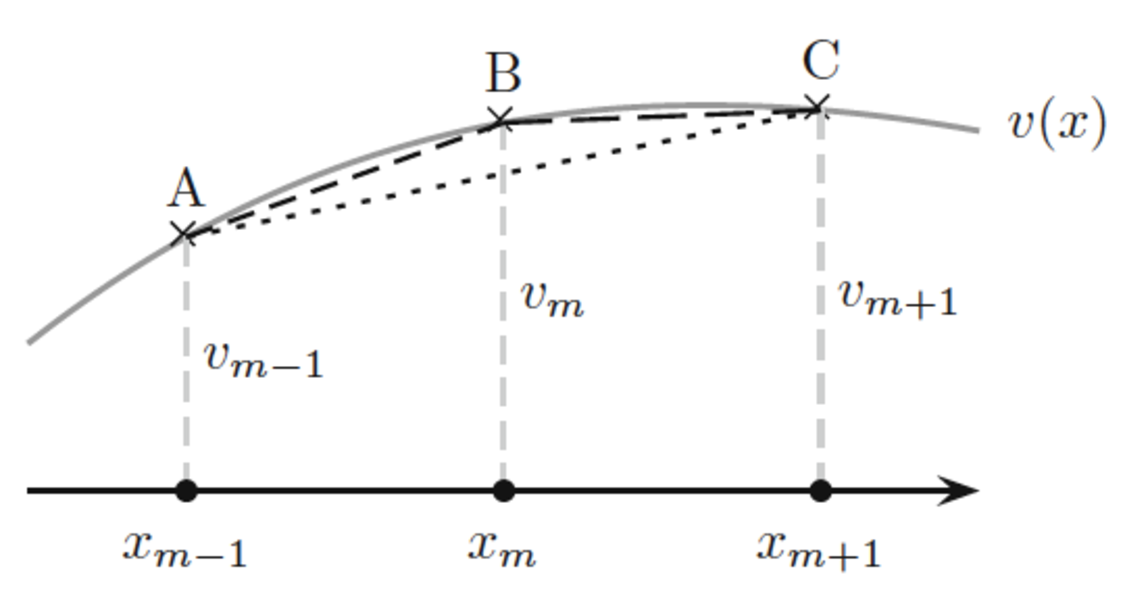
\includegraphics[width=0.5\linewidth]{figures/derivatives.pdf}
% \caption{The gradients of the chords $AB$ (backward), $BC$ (forward) and $AC$
% (central) are three possibilities of approximating the gradient of the tangent
% to the function $v(x)$(solid curve) at $B$.}\label{fig:back:derivatives_f}
% \end{figure}
%

Figure~\ref{fig:back:derivatives_f} represents a slice
of the function pictured in Figure~\ref{fig:back:generic_f} for a constant
value of $y$, the gradient of the function $v(\x)=v(x,y)$ at point $E$
($\x_{i,j}=(x_i,y_j)$) in the $x$-direction may be  approximated by the
gradients of any of the three chords $DE$, $EF$, or $DF$, each  case with its own degree of approximation. The slope of the backward chord at the point $E$
($\x_{i,j}=(x_i,y_j)$) can be associated to the the following one-directional
Taylor expansion in two-dimensions:
%
\begin{equation}\label{eq:back:1Dtaylor}
v(x-\Delta x,y)=v(x,y)-\frac{\partial v(x,y)}{\partial x}\Delta x + \frac{\partial^2 v(\xi,y)}{\partial x^2}\frac{\Delta x^2}{2},
\end{equation}
%
for some number $\xi\in\left((x,y),(x+\Delta x,y)\right)$, we choose the point
$\x_{i,j}=(x_i,y_j)$ and
%, adopting a notation \td{there is conflict with notation of partial derivatives and subindices}
%where $v_{i,j}$, $v_{x}(x_i,y_j)$ and $v_{xx}(x_i,y_j)$ are used to denote
%$v(x_i,y_j)$, $\frac{\partial v(x_i,y_j)}{\partial x}$, and
%$\frac{\partial^2 v(x_i,y_j)}{\partial x^2}$ respectively, we can
rearrange the previous expression to give:
$$
%v_{x}(x_i,y_j) =
\frac{\partial v(x_i,y_j)}{\partial x} = h_{x_i}^{-1}(v_{i,j}-v_{i-1,j}) + \frac{h_{x_i}}{2}\frac{\partial^2 v(\xi_i,y_j)}{\partial x^2}, \quad \xi_i\in(x_{i-1},x_{i}),
$$
where the subscript $i$ in $\xi_i$ reflects its dependence on $(x_i,y_j)$.
We have
$$
%v_x(x_i,y_j) =
\frac{\partial v(x_i,y_j)}{\partial x} = h_{x_i}^{-1}(v_{i,j}-v_{i-1,j})+R_{i,j} = h_{x_i}^{-1}(v_{i,j}-v_{i-1,j}) + \mathscr{O}(h_{x_i}).
$$

The remainder term, commonly referred to as the \emph{local truncation error}
$R_{i,j}$ (see~\cite{PapLieStr14} for a good discussion of error
distributions), corresponds to truncating the Taylor series
\eqref{eq:back:1Dtaylor}. When the local truncation error is neglected, we obtain the \emph{backward difference approxiamtion} of
$\frac{\partial v(x_i,y_j)}{\partial x}$ at the point $\x_{i,j}=(x_i,y_j)$.
The backward difference operator or \emph{upwind finite difference operator}
in the $x$-direction, $\Delta^{-}_{x}$, is defined by
%
\begin{equation}\label{eq:back:1DupwindOp}
\Delta^{-}_{x}v_{i,j}\equiv v_{i,j}-v_{i-1,j},
\end{equation}
%
and so $\frac{\partial v(x_i,y_j)}{\partial x} \approx h_{x_i}^{-1}
\Delta^{-}_{x}v_{i,j}$ with an error $\mathscr{O}(h_{x_i})$.

We chose the expansion \eqref{eq:back:1Dtaylor}, however we can proceed in a
similar fashion using the forward version of the Taylor series instead:
\begin{equation}\label{eq:back:1Dtaylor_b}
v(x+\Delta x,y)=
%v(x,y)+v_{x}(x,y)\Delta x + v_{xx}(\xi,y)\frac{\Delta x^2}{2},
v(x,y)+\frac{\partial v(x,y)}{\partial x}\Delta x + \frac{\partial^2 v(\xi,y)}{\partial x^2}\frac{\Delta x^2}{2}
\end{equation}
and by defining the \emph{forward finite difference operator} in the
$x$-direction, $\Delta^{+}_{x}$,
\begin{equation}\label{eq:back:1DforwardOp}
\Delta^{+}_{x}v_{i,j}\equiv v_{i+1,j}-v_{i,j},
\end{equation}
%
we obtain another approximation to the derivative of $v$ at the point
$\x_{ij}$,\linebreak $\frac{\partial v(x_i,y_j)}{\partial x} \approx h_{x_{i+1}}^{-1}
\Delta^{+}_{x}v_{i,j}$ now with an error of $\mathscr{O}(h_{x_{i+1}})$.

Finally, by defining the \emph{central finite difference operator} in the
$x$-direction, $\Delta^{0}_{x}$,
\begin{equation}\label{eq:back:1DcentralOp}
\Delta^{0}_{x}v_{i,j}\equiv v_{i+1,j}-v_{i-1,j},
\end{equation}
%
we find that $\frac{\partial v(x_i,y_j)}{\partial x}
\approx (h_{x_{i}} + h_{x_{i+1}})^{-1} \Delta^{0}_{x}v_{i,j}$
now with an error $\mathscr{O}\left((h_{x_{i}} + h_{x_{i+1}})^2\right)$. It is
possible to obtain more accurate approximations by including more terms
in the Taylor series \eqref{eq:back:1Dtaylor} and \eqref{eq:back:1Dtaylor_b}
before truncating it, obtaining higher order methods (see \cite{Dem97} for a
discussion in this direction).
% \td{\textbf{write}: still need to add derivation of the formulas for second derivatives}

In order to approximate second order derivatives (and most even-order derivatives), it is common to introduce another ``artificial" central approximation
\begin{equation}\label{eq:back:1DcentralOp}
\delta_{x}v_{i,j}\equiv v_{i+\frac12,j}-v_{i-\frac12,j},
\end{equation}
which makes use of intermediate points which are not on the grid. This approximation corresponds to the $\Delta$ approximation with a half-step $h_{x_i}/2$.
 Nevertheless, by computing $\delta_x(\delta_x)v_{i,j}$ we obtain
\begin{equation}\label{eq:back:1DcentralOp}
\delta_{x}(\delta_x v_{i,j})= v_{i+1,j}-2v_{i,j}+v_{i-1,j}.
\end{equation}
In the exact fashion as above, by considering both Taylor approximations \eqref{eq:back:1Dtaylor} and \eqref{eq:back:1Dtaylor_b}, adding them together adn evaluatng at the point $\x_{i,j}$ we obtain a centered finite difference approximation to the second derivative,
\begin{equation*}
\frac{\partial^2 v(x_i,y_j)}{\partial x^2} = h_{x_i}^{-2}(v_{i+1,j}-2v_{i,j}+v_{i-1,j})- \mathscr{O}(h_{x_i}^2)\approx h_{x_i}^{-2}\delta^2v_{i,j},
\end{equation*}
with a remainder term proportional to $h_{x_i}^2$.

This analysis can be repeated for approximating the partial derivative of the
function $v$ in the $y$-direction to obtain analogous results. Using the notation $v_{x}=\frac{\partial v}{\partial x}$, $v_{xx}=\frac{\partial^2 v}{\partial x^2}$, and where $h_{x_{\text{eff}}}=h_{x_i}+h_{x_{i+1}}$ we
summarize the results in Table~\ref{tab:back:findiff}

%\begin{table}[h!]\centering
\begin{equation}\label{tab:back:findiff}
\begin{array}{ll}
%\hline
%$1^{\text{st}}$ Order Forward operator in $x$-dir &
\Delta^{+}_{x} v_{i,j} = v_{i+1,j} - v_{i,j} = h_{x_{i+1}} v_{x} + \frac{1}{2}h_{x_{i}}^2 v_{xx} + \mathscr{O}(h_{x_{i+1}}^3) &
\text{\emph{Forward differences}} \\
% %\hline
% $1^{\text{st}}$ Order Forward operator in $y$-dir & $
\Delta^{+}_{y} v_{i,j} = v_{i,j+1} - v_{i,j} = h_{y_{i+1}} v_{y} + \frac{1}{2}h_{y_{i}}^2 v_{yy} + \mathscr{O}(h_{y_{i+1}}^3) &
\text{\emph{Forward differences}}\\
%\hline
%$1^{\text{st}}$ Order Upwind operator in $x$-dir &
\Delta^{-}_{x} v_{i,j} = v_{i,j} - v_{i-1,j} = h_{x_{i}} v_{x} - \frac{1}{2}h_{x_{i}}^2 v_{xx} + \mathscr{O}(h_{x_{i}}^3) &
\text{\emph{Upwind differences}} \\
% %\hline
% $1^{\text{st}}$ Order Upwind operator in $y$-dir & $
\Delta^{-}_{y} v_{i,j} = v_{i,j} - v_{i,j-1} = h_{y_{i}} v_{y} - \frac{1}{2}h_{y_{i}}^2 v_{yy} + \mathscr{O}(h_{y_{i}}^3) &
\text{\emph{Upwind differences}}\\
% %\hline
% %$1^{\text{st}}$ Order Central operator in $x$-dir &
\Delta^{0}_{x} v_{i,j} = v_{i+1,j} - v_{i-1,j} = h_{x_{\text{eff}}} v_{x} +
\frac{1}{6}h_{x_{\text{eff}}}^3 v_{xxx} + \mathscr{O}(h_{x_{\text{eff}}}^5) &
\text{\emph{Central differences}} \\
% %\hline
% $1^{\text{st}}$ Order Central operator in $y$-dir  & $
\Delta^{0}_{y} v_{i,j} = v_{i,j+1} - v_{i,j-1} = h_{y_{\text{eff}}} v_{y} + \frac{1}{6}h_{y_{\text{eff}}}^3 v_{yyy} + \mathscr{O}(h_{y_{\text{eff}}}^5) &
\text{\emph{Central differences}} \\
% %\hline
% %$2^{\text{nd}}$ Order Central operator in $x$-dir &
\delta^{2}_{x} v_{i,j} = v_{i+1,j} - 2v_{i,j}+v_{i-1,j} = h_{x_{\text{eff}}}^2 v_{xx} + \frac{1}{12}h_{x_{\text{eff}}}^4 v_{xxxx} + \mathscr{O}(h_{x_{\text{eff}}}^6) &
\text{\emph{Central differences}} \\
% %\hline
% $2^{\text{nd}}$ Order Central operator in $y$-dir & $
\delta^{2}_{y} v_{i,j} = v_{i,j+1} - 2v_{i,j} + v_{i,j-1} = h_{y_{\text{eff}}}^2 v_{yy} + \frac{1}{12}h_{x_{\text{eff}}}^4 v_{yyyy} + \mathscr{O}(h_{y_{\text{eff}}}^6) &
\text{\emph{Central differences}}
% %\hline
\end{array}
\end{equation}
%\caption{Finite difference operators and Taylor Expansions $(h_{y_{\text{eff}}}=h_{y_{i}}+h_{y_{i+1}})$.}
%\end{table}

\subsection{Shishkin Mesh in 1D}
\label{back:convdiff:shihs1D}

In order to obtain an accurate numerical solution of BVPs with singularly
perturbed convection-diffusion problems described by equation
\eqref{eq:back:1Dbvp}, we require special discretization techniques.
As mentioned in Section~\ref{back:convdiff}, we focus on the approach of
using upwind or central finite difference schemes posed on a Shishkin mesh, an
approach described described, e.g., in~\cite[\S~5]{Sty05}
or~\cite{FarHegMilOriShi00,KopOri10,LinSty01,MilOriShi96}. In this subsection
we introduce the one-dimensional Shishkin mesh and describe its construction.
For a comprehensive treatment of layer-adapted meshes for convection-diffusion
problems see the monograph \cite{Lin10}. Without loss of generality, we assume
that $\omega_x\gg \epsilon >0$ and $\beta\geq 0$ and that the parameters of
the problem \eqref{eq:back:1Dbvp}, i.e., $\epsilon,\omega_x,\beta,f,g_0,$ and
$g_1$, are chosen so that the solution $u(x)$ has one boundary layer close to
the point $x=1$.
% \td{\textbf{fix}: the underbrace for $h_{x}$ in the Figure~\ref{fig:back:shmesh1D} looks weird.}
%
\begin{figure}[h!]
\centering
\begin{tikzpicture}
%%%%% x-axis:
\draw[thick,-] (0,1) -- (11, 1);
\draw[thick,line width=1mm] (0,0.7)   -- (0, 1.3);
\draw[thick,line width=1mm] (11,0.7)  -- (11, 1.3);
\draw[thick,line width=1mm] (8.3,0.7) -- (8.3, 1.3);
\foreach \i in {.83,1.66,2.49,3.32,4.15,4.98,5.81,6.64,7.47}{
  \draw[thick,-] (\i,0.8) -- (\i, 1.2);
}
\foreach \ii in {8.57,8.84,9.11,9.34,9.61,9.88,10.15,10.42,10.69}{
  \draw[thick,-] (\ii,0.8) -- (\ii, 1.2);
}
\node[below] at (0,0.7)  {$x_{0}$};
\node[above] at (0,1.3)  {$0$};
\node[below] at (11,0.7) {$x_{N}$};
\node[above] at (11,1.3) {$1$};
\node[below] at (8.3,0.7) {$x_{n}$};
\node[above] at (8.3,1.3) {$1-\tau_x$};
\draw [decorate,decoration={brace,amplitude=5pt},xshift=0pt,yshift=-5pt] (4.2,1) -- (3.3,1) node [black,midway,yshift=0pt] {};
\node[below] at (3.8,0.7) {$H_{x}$};
\draw [decorate,decoration={brace,amplitude=5pt},xshift=0pt,yshift=-5pt] (9.6,1) -- (9.4,1) node [black,midway,yshift=0pt] {};
\node[below] at (9.5,0.7) {$h_{x}$};
\end{tikzpicture}
\caption{Illustration of a one-dimensional Shishkin mesh.}
\label{fig:back:shmesh1D}
\end{figure}
%
%\begin{figure}[h!]
%\centering
%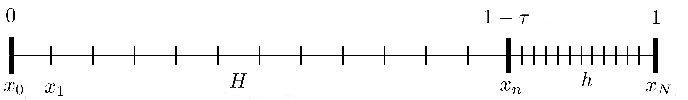
\includegraphics[width=0.85\linewidth]{figures/shmesh.pdf}
% %\\[2ex]
% %\includegraphics[width=0.5\linewidth]{figures/analytic_solution}
% \caption{Illustration of a one-dimensional Shishkin mesh.}
% \label{fig:back:shmesh1D}
% \caption{Illustration of a Shishkin mesh (top) and plot of the analytic
% solution of the problem \eqref{eq:back:1Dbvp} with $\epsilon=0.01$, $\omega=1$,
% $\beta=0$, $f(x)\equiv 1$, and $g_0=g_1=0$ (bottom). For $N=48$ the
% mesh transition point is $1-\tau_x=0.9226$.}\label{fig:back:shmesh1D}
%\end{figure}

In short, Shishkin meshes are formed by an overlapping union of piecewise
uniform meshes, with their respective sizes and mesh transition (or interface)
points adapted to the expected width of the boundary layers in the solution.
Suppose that an even integer $N\geq 4$ defining the number of intervals
constituting the Shishkin mesh is given, and suppose that the
\emph{mesh transition parameter}, $\tau_x$, fulfills
%
\begin{equation}\label{eq:back:tau_x}
\tau_x \equiv 2\frac{\epsilon}{\omega} \ln N \leq \frac{1}{2}.
\end{equation}
%
The inequality in \eqref{eq:back:tau_x} means that
%
\begin{equation}\label{eq:back:epsi}
\epsilon \leq \frac{\omega}{4 \ln N},
\end{equation}
%
which is a natural assumption since $\omega\gg \epsilon$, and the number of
mesh points usually is not exponentially large relative to $\epsilon$.
The \emph{mesh transition point} $1-\tau_x$ then will be close to $x=1$, and
the boundary layer will be contained in the (small) interval $[1-\tau_x, 1]$.
The idea of the Shishkin mesh discretization of the interval $[0,1]$ is to use
the same number of equidistantly distributed mesh points in each of the
subintervals $[0,1-\tau_x]$ and $[1-\tau_x,1]$ as can bee seen in
Figure~\ref{fig:back:shmesh1D}. Thus, if we denote
%
\begin{equation}\label{eq:back:nHh1D}
n\equiv \frac{N}{2},\quad H_x\equiv\frac{1-\tau_x}{n},\quad\text{and}\quad h_x\equiv \frac{\tau_x}{n},
\end{equation}
%
then the $N+1$ mesh points of the Shishkin mesh are given by
%
$$x_{i}\equiv iH_x, \quad i=0,\dots,n, \qquad x_{i}\equiv 1-(N-i)h_x, \quad i=n+1,\dots,N.$$
%
Here $x_0=0$ and $x_N=1$, so that the mesh consists of $N-1$ interior mesh
points, where the mesh point $x_n$ is exactly at the transition point
$1-\tau_x$. The ratio between the mesh sizes in the two subdomains is

\begin{align*}
\frac{h_{x}}{H_{x}} = \frac{\tau_x}{1-\tau_x} = \tau_x + \mathscr{O}(\tau_x^2),
\end{align*}
which is usually much less than $1$.

Any Shishkin mesh discretization naturally leads to a decomposition of the
given domain into overlapping subdomains. In our one-dimensional model problem
the domain is the interval $[0,1]$, and the overlapping subdomains are the
intervals $[0,1-\tau_x+h_x]$ and $[1-\tau_x-H_x,1]$.
The width of the overlap is $H_x+h_x=2/N$, and the mesh transition point
$x_n=1-\tau_x$ is the only mesh point in the overlap.
An illustration of a Shishkin mesh is shown in Figure~\ref{fig:back:shmesh1D},
and a plot of the (explicitly known) analytic solution of the problem
\eqref{eq:back:1Dbvp} with $\epsilon=0.03$, $\omega=1$, $\beta=0$,
$f(x)\equiv 1$, and $g_0=g_1=0$ is shown in Figure~\ref{fig:back:1D_analytic_sol}
 % \td{\textbf{fix}: Figure~\ref{fig:back:1D_analytic_sol} looks weird, chosen parameters make the transition point ``too far away"};
cf.~\cite[Example~3.1]{Sty05}. Choosing, for example, $N=48$ gives the mesh
transition point $1-\tau_x=0.7677$ (these parameters were chosen for
presentation purposes only, if we choose $\epsilon=0.01$ while keeping the
other parameters constant we obtain $1-\tau_x=0.9226$).

\begin{figure}[h!]
\centering
\begin{tikzpicture}[scale=0.43,declare function={ep=0.03;}]
%%%%% x-axis:
\draw[thick,-] (0,1) -- (11, 1);
\draw[thick,line width=1mm] (0,0.7)   -- (0, 1.3);
\draw[thick,line width=1mm] (11,0.7)  -- (11, 1.3);
\draw[thick,line width=1mm] (8.3,0.7) -- (8.3, 1.3);
\draw[dashed, color=gray] (8.3,0.7) -- (8.3, 10.7);
\foreach \i in {.83, 1.66, 2.49, 3.32, 4.15, 4.98, 5.81, 6.64, 7.47, 8.57, 8.84, 9.11, 9.34, 9.61, 9.88, 10.15, 10.42, 10.69}{
  \draw[thick,-] (\i,0.8) -- (\i, 1.2);
}
% \foreach \ii in {8.57,8.84,9.11,9.34,9.61,9.88,10.15,10.42,10.69}{
%   \draw[thick,-] (\ii,0.8) -- (\ii, 1.2);
% }
\node[below] at (0,0.7)  {$0$};
\node[below] at (8.3,0.7) {$1-\tau_x$};
\node[below] at (11,0.7) {$1$};
\draw[scale=11,domain=0:1,smooth,variable=\x, color=darkgray] plot ({\x},{.1+(\x - (exp(-(1-\x)/ep) - exp(-1/ep))/(1-exp(-1/ep)))});
\end{tikzpicture}
\caption{Analytic solution of problem \eqref{eq:back:1Dbvp} with $\epsilon=0.03$, $\omega=1$, $\beta=0$, $f(x)\equiv 1$, and $g_0=g_1=0$. For $N=48$ the mesh transition point is $1-\tau_x = 0.7677$.}
\label{fig:back:1D_analytic_sol}
\end{figure}
%
% \begin{figure}[h!]
% \centering
% \missingfigure[figwidth=6cm]{Solution to \eqref{eq:back:1Dbvp}.}
% \caption{Plot of the analytic solution of the problem \eqref{eq:back:1Dbvp} with $\epsilon=0.01$, $\omega=1$, $\beta=0$, $f(x)\equiv 1$, and $g_0=g_1=0$. For $N=48$ the mesh transition point is $1-\tau_x = 0.9226$.}
% \label{fig:back:1D_analytic_sol}
% \end{figure}

\subsection{Shishkin Mesh in 2D}
\label{back:convdiff:shihs2D}

In the case of two spacial dimensions, we can create various types of Shishkin
meshes depending on the number of outflow boundary layers in each coordinate
direction for a given problem. In the case of one boundary layer in one
direction and no layer in the other direction we will use a combination of a
regular discretization in the coordinate direction without a boundary layer
with a Shishkin mesh discretization in the coordinate direction with an
outflow boundary layer. In the other case we will use two Shishkin meshes, one
for each coordinate direction.
% \td{\textbf{write}: still need to mention in the previous subsections the ``well posedness" of the problem and its relation to the number of boundary layers}

\subsubsection{2.1.4.1. \ One Outflow Boundary Layer}
The simplest generalization of the Shishkin mesh for the case of two spacial
dimensions is to use a discretization approach that combines a regular mesh in
one coordinate direction (say $x$) with a Shishkin mesh discretization
in the other coordinate direction (say $y$).
%
\begin{figure}[h!]
\begin{minipage}[b]{0.4\textwidth}
\centering
\begin{tikzpicture}[scale = 0.4]
%%%% Rectangle:
\draw (0,0) rectangle (10, 10);
%%%% horizontal lines and $y$
\node[left] at (0,10) {$1$};
\draw (0,8) node[left] {$1-\tau_y$} -- (10,8);
\node[left] at (0,0) {$0$};
\node[below] at (0,0) {$0$};
\node[below] at (10,0) {$1$};
%%%% Black dots:
\draw[black,fill=black] (0,8) circle (0.5ex);
%%%% Tile labels
\node at (5,4) {$\Omega_1$};
\node at (5,9) {$\Omega_2$};
\end{tikzpicture}
\end{minipage}
  \hspace*{3em}
\begin{minipage}[b]{0.4\textwidth}
\centering
\begin{tikzpicture}[scale = 0.4]
%%%% Rectangle:
\draw (0,0) rectangle (10, 10);
%%%% horizontal lines and $y$
\node[left] at (0,10) {$y_M$};
\draw (0,9.5) -- (10,9.5);
\draw (0,9)  -- (10,9);
\draw (0,8) node[left] {$y_m$}  -- (10,8);
\draw (0,8.5)  -- (10,8.5);
\draw (0,6)  -- (10,6);
\draw (0,4)  -- (10,4);
\draw (0,2)  -- (10,2);
\node[left] at (0,0) {$y_0$};
%%%% vertical lines and $x$:
\node[below] at (0,0) {$x_0$};
\draw (2,0)  -- (2,10);
\draw (4,0)  -- (4,10);
\draw (6,0)  -- (6,10);
\draw (8,0)  -- (8,10);
\node[below] at (10,0) {$x_N$};
%%%% Black dots:
\draw[black,fill=black] (0,8) circle (0.5ex);
%%%% Tile labels
\draw (5,0) node[below] {$H_x$};
\draw (10,3) node[right] {$H_y$};
\draw (10,8.7) node[right] {$h_y$};
\end{tikzpicture}
\end{minipage}
%\includegraphics[width=0.9\linewidth]{figures/simpleShish2D3.pdf}
\caption{Division of the domain and Shishkin mesh for equation \eqref{eq:back:nDbvp} with one outflow exponential layer.}
\label{fig:back:shmesh2Da}
\end{figure}

Given now two even positive integers $N\geq 4$ and $M\geq 4$ that denote the
number of mesh intervals used in each coordinate direction, we let the
transition parameter $\tau_y$ that will be used to specify where the mesh
changes from coarse to fine in the $y$-direction, be defined by
%
\begin{equation}\label{eq:back:tau_y}
\tau_y~\equiv~\min\left\{\frac{1}{2},2\frac{\epsilon}{\omega_y}  \ln M\right\}.
\end{equation}
%
Since we assume $\omega_y\gg \epsilon$ (or equivalently that
$\epsilon \leq CM^{-1}$), we will have
$\tau_y~=~2\frac{\epsilon}{\omega_y}\ln M~\ll~1$,
so that in this case the \emph{mesh transition point} $1-\tau_y$ will be very
close to the boundary $y=1$. By assuming that the parameters of the problem,
i.e. $\epsilon, \om, \beta$, $f$, and  $g$, are chosen so that the solution
$u(x,y)$ has one boundary layer at $y=1$. In particular, this is achieved by
assuming that $\om=[0,\omega_y]^T$, and $\omega_y>0$. The use of this Shishkin
mesh discretization scheme will divide the domain $\Omega$ into two overlapping
subdomains, $\overline{\Omega}=\Omega_{1}\cup\Omega_{2}$, where
%
$$
\Omega_{1}=[0,1]\times[0,1-\tau_y],\quad\Omega_{2}=[0,1]\times[1-\tau_y,1].
$$
%
This subdivision is shown in the left side of Figure~\ref{fig:back:shmesh2Da}.
% Each subdomain is then decomposed into $N/2\times N/2$ rectangles with $N/2$ interior nodes in each subdomain.
%

Let $m\equiv \frac{M}{2}$, if we denote by $H_x$ the mesh width in the $x$-
direction and by $h_y$ and $H_y$ the mesh widths inside and outside the
boundary layer in the $y$-direction, i.e.,
%
\begin{equation}\label{eq:back:Hh2D}
H_x\equiv\frac{ 1}{N},
\;\;\quad
h_y\equiv\frac{\tau_y}{m},
\;\;\quad\mbox{and}\;\;\quad
H_y\equiv\frac{( 1-\tau_y)}{m},
 \end{equation}
%\begin{equation}\label{eq:back:tau}
%h_i=
%\begin{cases}h_1\equiv\frac{2( 1-\tau_x)}{N} &\mbox{for}\;\; i=0,\ldots,n \\
%h_2\equiv\frac{\tau_x}{N} &\mbox{for}\;\; i=n+1,\ldots,N. \end{cases}
%\quad
%%\text{and}\quad
%k_i=
%\begin{cases}k_1\equiv\frac{2( 1-\tau_y)}{N} &\mbox{for}\;\; i=0,\ldots,n \\
%h_2\equiv\frac{\tau_y}{N} &\mbox{for}\;\; i=n+1,\ldots,N. \end{cases}
%\end{equation}
%,\quad H\equiv\frac{1-\tau}{n},\quad h\equiv \frac{\tau}{n},
%
then the $(N+1)\times(M+1)$ nodes of the Shishkin mesh are given by
\[
\Omega_D=\{(x_i,y_j)\in\overline{\Omega}:i=0,\ldots,N, j=0,\ldots,M\},
\]
where
%
\begin{equation}\label{eq:back:shishmeshnodes}
x_i\equiv iH_x,\;\mbox{for}\;\; i=0,\ldots,N,
\quad \mbox{ and } \quad
y_j\equiv
\begin{cases} jH_y &\mbox{for}\;\; j=0,\ldots,m, \\
1-(N-j)h_y &\mbox{for}\;\; j=m+1,\ldots,M. \end{cases}
\end{equation}
%
%$$x_{i}\equiv iH, \quad i=0,\dots,n, \qquad x_{i}\equiv 1-(N-i)h, \quad i=n+1,\dots,N.$$
%
The mesh is constructed by drawing lines parallel to the coordinate axes
through these mesh points; see the right side of
Figure~\ref{fig:back:shmesh2Da}. Here $x_0=0$, $y_0=0$ and $x_N=1$, $y_M=1$
so that the mesh consists of $N-1$ interior nodes in each direction and where
the node $y_m$ is exactly at the transition point $1-\tau_y$ in the $y$-
direction. In contrast to the one-dimensional case where the overlapping
subdomains intersect in exactly one grid point, in this two-dimensional case
we have a whole row of grid points in common. The $N-1$  nodes with vertical
coordinate equal to $y_n=1-\tau_y$ are the grid points in the overlap. It is
clear that the mesh widths on $\Omega_{1}$ satisfy
$1/N\leq H_x,\, H_y\leq 2/M$, so the mesh is coarse in this domain. On the
other hand, $h_y$ is $\mathscr{O}(\epsilon M^{-1}\log(M))$, so on $\Omega_2$
the mesh is coarse in the $x$ direction and fine in the $y$ direction. The
ratio between the different mesh sizes in the $y$ direction is
%
\[\frac{h_y}{H_y}=\frac{\tau_y}{1-\tau_y}=\tau_y+\mathscr{O}(\tau_y^2) \ll 1.\]
%


\begin{example}
We consider the BVP \eqref{eq:back:nDbvp} defined on $\Omega=(0,1)\times(0,1)\in\mathbb{R}^{2}$ with $\beta=0$, $f=0$ and boundary conditions determined by the function
%
\begin{equation}\label{analytic_solution}
u(x,y)=(2x-1)\left(\frac{1-e^{(2y-2)/\epsilon}}{1-e^{-2/\epsilon}}\right).
\end{equation}
%
A three-dimensional rendering of the analytic solution to this problem is
shown in Figure~\ref{fig:back:2D_analytic_sol} for the case $\epsilon=0.01$.
In most parts of the domain $\Omega$, the values of the solution $u(x,y)$
closely resemble the ones given by the \emph{inflow boundary} condition
$u(x,0)=2x-1$, except in a vicinity of the \emph{outflow boundary} where they
abruptly change to the constant values $u(x,1)~=~0$. The boundary conditions at
$x=0$ and $x=1$ satisfy $u(0,y)\approx-1$ and $u(1,y)\approx 1$ respectively
(see \cite[Example 6.1.1]{ElmSilWat14} where a similar problem is presented)
and its values also change drastically as they approach the outflow
boundary, where they change from $\approx-1$ or $\approx 1$ to $0$.
The portion of the domain where these changes occur is proportional to
$\epsilon$ and it is determined by the function $e^{(2-2y)/\epsilon}$, thus,
when small enough values of $\epsilon$ are chosen, the changes in the function
$u$ occur abruptly enough and in a portion of the domain that is small enough
so that the solution of \eqref{eq:back:nDbvp} presents an exponential boundary
layer in this particular region of the domain.
%
\begin{figure}[h!]
\begin{minipage}[t]{0.5\linewidth}
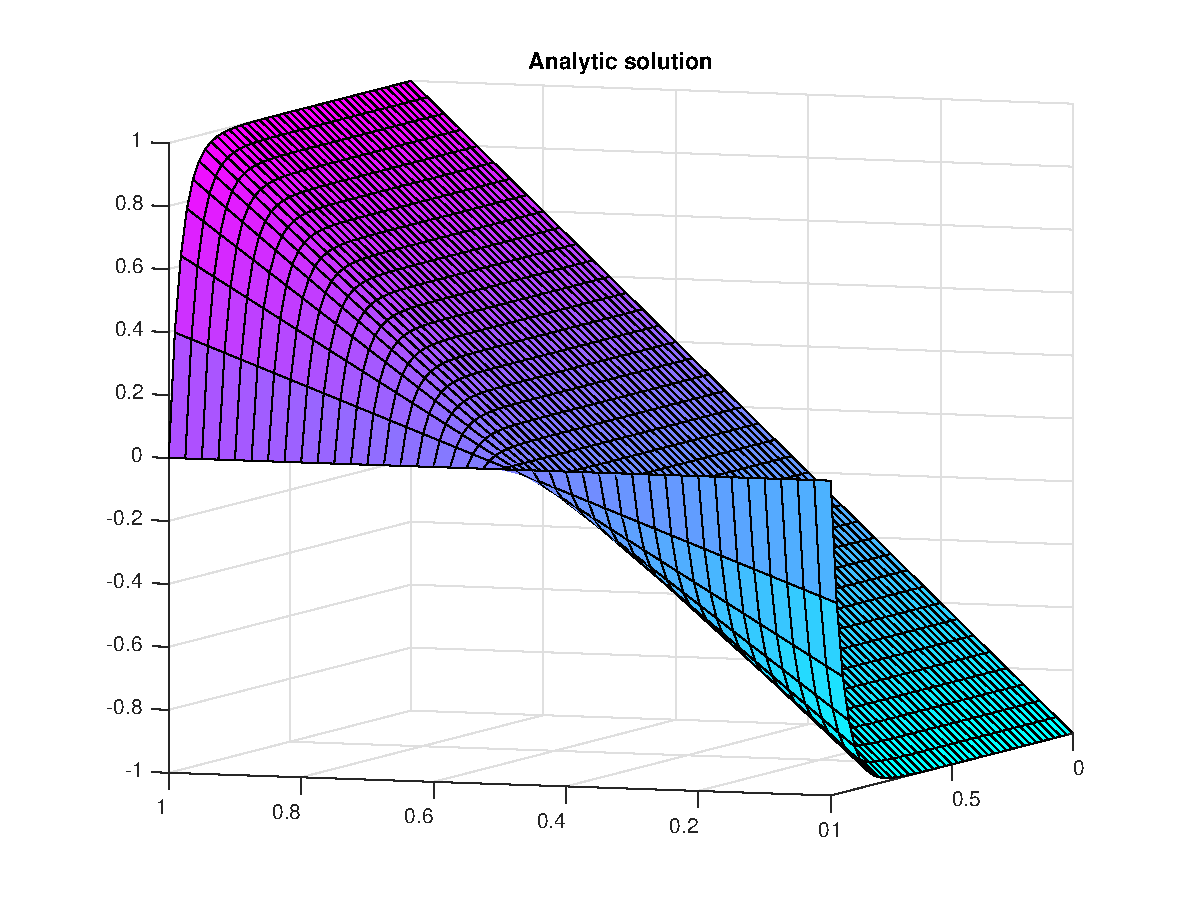
\includegraphics[width=0.83\linewidth]{figures/analytic_sol_new}
\end{minipage}
%
\begin{minipage}[t]{0.5\linewidth}
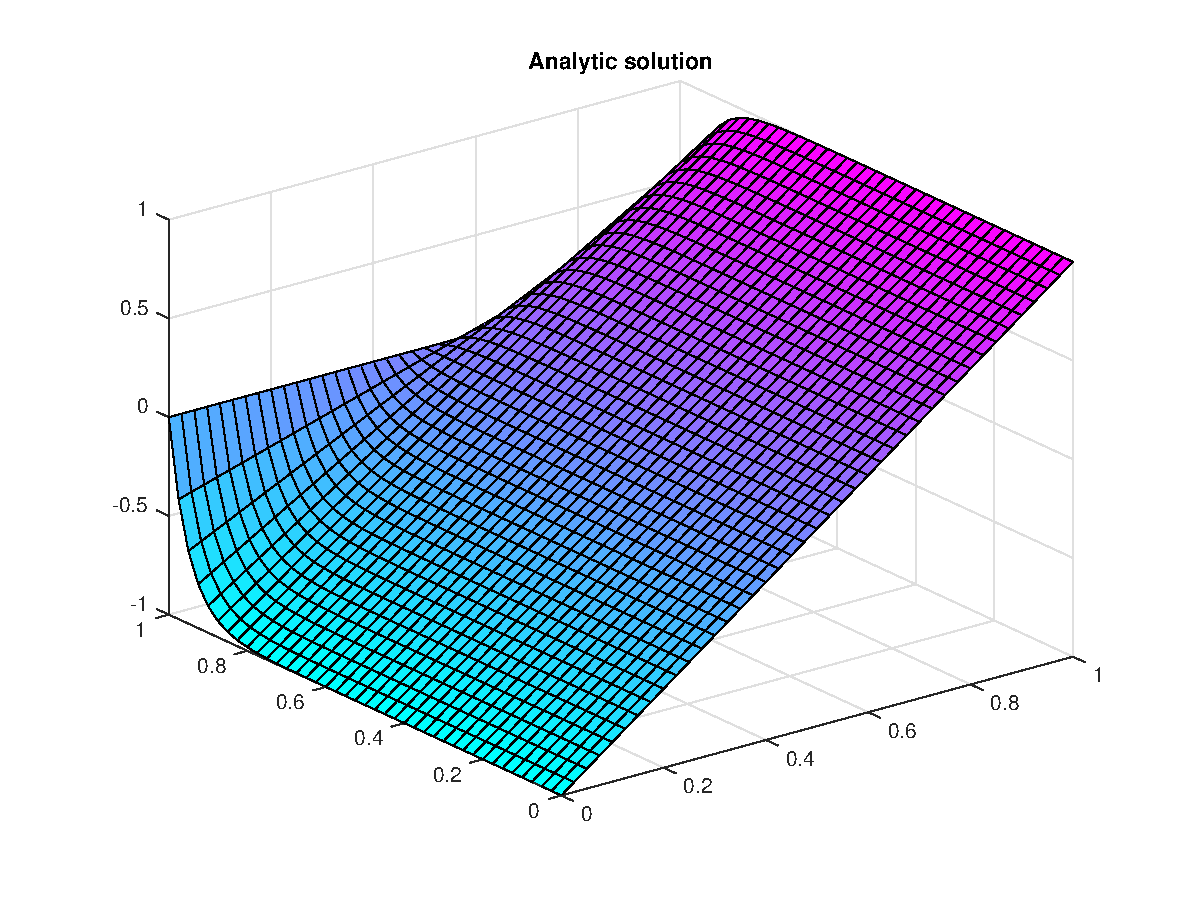
\includegraphics[width=0.83\linewidth]{figures/analytic_sol_new2b}
\end{minipage}
\caption{Three-dimensional surface plot of the analytic solution of
\eqref{eq:back:nDbvp} with $n=2$, $\omega_x,\beta=0$ and $\epsilon=10^{-1}$ for two different viewing angles.}
\label{fig:back:2D_analytic_sol}
\end{figure}

This will be the main example used in future chapters to exemplify the theoretical results obtained for two-dimensional problems.
\end{example}

\subsubsection{2.1.4.2. \ Two Outflow Boundary Layers}
In the case of two outflow boundaries, we can now use a one dimensional Shishkin mesh in each coordinate direction.
Again, given two even positive integers $N\geq 4$ and $M\geq 4$ that denote the
number of mesh intervals used in each coordinate direction, let the transition
parameters $\tau_x$ and $\tau_y$, that will be used to specify where the mesh
changes from coarse to fine, be defined by
%
\begin{equation}\label{eq:back:tau_xy}
\tau_x \equiv \min\left\{\frac12,2\frac{\epsilon}{\omega_x}  \ln N\right\}\quad\text{ and }\quad\tau_y \equiv \min\left\{\frac12,2\frac{\epsilon}{\omega_y} \ln M\right\}.
\end{equation}
%
Once again, since we assume $\omega_x,\omega_y\gg \epsilon$, we will usually
have $\tau_x=2\frac{\epsilon}{\omega_x}  \ln N\ll 1$ and
$\tau_y=2\frac{\epsilon}{\omega_y} \ln M\ll 1$, so that in both spacial
directions the \emph{mesh transition points} $1-\tau_x$ and $1-\tau_y$ will be
located very close to the boundary with $x=1$ in the $x$-direction and very
close to the boundary with $y=1$ in the $y$-direction.
%Otherwise, the analysis can be carried out using standard techniques.

In the case of this discretization scheme the domain $\Omega$ is divided into
four overlapping subdomains, where
$\overline{\Omega}=\Omega_{1}\cup\Omega_{2}\cup\Omega_{3}\cup\Omega_{4}$.
That is, by again letting $n\equiv \frac{N}{2}$ and $m\equiv \frac{M}{2}$, the
mesh division divides $\Omega$ into a set of 4 subdomains, each of
them consisting of $n\times m$ rectangles giving $nm$ interior nodes in each
subdomain. This subdivision is shown on the left side of
Figure~\ref{fig:back:shmesh2Db}.
%
\begin{figure}[h!]
% \includegraphics[width=0.8\linewidth]{figures/Shish2D}
\hspace*{-2em}
\begin{minipage}[b]{0.5\textwidth}
\centering
\begin{tikzpicture}[scale = 0.4]
%%%% Rectangle:
\draw (0,0) rectangle (10, 10);
%%%% horizontal lines and $y$
\node[left] at (0,10) {$1$};
\draw (0,8) node[left] {$1-\tau_y$} -- (10,8);
\node[left] at (0,0) {$0$};
\node[below] at (0,0) {$0$};
\node[below] at (10,0) {$1$};
\draw (8,0) node[below] {$1-\tau_x$} -- (8,10);

%%%% Black dots:
\draw[black,fill=black] (0,8) circle (0.5ex);
\draw[black,fill=black] (8,8) circle (0.5ex);
\draw[black,fill=black] (8,0) circle (0.5ex);
%%%% Tile labels
\node at (4,4) {$\Omega_x$};
\node at (9,4) {$\Omega_2$};
\node at (4,9) {$\Omega_3$};
\node at (9,9) {$\Omega_4$};
\end{tikzpicture}
\end{minipage}
%
\hspace*{1em}
%
\begin{minipage}[b]{0.5\textwidth}
\centering
\begin{tikzpicture}[scale = 0.4]

%%%% Rectangle:
\draw (0,0) rectangle (10, 10);

%%%% horizontal lines and $y$
\foreach \point in {2,4,6,8,8.5,9,9.5}
\draw (0,\point) -- (10,\point);
\node[left] at (0,10) {$y_M$};
\node[left] at (0,8) {$y_m$};
\node[left] at (0,0) {$y_0$};

%%%% vertical lines and $x$:
\foreach \point in {2,4,6,8,8.5,9,9.5}
\draw (\point,0) -- (\point,10);
\node[below] at (0,0) {$x_0$};
\node[below] at (8,0) {$x_n$};
\node[below] at (10,0) {$x_N$};

%%%% Black dots:
\draw[black,fill=black] (0,8) circle (0.5ex);
\draw[black,fill=black] (8,8) circle (0.5ex);
\draw[black,fill=black] (8,0) circle (0.5ex);

%%%% Tile labels
\draw (5,10) node[above] {$H_x$};
\draw (8.8,10) node[above] {$h_x$};
\draw (10,2.7) node[right] {$H_y$};
\draw (10,8.7) node[right] {$h_y$};
\end{tikzpicture}
\end{minipage}
%\includegraphics[width=0.9\linewidth]{figures/simpleShish2D3.pdf}
\caption{Division of the domain and Shishkin mesh for equation
\eqref{eq:back:nDbvp} with two outflow exponential layers.}
\label{fig:back:shmesh2Db}
\end{figure}

If we denote the mesh widths outside and inside the respective boundary layers
by $H_x$, $h_x$ and $H_y$, $h_y$, i.e.,
%
\begin{eqnarray*}
H_{x}\equiv\frac{( 1-\tau_x)}{n}, \qquad
h_{x}\equiv\frac{\tau_x}{n},\qquad
H_{y}\equiv\frac{( 1-\tau_y)}{m},\qquad
h_{y}\equiv\frac{\tau_y}{m},
\end{eqnarray*}
then the four overlapping subdomains are given by
%
\begin{eqnarray}\label{eq:back:subdomains_a}
\Omega_{1}=&[0,1-\tau_x+h_x)\times[0,1-\tau_y+h_y),\qquad\Omega_{2}&=(1-\tau_x-H_x,1]\times[0,1-\tau_y+h_x),\nonumber\\
\Omega_{3}=&[0,1-\tau_x+h_x)\times(1-\tau_y-H_y,1],\qquad\Omega_{4}&=(1-\tau_x-H_x,1]\times(1-\tau_y-H_y,1],\nonumber\\
\end{eqnarray}
%
the $(N+1)\times(M+1)$ nodes of the two-dimensional Shishkin mesh are now given
by
$$
\Omega_D=\{(x_i,y_j)\in\overline{\Omega}:i=0,\ldots,N, j=0,\ldots,M\},
$$
where
%
$$
%\hspace*{-4em}
x_i\equiv
\begin{cases} iH_x &\mbox{for}\;\; i=0,\ldots,n \\
1-(N-i)h_x &\mbox{for}\;\; i=n+1,\ldots,N, \end{cases},
$$
%\quad
and
$$
y_j\equiv
\begin{cases} jH_y &\mbox{for}\;\; j=0,\ldots,m \\
1-(M-j)h_y &\mbox{for}\;\; j=m+1,\ldots,M. \end{cases}
$$
%
The mesh is constructed by drawing lines parallel to the coordinate axes
through these mesh points, i.e., the mesh is obtained by a tensor product of
two one-dimensional piecewise uniform meshes; see the right side of
Figure~\ref{fig:back:shmesh2Db}. Here $x_0=0$, $y_0=0$ and $x_N=1$, $y_M=1$
so that the mesh consists of $N-1$ and $M-1$ interior nodes in each respective
direction, where the node $x_n$ is exactly at the transition point $1-\tau_x$
and the node $y_n$ is exactly at the transition point $1-\tau_y$.
It is clear that the mesh widths on $\Omega_{1}$ satisfy
$1/N\leq H_x\leq 2/N$ and $1/M\leq H_y\leq 2/M$, so the mesh is coarse in this
domain. On the other hand, $h_x$ and $h_y$ are
$\mathscr{O}(\epsilon N^{-1}\log(N))$ and
$\mathscr{O}(\epsilon M^{-1}\log(M))$ respectively,
so the mesh is very fine on $\Omega_{4}$. On $\Omega_{2}$ and $\Omega_{3}$, the
mesh is coarse in one direction and fine in the other direction. The ratio
between the different mesh sizes in the $x$-coordinate direction is again
%
\[\frac{h_x}{H_x}=\frac{\tau_x}{1-\tau_x}=\tau_x+\mathscr{O}(\tau_x^2) \ll 1.\]
%
and similarly for the ratio $\frac{h_y}{H_y}$.
% \td{\textbf{add}: need to add a picture of a solution for a 2D boundary-layer problem with 2 layers (double glazing problem maybe?)}

\subsection{Approximation of BVPs}
\label{back:convdiff:BVPapprox}
In the most general setting, in order to find a finite difference
representation of a BVP, both the PDE and the boundary conditions need to be
replaced with a suitable approximation. Here, the approximation process will be
illustrated through the Dirichlet problem of the convection diffusion
equation posed on the square domain $\Omega=(0,1)\times(0,1)$.

We first denote the internal grid points where the equation will be
approximated~by
\[
\Omega_D=\{(x_i,y_j);i=1,\ldots,N-1;\;j=1,\ldots,M-1\},
\]
and denote the grid points on the boundary by $\partial\Omega_D$ and the
entire grid by $\overline{\Omega}_D=\Omega_D\cup\partial\Omega_D$.
Since boundary conditions of Dirichlet-type are exact in the
boundary nodes, an approximation of the boundary conditions is not needed and
we can focus our attention on the approximation of the PDE. We proceed to
evaluate the PDE of our two-dimensional BVP~\eqref{eq:back:nDbvp} at the
internal grid points of the mesh to obtain
%
\begin{equation}\label{eq:back:2Dpde}
-\epsilon \Delta u(x_i,y_j) + \omega(x_i,y_j)\cdot \nabla u(x_i,y_j) + \beta(x_i,y_j) u(x_i,y_j) = f(x_i,y_j).
\end{equation}
%
Using the standard finite difference operators
(see Table~\ref{tab:back:findiff} or e.g., \cite[\S~4]{Sty05})
to represent the first and second derivative terms and using the notation
$\omega_{ij}=\omega(x_i,y_j)$, $\beta_{ij}=\beta(x_i,y_j)$, $f_{ij}=f(x_i,y_j)$, etc., leads to the the upwind scheme approximation
%
\begin{equation}\label{eq:back:2DpdeO}
-\epsilon \left( h_{x_{i}}^{-2}\delta^2_x u_{ij} + h_{y_{j}}^{-2}\delta^2_y u_{ij}\right) + \omega^x_{ij} h_{x_{i}}^{-1}\Delta^{-}_{x}u_{ij} + \omega^y_{ij} h_{y_{j}}^{-1}\Delta^{-}_{y}u_{ij} + \beta_{ij} u_{ij} + \mathscr{O}(h_{x_{i}}) + \mathscr{O}(h_{y_{j}}) = f_{ij}.
\end{equation}
%
This equation is satisfied exactly by the solution to the continuous BVP.
By neglecting the higher order terms, equation~\eqref{eq:back:2DpdeO} will no
longer be satisfied by $u$ but by a grid function $u^D$ which we hope will be
close to the solution $u$. The finite difference equations that approximate
the PDE are obtained by discarding the remainder terms to yield, for each
point $(x_i,y_i)\in\Omega_D$, an algebraic equation of the form
\begin{equation}\label{eq:back:2Dpde_disc}
-\epsilon \left( h_{x_{i}}^{-2}\delta^2_x + h_{y_{j}}^{-2}\delta^2_y \right)u_{ij} + \omega^x_{ij} h_{x_{i}}^{-1}\Delta^{-}_{x}u_{ij} + \omega^y_{ij} h_{y_{j}}^{-1}\Delta^{-}_{y}u_{ij} + \beta_{ij} u_{ij}  = f_{ij}.
\end{equation}
Since the values of the grid function are known on the boundary
$\partial\Omega_D$, then equation \eqref{eq:back:2Dpde_disc} gives
$(N-1)\times(M-1)$ linear equations to determine the unknown values of the
grid function on $\Omega_D$.

By repeating this process for each point $(x_i,y_i)\in\Omega_D$
%$(x_i,y_j)$ for $i=1,\ldots,N-1$, $j=1,\ldots,M-1$
we can obtain a finite difference approximation, $\mathscr{A}^D$, of the
differential operator~$\mathscr{A}$ (defined in \eqref{eq:back:ellipticPDE}):
%
% \A\u\equiv-\epsilon h_{x}^{-1}\delta^2 u^N_m + \omega_m h_x^{-1}\Delta^{-}u^N_m +\beta_m u^N_m,\quad m=1,2,\ldots,N-1.
%
% \A u^{D}\equiv-\epsilon \left( h_{m}^{-1}\delta^2_x u^D_{ij} + h_{m}^{-1}\delta^2_y
% u^D_{ij}\right) + \omega_x h_m^{-1}D^{-}_{x}u^D_{ij} + \omega_y h_m^{-1}D^{-}_{y}u^D_{ij} + \beta_{ij} u^D_{ij},\quad \substack{i=1,\ldots,N-1,\\ j=1,\ldots,M-1}
\begin{equation}\label{eq:back:2DdiscrOp}
\mathscr{A}^D \equiv-\epsilon \left( h_{x_{i}}^{-2}\delta^2_x + h_{y_{j}}^{-2}\delta^2_y\right) + \omega^x_{ij} h_{x_{i}}^{-1}\Delta^{-}_{x} +
\omega^y_{ij} h_{y_{j}}^{-1}\Delta^{-}_{y} + \beta_{ij},\quad \substack{i=1,\ldots,N-1,\\ j=1,\ldots,M-1},
\end{equation}
%
and we can thus write the (upwind) finite difference discretization of our BVP as:
%
\begin{equation}\label{eq:back:2DbvpD}
\begin{cases}
%\A u^{D}_{i,j} =
\mathscr{A}^Du^D_{ij}\equiv-\epsilon \left( h_{x_{i}}^{-2}\delta^2_x +
h_{y_{j}}^{-2}\delta^2_y\right) u^D_{ij} + \omega_x h_{x_{i}}^{-1}\Delta^{-}_{x} u^D_{ij} + \omega_y h_{y_{j}}^{-1}\Delta^{-}_{y}u^D_{ij} + \beta_{ij}
u^D_{ij}  = f_{ij},
& \text{ in } \Omega^D,\\
%\substack{i=1,\ldots,N-1,\\ j=1,\ldots,M-1},\\
%-\epsilon h_{x}^{-1}\delta^2 u^D_i + \omega_m h_x^{-1}\Delta^{-}u^D_i +\beta_m u^D_i = f_m, & i=1,\ldots,N,\\
\hspace{9.35cm} \mathscr{B}^Du^D_{ij}\equiv u^D_{ij} = g_{ij}, &
\text{ on } \partial\Omega^D,\\
%\substack{i=0,N \\ j=0,M},
%\hspace{10cm} u^D_{i,j}|_{\partial \Omega} = g, & \quad \substack{i=0,N \\ j=0,M},
\end{cases}
\end{equation}
%That is, a finite difference operator $\A$
%($\mathscr{A}^{N}$the superscript $N$ acting as a reminder that it involves a grid with a total of $N$ intervals)
% that represents the discretized differential equation \eqref{eq:back:tau_xy} is defined by\td{get rid of the fraction line in the following equation}:
%
% Since the values of the grid function are known on the boundary $\partial\Omega^D$, equation \eqref{eq:back:2DbvpD} yields $(N-1)\times(M-1)$ linear equations to determine the unknown values of the grid function on $\Omega^D$.
% By letting $\f$ represent the corresponding source term (its $(i,j)$-th
% component in this case being $\f_{ij}=f_{ij}$), we can write equation
% \eqref{eq:back:2Dpde} concisely as $\A\u=\f$.
The $(N-1)\times(M-1)$ finite difference equations approximating the BVP
\eqref{eq:back:ellipticBVP} can be written compactly as
$\mathcal{A}^Du^D=\mathcal{F}^D$ where
\begin{equation}
\mathcal{A}^{D}u^D =
\begin{cases}
\mathscr{A}^{D}u^{D} & \text{ in } \Omega_D,\\
\mathscr{B}^{D}u^{D} & \text{ on } \partial\Omega_D,
\end{cases}
%\end{equation}
\;\text{
 and
}\;
%\begin{equation}
\mathcal{F}^D=
\begin{cases}
f   & \text{ in } \Omega_D,\\
g   & \text{ on } \partial\Omega_D.
\end{cases}
\label{eq:back:2DconvdiffD}
\end{equation}
% In the next section we will see how we can write the discrete BVP
% \eqref{eq:back:2DconvdiffD} as a matrix-vector equation of the form \eqref{eq:int:linsys}.

%
\subsection{The Shishkin Mesh Discretization of Convection-Diffusion BVPs}
\label{back:ModProb}

We can apply the concepts of the previous section to problems where the domain
is $n$-dimensional. In this work we present the results for $n=1,2$, and we
direct the reader to \cite[\S~6.2]{GriDolSil15} for a detailed description
of the case where $n=1$.

\subsubsection{2.1.6.1. \ 1D Problems}
We first consider the one-dimensional convection-diffusion boundary value
problem with constant coefficients and Dirichlet boundary conditions given by
\eqref{eq:back:1Dbvp} and proceed to apply the finite difference procedure
described in Section \ref{back:convdiff:findiff} on the one-dimensional
Shishkin mesh presented in Section \ref{back:convdiff:shihs1D} and shown in
Figure \ref{fig:back:shmesh1D}.

% The first derivative of $u$ at the point $x_i$ approximated by the standard
% upwind finite difference operator (see Section \ref{back:convdiff:findiff}) is
% given by
% \begin{equation*}
% %\frac{\partial u(x_i)}{\partial x}
% u'(x_i)\approx
% %(\Delta x)^{-1}D^{-}_{x} u_{i}^D = (\Delta x)^{-1}(u_{i}^D-u_{i-1}^{N})=
% \frac{u_i^D-u_{i-1}^{N}}{h_i},
% \end{equation*}
% and using the central finite difference operator we obtain
% \begin{equation*}\label{eq:firstcen}
% %\frac{\partial u(x_i)}{\partial x}
% u'(x_i)\approx %(\Delta x)^{-1} D^{0}_{x} u_{i}^D =(\Delta x)^{-1}(u_{i+1}^D-u_{i-1}^{N})=
% \frac{u_{i+1}^D-u_{i-1}^{N}}{(h_i+h_{i+1})}.
% \end{equation*}
% The second derivative can be approximated by
% \begin{equation*}
% %\frac{\partial u(x_i)}{\partial x^2}
% u''(x_i)\approx %\delta^{2}_{x} u_{i}^D\; =\;
% \frac{2 u_{i-1}^D}{(h_{i} + h_{i+1}) h_{i+1}}- \frac{2u_{i}^D}{h_{i} h_{i+1}} + \frac{2 u_{i+1}^D}{(h_{i} + h_{i+1}) h_{i+1}}.
% \end{equation*}
Applying the discrete operators given in Table~\ref{tab:back:findiff} on the
nodes of the Shishkin mesh, where $h_i=H_x$ for $i=1,\ldots,n$ and $h_i=h_{x}$
for $i=n+1,\ldots,N-1$, we obtain for the upwind scheme:
%\td{\textbf{fix:}is it $D^{0}$ or $\Delta^{0}$?}
\begin{equation}
\Delta^{-}_{x} u_{i}^D\; =\;
\begin{cases}
\frac{1}{H_x}\left(u_{i}^D-u_{i-1}^D\right) & \mbox{for}\;\; i=1,\ldots, n, \\
\frac{1}{h_x}\left(u_{i}^D-u_{i-1}^D\right) & \mbox{for}\;\; i={n+1},\ldots, N-1,
\end{cases}
\end{equation}
and for the central finite difference scheme we obtain
\begin{equation}
\Delta^{0}_{x} u_{i}^D\; =\;
\begin{cases}
\frac{1}{2H_x}\left(u_{i+1}^D-u_{i-1}^D\right) &
\mbox{for}\;\; i=1,\ldots, {n-1},\\
\frac{1}{h_x+H_x}\left(u_{i+1}^D-u_{i-1}^D\right)  &
\mbox{for}\;\; i=n,\\
\frac{1}{2h_x}\left(u_{i+1}^D-u_{i-1}^D\right)  &
\mbox{for}\;\;i={n+1},\ldots, {N-1}.
\end{cases}
\end{equation}
For the second derivatives, we obtain
\begin{equation}
\label{eq:back:second}
\delta^{2}_{x} u_{i}^D\; =\;
\begin{cases}
\frac{1}{H_x^2}\left(u_{i-1}^D - 2u_{i}^D + u_{i+1}^D\right) &
\mbox{for}\;\; i=1,\ldots, {n-1},\\
\frac{2u_{i-1}^D}{(H_x+h_x)H_x} - \frac{2u_{i}^D}{H_xh_x} + \frac{2u_{i+1}^D}{(H_x+h_x)h_x} &
\mbox{for}\;\; i=n,\\
\frac{1}{h_x^2}\left(u_{i-1}^D - 2u_{i}^D + u_{i+1}^D\right) &
\mbox{for}\;\;i={n+1},\ldots, {N-1}.
\end{cases}
\end{equation}

% Considering the homogeneous boundary conditions $u_0 = u_1 = 0$ and letting
% $\omega(x)=\omega>0$, and $\beta(x) = \beta>0$ be constant along the domain,
% the finite difference scheme applied to the differential equation in \eqref{eq:1D:bvp} on
% the Shishkin mesh is then given~by
% \begin{equation}\label{eq:1DdiscrOp}
% %\Au^D_m\equiv
% -\epsilon \delta_x^2 u^D_i + \omega \Delta^{-/0}_{x}u^D_i +\beta_i u^D_i= f_i,\quad i=1,2,\ldots,N-1\equiv M.
% \end{equation}
Thus, by including the boundary conditions and letting $\omega(x)=\omega_x>0$
and $\beta(x) = \beta > 0$ be constant along the domain, the finite difference
scheme applied to the continuous problem \eqref{eq:1D:bvp} results in the
discrete version of our model problem:
% consists of the
% following discretization of the one-dimensional convection-diffusion boundary
% value problem with constant coefficients and Dirichlet boundary conditions:
%
\begin{equation}
\label{eq:back:1DbvpDiscr}
\begin{cases}
%\A\u\equiv
-\epsilon \delta^2 u^D_i + \omega_i \Delta^{-/0}u^D_i +\beta_i u^D_i = f_i, & i=1,\ldots,N-1,\\
\;\;u^D_0=g_0,\;\;u^D_N=g_1, &
\end{cases}
\end{equation}

By collecting all equations for $i=1,\ldots,N-1$, both finite difference
schemes yield a linear algebraic system \eqref{eq:1D:linsys} with the
tridiagonal and nonsymmetric $(N-1)\times (N-1)$ coefficient matrix given by:
%
\begin{equation}
\label{eq:back:1Dmatrix}
\A=\left[
  \begin{array}{cccc|c|cccc}
     \entryvC &\entryvE    &  &  &  &  &  &  &  \\
     \entryvW &\ddots &\ddots  &  &  &  &  &  &  \\
     &  \ddots& \ddots &  \entryvE   &  &  &  &  &  \\
     &  &\entryvW & \entryvC  & \entryvE   &  &  &  &  \\ \hline
     &  &  & \entryzW  & \entryzC  & \entryzE  &  &  &  \\ \hline
     &  &  &  & \entrywW  & \entrywC  & \entrywE  &  &  \\
     &  &  &  &  & \entrywW  & \ddots & \ddots &  \\
     &  &  &  &  &  & \ddots & \ddots & \entrywE  \\
     &  &  &  &  &  &  & \entrywW  & \entrywC  \\
  \end{array}
\right].%\;\in\;{\mathbb R}^{(N-1)\times (N-1)}.
\end{equation}
%
For the upwind scheme, the entries of $\A$ are given by
%
\begin{align}
    &\entryvW  =  -\frac{\epsilon}{H^{2}} - \frac{\omega_x}{H},&
    &\entryvC  =  \frac{2\epsilon}{H^{2}} + \frac{\omega_x}{H}+\beta, &
    &\entryvE   =  -\frac{\epsilon}{H^{2}}, \nonumber \\
    &\entryzW  =  -\frac{2\epsilon}{H(H+h)} - \frac{\omega_x}{H},&
    &\entryzC  =  \frac{2\epsilon}{hH} + \frac{\omega_x}{H}+\beta,&
    &\entryzE  =  -\frac{2\epsilon}{h(H+h)}, \label{eq:back:upwind} \\
    &\entrywW  =  -\frac{\epsilon}{h^{2}} - \frac{\omega_x}{h},&
    &\entrywC  =  \frac{2\epsilon}{h^{2}} + \frac{\omega_x}{h}+\beta,&
    &\entrywE  =  -\frac{\epsilon}{h^{2}}, \nonumber
\end{align}
%
and for the central difference scheme by
%
\begin{align}
    &\entryvW  =  -\frac{\epsilon}{H^{2}} - \frac{\omega_x}{2H},&
    &\entryvC  =  \frac{2\epsilon}{H^{2}} + \beta, &
    &\entryvE  =  -\frac{\epsilon}{H^{2}}+\frac{\omega_x}{2H}, \nonumber \\
    &\entryzW  =  -\frac{2\epsilon}{H(H+h)} -\frac{\omega_x}{h+H},&
    &\entryzC  =  \frac{2\epsilon}{hH} + \beta,&
    &\entryzE  =  -\frac{2\epsilon}{h(H+h)}+\frac{\omega_x}{h+H}, \label{eq:back:central} \\
    &\entrywW  =  -\frac{\epsilon}{h^{2}} - \frac{\omega_x}{2h},&
    &\entrywC  =  \frac{2\epsilon}{h^{2}} +\beta,&
    &\entrywE  =  -\frac{\epsilon}{h^{2}}+ \frac{\omega_x}{2h}. \nonumber
\end{align}

% Moreover, we can express the system matrix \eqref{eq:back:1Dmatrix} using the
% standard finite difference matrices, see,~\cite[Section~2]{PalSim15}. Consider
% the following proposition:
% %
% \begin{prop}
% Let $x_i\in\Omega^D=\{x_i\in\overline{\Omega}:i=0,\ldots,N;\},$
% be the $N+1$ nodes of the Shishkin mesh. Then the upwind finite
% difference discretization of the differential operator in \eqref{eq:1D:bvp}
% leads to the following discrete operator:
% \begin{equation}\label{eq:1Dkronrep}
% A =
% \epsilon (D_{xx}T+e_{n}v_{x}^T) + \omega_xD_xB_{up/cd} + \beta I,
% \end{equation}
% where
% \begin{eqnarray}
% T      &=& \mathrm{tridiag}(1,-2,1) \in \mathbb{R}^{M\times M},\nonumber\\
% B_{up} &=& \mathrm{tridiag}(-1,1,0) \in \mathbb{R}^{M\times M},\nonumber\\
% B_{cd} &=& \mathrm{tridiag}(-1,1,-1)\in \mathbb{R}^{M\times M},\nonumber\\
% D_{x}  &=& \mathrm{diag}\left(\underbrace{H_x^{-1},\dots,
%            H_x^{-1}}_{n},\underbrace{h_x^{-1},\ldots,
%            h_x^{-1}}_{m}\right)\in\mathbb{R}^{M\times M},\\
% D_{xx} &=& \mathrm{diag}\left(\underbrace{-H_x^{-2}, \ldots, -H_x^{-2}}_{m},
%            -H_x^{-1}h_x^{-1}, \underbrace{-h_x^{-2},\ldots, -h_x^{-2}}_{m}
%            \right)\in\mathbb{R}^{M\times M},\nonumber \\
% \omega_x &=& \mathrm{diag}(\omega(x_1),\ldots,
%              \omega(x_{N-1}))\in\mathbb{R}^{M\times M},\nonumber \\
% v_x  &=& [\underbrace{0,\ldots,0}_{m-1},-\gamma_x,0,\gamma_x,\underbrace{0,\ldots,0}_{m-1}]^T\in\mathbb{R}^{M\times 1},\nonumber
% %\quad \gamma_y&=\frac{h_y-H_y}{(H_y+h_y)H_yh_y},\nonumber\\
% \end{eqnarray}
% with $\gamma_x=\frac{h_x-H_x}{(H_x+h_x)H_xh_x}$ and $e_n$ is the $n$-th
% cannonical vector of $\mathbb{R}^{N-1}$.
% \end{prop}
%
% \begin{proof}
% From\td{\textbf{note}: this proof is for the 2D case, adapt to the 1D case.} \eqref{eq:back:second}
% we have that, on the Shishkin mesh, the second derivative in the $x$-direction
% can be approximated by
% \begin{equation*}\label{eq:secondx}
% \hspace*{-2em}\delta^{2}_{x} u_{C}\; =\;
% \frac{1}{H_x^2}\left[1,-2,1\right]\left[\begin{array}{c} u_W\\u_C\\u_E\end{array}\right] \mbox{for}\;\; i=1,\ldots, K,
% \end{equation*}
% while the second derivative in the $y$-direction (on the Shishkin mesh) can be
% approximated by
% \begin{equation*}\label{eq:secondy}
% \hspace*{-2em}\delta^{2}_{y} u_{C}\; =\;
% \begin{cases} \left[u_S,u_C,u_N\right]\frac{1}{H_y^2}\left[\begin{array}{c} 1\\-2\\1\end{array}\right] &\mbox{for}\;\; i=1,\ldots, m, \\
% \left[u_S,u_C,u_N\right]\frac{1}{H_yh_y}\left[\begin{array}{c} 1\\-2\\1\end{array}\right] + \left[u_S,u_C,u_N\right]\left[\begin{array}{c}\frac{h_y-H_y}{(H_y+h_y)H_yh_y} \\0\\\frac{H_y-h_y}{(H_y+h_y)H_yh_y}\end{array}\right] &\mbox{for}\;\; i=n,\\
% \left[u_S,u_C,u_N\right]\frac{1}{h_y^2}\left[\begin{array}{c} 1\\-2\\1\end{array}\right] &\mbox{for}\;\; i=n+1,\ldots, M.\end{cases}
% \end{equation*}
% Collecting these relations for all rows $i$ and for all columns $j$ for the
% whole domain we obtain
% \[
% -\frac{\partial^2 u(x_i,y_j)}{\partial x^2}\approx D_{xx}TU,\quad -\frac{\partial^2 u(x_i,y_j)}{\partial y^2}\approx U(D_{yy}T+v_ye_n^T),
% \]
% with $D_{xx}$, $D_{yy}$, $v_x$ and $v_y$ defined as above.  The matrix $T$
% represents the unscaled approximations to the second derivative in one
% dimension. The matrices $D_{xx}$ and $D_{yy}$ are the scaling matrices which
% account for the different mesh sizes of the hybrid mesh in each direction. The
% term $e_nv_y^T$ is a rank-one operator which, when added to the scaled matrix,
% accounts for the uneven factor which multiplies the middle point $y_n$ in the
% $y$-direction of the mesh. With these approximations we can write the following
% classical matrix formulation of the finite difference discretization of the
% Poisson equation on a square domain discretized by a hybrid mesh
% %
% \begin{equation}\label{eq:PoissonMatrix}
% D_{xx}TU+ U(D_{yy}T+v_ye_n^T)=F,\quad\text{where}\quad F_{i,j}=f(x_i,y_j) + \text{b.c.}
% \end{equation}
% We can now reshape this matrix equation to obtain its Kronecker formulation;
% see \cite[Section 1.3.7]{GolVan13}. We know that for a matrix equation $Y=CXB$,
% where $X$ is the matrix of unknowns, it holds that
% \[ \text{vec}(Y)=\text{vec}(CXB)=(B^T\otimes C)\text{vec}(X).\]
% By applying this result to \eqref{eq:PoissonMatrix} we obtain the following
% formulation,
%  \begin{equation}\label{eq:PoissonKron}
%  (I_M\otimes T_x + T_y\otimes I_M+e_nv_y^T \otimes I_M)\text{vec}(U)=\text{vec}(F),
%  \end{equation}
% with $T_x=D_{xx}T$, and $T_y=D_{yy}T$. Thus, the discrete Laplacian on the
% hybrid mesh is
%  \begin{equation}\label{eq:PoissonKron}
% I_M\otimes T_x +(T_y+ e_nv_y^T) \otimes I_M.
%  \end{equation}
% It remains to show the Kronecker structure of the first order term of \eqref{eq:bvp}.
%
% When we assume separable convection coefficients, we have
% \begin{align*}
% \omega_x \cdot \nabla u &=(\phi_1(x_i)\psi_1(y_j),\phi_2(x_i),\psi_2(y_j))\cdot\left( \frac{\partial u(x_i,y_j)}{\partial x},\frac{\partial u(x_i,y_j)}{\partial y}\right)\\
% &\approx \phi_1(x_i)\psi_1(y_j)D^{-}_{x} u_{C} + \phi_2(x_i)\psi_2(y_j)D^{-}_{y} u_{C}.
% \end{align*}
% We can approximate these terms by using \eqref{eq:firstup}; for the $x$-
% direction we obtain
% \begin{equation*}
% \phi_1(x_i)\psi_1(y_j)D^{-}_{x} u_{C}\; =\;
% \frac{1}{H_x}\phi_1(x_i)\left[-1,1,0\right]\left[\begin{array}{c} u_W\\u_C\\u_E\end{array}\right]\psi_1(y_j) \mbox{for}\;\; i=1,\ldots, K.
% \end{equation*}
% For the $y$-direction (from the right) we obtain
% \begin{equation*}
% \hspace*{-1em}\phi_2(x_i)\psi_2(y_j)D^{-}_{y} u_{C}\; =\;
% \begin{cases} \phi_2(x_i)\frac{1}{H_y}\left[u_S,u_C,u_N\right]\left[\begin{array}{c} -1\\1\\0\end{array}\right]\psi_2(y_j) &\mbox{for}\;\; i=1,\ldots, n, \\
%  \phi_2(x_i)\frac{1}{h_y}\left[u_S,u_C,u_N\right]\left[\begin{array}{c} -1\\1\\0\end{array}\right]\psi_2(y_j)&\mbox{for}\;\; i=n+1,\ldots, M.\end{cases}
% \end{equation*}
% Collecting these results for all grid nodes and recalling that $u_C$ is the
% approximation of $u$ at the point $(x_i,y_j)$, we obtain
% \begin{eqnarray*}
% \left(\phi_1(x_i)\psi_1(y_j)\frac{\partial u(x_i,y_j)}{\partial x}\right)_{i,j=0,\ldots,J}\approx\Phi_{1}(D_xBU)\Psi_{1},\\
% \left(\phi_2(x_i)\psi_2(y_j)\frac{\partial u(x_i,y_j)}{\partial y}\right)_{i,j=0,\ldots,N}\approx\Phi_{2}U(D_yB)^T\Psi_{2}.
% \end{eqnarray*}
% Thus \eqref{eq:bvp} has the following matrix equation representation
% \begin{equation*}
% \epsilon D_{xx}TU + \epsilon U(D_{yy}T+e_nv_y^T) +\Phi_{1}(D_xB)U\Psi_{1}+\Phi_{2}U(D_yB)^T\Psi_{2}=F,
% \end{equation*}
% or, equivalently, by applying \cite[Lemma~6.5]{Dem97} we obtain its Kronecker
% formulation:
% \[
% \hspace*{-2em}
%  \left[\epsilon \left(I_M\otimes T_x\right) +\epsilon\left(T_y\otimes I_M+t_y \otimes I_M\right) + \Psi_1 \otimes \Phi_1B_{x} + \Psi_2B_{y} \otimes \Phi_2\right]\text{vec}(U) =\text{vec}(F).
% \]
% Thus we have shown that the discrete operator takes the desired form
% \eqref{eq:1Dkronrep}.
% \end{proof}

If $\u=\A^{-1}\f=[u_1^D,\dots,u_{N-1}^D]^T$ is the exact algebraic
solution, and $u(x)$ is the solution of \eqref{eq:1D:bvp}, then there exist
constants $c_1,c_2>0$ such that
%
$$\max_{1\leq i\leq N-1}\,|u(x_i)-u_i^D| \leq c_1 \frac{\ln N}{N}$$
%
for the upwind scheme, and
%
$$\max_{1\leq i\leq N-1}\,|u(x_i)-u_i^D| \leq c_2 \left(\frac{\ln N}{N}\right)^2$$
%
for the central difference scheme. Thus, the convergence of both schemes is
$\epsilon$-uniform, and the central difference scheme is more accurate than the
upwind scheme. As pointed out by Stynes~\cite[p.~470]{Sty05}, the convergence
proof for the central differences (originally due to Andreyev and
Kopteva~\cite{AndKop96}) is complicated since the scheme does not satisfy a
discrete maximum principle. We meet similar complications in our analysis in
Section~\ref{1D:SchBnds:central} below.




\subsubsection{2.1.6.2. \ 2D Problems}
We now consider the two-dimensional convection-diffusion boundary value
problem with constant coefficients and Dirichlet boundary conditions given by
\eqref{eq:back:nDbvp} with $n=2$ (see also \eqref{eq:2D:2Dbvp}) and proceed to
apply the finite difference procedure described in Section~\ref{back:convdiff:findiff} on the two-dimensional
Shishkin mesh presented in Section~\ref{back:convdiff:shihs2D} and shown in
Figure~\ref{fig:back:shmesh2Da}.

% In order write the discrete BVP \eqref{eq:back:2DconvdiffD} as a matrix-vector
% equation of the form $\A\u=\f$, a few things need to be taken into consideration:
% %
% \begin{enumerate}
% \item Each member in the set of unknowns of our 2D problem,
% $\left\{u^D_{ij}\right\}$, is indexed with two subindices. Therefore, in order
% to build a linear system, we need to follow a procedure to organize them into a
% column vector with components of only one index. We proceed as follows, we set
% the values as a square matrix and collect the entries row-wise (see numbering
% at the beginning of Section~\ref{back:convdiff:findiff}) so that
% $$
% u^D=[\u_{M-1},\u_{M-2},\ldots,\u_{1}]^T,
% $$
% where $\u_i\in\Re^{N-1}$ is the vector that indexes the unknowns of the $i$-th
% row of the gird
% $$
% \u_i=[u^D_{1,i},u^D_{2,i},\ldots,u^D_{N-1,i}].
% $$
% The single vector $\u$ is then constructed by stacking the vectors on top of
% each other in reverse order:
% $$
% \u=\left[\u_{1}^{T},\u_{2}^{T},\ldots,\u_{M-1}^{T}\right]^T.
% $$
% The same procedure should be applied to obtain the right hand side vector $\f$.
%
% \item The matrix of coefficients...\td{\textbf{write}: explain the complications of the the implementation and how it is related to the sparsity structure}
% \end{enumerate}
% We now consider the two-dimesnional convection-diffusion model problem with
% boundary conditions of Dirichlet-type,
% %
% \begin{equation}\label{eq:bvp}
% -\epsilon  \Delta u + \alpha\cdot \nabla u+\beta u = f  \text{ in } \Omega=(0,1)\times(0,1),
% \quad \quad
% u=g\,\text{  on  }\, \Gamma=\partial\Omega.
% \end{equation}
%
% Here the scalar-valued function $u(x,y)$ represents the concentration of a
% transported quantity, $\alpha(x,y)=[a_1(x,y),a_2(x,y)]^T$ the velocity field,
% $\epsilon$ the scalar diffusion parameter, and $\beta$ the scalar reaction
% parameter. We assume that on $\overline{\Omega}$ the components of the velocity
% field are bounded, that is, $a_1(x,y)\geq\alpha_1>0$ and
% $a_2(x,y)\geq\alpha_2>0$. Furthermore, we are interested in the
% \textit{convection dominated} case, i.e., the case when
% $\|\alpha\|\gg \epsilon >0$ in \eqref{eq:bvp}.
% By making the assumptions that $\alpha$, $\beta$, and $f$ are sufficiently
% smooth and that $\beta(x,y)-\frac{1}{2}\nabla \cdot \alpha(x,y)\geq C_0>0$ on
% $\overline{\Omega}$ for some constant $C_0$, we ensure that \eqref{eq:bvp} has
% a unique solution in the Sobolev space $H_0^1(\Omega)\cap H^2(\Omega)$ for all
% functions $f\in L^2(\Omega)$ \cite{FraLiuRooStyZho09}.
%
% We assume that the parameters of the problem, i.e. $\epsilon, \alpha, \beta$,
% $f$, $g$, are chosen so that the solution $u(x,y)$ has one boundary layer at
% $y=1$. A common approach for discretizing these types of problems is to resolve
% the boundary layers using a Shishkin mesh discretization, a scheme which uses
% pieceswise-uniform meshes that are constructed a priori. This technique has
% been described in detail, for example, in the survey
% article~\cite[Section~5]{Sty05} or \cite{KopOri10} and the
% book~\cite{MilOriShi96}. We therefore only state the facts that are relevant
% for our analysis.
%
% In order to obtain a satisfactory approximation to the solution
% of~\eqref{eq:bvp}, we will discretize the two-dimensional domain using a mesh
% that is refined inside the layer; a very similar approach to the one used in
% the one-dimensional case (see \cite{EchLieSzyTic18}). To this end, we use a
% hybrid discretization procedure which combines the use of a uniform mesh in
% the $x$-direction with a Shishkin mesh in the $y$-direction.
%
% Let the positive real number $J\geq 3$ represent the number of intervals used in
% the homogenous mesh in the $x$-direction, and the even positive integer
% $N\geq 4$ denote the number of mesh intervals used for the Shishkin mesh in
% the $y$-direction. We define the transition parameter $\tau_y$, which will be
% used to specify where the mesh changes from coarse to fine in, by
% %
% \begin{equation}\label{eq:tau}
% \tau_y \equiv \min\left\{\frac12,2\frac{\epsilon}{\alpha_2}  \ln N\right\}.
% \end{equation}
% %
% The assumption $\alpha_2\gg \epsilon$ (equivalently $\epsilon \leq CN^{-1}$)
% leads to the value $\tau_y=2\frac{\epsilon}{\alpha_2}\ln N\ll 1$,
% so that the \emph{mesh transition point} $1-\tau_y$ will be very close to $y=1$.
% The use of this hybrid scheme will divide the domain $\Omega$ into two
% overlapping subdomains, $\overline{\Omega}=\Omega_{1}\cup\Omega_{2}$, where
% %
% \[
% \Omega_{1}=[0,1]\times[0,1-\tau_y],\quad\Omega_{2}=[0,1]\times[1-\tau_y,1],
% \]
% %
% this subdivision is shown in the left side of Figure~\ref{fig:2Ddomain}.
% %
% \begin{figure}[h!]
% \hspace*{-2em}
% \begin{minipage}[b]{0.5\textwidth}
% \begin{center}
% \begin{tikzpicture}[scale = 0.4]
% %%%% Rectangle:
% \draw (0,0) rectangle (10, 10);
% %%%% horizontal lines and $y$
% \node[left] at (0,10) {$1$};
% \draw (0,8) node[left] {$1-\tau_y$} -- (10,8);
% \node[left] at (0,0) {$0$};
% \node[below] at (0,0) {$0$};
% \node[below] at (10,0) {$1$};
% %%%% Black dots:
% \draw[black,fill=black] (0,8) circle (0.5ex);
% %%%% Tile labels
% \node at (5,4) {$\Omega_1$};
% \node at (5,9) {$\Omega_2$};
% \end{tikzpicture}
% \end{center}
% \end{minipage}
% %
% \hspace*{1em}
% %
% \begin{minipage}[b]{0.5\textwidth}
% \begin{center}
% \begin{tikzpicture}[scale = 0.4]
% %%%% Rectangle:
% \draw (0,0) rectangle (10, 10);
%
% %%%% horizontal lines and $y$
% \foreach \point in {2,4,6,8,8.5,9,9.5}
% \draw (0,\point) -- (10,\point);
% \node[left] at (0,10) {$y_N$};
% \node[left] at (0,8)  {$y_n$};
% \node[left] at (0,0)  {$y_0$};
%
% %%%% vertical lines and $x$:
% \foreach \point in {2,4,6,8}
% \draw (\point,0) -- (\point,10);
% \node[below] at (0,0) {$x_0$};
% \node[below] at (10,0) {$x_J$};
%
% %%%% Black dots:
% \draw[black,fill=black] (0,8) circle (0.5ex);
% %%%% Tile labels
% \draw (5,10) node[above] {$H_x$};
% \draw (10,2.5) node[right] {$H_y$};
% \draw (10,8.7) node[right] {$h_y$};
% \end{tikzpicture}
% \end{center}
% \end{minipage}
% %\includegraphics[width=0.9\linewidth]{figures/simpleShish2D3.pdf}
% \caption{Division of the domain and Shishkin mesh for equation \eqref{eq:bvp}
% with one outflow exponential layer.}
% \label{fig:2Ddomain}
% \end{figure}
%
% Let $n\equiv \frac{N}{2}$, if we denote the mesh width in the $x$-direction
% by $H_x$ and the mesh widths inside and outside the boundary layer in the
% $y$-direction by $h_y$ and $H_y$, i.e.,
% %
% \begin{equation}\label{eq:nHh}
% H_x\equiv\frac{1}{J},
% \;\;\quad
% h_y\equiv\frac{\tau_y}{n},
% \;\;\quad\mbox{and}\;\;\quad
% H_y\equiv\frac{( 1-\tau_y)}{n},
% \end{equation}
% then the $N+1$ nodes of the Shishkin mesh are given by
% \[
% \Omega^N=\{(x_i,y_j)\in\overline{\Omega}:i=0,\ldots,J; j=0,\ldots,N\},
% \]
% where
% %
% \[x_i\equiv iH_x,\;\mbox{for}\;\; i=0,\ldots,J,
% \quad \mbox{ and } \quad
% y_j\equiv
% \begin{cases} jH_y &\mbox{for}\;\; j=0,\ldots,n, \\
% 1-(N-j)h_y &\mbox{for}\;\; j=n+1,\ldots,N. \end{cases}\]
% %
% The mesh is constructed by drawing lines parallel to the coordinate axes
% through these mesh points; see the right side of Figure~\ref{fig:2Ddomain}.
% Here $x_0=y_0=0$ and $x_J=y_N=1$ so that the mesh consists of $K\equivJ-1$ interior
% nodes in the $x$-direction and $M\equivN-1$ interior nodes in the $y$-direction,
% where the node $y_n$ is exactly at the transition point $1-\tau_y$.
% It is clear that the mesh widths on $\Omega_{1}$ satisfy $1/J\leq H_x\leq 2/J$
% and $1/N\leq H_y\leq 2/N$ so the mesh is coarse in this domain. On the other
% hand, $h_y$ is $\mathscr{O}(\epsilon N^{-1}\log(N))$, so on $\Omega_2$ the mesh
% is coarse in the $x$ direction and fine in the $y$ direction.  The ratio
% between the different mesh sizes in the $y$ direction is
% %
% \[\frac{h_y}{H_y}=\frac{\tau_y}{1-\tau_y}=\tau_y+{\mathscr O}(\tau_y^2) \ll 1.\]

Using the standard upwind finite difference operators and the lexicographical
line ordering of the unknowns of the Shishkin mesh, the finite difference scheme
yields a linear algebraic system $\A\u=\f$ of the form \eqref{eq:2D:blockmat}
with the block-tridiagonal matrix $\A$ given by

% Using the standard upwind finite difference discretization of
% \eqref{eq:2D:2Dbvp} and the lexicographical line ordering of the unknowns
% yields a linear algebraic system with $\A$ as in \eqref{eq:2D:blockmat} and the
% submatrices $\matAHhat$  and $\matAhhat$ having the block tridiagonal structure
% \eqref{eq:2D:tridiag}. Each block row of $\A$ corresponds to one row of
% unknowns in the mesh, and hence each block is of size $N\times N$; cf. the
% right part of \ref{fig:back:shmesh2Da}. In the $y$-direction there are $M-1$
% interior nodes, and one of them is at the transition point $y_{M/2}=1-\tau_y$.
% In the notation of \eqref{eq:blockmat}, we have $m=M/2-1$ block rows
% corresponding to the interiors of each of the domains $\Omega_1$ and $\Omega_2$
% we see that the
% (nonzero) off-diagonal blocks of $\A$ are given by
% %
% \[
% \C_H = d_H \I,\quad \C = d \I,\quad \C_h = d_h \I,\quad
% \B_H = e_H \I,\quad \B = e \I,\quad \B_h = e_h \I,
% \]
% %
% where
% \begin{align}
%    &\entryvS  =  - \frac{\epsilon}{H_y^{2}}-\frac{1}{H_y},&
%    &\entryzS  =  - \frac{2\epsilon}{H_y(H_y+h_y)}-\frac{1}{H_y},&
%    &\entrywS  =  - \frac{\epsilon}{h_y^{2}}-\frac{1}{h_y},\label{eq:upwind}\\
%    &\entryvN  =  - \frac{\epsilon}{H_y^{2}},&
%    &\entryzN  =  - \frac{2\epsilon}{h_y(H_y+h_y)},&
%    &\entrywN  =  - \frac{\epsilon}{h_y^{2}}.\nonumber
% \end{align}
% and $A_H=\text{tridiag}(\entryvW,\entryvC,\entryvE)$, ${A}=\text{tridiag}(\entryzW,\entryzC,\entryzE)$, $A_h=\text{tridiag}(\entrywW,\entrywC,\entrywE)$, where
% \begin{align}
% %\hspace{-3em}
%    &\entryvW  =  -\frac{\epsilon}{H_x^{2}},& % - \frac{\alpha_1}{H_x},&
%    &\entryvC  =  \frac{2\epsilon}{H_x^{2}} +\frac{2\epsilon}{H_y^{2}}
% %    +\frac{\alpha_1}{H_x}
%    +\frac{1}{H_y}+\beta,
%    &\entryvE  =  -\frac{\epsilon}{H_x^{2}},\nonumber  \\
%    &\entryzW  =  -\frac{\epsilon}{H_x^{2}} ,&
% %    - \frac{\alpha_1}{H_x},&
%    &\entryzC  =  \frac{2\epsilon}{H_x^{2}} +\frac{2\epsilon}{H_yh_y}
%    %+\frac{\alpha_1}{H_x}
%    +\frac{1}{H_y}+\beta,
%    &\entryzE  =  -\frac{\epsilon}{H_x^{2}}, \label{eq:upwind2}\\
%    &\entrywW  =  -\frac{\epsilon}{H_x^{2}},& %- \frac{\alpha_1}{H_x},&
%    &\entrywC  =  \frac{2\epsilon}{H_x^{2}} +\frac{2\epsilon}{h_y^{2}}
%    %+\frac{\alpha_1}{H_x}
%    +\frac{1}{h_y}+\beta,
%    &\entrywE  =  -\frac{\epsilon}{H_x^{2}}.\nonumber
% \end{align}
% %

\begin{equation}
\label{eq:back:2Dmatrix}
\A=\left[
  \begin{array}{cccc|c|cccc}
  \A_{H} & \B_{H}    &  &  &  &  &  &  &  \\
  \C_{H} &\ddots &\ddots  &  &  &  &  &  &  \\
         &  \ddots& \ddots & \B_{H}   &  &  &  &  &  \\
         &  & \C_H & \A_{H}  &  \B_{H}   &  &  &  &  \\ \hline
         &  &  & \hat{\C}  & \hat{\A}  & \hat{\B}  &  &  &  \\ \hline
         &  &  &  & \C_{h}  & \A_{h} & \B_{h}  &  &  \\
         &  &  &  &  & \C_{h}  & \ddots & \ddots &  \\
         &  &  &  &  &  & \ddots & \ddots & \B_{h}  \\
         &  &  &  &  &  &  & \C_{h}  & \A_{h}  \\
  \end{array}
\right]\;\in\;{\mathbb R}^{M^2\times M^2},
\end{equation}
where $M\equiv N-1$.
The blocks $\C_H$, $\A_H$, $\B_H$, etc., each of dimension $M\times M$, in
\eqref{eq:back:2Dmatrix} are given by
%\td{\textbf{add:} reference where wecan find these entries}
\begin{eqnarray}
\C_H&=&\text{diag}(\entryvS),\quad \A_H=\text{tridiag}(\entryvW,\entryvC,\entryvE),
\quad \B_H=\text{diag}(\entryvN),\nonumber\\
\hat{\C}&=&\text{diag}(\entryzS), \qquad \,\,\hat{\A}=\text{tridiag}(\entryzW,\entryzC,\entryzE),\qquad\quad\,\,\,\, \hat{\B}=\text{diag}(\entryzN),\\
\C_h&=&\text{diag}(\entrywS),\quad\,\,\, \A_h=\text{tridiag}(\entrywW,\entrywC,\entrywE), \quad \,\,\,\,\B_h=\text{diag}(\entrywN),\nonumber
\end{eqnarray}

where the entries are given by
\begin{scriptsize}
\begin{align}
\hspace{-3em}
	&\entryvS  =  - \frac{\epsilon}{H_y^{2}}-\frac{\omega_y}{H_y},&
    &\entryvW  =  -\frac{\epsilon}{H_x^{2}}- \frac{\omega_x}{H_x},&
    &\entryvC  =  \frac{2\epsilon}{H_x^{2}} +\frac{2\varepsilon}{H_y^{2}} +\frac{\omega_x}{H_x}+\frac{\omega_y}{H_y}+\beta,
    &\entryvE  =  -\frac{\epsilon}{H_x^{2}}, &
    &\entryvN  =  - \frac{\epsilon}{H_y^{2}}, \\
    &\entryzS  =  - \frac{2\epsilon}{H_y(H_y+h_y)}-\frac{\omega_y}{H_y},&
    &\entryzW  =  -\frac{\epsilon}{H_x^{2}} - \frac{\omega_x}{H_x},&
    &\entryzC  =  \frac{2\epsilon}{H_x^{2}} +\frac{2\varepsilon}{H_yh_y} +\frac{\omega_x}{H_x}+\frac{\omega_y}{H_y}+\beta,
    &\entryzE  =  -\frac{\epsilon}{H_x^{2}}, &
    &\entryzN  =  - \frac{2\epsilon}{h_y(H_y+h_y)},\label{eq:back:upwind2D}\\
    &\entrywS  =  - \frac{\epsilon}{h_y^{2}}-\frac{\omega_y}{h_y},&
    &\entrywW  =  -\frac{\epsilon}{H_x^{2}}- \frac{\omega_x}{H_x},&
    &\entrywC  =  \frac{2\epsilon}{H_x^{2}} +\frac{2\varepsilon}{h_y^{2}} +\frac{\omega_x}{H_x}+\frac{\omega_y}{h_y}+\beta,
    &\entrywE  =  -\frac{\epsilon}{H_x^{2}}, &
    &\entrywN  =  - \frac{\epsilon}{h_y^{2}}.
\end{align}
\end{scriptsize}
That is, our matrix takes the form
\begin{equation}
\label{eq:back:2DmatrixKron}
\A=\left[
  \begin{array}{c|c|c}
             \matAHhat         & e_{m}\otimes\matBH   &                           \\ \hline
    e_{m}^{\Tr}\otimes\hat{\C}  &   \hat{\A}            & e_{1}^{\Tr}\otimes\hat{\B} \\ \hline
                               & e_{1}\otimes\matCh   &        \matAhhat  \\
  \end{array}
\right],
\end{equation}
which has the same structure as \eqref{eq:2D:blockmat}.\footnote{See \eqref{eq:2D:shishkinblocks} to see that the matrix $\A$ in \eqref{eq:back:2DmatrixKron} fulfills the conditions of block diagonal dominance.}



\subsection{Properties of Discrete Convection-Diffusion Operators}
\label{back:convdiff:A}

The matrix in a linear algebraic system obtained from a Shishkin mesh
discretization of a singularly perturbed convection-diffusion equation
is nonsymmetric, and often highly nonnormal and ill-conditioned; as it has been shown in \cite{EchLieSzyTic18} and is exemplified in the table below.
Standard iterative solvers like the (unpreconditioned) GMRES method converge
very slowly when applied to such a system; see Figures~\ref{fig:back:GMRES.N198.eps4}-\ref{fig:back:GMRES.N198.eps8} in this chapter
for examples. On the other hand, the Shishkin mesh discretization naturally
leads to a \emph{decomposition of the domain}, which suggests to solve
the discretized problem by the multiplicative Schwarz method. This is the
approach we explore in this chapter for one-dimensional model problems.

% We study the convergence of the multiplicative Schwarz method applied to
% upwind and central finite difference discretizations of one-dimensional
% singularly perturbed convection-diffusion model problems posed on a Shishkin
% mesh. The matrices that arise from the discretization are nonsymmetric, and
% usually nonnormal as well as ill-conditioned,which leads to very slow
% convergence of standard iterative solvers like the (unpreconditioned) GMRES
% method.

Both schemes lead to highly ill-conditioned matrices $\A$. The main reason is
the large difference between the mesh sizes $H$ and $h$, which implies large
differences between the moduli of the nonzero entries of $\A$ corresponding to
each subdomain. Thus, $\A$ is poorly scaled. As shown by Roos~\cite{Roo96}, a
simple diagonal scaling reduces the order of the condition number for the
matrix from the upwind scheme from $\mathscr{O}(\epsilon^{-1}(N/\ln N)^2)$ to
$\mathscr{O}(N^2/\ln N)$. Although not shown by Roos, an analogous diagonal
scaling appears to work well also for the central difference scheme. As it has been shown in \cite{EchLieSzyTic18} even with a proper scaling the solution methods exhibit the poor solution behavior. The first row in the following table shows a numerical illustration for
$\epsilon=10^{-8}$, $\omega_x=1$, $\beta=0$ in \eqref{eq:back:1Dbvp}, and
$N=198$.
%
\begin{table}[h!]\centering
\begin{tabular}{r|c c c c}
&upwind & upwind scaled & central & central scaled\\
\hline
$\kappa_2(\A)$ & $4.0500 \times 10^{10}$ & $2.9569\times 10^{3}$ &
$6.2323 \times 10^{10}$ & $2.9514 \times 10^{3}$\\
$\kappa_2(\Y)$ & $1.5143 \times 10^{17}$ & $1.2297 \times 10^{19}$ &
$4.1070\times 10^{3}$ & $1.8682\times 10^{2}$
\end{tabular}
\label{tab:back:poor}
\end{table}

The second row of the table shows the condition numbers of the eigenvector
matrices from the decomposition $\A=\Y\D\Y^{-1}$ computed by
\texttt{[\Y,\D]=eig(\A)} in \texttt{MATLAB}. We observe that the upwind scheme
yields matrices with very ill-conditioned eigenvectors, i.e., highly nonnormal
matrices. Apparently, the eigenvector conditioning is not much affected by the
diagonal scaling.

\section{Iterative Solvers}
\label{back:itersolvers}

As we have shown in previous sections, the numerical approximation of BVPs
leads to linear algebraic systems of the form
\begin{equation}
\A\u=\f.
\label{eq:back:linsys}
\end{equation}
In order to find a solution to \eqref{eq:back:linsys}, an
\emph{iterative solver} is a  mathematical procedure that uses an initial
guess to generate a sequence of \emph{approximate} solutions, where the next
approximation is obtained from the previous one. In contrast, \emph{direct solvers} attempt to solve equation \eqref{eq:back:linsys} by
applying a finite sequence of operations and, in the absence of rounding
errors, deliver an \emph{exact} solution. In the following we only provide a brief description of the iterative type of solution methods, which are divided in two general classes: \textit{stationary iterative methods} and the projection-based \textit{Krylov subspace methods}.

Starting with an initial approximate solution vector, $\u^{(0)}$, stationary
iterative methods (fixed-point iteration methods) modify individual or groups
of components of the vector at each iteration step until a desired tolerance of
approximation is reached. This is achieved by eliminating certain components of
the residual vector,
\begin{equation}
\r\equiv\f-\A\u,
\label{eq:back:residual}
\end{equation}
at each step. Although these methods are rarely used by themselves to obtain solutions to \eqref{eq:back:linsys}, when used as \emph{preconditioners} to Kyrlov subspace methods, they can deliver fast and efficient results.

Krylov subspace methods are a more sophisticated type of iterative methods,
which fall under the mathematical framework of \textit{projection methods},
whose general idea is based on what is known in literature as the
\textit{Petrov-Galerkin} conditions. If the matrix $\A$ in
\eqref{eq:back:linsys} is an $N\times N$ real matrix, projection methods obtain
its approximate solutions from a subspace of $\mathbb{R}^{N}$, say $\mathscr{K}$, commonly known as the \emph{search space}.
If $\mathscr{K}$ is of dimension $n$, then in order to obtain an approximate
solution, $\hat{\u}$, to \eqref{eq:back:linsys} from this subspace, $n$
constraints must be imposed. Typically, the constrains consist of $n$ orthogonality conditions on the residual vector \eqref{eq:back:residual} with respect to $n$ linearly independent vectors which define another subspace of $\mathbb{R}^{N}$ also with dimension $n$, say $\mathscr{L}$, known as the
\textit{constraint space}. Thus the Petrov-Galerkin conditions lead to the general projection method:
\begin{equation}
\text{Find } \hat{\u}\in\mathscr{K}\text{ such that } \f-\A\hat{\u}\perp\mathscr{L}.
\label{eq:back:gneral_prj}
\end{equation}

The approach given by \eqref{eq:back:gneral_prj} is the most general formulation of a projection method and many modifications can be made to improve the solution process, like exploiting the knowledge of an initial vector $\u^{(0)}$, however a detailed explanation of these methods falls outside of the scope of this thesis. For an thorough description and treatment of projection methods for solving linear systems we point to the Ph.D. thesis \cite{Gaul14}. For a very complete survey on the general area of iterative solvers for solving linear systems please see \cite{Saa03} or the very compact but excellently written \cite{Gre97}. For an in-depth analysis of Krylov subspace methods including its historical development see the monograph \cite{LieStr12}.

\subsection{Stationary Iterative Methods}
\label{back:itersolvers:class_sol}

% coefficeint matrix $\A$ in the form $\A=\L-\D-\U$, where $\D$ is the diagonal
% of $\A$, $-\U$ its strict upper part and $-\L$ its strict lower part. Using
% this decomposition,

Most stationary iterative methods (fixed-point iteration methods) begin
by decomposing the coefficient matrix $\A$ in splittings of the form
\begin{equation}
\label{eq:back:matsplit}
\A = \M-\N,
\end{equation}
where $\M$ is sometimes called a \emph{splitting operator} (very often playing the role of a preconditioner), and $\N$ is the
associated \emph{error matrix}. Using this decomposition, we can equivalently write the linear system \eqref{eq:back:linsys} as
\begin{equation}\label{eq:back:linsys_b}
\u = \M^{-1} \N\u + \M^{-1} \f.
\end{equation}
Given an initial approximation $\u^{(0)}$ to the solution $\u$, we can then define a stationary iterative method that finds successive approximations to $\u$ by following the iteration
\begin{equation}\label{eq:back:fixedpt}
\u^{(k+1)} = \M^{-1} \N\u^{(k)} + \M^{-1} \f.
\end{equation}
A variety of iterative methods is obtained by choosing different matrices $\M$ and $\N$ in the iteration \eqref{eq:back:fixedpt}. Consider now the matrix $\A$ written as
\begin{equation*}
\A=\L+\D+\U,
\end{equation*}
where $\L$ is the lower triangular part of $\A$, $\U$ the upper triangular part and $\D$ its diagonal. A short list of resulting iterative methods is given in the following table.
% \begin{equation}
% \begin{array}{rl}
% \M^{-1}=\alpha\I, & \text{\emph{Richardson method,}}\\
% \M^{-1}=\D^{-1}, & \text{\emph{Jacobi method,}}\\
% \M^{-1}=\alpha\D^{-1}, & \text{\emph{Weighted Jacobi method,}}\\
% \M^{-1}=(\D+\L)^{-1}, & \text{\emph{Forward Gauss-Seidel method,}}\\
% \M^{-1}=(\D+\U)^{-1}, & \text{\emph{Backward Gauss-Seidel method,}}\\
% \M^{-1}=(\D+\U)^{-1}\D(\D+\L)^{-1}, & \text{\emph{Symmetric Gauss-Seidel method,}}\\
% \M^{-1}=\alpha(\D+\alpha\L)^{-1}, & \text{\emph{Successive Over-Relaxation (SOR),}}\\
% \M^{-1}=\alpha(2-\alpha)(\D+\alpha\U)^{-1}\D(\D+\alpha\L)^{-1}, & \text{\emph{Symmetric SOR.}}\\
% \end{array}
% \end{equation}
\begin{equation*}
\begin{array}{rl}
\text{\emph{Richardson method,}} & \M^{-1}=\alpha\I, \\
\text{\emph{Jacobi method,}} & \M^{-1}=\D^{-1}, \\
\text{\emph{Weighted Jacobi method,}} & \M^{-1}=\alpha\D^{-1}, \\
\text{\emph{Forward Gauss-Seidel method,}} & \M^{-1}=(\D+\L)^{-1}, \\
\text{\emph{Backward Gauss-Seidel method,}} & \M^{-1}=(\D+\U)^{-1},\\
\text{\emph{Symmetric Gauss-Seidel method,}} & \M^{-1}=(\D+\U)^{-1}\D(\D+\L)^{-1},\\
\text{\emph{Successive Over-Relaxation (SOR),}} & \M^{-1}=\alpha(\D+\alpha\L)^{-1},\\
\text{\emph{Symmetric SOR,}} & \M^{-1}=\alpha(2-\alpha)(\D+\alpha\U)^{-1}\D(\D+\alpha\L)^{-1},\\
\end{array}
\end{equation*}
Block variants of these methods are also possible, collecting groups of unknowns and modifying them collectively at each iteration step (instead of individually treating each entry); see for example~\cite{Saa03} for a description and analysis in this direction. Furthermore, other types of stationary iterative methods can also be defined in the context of domain decomposition methods and will be treated in Section~\ref{back:itersolvers:DDM}). For an in-depth treatment of stationary iterative methods, their analysis and implementation see \cite{Var09}. Let us first turn to the issue of convergence of stationary iterative methods of the form~\eqref{eq:back:fixedpt}.

In general we say that a sequence of vectors $\x^{(1)},\x^{(2)},\ldots$ in $\mathbb{C}^{N}$ converges to the vector $\x\in\mathbb{C}^{N}$ if every component $x_{i}^{(m)}$ satisfies
\begin{equation*}
\lim_{k\to\infty}x_{j}^{(k)}=x_j,\text{ for all } 0\leq j\leq N.
\end{equation*}
We say that an iteration of the form \eqref{eq:back:fixedpt} is convergent if the iteration converges to a fixed point as $k\to \infty$, i.e., if for each component $u_j^{(k)}$ of the vector $\u^{(k)}$, the limit
% \begin{equation}
$\lim_{k\to\infty}u_j^{(k)}$ exists and its equal to $u_j$.
If these conditions are fulfilled, we say that the iteration converges and thus, at the limit $k\to\infty$, the iterate from equation \eqref{eq:back:fixedpt} satisfies \eqref{eq:back:linsys_b}, and therefore solves the linear system \eqref{eq:back:linsys}.

We can measure how close our approximate solution is to the exact solution at step $k+1$ by defining the error associated to the approximation,
\begin{equation}
\e^{(k+1)}\equiv\u-\u^{(k+1)},
\end{equation}
and noticing that by subtracting \eqref{eq:back:fixedpt} from \eqref{eq:back:linsys_b} we obtain the relation
\begin{equation}\label{eq:back:err_eq}
\e^{(k+1)}=\M^{-1} \N\e^{(k)},
\end{equation}
commonly referred to as the \emph{error equation} and where $\M^{-1}\N$ is known as the \emph{iteration matrix}. We can thus provide conditions on the convergence of iterations of type \eqref{eq:back:fixedpt} by studying the convergence of the error equation \eqref{eq:back:err_eq} instead; it is clear that for any component, $e_j^{(k)}$, of the error vector $\e^{(k)}$ at step $k$, the limit $\lim_{k\to\infty}e_j^{(k)}$ exists if and only if $\lim_{k\to\infty}u_j^{(k)}$ exists and if both of these limits exist, then $\lim_{k\to\infty}u_j^{(k)}=u_j$ if and only if $\lim_{k\to\infty}e_j^{(k)}=0$.
In other words, in order for the iteration \eqref{eq:back:fixedpt} to be convergent, we seek that every component of the error vector vanishes as $k\to \infty$.

A closer look at \eqref{eq:back:err_eq} shows that we can use induction to
obtain the relation
\begin{equation}
\e^{(k)}=\left(\M^{-1} \N\right)^{k}\e^{(0)},
\end{equation}
which shows that the error at step $k$ will be related to the powers of the iteration matrix. Thus, in order to have convergence we seek conditions such that
\begin{equation}\label{eq:back:err_mat_a}
\lim_{k\to\infty}\left(\M^{-1} \N\right)^{k}\e^{(0)}=0,
\end{equation}
is fulfilled for any starting vector $\e^{(0)}$. Since \eqref{eq:back:err_mat_a} should be fulfilled for any initial starting vector $\e^{(0)}$, an equivalent condition is reached by finding conditions such that
\begin{equation}\label{eq:back:err_mat_b}
\lim_{k\to\infty}\left(\M^{-1} \N\right)^{k}=0.
\end{equation}
That is, the error of the iteration vanishes if and only if the iteration matrix $\M^{-1}\N$ is convergent\footnote{For an $N\times N$ matrix $\A$, we say that $\A$ is convergent (to zero) if the sequences $\A,\A^2,\A^3,\ldots,$ converges to the zero matrix $0$ and is divergent otherwise.}. In a similar way to the case of vectors, we define a similar concept of convergence for the case of matrix sequences as follows. We say that an infinite sequence of complex matrices $\A^{(0)}$, $\A^{(1)},\ldots$, each in $\mathbb{C}^{N\times N}$, converges to the matrix $\A\in\mathbb{C}^{N\times N}$ if all components, $a_{i,j}^{(m)}$, of the matrix iterate, $\A^{(m)}$, converge as we take the limit $m\to \infty$, i.e.,
\begin{equation*}
\lim_{m\to\infty}a_{i,j}^{(m)}=a_{i,j},\text{ for all } 0\leq i,j\leq N.
\end{equation*}

The previous discussion shows that in order to have convergence of the iteration \eqref{eq:back:fixedpt}, we seek conditions on the iteration matrix to be convergent. Furthermore, in order to compare or decide whether an iterative method is better than another, we need to compare their iteration matrices with some precise measure. The most common measures are the \emph{spectral radius} and the \emph{spectral norm} of a matrix which arise naturally from its eigenvlaues $\lambda_i$ and by generalizing the concept of a vector norm; see for example \cite{HorJoh91} for a complete treatment of vector norms, matrix norms, spectral radii and for their connection to iterative methods see e.g. \cite{Ste01}. The spectral norm of an $N\times N$ complex matrix $\A$ is defined by
\begin{equation*}
\|\A\|\equiv\sup_{\x\neq 0}\frac{\|\A\x\|}{\|\x\|},
\end{equation*}
% In particular, the conditions weather a matrix is convergent are directly related to its
while the \emph{spectral radius}, $\rho(\cdot)$, of an $N\times N$ complex matrix $\A$ is defined by:
\begin{equation*}
\rho(\A)\equiv\max_{1\leq i\leq N}|\lambda_i|.
\end{equation*}
% where $\lambda_i$ are the eigenvalues of the matrix $\A$.
On the one hand the spectral radius can be interpreted geometrically as the smallest circle in the complex plane with center at the origin and which includes all the eigenvalues of the matrix $\A$. The spectral norm, on the other hand, can be intuitively understood as the maximum `scale' by which a matrix can `stretch' a vector. Furthermore, we can relate both quantities; using the sumbultiplicativity property of the spectral norm it is easy to see that for a general $N\times N$ complex matrix $\A$ we have that the condition
\begin{equation*}
\|\A\|\geq \rho(\A),
\label{eq:back:norm_and_rad}
\end{equation*}
is always fulfilled, and equality is achieved only when $\A$ is Hermitian.
% We will use these quantities to clarify the convergence of stationary iterative methods.

In summary, the convergence of the vector sequence $\u^{(k)}$, given by the iterative scheme \eqref{eq:back:fixedpt}, to the vector $\u$, solution to \eqref{eq:back:linsys} is ensured if and only if we have
\begin{equation*}
\|\e^{(k)}\|=\|\u-\u^{(k)}\|\to0\text{ as } k\to\infty.
\end{equation*}
In turn, this is the case if and only if the norm of each powers of the iteration matrix tend to zero as the iteration progresses. More precisely, we need:
\begin{equation*}
\|(\M^{-1}\N)^{k}\|\to0\text{ as } k\to\infty,
\end{equation*}
i.e., we will only achieve convergence to the solution of the linear system if the iteration matrix is convergent. Using the Jordan decomposition of a general matrix $\A\in\mathbb{C}^{N\times N}$, Theorem 1.10 in \cite{Var09} gives exact conditions for this to happen:
\begin{equation}
\A\in\mathbb{C}^{N\times N}\text{ is convergent if and only if } \rho(\A)<1.
\label{eq:back:convergence}
\end{equation}
Thus, an iteration of the form \eqref{eq:back:fixedpt} is convergent if and only if the iteration matrix satisfies
\begin{equation}
\rho(\M^{-1}\N)<1.
\end{equation}
It is also important to note that given the relation
\begin{equation*}
\label{eq:back:itermat}
\M^{-1}\N = \M^{-1}(\M-\A) = \I - \M^{-1}\A,
\end{equation*}
the convergence condition is equivalent to
\[
\rho( \I - \M^{-1}\A )< 1,
\]
i.e., fast convergence can be expected if the ``preconditioned matrix'',
$\M^{-1}\A$, is ``close'' to the identity, or equivalently, if the preconditioner $\M^{-1}$ is a good approximation to the inverse matrix $\A^{-1}$.

In the main chapters of this work we will focus on finding expressions that bound the spectral radius as well as the norm of the powers of the iteration matrix of the multiplicative Schwarz method, a fixed point iteration method that will be described in Section~\ref{back:itersolvers:DDM:MultSchwarz}.



% Let $\A = \D-\L-\U$ where $-\L$ and $-\U$ are the strictly lower and upper triangular
% parts of $\A$, respectively. Then, the forward Gauss-Seidel (FGS) method  is
% obtained by choosing $\M_{F}=\D-\L$ and $\N_{F}=\U$, resulting in an iteration
% matrix of the FGS method given by $\F = \M_{F}^{-1}\N_{F}$. The backward
% Gauss-Seidel (BGS) method corresponds to the choice $\M_{B}=\D-\U, \N_{B}=\L$
% resulting in an iteration matrix $\B = \M_{B}^{-1}\N_{B}$, i.e., the backward
% variant is equivalent to applying the forward variant to an inverted ordering
% of the unknowns. Nevertheless, as mentioned in the introduction, the spectral
% radius is not a good indicator of fast convergence of the GS method since it
% does not provide insight into renumbering issues. For both approaches we obtain
% $\rho(\F)=\rho(\B)$, i.e., the iteration matrices $\F$ and $\B$ have the same
% spectral radius as well as the same eigenvalues (see \cite[\S~4.2.5]{Saa03}), however, the method presents a different solution
% behavior for each matrix (see right side of Figure~\ref{fig:1D:GSres}).
%
%
% The symmetric Gauss-Seidel (SGS) method, introduced by Farrell in
% \cite{Far89}, is obtained by
% %flow-following splitting (
% combining one iteration of the FGS method with an iteration of the BGS method.
% In the one dimensional case, the SGS method is a ``two-step" iteration designed
% to handle two-directional flows in one dimension, making it a perfect candidate
% to use as a general ``flow-following" preconditioner for one-dimensional
% problems. It consists of the following intermediate steps:
% \begin{eqnarray}
% \M_{F}\x^{(k+\frac{1}{2})}&=&\N_{F}\x^{(k)}+\b\label{eq:back:twodirectionaliter}\\
% \M_{B}\x^{(k+1)}&=&\N_{B}\x^{(k+\frac{1}{2})}+\b,\nonumber
% \end{eqnarray}
% %\begin{align}\label{eq:back:twodirectionaliter}
% %\mathbf{u}^{(k+1)}&=\mathbf{u}^{(k)}+M^{-1}(\mathbf{f}-F\mathbf{u}^{(k)})\\
% %&=\mathbf{u}^{(k)}+M_2^{-1}M_1^{-1}(\mathbf{f}-F\mathbf{u}^{(k)}),
% %\end{align}
% Combining both equations we obtain
% \begin{eqnarray*}
% \label{eq:back:twodirectionaliter2}
% \x^{(k+1)}&=&\M_{B}^{-1}\N_{B}\M_{F}^{-1}\N_{F}\x^{(k)}+\M_{B}^{-1}\N_{B}\M_{F}^{-1
% }\b+\M_{B}^{-1}\b=\mathbf{S}\x^{(k)}+\b_s,%M_{S}u_h^{(k)}+f_{s},
% \end{eqnarray*}
% where
% \begin{eqnarray}
% \mathbf{S} &=& \M_{B}^{-1}\N_{B}\M_{F}^{-1}\N_{F}=\B\F,\label{eq:back:twodirectionalmatrices} \\
% \b_{s} &=& \M_{B}^{-1}(\N_{B}\M_{F}^{-1}+\I)\b.\nonumber
% \end{eqnarray}
% The computation $\x^{(k)}\mapsto \x^{(k+1)}$ induces a linear operator
% $\M_{S}$, which can be viewed as part of a splitting operator defining a
% stationary iteration or as a preconditioner. The preconditioning matrix
% associated with this mapping is obtained from equation
% \eqref{eq:back:twodirectionalmatrices},
% %we have %\eqref{eq:back:itermat}
% %\begin{eqnarray*}\label{eq:SGSequiv}
% %S &=& M_{B}^{-1}N_{B}M_{F}^{-1}N_{F},\\
% % &=& (D-U)^{-1}L(D-L)^{-1}U\\
% % &=& (D-U)^{-1}(D-U-A)(D-L)^{-1}U\\
% % &=& (D-U)^{-1}D(D-L)^{-1}U-(D-U)^{-1}(U+A)(D-L)^{-1}U,\quad\text{but}\quad
% %U+A=D-L\\
% % &=& (D-U)^{-1}D(D-L)^{-1}(D-L-A)-(D-U)^{-1}U\\
% % &=& -(D-U)^{-1}D(D-L)^{-1}A+(D-U)^{-1}D(D-L)^{-1}(D-L)-(D-U)^{-1}U,\\
% % &=& -(D-U)^{-1}D(D-L)^{-1}A+(D-U)^{-1}D-(D-U)^{-1}U,\\
% % &=& I-(D-U)^{-1}D(D-L)^{-1}A\\
% % &=& I-M_{S}^{-1}A,
% %\end{eqnarray*}
% and from it, the following equivalence holds,
% \begin{equation}
% \label{eq:back:equivalence}
% \mathbf{S}=\I-\M_{S}^{-1}\A,\quad\text{ where }\quad \M_S=\M_F\D^{-1}\M_B.
% \end{equation}
% The previous calculation shows that the iteration matrix of the SGS method is
% equivalent to the identity minus the coefficient matrix preconditioned on the
% left by the two-directional flow following preconditioner.
% %
% Then, the preconditioning operation
% \[
% \x=\M_{S}^{-1}\y=\M_{B}^{-1}\D\M_{F}^{-1}\y,
% \]
% can be viewed as resembling the two steps of the multi-iteration
% \eqref{eq:back:twodirectionaliter}, in which the forward solve (application of the
% action of $\M_{F}^{-1})$ is a left-to-right sweep, and the backsolve
% (application of the action of $\M_{B}^{-1})$ is a right-to-left sweep.

% In the following sections we will study the structure of the preconditioned
% matrix and use it to calculate its norm and provide an analysis of the behavior
% of GMRES when used to solve the preconditioned system \eqref{eq:1D:precls}.



\subsection{Krylov Subspace Methods and GMRES}
\label{back:itersolvers:krylov}

Krylov subspace methods are projection methods where the search space,
$\mathscr{K}$ in \eqref{eq:back:gneral_prj} is a Krylov subspace, i.e., a
subspace of the form:
\begin{equation}\label{eq:back:krylov}
\mathscr{K}_{n}(\A,\v)\equiv\text{span}\{\v,\A\v,\A^2\v,\ldots,\A^{n-1}\v\}.
\end{equation}

The plethora of solution methods that fall under the classification of Krylov subspace methods  arise by choosing different subspaces for the constraint space $\mathscr{L}$. Moreover, given the construction of the search space $\mathscr{K}_{n}$, we can see that the approximations to the solution of \eqref{eq:back:linsys} will be of the form
\begin{equation}
\u^{(n)}=p_{n}(\A)\v,
\end{equation}
where $p_{n}(x)$ is a polynomial of degree at most $n$. Thus, all approximate
solutions obtained with Krylov subspace methods will be of polynomial type and,
as mentioned above, the choice of constraint space will have dramatic changes
in how this polynomial is constructed by each method.

The generalized minimal residual method, introduced by Saad in \cite{Saa86} and known as the GMRES method in short, is defined by choosing $\mathscr{K}=\mathscr{K}_m$ with $\v=\r^{(0)}$ and $\mathscr{L}=\A\mathscr{K}_m$. This choice of search and constraint spaces minimizes the residual norm over all vectors in $\mathscr{K}_m$ \cite{Saa03}, i.e., after computing the initial residual $\r^{(0)}=\f-\A\u^{(0)}$, using the initial guess $\u^{(0)}$, the GMRES method computes a sequence of iterates $\u^{(1)},\ldots,\u^{(n)}$
such that the $n$-th residual satisfies
\begin{equation}
\|\r^{(n)}\|=\|p_{n}(\A)\r^{(0)}\|=\min_{p \in \pi_n}\|p(\A)\r^{(0)}\|,
\end{equation}
where $\pi_n$ is the set of polynomials of degree at most $n$ which are
normalized at $0$. For a very detailed description of this method see \cite{LieStr12}.

Even though this is the method of choice for solving large and sparse nonsymmetric linear systems, like the ones arising from the discretization of convection-diffusion problems studied in this thesis, the method presents a poor convergence behavior when used to solve such linear systems. In particular the method can exhibit an initial period of slow convergence followed by a faster decrease of the residual norm, as noted for example by Ernst in \cite{Ern00}.

\subsubsection{2.2.2.1. \ The Stagnation of GMRES for convection-diffusion problems}
\label{back:itersolvers:krylov:stagnation}

% \section{The Stagnation of GMRES}
% \label{1D:GMRESstag}
%
% As mentioned in the introduction, linear algebraic systems resulting from
% discretizations of convection-dominated convection-diffusion problems represent
% a challenge for iterative solvers. Figures~\ref{fig:back:GMRES.N198.eps4}--\ref{fig:back:GMRES.N198.eps4}
% illustrate that this also holds for the Shishkin mesh discretization of the
% model problem \eqref{eq:1D:bvp}. These figures show the relative true
% residual norms of the (unpreconditioned) GMRES method with zero initial vector
% applied to $Au^D=f^D$ from the Shishkin mesh discretization of \eqref{eq:1D:bvp}
% with $\omega_x=1$, $\beta=0$, $f(x)\equiv 1$, $u_0=u_1=0$, $N=198$, and different
% values of $\epsilon$. The GMRES convergence is virtually the same for both
% discretizations (upwind and central differences). Neither the scaling nor the
% eigenvector conditioning appears to have a significant effect on the
% performance of the iterative solver.
%
% \begin{figure}[h!]
% \begin{minipage}[t]{0.48\linewidth}
% 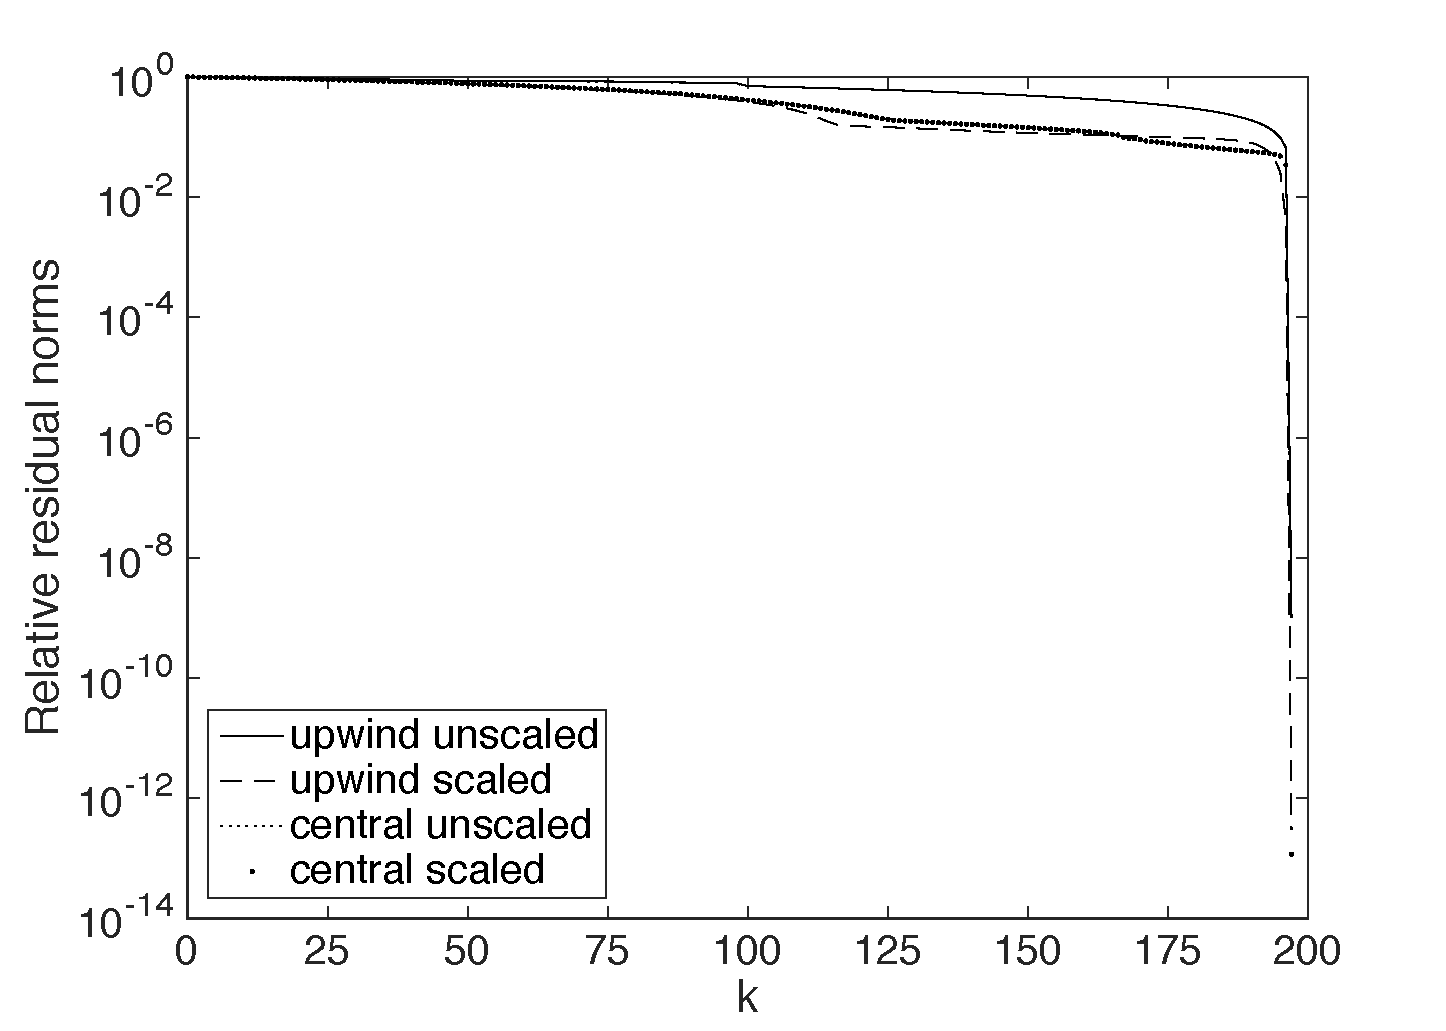
\includegraphics[width=0.95\linewidth]{figures/gmres_4_198}
% \caption{GMRES convergence for $\epsilon=10^{-4}$.}\label{fig:back:GMRES.N198.eps4}
% \end{minipage}
% %
% \begin{minipage}[t]{0.48\linewidth}
% 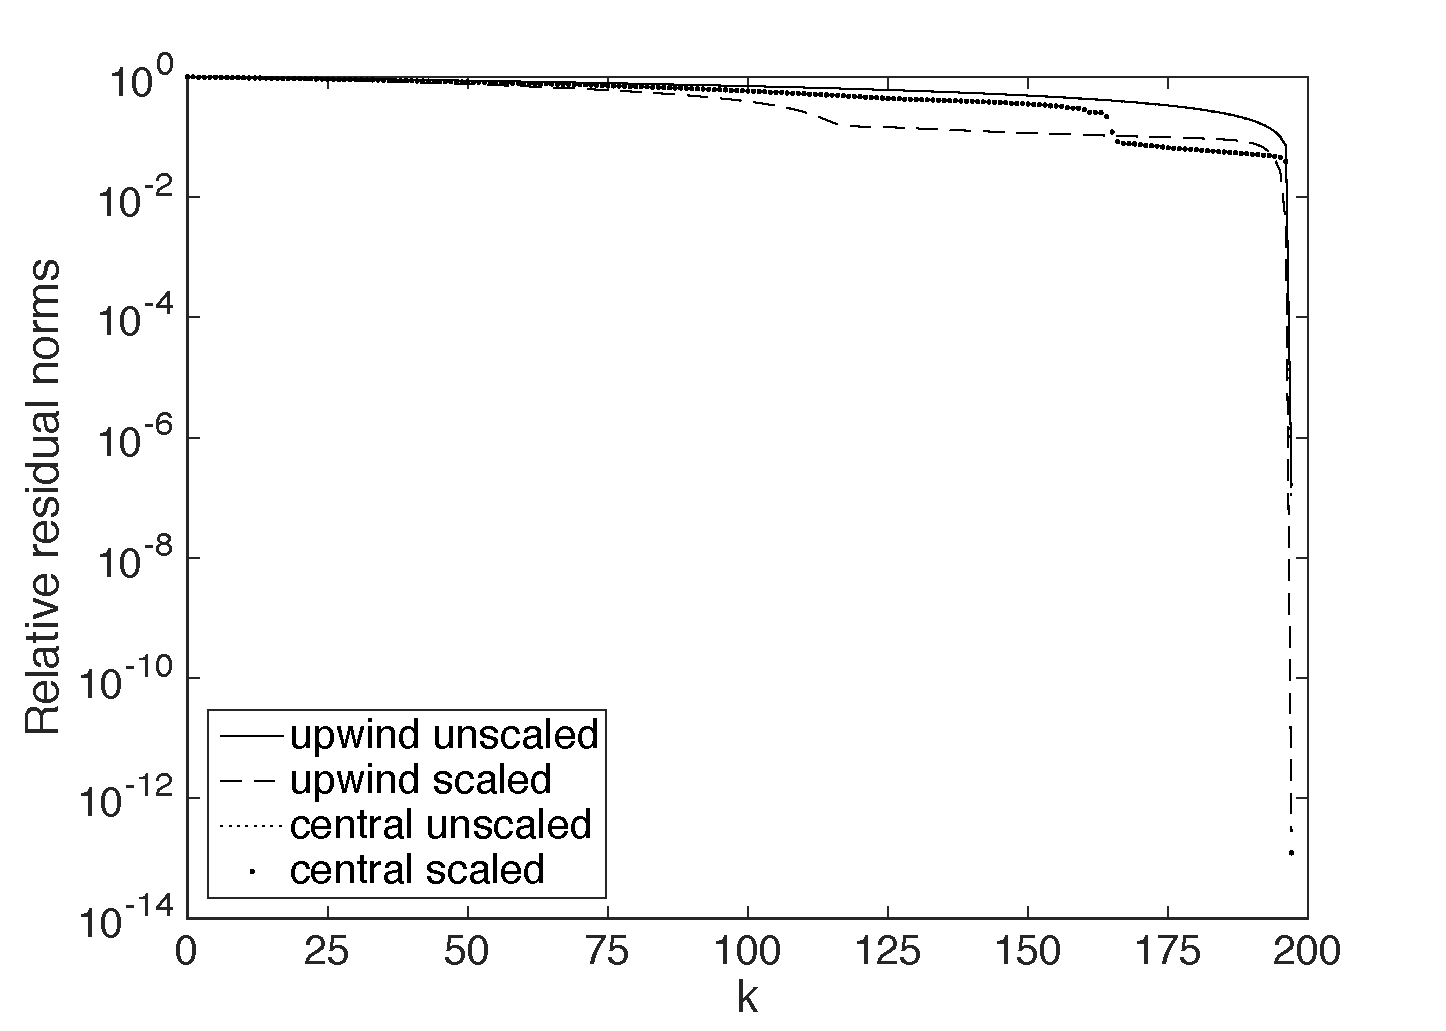
\includegraphics[width=0.95\linewidth]{figures/gmres_6_198}
% \caption{GMRES convergence for $\epsilon=10^{-6}$.}\label{fig:back:GMRES.N198.eps6}
% \end{minipage}
% \end{figure}
% %
% \begin{figure}
% \centering
% \begin{minipage}[t]{0.48\linewidth}
% 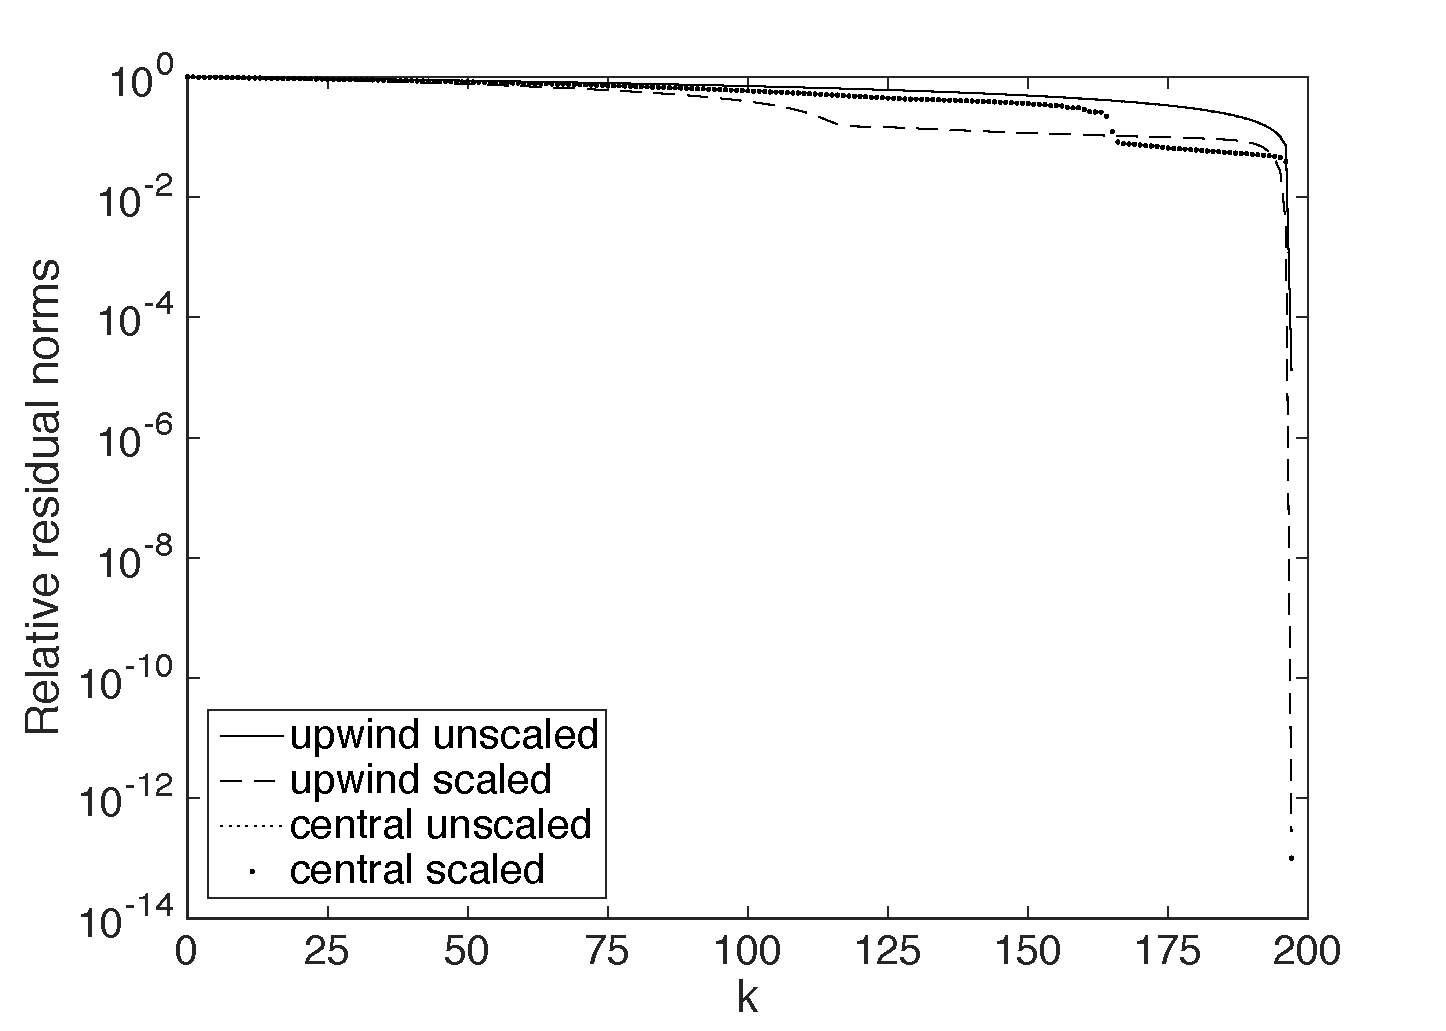
\includegraphics[width=0.95\linewidth]{figures/gmres_8_198}
% \caption{GMRES convergence for $\epsilon=10^{-8}$.}\label{fig:back:GMRES.N198.eps4}
% \end{minipage}
% \end{figure}

In the following, Figures~\ref{fig:back:GMRES.N198.eps4}--\ref{fig:back:GMRES.N198.eps8}
% \td{\textbf{fix:} recompute figures and remove scaled plots.}
illustrate that linear algebraic systems resulting from
discretizations of convection-dominated convection-diffusion problems represent
a challenge for GMRES holds for the Shishkin mesh
discretization of the model problem \eqref{eq:back:1Dbvp}. These figures show
the relative residual norms of the (unpreconditioned) GMRES method with zero
initial vector applied to $\A\u=\f$ from the Shishkin mesh discretization of
\eqref{eq:back:1Dbvp} with $\omega_x=1$, $\beta=0$, $f(x)\equiv 1$, $u_0=u_1=0$,
$N=198$, and different values of $\epsilon$. The GMRES convergence is virtually
the same for both discretizations (upwind and central differences).
 % The eigenvector conditioning does not appear to have a significant effect
% on the performance of the iterative solver.

% \begin{figure}[h!]
% \begin{minipage}[t]{0.48\linewidth}
% 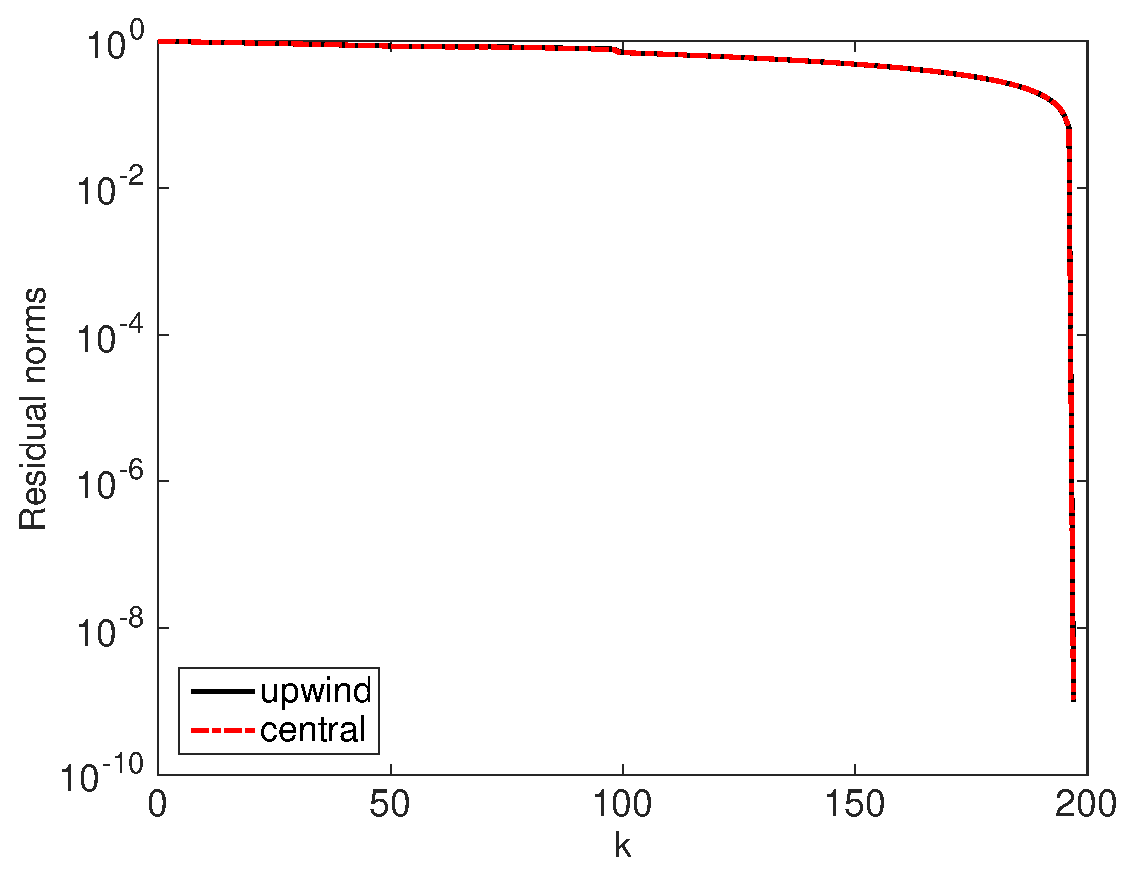
\includegraphics[width=0.95\linewidth]{figures/gmres_eps_1e-04_N_198}
% \caption{GMRES convergence for $\epsilon~=~10^{-4}$.}
% \label{fig:back:GMRES.N198.eps4}
% \end{minipage}
% %
% \begin{minipage}[t]{0.48\linewidth}
% 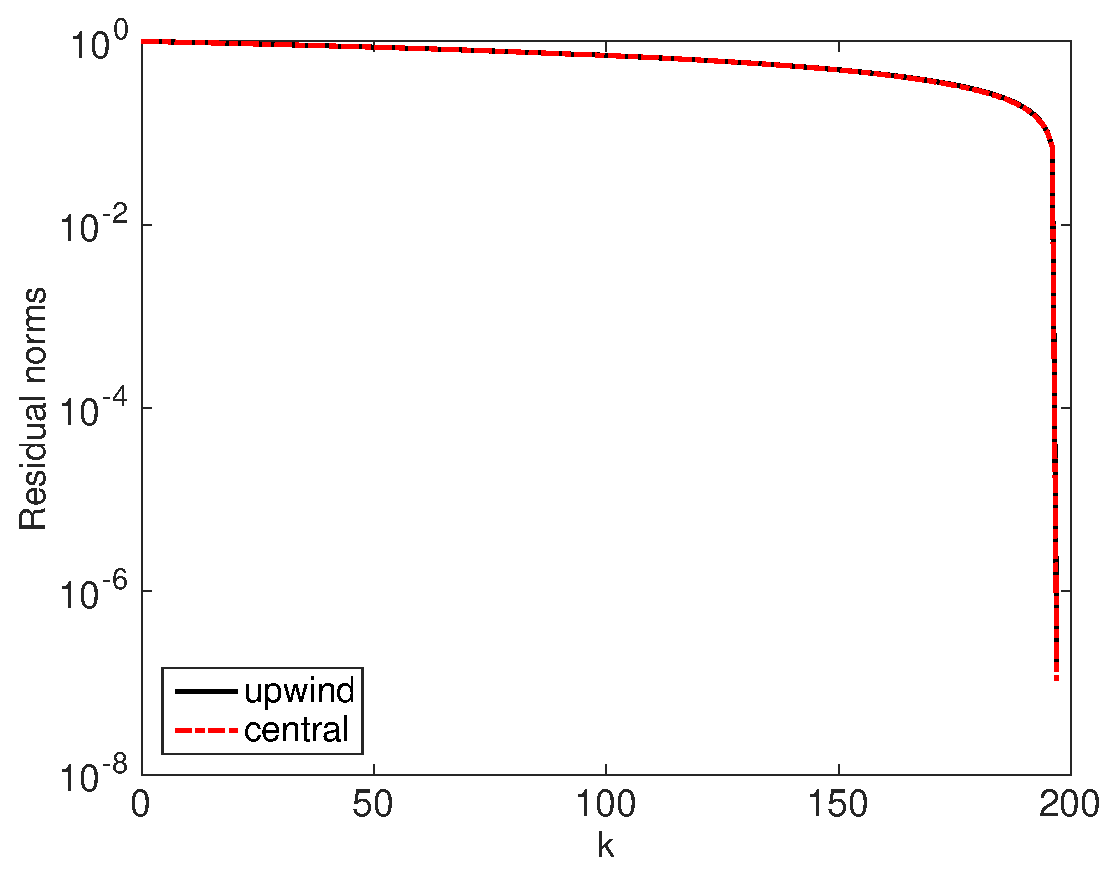
\includegraphics[width=0.95\linewidth]{figures/gmres_eps_1e-06_N_198}
% \caption{GMRES convergence for $\epsilon~=~10^{-6}$.}
% \label{fig:back:GMRES.N198.eps6}
% \end{minipage}
% %\caption{GMRES convergence for $\epsilon~=~10^{-4}$.}[left] and $\epsilon~=~10^{-6}$[right].}\label{fig:back:GMRES.N198.eps6}
% \end{figure}
%

\begin{figure}[h!]
\begin{minipage}[t]{0.48\linewidth}
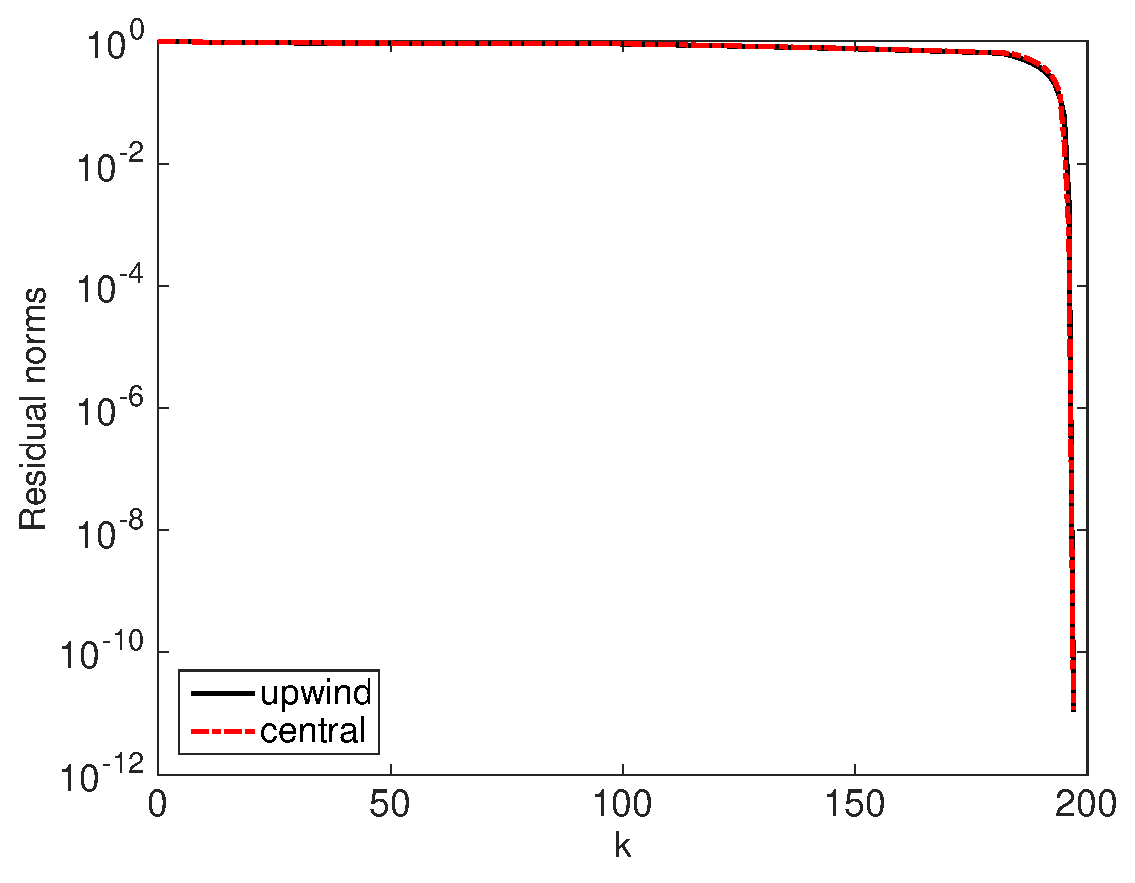
\includegraphics[width=0.98\linewidth]{figures/gmres_eps_1e-02_N_198}
%\label{fig:1D:GMRES.N198.eps4.prec}
% note: if changing to 3 figures again, it needs to be changed in two places
%\caption{Preconditioned GMRES convergence for $\epsilon=10^{-4}$.}
\end{minipage}
%
\begin{minipage}[t]{0.48\linewidth}
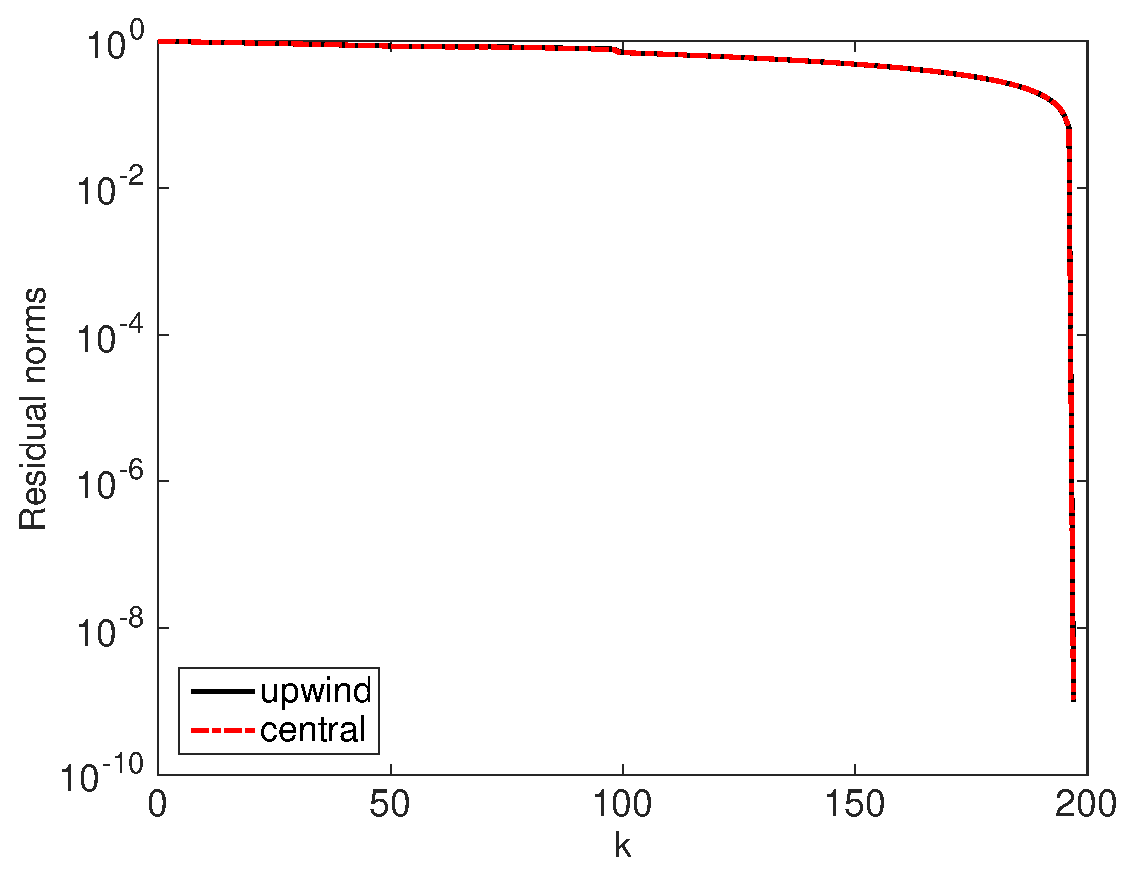
\includegraphics[width=0.98\linewidth]{figures/gmres_eps_1e-04_N_198}
\end{minipage}
\caption{GMRES convergence for $\epsilon=10^{-2}$ and $\epsilon=10^{-4}$ [r].}
\label{fig:back:GMRES.N198.eps4}
\end{figure}
%
\begin{figure}[h!]
\begin{minipage}[t]{0.48\linewidth}
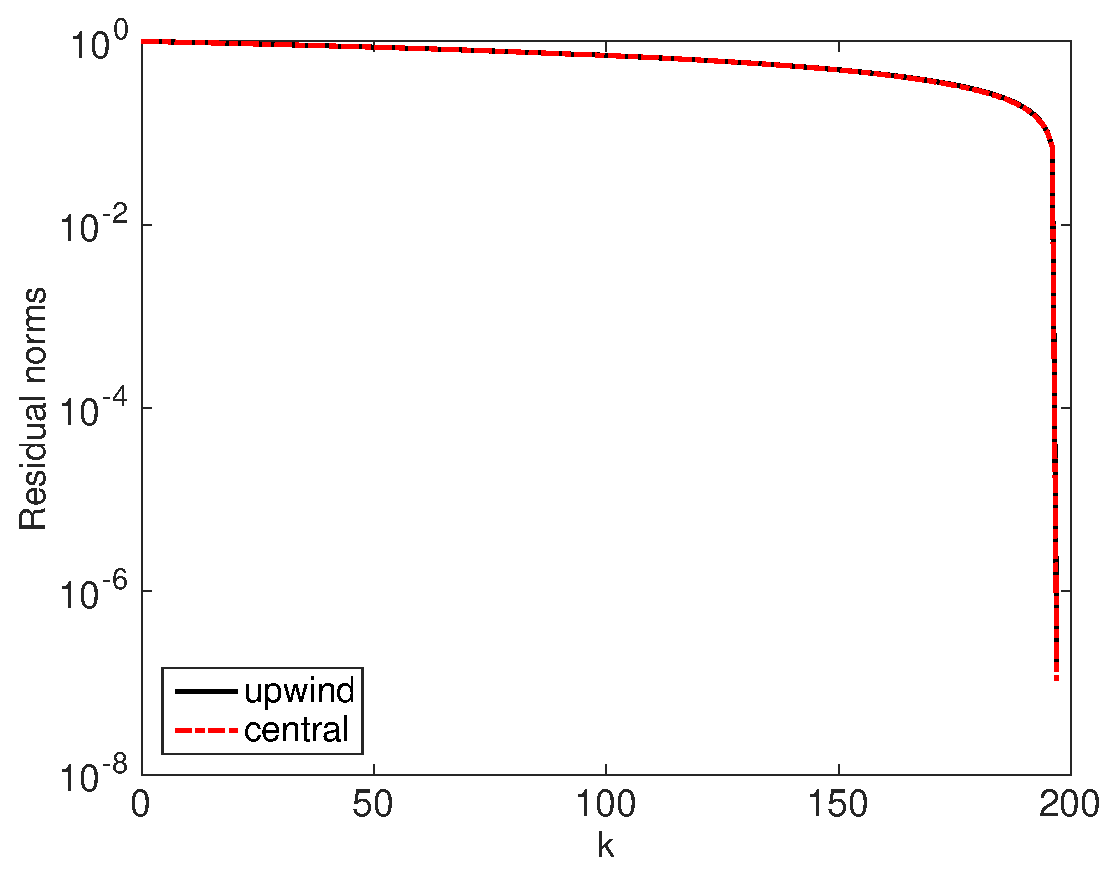
\includegraphics[width=0.98\linewidth]{figures/gmres_eps_1e-06_N_198}
%\label{fig:1D:GMRES.N198.eps4.prec}
% note: if changing to 3 figures again, it needs to be changed in two places
%\caption{Preconditioned GMRES convergence for $\epsilon=10^{-4}$.}
\end{minipage}
%
\begin{minipage}[t]{0.48\linewidth}
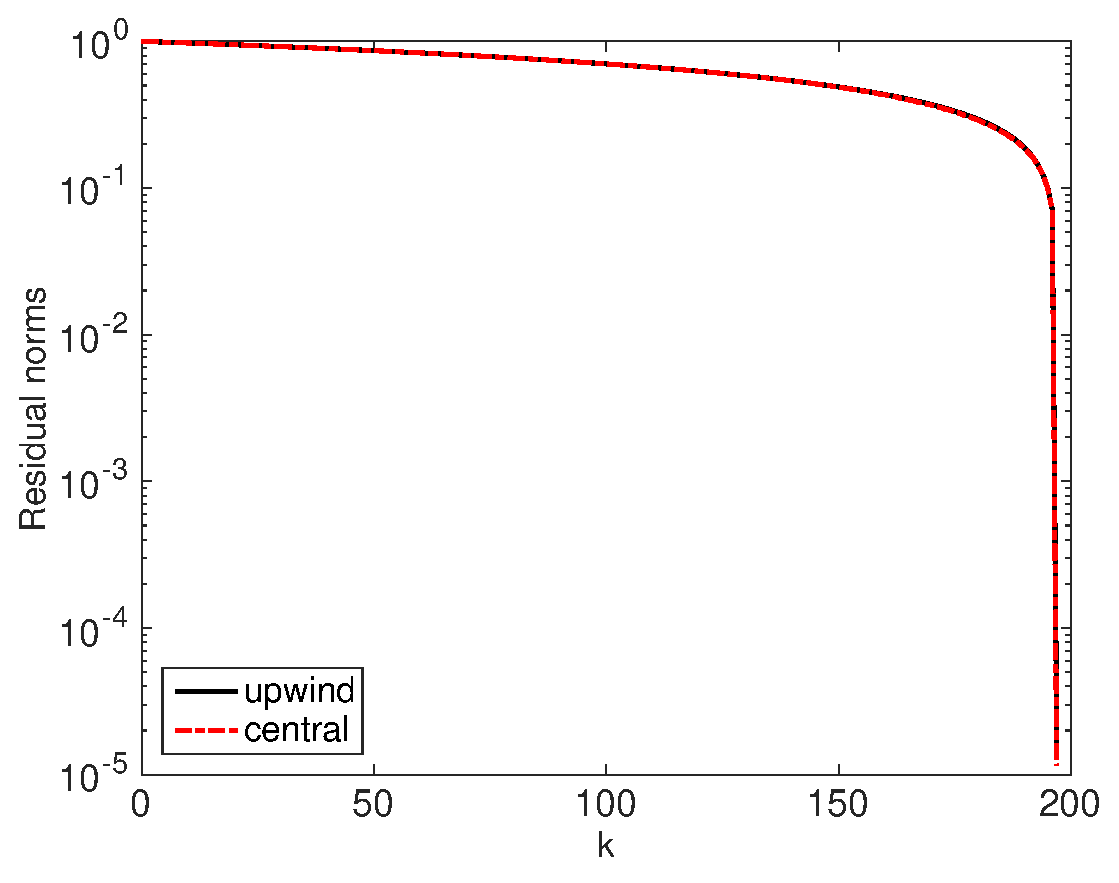
\includegraphics[width=0.98\linewidth]{figures/gmres_eps_1e-08_N_198}
\end{minipage}
\caption{Preconditioned GMRES convergence for $\epsilon=10^{-6}$ and $\epsilon=10^{-8}$ [r].}
\label{fig:back:GMRES.N198.eps8}
\end{figure}

% \begin{figure}
% \centering
% \begin{minipage}[t]{0.48\linewidth}
% 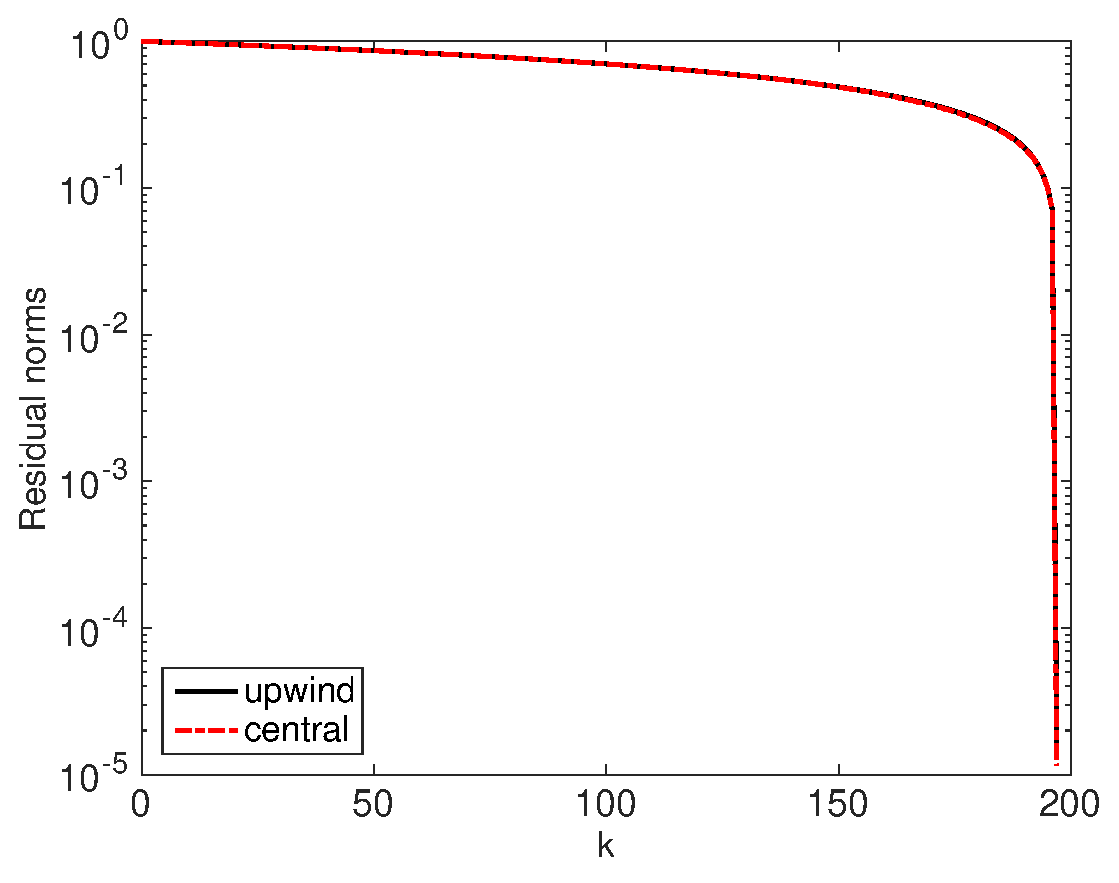
\includegraphics[width=0.95\linewidth]{figures/gmres_eps_1e-08_N_198}
% \caption{GMRES convergence for $\epsilon~=~10^{-8}$.}
% \label{fig:back:GMRES.N198.eps8}
% \end{minipage}
% \end{figure}

For the problems studied in this thesis, the eigenvector basis of the
coefficient matrix $\A$ is very badly conditioned, making the matrix highly
\emph{nonnormal}. In such cases, the use of eigenvalues and eigenvectors in an
analysis of convergence is not informative and very poorly descriptive, see for
example \cite{GreStrPta96} for an extreme case where this is true and \cite{Ern00} for an example of a convection-diffusion problem for which the eigenvalues alone give misleading information about convergence.
% \td{\textbf{add}:a good citation for this asseveration is needed (Eiermann, Ernst?)}.
% In the case of nonnormal matrices $A$, the standard approach to the GMRES
% convergence analysis is noninformative and hardly descriptive.
Such analysis use the eigendecomposition of the coefficient matrix,
$\A=\Y\D\Y^{-1}$, where $\D$ is a diagonal matrix whose elements contain the
eigenvalues $\lambda_k$ of $\A$, and is given by
\begin{align}
\|\r^{(n)}\|&=\|\Y p_n(\D) \Y^{-1}\r^{(0)}\|=\min_{p\in \pi_n}\|\Y p(\D)\Y^{-1}\r^{(0)}\|\\
&\leq\|\Y\|\|\Y^{-1}\|\|\r^{(0)}\|\min_{p \in \pi_n}\max_k|p(\lambda_k)|.
\end{align}
This result is a worst case bound that does not take into account the fact that
for some initial residuals GMRES may behave very differently than for others.
It simplifies the analysis by separating the study of GMRES convergence
behavior into optimizing the condition number of the eigenvector matrix $\Y$ and
a polynomial minimization problem over the spectrum of $\A$, but it could
potentially overestimate GMRES residuals. This is partly because, as observed
by Liesen and Strakos in \cite{LieStr03}, possible cancellations of huge
components in $\Y$ and/or $\Y^{-1}$ are artificially ignored for the sake of the
convergence analysis.

% \begin{figure}[h!]
% \centering
% 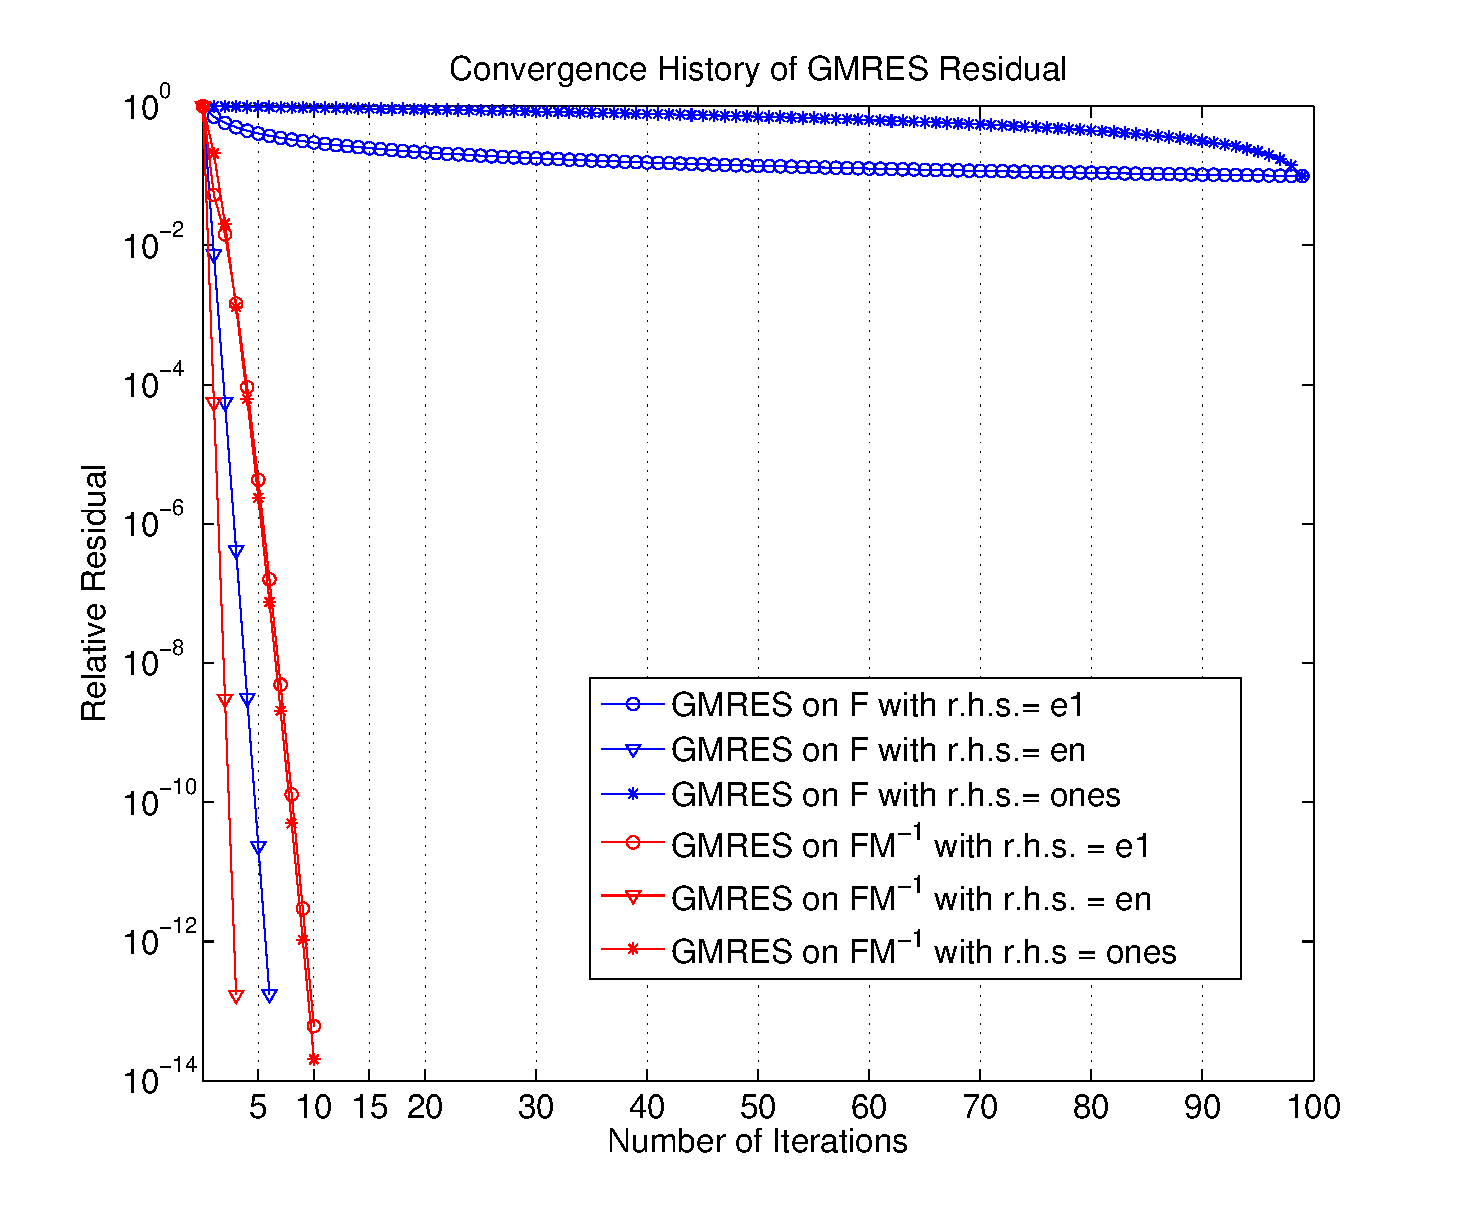
\includegraphics[scale=0.25]{figures/convergence2.eps}
% %\vspace*{-1em}
% 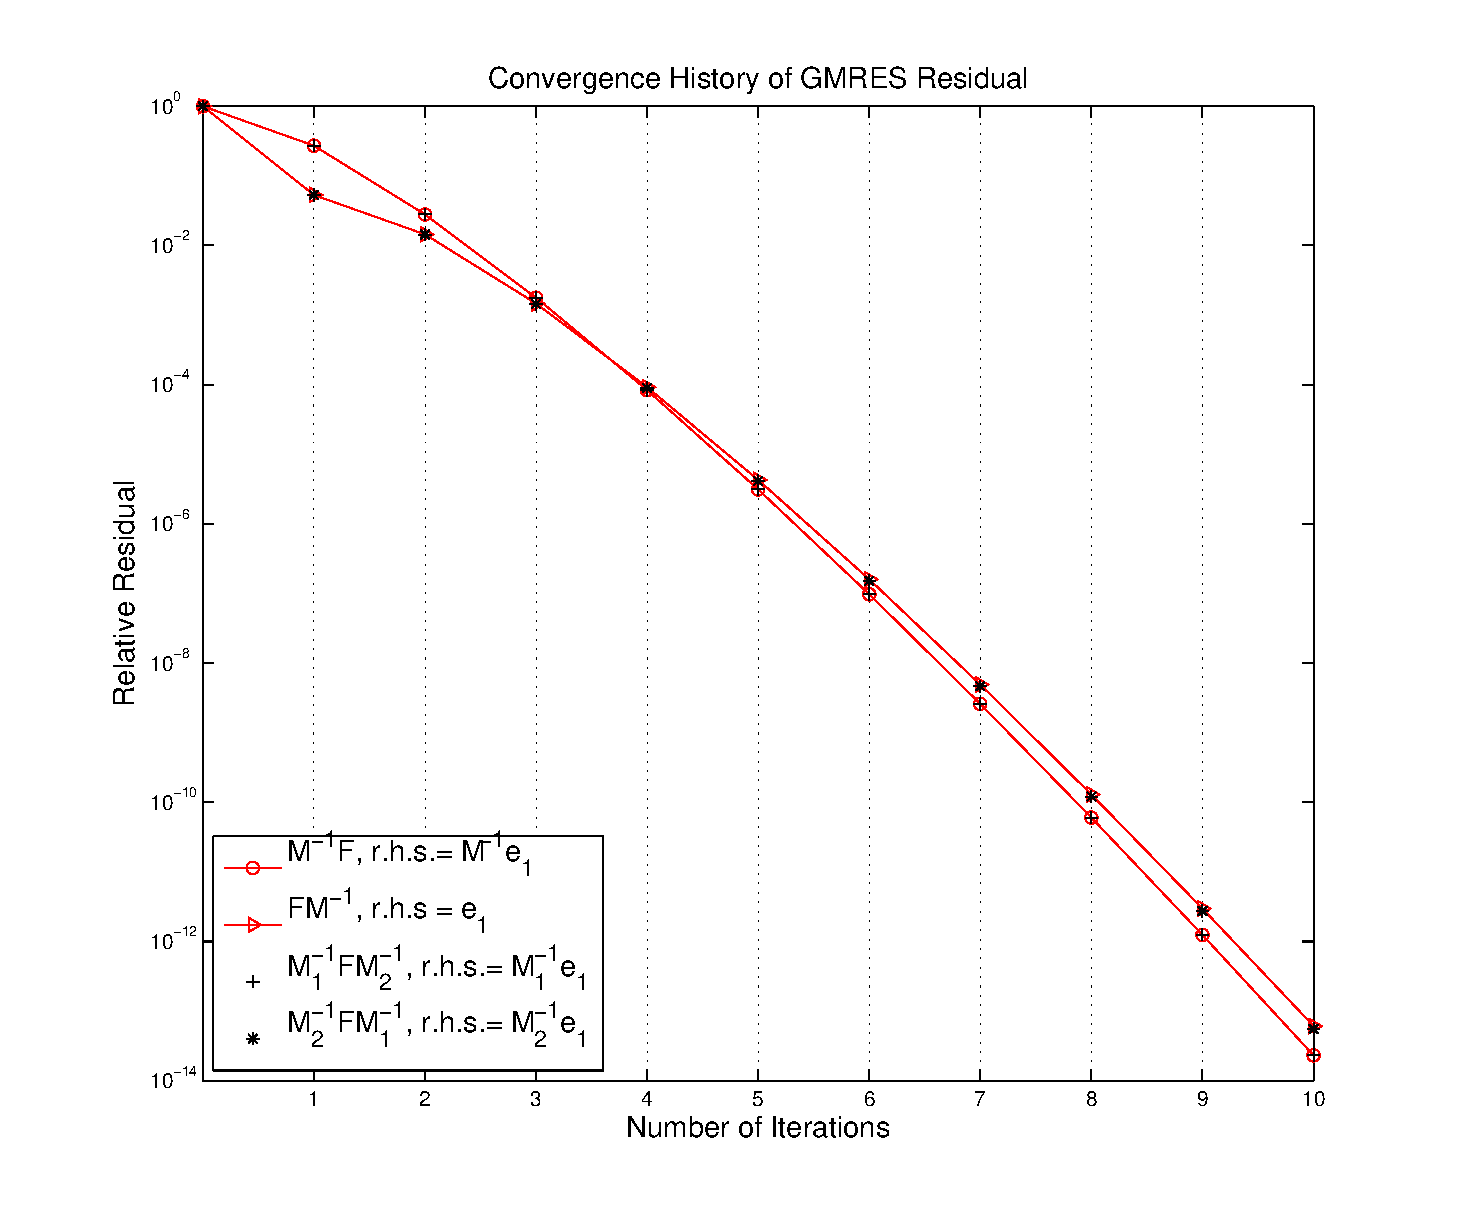
\includegraphics[scale=0.25]{figures/Convergence_e1}
% \caption{GMRES convergence history for the right-preconditioned and
% unpreconditioned systems.}
% \label{fig:back:1DConvergence}
% \end{figure}

The stagantion of GMRES for solving convection-diffusion problems of type \eqref{eq:back:1Dbvp} and \eqref{eq:back:nDbvp} shows the need to either find a preconditioning strategy to accelerate the convergence of the method or the use of a completely different solution approach to solve these types of problems. In the following we will discuss another type of solution methods which fall under the category of domain decomposition methods, which seem to be a natural solution for the types of problems studied in this thesis.


\subsection{Domain Decomposition and Schwarz Methods}
\label{back:itersolvers:DDM}

The earliest know domain decomposition method is believed to have been
discovered in 1869 by Hermann Amandus Schwarz in \cite{Sch69}. Schwarz devised
the method for elliptic equations, to establish the existence of harmonic
functions on regions with nonsmooth boundaries. Throughout the 20th century, the area of domain decomposition methods has grown extensively and a variety of methods have been introduced, both at the continuous level as well at the algebraic level; see \cite{BenFroNabSzy01} for the theory of algebraic methods and \cite{SmiBjoGro96} for a complete monograph of domain decomposition methods. Our focus in this work will fall in the algebraic case, commonly known as the multiplicative Schwarz method, however we will describe Schwarz' original idea in the following (see \cite{GanWan14} for a historical introduction to the method).
% \td{\textbf{note}: remeber to read and cite Gander's paper on Helmholtz \cite{GanZha19}}


\subsubsection{2.2.3.1. \ The Continuous Case: Schwarz's Alternating Procedure}
\label{back:itersolvers:DDM:AltSchwarz}

When the alternating Schwarz method is considered at the continuous level,
there are two main variants to be considered. The first one being the original
method invented by Schwarz in \cite{Sch69} at the end of the 19th century as a
mathematical tool for investigating the uniqueness of the solution to the
Laplace equation when it is posed on a general complex domain, and the  second
one being the parallel Schwarz method used in the general area of parallel
computing, which was introduced by Lions in the 1980's. We will briefly
describe the first one and direct the reader to the complete review paper by
Gander in \cite{Gan08} which gives a thorough analysis of Schwarz methods
over the course of time.

\begin{figure}[h!]
\centering
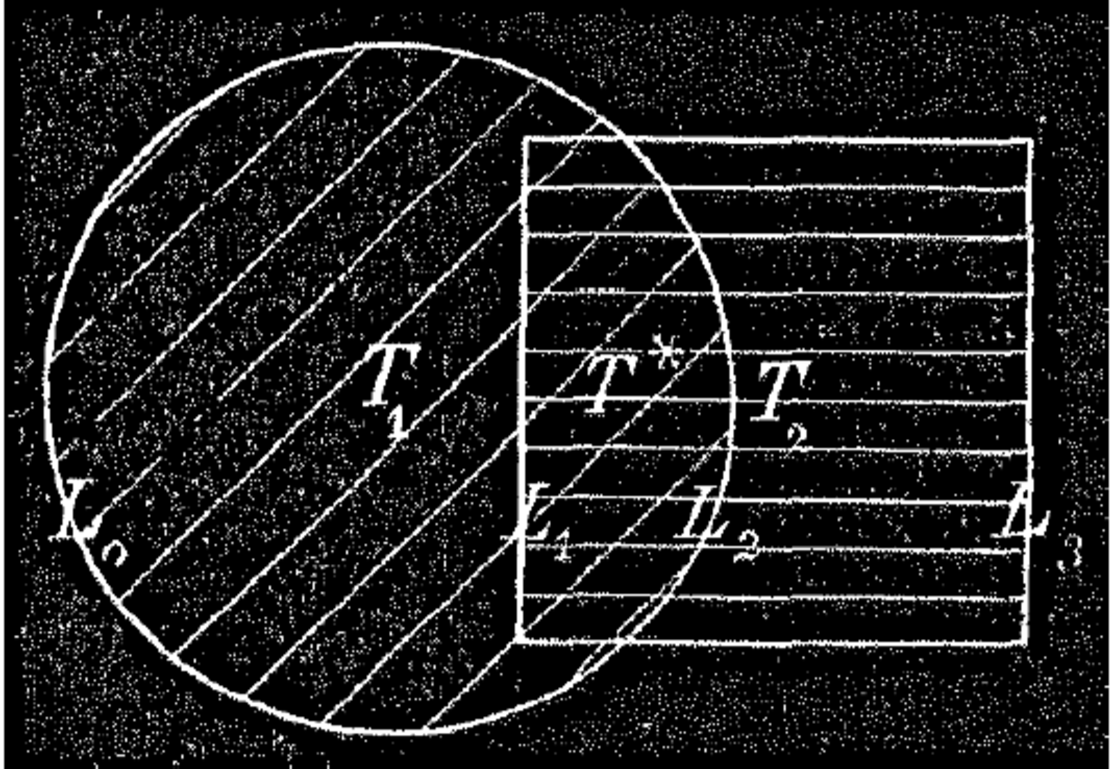
\includegraphics[scale=0.25]{figures/original_domain.pdf}
\caption{Original domain used by Schwarz consisting of a disk and a rectangle.}
\label{fig:back:orig_domain}
\end{figure}

Even though the scientific agenda at the time sought to find a proof of the uniqueness and existence of solutions for Laplace's equation posed on a general complex domain, Schwarz focused on first finding the solution on a domain that was composed of two simpler domains for which existence and uniqueness had already been proven. Figure~\ref{fig:back:orig_domain} shows the original domain used by Schwarz for his analysis, which consisted of a disk $\Omega_1$ (labeled $T_1$ in the figure) "stitched" together with a rectangle $\Omega_2$ (labeled $T_2$ in the figure). The project was to show that the following BVP
%
\begin{equation}\label{eq:back:Laplace}
\mathscr{A}u\equiv\Delta u=0,\text{ in }\Omega,\quad u=g\text{ on }\partial\Omega,
\end{equation}
%
holds for an arbitrary choice of Dirichlet boundary conditions.
Since the solutions on each subdomain were known using Fourier series,
Schwarz proposed an iterative solution scheme for the entire domain which only made use of the known solutions on the disk and the rectangle.
Providing an initial guess $u_0^2$ along $\Gamma_1\equiv\partial\Omega_1\cap\Omega_2$, the iteration computes the approximations $u_1^{n+1}$ and $u_2^{n+1}$ on each subdomain as follows:
\begin{equation}\label{eq:back:AltSchwarz}
\begin{array}{cc}
\Delta u_1^{n+1} = 0 \text{ in } \Omega_1, & \Delta u_2^{n+1} = 0 \text{ in } \Omega_2,\\
u_1^{n+1} = u_2^{n} \text{ on } \Gamma_1, & u_2^{n+1} = u_1^{n+1} \text{ on } \Gamma_2,
\end{array}
\end{equation}
where $\Gamma_2\equiv\partial\Omega_2\cap\Omega_1$ and both $u_1^{n+1}$ and $u_2^{n+1}$ satisfy the given Dirichlet conditions on the outer boundaries of each subdomain. The convergence of the previous algorithm to the solution of the problem was proven by Schwarz using a maximum principle and very loosely consisted in introducing artificial boundaries for each subdomain (given by the overlap) and using them as Dirichlet conditions for the second subdomain in order to solve each problem in an alternating fashion. For the specific proof, we direct the reader to the original paper by Schwarz in \cite{Sch69} or the survey paper \cite{Gan08}. We will next present the algebraic case, which is the main method of analysis in this thesis.

\subsubsection{2.2.3.2. \ The Discrete (Algebraic) Case: The Multiplicative Schwarz Method}
\label{back:itersolvers:DDM:MultSchwarz}

Schwarz methods have also been introduced directly at the algebraic level for
solving the linear system $\A\u=\f$, and there are several variants. We will now
describe one of them: the multiplicative Schwarz method (see \cite{BenFroNabSzy01}). In short, the method
uses restriction operators for constructing a multiplicative iteration matrix
in which each factor corresponds to a local solve in one of the subdomains.

% The multiplicative Schwarz method for solving linear algebraic systems of the
% form \eqref{eq:linsys} uses restriction operators for constructing a
% multiplicative iteration matrix, where each factor corresponds to a local solve
% in one of the subdomains $\Omega_1$ and $\Omega_2$.

\begin{figure}[h]
\centering
% \begin{tikzpicture}
%  % \tikzset{
%  %   elps/.style 2 args={draw, ellipse,minimum width=#1, minimum height=#2},
%  %   node distance=1.8 cm,
%  %   font=\footnotesize,
%  %   >=latex,
%  %   bullet/.style = {circle, inner sep=1pt, fill}
%  % }
%     \draw [gray!50]  (0,0) -- (1,1) -- (3,1) -- (5,0.9)  -- (5,-1) -- cycle;
%     \draw [red] plot [smooth cycle] coordinates {(0,0) (1,1) (3,1) (5,1) (5,-1)};
%     % \node(a)[elps={3cm}{1.5cm},label={below:$\Omega$}]
%     %    [path picture=\ppfill{white}{white}]{};
%     \node at (-1.0,0.2) {$\Omega_{1}$};
%     \node at (0.1,0.35) {$\Gamma_{12}$};
%     \node at (1.0,-0.2) {$\Omega_{2}$};%
%
% \end{tikzpicture}
\begin{turn}{90}
\begin{tikzpicture}[scale=0.06]
\draw (0, 0) .. controls (5.18756, -26.8353) and (60.36073, -18.40036)
   .. (60, 40) .. controls (59.87714, 59.889) and (57.33896, 81.64203)
   .. (40, 90) .. controls (22.39987, 98.48387) and (4.72404, 84.46368)
   .. (10, 70) .. controls (13.38637, 60.7165) and (26.35591, 59.1351)
   .. (30, 50) .. controls (39.19409, 26.95198) and (-4.10555, 21.23804)
   .. (0, 0);
\draw (30.7,40.0) -- (60.0,40.0);
\begin{turn}{-90}
\node at (-10,26) {$\Omega_{2}$};
\node at (-30,45) {$\Gamma_{12}$};
\node at (-75,26) {$\Omega_{1}$};
\end{turn}
\end{tikzpicture}
\end{turn}
\vspace*{-5cm}
\caption{Decomposition of a domain $\Omega$ into two local subdomains $\Omega_1$ and $\Omega_2$ with interface boundary $\Gamma_{12}$.}
\label{fig:back:2DSchwarzdomain}
\end{figure}

% \begin{figure}[h]
% \centering
% \begin{tikzpicture}
%  \tikzset{
%    elps/.style 2 args={draw, ellipse,minimum width=#1, minimum height=#2},
%    node distance=1.8 cm,
%    font=\footnotesize,
%    >=latex,
%    bullet/.style = {circle, inner sep=1pt, fill}
%  }
%
%     \node(a)[elps={3cm}{1.5cm},label={below:$\Omega$}]
%        [path picture=\ppfill{white}{white}]{};
%     \node at (-1.0,0.2) {$\Omega_{1}$};
%     \node at (0.1,0.35) {$\Gamma_{12}$};
%     \node at (1.0,-0.2) {$\Omega_{2}$};%
%
% \end{tikzpicture}
% \caption{Decomposition of a domain $\Omega$ into two local subdomains $\Omega_1$ and %$\Omega_2$ with interface boundary $\Gamma_{12}$.}
% \label{fig:domain}
% \end{figure}

Just like the continuous domain is partitioned into subdomains, the unknowns in the vector $\u$ need to be subdivided into corresponding subsets, possibly overlapping each other. Without loss of generality, and referring to Figure~\ref{fig:back:2DSchwarzdomain}, %\td{\textbf{fix:} write a TIkz figure with a generic domain},
we consider one domain, $\Omega$, subdivided into two contiguous local subdomains, $\Omega_1$ and $\Omega_2$, by one interface boundary $\Gamma_{12}$. The only assumption we make is that in each of the local subdomains we have the same number of unknowns. This assumption is made for simplicity of the following exposition. Extensions to other block sizes and several subdomains are certainly possible, but would require even more technicalities. In this context, the restriction operators can be written as
% \td{\textbf{write}: mention that the analysis can be extended to any number of domains and therefore we will have as many number of projectors}
%
$$\R_1\equiv \left[\I_{n}\quad 0 \right]\quad\mbox{and}\quad \R_2\equiv \left[0\quad  \I_{n} \right],$$
%
both of size $n\times (N-1)$.
%\td{\textbf{fix}: the notation $\I_{\text{size}}$ is not used after this point - change the rest so that it does. To be consistent we also need a $\mathbf{0}$ to represent the array of zeros too}
Therefore the operation $\R_1\u$ yields the
unknowns in the first subset while $\R_2\u$ delivers the unknowns of the second
subset (subdomain). The corresponding unknowns in the matrix $\A$ can be
obtained using the same restriction operators and thus, the restrictions of the
matrix $\A$ in $\A\u=\f$ to the two subdomains are given by the two $n\times n$
matrices
%
\begin{equation}\label{eq:back:local_prob}
\matA_1 \equiv \R_1\A\R_1^T \equiv
\left[\begin{array}{cc}
\matAH &\entryvE  \e_{m }\\
\entryzW \e_{m}^T& \entryzC
\end{array}\right]
\quad\mbox{and}\quad
\matA_2\equiv \R_2\A\R_2^T\equiv
\left[\begin{array}{cc}
\entryzC &\entryzE \e_{1}^T\\
\entrywW \e_{1}& \matAh
\end{array}\right],
\end{equation}
%
where $m\equiv n-1$, and $\e_1,\e_m\in {\mathbb R}^m$. In the following, the
unit basis vectors $e_j$ are always considered to be of appropriate length,
which for simplicity is sometimes not explicitly stated. Note that
$\matAH, \matAh\in \mathbb{R}^{m\times m}$ are tridiagonal Toeplitz matrices.
The matrices corresponding to the solves on the two domains then are given by
%
\begin{equation}\label{eq:back:Pi}
\P_i\equiv \R_i^T\A_i^{-1}\R_i\A,\quad i=1,2.
\end{equation}
%
It is easy to see that $\P_i^2=\P_i$, i.e., that these matrices are projections.
Note also that since $\P_i$ is not symmetric, we have for the 2-norm,
that $\|\I-\P_i\|_2 = \|\P_i\|_2 > 1$; see, e.g., \cite{Szy06}. Using the
complimentary projections
%
$$\Q_i\equiv \I-\P_i\;\in\;\mathbb{F}^{(N-1)\times (M-1)},\quad i=1,2,$$
%
we define the multiplicative Schwarz iteration matrices
%
\begin{equation}\label{eq:back:Tij}
\T_{12}\equiv \Q_2\Q_1\quad\mbox{and}\quad \T_{21}\equiv \Q_1\Q_2.
\end{equation}
%
Thus, $\T_{ij}$ corresponds to first solving on $\Omega_i$, and then on
$\Omega_j$. Both iteration matrices will be analyzed below.

Starting with an initial vector $\u^{(0)}\in{\mathbb R}^{N(2m+ 1)}$,
%$\hat{\u}^{(0)}=[\hat{u}_1^{(0)},\hat{u}_2^{(0)},\ldots,\hat{u}_{2m+1}^{(0)}]\in{\mathbb R}^{N(2m+ 1)}$
the multiplicative Schwarz method is defined by
%
\begin{equation}\label{eq:back:schwarz}
\u^{(k+1)}=\T_{ij} \u^{(k)}+\v, \quad k=0,1,2,\dots,
\end{equation}
%
where $\T_{ij}=\T_{12}$ or $\T_{ij}=\T_{21}$, and the vector
$\v\in {\mathbb R}^{N-1}$ is defined to make the method consistent.
For the iteration matrix $\T=\T_{ij}$ the consistency condition
$\u=\T_{ij}\u+\v$ yields
$$
\v = (\I-\T_{ij})\u = (\P_i+\P_j-\P_j\P_i)\u,
$$
which is (easily) computable since
$$
\P_i\u=\R_i^{\Tr}\A_i^{-1}\R_i\A\u=\R_i^{\Tr}\A_i^{-1}\R_i\f,\quad i=1,2.
$$

The error of the multiplicative Schwarz iteration~\eqref{eq:back:schwarz} is
given by
\begin{equation}\label{eq:back:schwarz_err}
\e^{(k+1)}=\u-\u^{(k+1)}=(\T_{ij}\u + \v)- (\T_{ij} \u^{(k)}+\v)=\T_{ij} \e^{(k)},
\quad k=0,1,2,\dots,
\end{equation}
and hence $\e^{(k+1)}=\T_{ij}^{k+1} \e^{(0)}$ by induction.
For any consistent norm $\|\cdot\|$, we therefore have the error bound
%
\begin{equation}\label{eq:back:error}
\|\e^{(k+1)}\|\leq \|\T_{ij}^{k+1}\|\,\|\e^{(0)}\|.
%\leq \|T_{ij}\|^{k+1}\,\|e^{(0)}\|.
\end{equation}
%
Our main goal on the following chapters of this work is the derivation of
quantitative convergence bounds for the error of the multiplicative Schwarz method, where we consider both
$\T_{ij}=\T_{12}$ and $\T_{ij}=\T_{21}$.
%$\T_{12}~=~(\I~-~\P_2)(\I~-~\P_1)$ and $\T_{21}~=~(\I~-~\P_1)(\I~-~\P_2)$.

% We point out that the analysis of the multiplicative Schwarz method
% in the following sections uses the unscaled linear algebraic system with $A$
% as in~\eqref{eq:back:matrix} having the entries~\eqref{eq:back:upwind}
% or~\eqref{eq:back:central}. In Section~\ref{ss:scaling} we explain why this
% analysis also applies to suitably scaled linear algebraic systems, and in
% particular to the scaling suggested by Roos in~\cite{Roo96}.


\fi % end of if statement regarding content shown


%\chapter{Solution of Discretized 1D Convection-Diffusion Problems}
\chapter{Convergence of the Multiplicative Schwarz Method for Shihskin Mesh Discretizations of One-dimensional Convection-Diffusion Problems}
\chaptermark{Convergence of the Multiplicative Schwarz Method for 1D Shihskin Problems}
\label{ch:1D}
\ifnum\switch=1
% -----------------------------------------------------------------------------
% ------------------------------ Extended ToC ---------------------------------
% -----------------------------------------------------------------------------
%data mostly gotten from: PHD_Docs/LaTeX/Shishkin/ETNA17001_revised/Ech.Lie.Szy.Tic.17_rev.tex
Parts of this chapter have already been published in:
\begin{enumerate}
\item[\cite{EchLieSzyTic18}] \underline{C.~Echeverr{\'\i}a}, J.~Liesen, D.~B.~Szyld, and P.~Tich{\'y}, \textbf{Convergence of the multiplicative Schwarz method for singularly perturbed convection-diffusion problems discretized on a Shishkin mesh}, Electron. Trans. Numer. Anal., 48 (2018), pp. 40--62.
\end{enumerate}


\section{Introduction}
This section is based on the following references: \cite{EchLieSzyTic18, GriDolSil15}.
\paragraph{Keywords:} Bounds on Infinity norm, solving linear systems with mSm,


\section{The Model Problem and its Shishkin Mesh Discretization}
This section is based on the following references: \cite{GriDolSil15, Lin10, RooStyTob08, Sty05}.


\section{Convergence Bounds for the Multiplicative Schwarz Method}
This section is based on the following reference: \cite{EchLieSzyTic18}.


\subsection{Bounds for the Upwind Difference Scheme}


\subsection{Bounds for the Central Difference Scheme}


\section{The Stagnation of GMRES}
This section is based on the following references: \cite{Gal13, GolVan13, HorJoh12, Saa03}.
\paragraph{Keywords:} Eigenvalue analysis is useless


\section{Shishkin-Schwarz Preconditioning}
This section is based on the following references: \cite{EchLieSzyTic18, KahKamPhi07}.


\section{Flow-Following Preconditioning}
This section is based on the following references: \cite{EchGarSet19, ElmSilWat14}.
\paragraph{Keywords:} The name flow following comes from \cite{AndKop96}


\section{Numerical Experiments}
This section is based on the following references: \cite{ElmSilWat14}.

\subsection{Upwind Finite Differences}
This section is based on the following references: \cite{EchLieSzyTic18, Smi85}.


\subsection{Central Finite Differences}
This section is based on the following references: \cite{EchLieSzyTic18, Smi85}.


\else
% -----------------------------------------------------------------------------
% --------------------------- Content of Chapter ------------------------------
% -----------------------------------------------------------------------------

Parts of this chapter have already been published in:
\vspace*{0.3cm}
%
\begin{enumerate}
\item[\cite{EchLieSzyTic18}] \underline{C.~Echeverr{\'\i}a}, J.~Liesen, D.~B.~Szyld, and P.~Tich{\'y}, \textbf{Convergence of the multiplicative Schwarz method for singularly perturbed convection-diffusion problems discretized on a Shishkin mesh}, Electron. Trans. Numer. Anal., 48 (2018), pp. 40--62.
\end{enumerate}
%
\vspace*{0.25cm}
%
\section{Introduction}
\label{1D:intro}

In this chapter we study the convergence behavior of the multiplicative
Schwarz method when it is used to solve linear systems of the form
%
\begin{equation}\label{eq:1D:linsys}
\mathbf{A}\mathbf{u}=\mathbf{f},
\end{equation}
%
where the coefficient matrix is obtained from finite difference discretizations
of the following one-dimensional constant coefficient convection-diffusion BVP
with Dirichlet boundary conditions posed on a Shishkin mesh:
\begin{equation}\label{eq:1D:bvp}
\begin{cases}
%-\epsilon  u''(x) + \omega u'(x)+\beta u(x) = f(x), & \text{in}\; (0,1)\\
-\epsilon\frac{\partial^2 u(x)}{\partial x^2}+\omega_x \frac{\partial u(x)}{\partial x} + \beta u(x)=f(x), & \text{in}\; (0,1)\\
\hspace{0.8cm} u(0)=g_0,\;\text{ and }\;u(1)=g_1, &
\end{cases}
% \begin{cases}
% %\mathscr{A}u(x)\equiv
% -\epsilon  u''(x) + \omega_x u'(x)+\beta u(x) = f(x), &  0<x<1,\\
%             \qquad\;\;u(0)=g_0,\;\;u(1)=g_1. &
% \end{cases}
\end{equation}
%
We assume $\omega_x\gg \epsilon >0$ and $\beta\geq 0$ and that the parameters
of the problem, i.e., $\epsilon,\omega_x,\beta,f,g_0,$ and $g_1$, are chosen
so that the solution $u(x)$ has one boundary layer close to the point $x=1$.
We resolve the boundary layer using a finite difference discretization on a
one-dimensional Shishkin mesh with transition point close to $x=1$ and
consider two different schemes on the mesh: upwind and central differences.

After the discretization process, the structure of the coefficient matrix,
$\A$ in \eqref{eq:1D:linsys}, takes the form:
%
\begin{equation}\label{eq:1D:struct}
\A=\left[
  \begin{array}{c|c|c}
     \matAH & \entryvE &          \\ \hline
  \entryzW  & \entryzC & \entryzE \\ \hline
            & \entrywW & \matAh
  \end{array}
\right],%\;\in\;{\mathbb R}^{(N-1)\times (N-1)}.
\end{equation}
where the matrices $\matAH$ and $\matAh$ %\;\in\;{\mathbb R}^{(n-1)\times (n-1)}$
are given by:
\begin{equation}
\matAH = \text{tridiag}(\entryvW, \entryvC, \entryvE),\quad \text{and} \quad
\matAh = \text{tridiag}(\entrywW, \entrywC, \entrywE),
\end{equation}
%
and $\entryvW, \entryvC, \entryvE,\entrywW, \entrywC, \entrywE\in\Re$. In turn,
the structure of the coefficient matrix \eqref{eq:1D:struct} induces a very
special rank-one structure of the iteration matrices $\T_{ij}$, defined in
\eqref{eq:back:Tij} and used in the multiplicative Schwarz method. Using the
resulting algebraic structure of the iteration matrices, we derive bounds on
the infinity norm of the error produced by the method at each iteration step.
Unlike asymptotic convergence results based on bounding the spectral radius of
the iteration matrix, our results apply to the transient rather than the
asymptotic behavior and thus our error bounds are valid from the first step of
the multiplicative Schwarz iterations.

For linear systems obtained from the upwind scheme we prove rapid convergence
of the  multiplicative Schwarz iteration for all relevant parameters in the
problem. The analysis of the central difference scheme is more complicated,
since some of the submatrices that occur in this case are not only
nonsymmetric, but also fail to be $M$-matrices. This reminds of the analysis
in~\cite{AndKop96}, which showed that in this case the difference scheme
itself does not satisfy a discrete maximum principle. Nevertheless, we can
prove the convergence of the multiplicative Schwarz method for problems
discretized by central differences on a Shishkin mesh under the assumption
that the number of discretization points in each of the local subdomains is
even. If this assumption is not satisfied, then the method may diverge, which
we also explain in our analysis.

Furthermore, we study the convergence of the preconditioned GMRES method when
the multiplicatvie Schwarz method is used as a preconditioner and show that the
low-rank structure of the iteration matrices $\T_{ij}$ is enough to prove
convergence of the preconditioned GMRES method independently of the
perturbation parameter~$\epsilon$.
%We also present the ideas of \emph{Flow-Following} preconditioners and provide an analysis of convergence of GMRES when these type of preconditioning is used and show that they are efficient in getting rid of the well-known stagnation of GMRES (see \cite{LieStr03}) present when used to solve linear systems with the
%unpreconditioned system.

The chapter is organized as follows. We immediately begin by presenting
the convergence analysis of the multiplicative Schwarz method in
Section~\ref{1D:bounds}; first for the upwind scheme and
then for the central difference scheme. Background material including the
Shishkin mesh discretization of the one-dimensional model problem is specified
in previous chapters (see Chapter~\ref{ch:back}). In Section~\ref{1D:ShishScwarzPrecon} we discuss the performance of GMRES when
preconditioned with the multiplicative Schwarz method.
%In Section~\ref{1D:FlowFollowPrecon} we present an analysis of the convergence
%of GMRES when a second type of preconditioners, \emph{Flow-Following preconditioners}, are used.
Numerical examples are shown in Section~\ref{1D:NumericsA}.

%\hfill
%\newpage

% \section{The Shishkin Mesh Discretization of the Model Problem}
% \label{1D:ModProb}
%
% We consider the one-dimensional convection-diffusion boundary value
% problem with constant coefficients and Dirichlet boundary conditions given by
% \eqref{eq:1D:bvp} and proceed to apply the finite difference procedure
% described in Section \ref{back:convdiff:findiff} on the one-dimensional
% Shishkin mesh presented in Section \ref{back:convdiff:shihs1D} and shown in
% Figure \ref{fig:back:shmesh1D}.
%
% % The first derivative of $u$ at the point $x_i$ approximated by the standard
% % upwind finite difference operator (see Section \ref{back:convdiff:findiff}) is
% % given by
% % \begin{equation*}
% % %\frac{\partial u(x_i)}{\partial x}
% % u'(x_i)\approx
% % %(\Delta x)^{-1}D^{-}_{x} u_{i}^D = (\Delta x)^{-1}(u_{i}^D-u_{i-1}^{N})=
% % \frac{u_i^D-u_{i-1}^{N}}{h_i},
% % \end{equation*}
% % and using the central finite difference operator we obtain
% % \begin{equation*}\label{eq:firstcen}
% % %\frac{\partial u(x_i)}{\partial x}
% % u'(x_i)\approx %(\Delta x)^{-1} D^{0}_{x} u_{i}^D =(\Delta x)^{-1}(u_{i+1}^D-u_{i-1}^{N})=
% % \frac{u_{i+1}^D-u_{i-1}^{N}}{(h_i+h_{i+1})}.
% % \end{equation*}
% % The second derivative can be approximated by
% % \begin{equation*}
% % %\frac{\partial u(x_i)}{\partial x^2}
% % u''(x_i)\approx %\delta^{2}_{x} u_{i}^D\; =\;
% % \frac{2 u_{i-1}^D}{(h_{i} + h_{i+1}) h_{i+1}}- \frac{2u_{i}^D}{h_{i} h_{i+1}} + \frac{2 u_{i+1}^D}{(h_{i} + h_{i+1}) h_{i+1}}.
% % \end{equation*}
% Applying the discrete operators given in Table~\ref{tab:back:findiff} on the
% nodes of the Shishkin mesh, where $h_i=H_x$ for $i=1,\ldots,n$ and $h_i=h_{x}$
% for $i=n+1,\ldots,N-1$, we obtain for the upwind scheme:
% \begin{equation}
% \Delta^{-}_{x} u_{i}^D\; =\;
% \begin{cases}
% \frac{1}{H_x}\left(u_{i}^D-u_{i-1}^D\right) & \mbox{for}\;\; i=1,\ldots, n, \\
% \frac{1}{h_x}\left(u_{i}^D-u_{i-1}^D\right) & \mbox{for}\;\; i={n+1},\ldots, N-1,
% \end{cases}
% \end{equation}
% and for the central finite difference scheme we obtain
% \begin{equation}
% \Delta^{0}_{x} u_{i}^D\; =\;
% \begin{cases}
% \frac{1}{2H_x}\left(u_{i+1}^D-u_{i-1}^D\right) &
% \mbox{for}\;\; i=1,\ldots, {n-1},\\
% \frac{1}{h_x+H_x}\left(u_{i+1}^D-u_{i-1}^D\right)  &
% \mbox{for}\;\; i=n,\\
% \frac{1}{2h_x}\left(u_{i+1}^D-u_{i-1}^D\right)  &
% \mbox{for}\;\;i={n+1},\ldots, {N-1}.
% \end{cases}
% \end{equation}
% For the second derivatives, we obtain
% \begin{equation}\label{eq:back:second}
% \delta^{2}_{x} u_{i}^D\; =\;
% \begin{cases}
% \frac{1}{H_x^2}\left(u_{i-1}^D - 2u_{i}^D + u_{i+1}^D\right) &
% \mbox{for}\;\; i=1,\ldots, {n-1},\\
% \frac{2u_{i-1}^D}{(H_x+h_x)H_x} - \frac{2u_{i}^D}{H_xh_x} + \frac{2u_{i+1}^D}{(H_x+h_x)h_x} &
% \mbox{for}\;\; i=n,\\
% \frac{1}{h_x^2}\left(u_{i-1}^D - 2u_{i}^D + u_{i+1}^D\right) &
% \mbox{for}\;\;i={n+1},\ldots, {N-1}.
% \end{cases}
% \end{equation}
%
% % Considering the homogeneous boundary conditions $u_0 = u_1 = 0$ and letting
% % $\omega(x)=\omega>0$, and $\beta(x) = \beta>0$ be constant along the domain,
% % the finite difference scheme applied to the differential equation in \eqref{eq:1D:bvp} on
% % the Shishkin mesh is then given~by
% % \begin{equation}\label{eq:1DdiscrOp}
% % %\Au^D_m\equiv
% % -\epsilon \delta_x^2 u^D_i + \omega \Delta^{-/0}_{x}u^D_i +\beta_i u^D_i= f_i,\quad i=1,2,\ldots,N-1\equiv M.
% % \end{equation}
% Thus, by including the boundary conditions and letting $\omega(x)=\omega_x>0$
% and $\beta(x) = \beta > 0$ be constant along the domain, the finite difference
% scheme applied to the continuous problem \eqref{eq:1D:bvp} results in the
% discrete version of our model problem:
% % consists of the
% % following discretization of the one-dimensional convection-diffusion boundary
% % value problem with constant coefficients and Dirichlet boundary conditions:
% %
% \begin{equation}\label{eq:back:1DbvpDiscr}
% \begin{cases}
% %\A\u\equiv
% -\epsilon \delta^2 u^D_i + \omega_i \Delta^{-/0}u^D_i +\beta_i u^D_i = f_i, & i=1,\ldots,N-1,\\
% \;\;u^D_0=g_0,\;\;u^D_N=g_1, &
% \end{cases}
% \end{equation}
%
% By collecting all equations for $i=1,\ldots,N-1$, both finite difference schemes
% yield a linear algebraic system \eqref{eq:1D:linsys} with the tridiagonal and
% nonsymmetric $(N-1)\times (N-1)$ coefficient matrix given by:
% %
% \begin{equation}\label{eq:back:1Dmatrix}
% \A=\left[
%   \begin{array}{cccc|c|cccc}
%      \entryvC &\entryvE    &  &  &  &  &  &  &  \\
%      \entryvW &\ddots &\ddots  &  &  &  &  &  &  \\
%      &  \ddots& \ddots &  \entryvE   &  &  &  &  &  \\
%      &  &\entryvW & \entryvC  & \entryvE   &  &  &  &  \\ \hline
%      &  &  & \entryzW  & \entryzC  & \entryzE  &  &  &  \\ \hline
%      &  &  &  & \entrywW  & \entrywC  & \entrywE  &  &  \\
%      &  &  &  &  & \entrywW  & \ddots & \ddots &  \\
%      &  &  &  &  &  & \ddots & \ddots & \entrywE  \\
%      &  &  &  &  &  &  & \entrywW  & \entrywC  \\
%   \end{array}
% \right].%\;\in\;{\mathbb R}^{(N-1)\times (N-1)}.
% \end{equation}
% %
% For the upwind scheme, the entries of $\A$ are given by
% %
% \begin{align}
%     &\entryvW  =  -\frac{\epsilon}{H^{2}} - \frac{\omega_x}{H},&
%     &\entryvC  =  \frac{2\epsilon}{H^{2}} + \frac{\omega_x}{H}+\beta, &
%     &\entryvE   =  -\frac{\epsilon}{H^{2}}, \nonumber \\
%     &\entryzW  =  -\frac{2\epsilon}{H(H+h)} - \frac{\omega_x}{H},&
%     &\entryzC  =  \frac{2\epsilon}{hH} + \frac{\omega_x}{H}+\beta,&
%     &\entryzE  =  -\frac{2\epsilon}{h(H+h)}, \label{eq:back:upwind} \\
%     &\entrywW  =  -\frac{\epsilon}{h^{2}} - \frac{\omega_x}{h},&
%     &\entrywC  =  \frac{2\epsilon}{h^{2}} + \frac{\omega_x}{h}+\beta,&
%     &\entrywE  =  -\frac{\epsilon}{h^{2}}, \nonumber
% \end{align}
% %
% and for the central difference scheme by
% %
% \begin{align}
%     &\entryvW  =  -\frac{\epsilon}{H^{2}} - \frac{\omega_x}{2H},&
%     &\entryvC  =  \frac{2\epsilon}{H^{2}} + \beta, &
%     &\entryvE  =  -\frac{\epsilon}{H^{2}}+\frac{\omega_x}{2H}, \nonumber \\
%     &\entryzW  =  -\frac{2\epsilon}{H(H+h)} -\frac{\omega_x}{h+H},&
%     &\entryzC  =  \frac{2\epsilon}{hH} + \beta,&
%     &\entryzE  =  -\frac{2\epsilon}{h(H+h)}+\frac{\omega_x}{h+H}, \label{eq:back:central} \\
%     &\entrywW  =  -\frac{\epsilon}{h^{2}} - \frac{\omega_x}{2h},&
%     &\entrywC  =  \frac{2\epsilon}{h^{2}} +\beta,&
%     &\entrywE  =  -\frac{\epsilon}{h^{2}}+ \frac{\omega_x}{2h}. \nonumber
% \end{align}
%
% % Moreover, we can express the system matrix \eqref{eq:back:1Dmatrix} using the
% % standard finite difference matrices, see,~\cite[Section~2]{PalSim15}. Consider
% % the following proposition:
% % %
% % \begin{prop}
% % Let $x_i\in\Omega^D=\{x_i\in\overline{\Omega}:i=0,\ldots,N;\},$
% % be the $N+1$ nodes of the Shishkin mesh. Then the upwind finite
% % difference discretization of the differential operator in \eqref{eq:1D:bvp}
% % leads to the following discrete operator:
% % \begin{equation}\label{eq:1Dkronrep}
% % A =
% % \epsilon (D_{xx}T+e_{n}v_{x}^T) + \omega_xD_xB_{up/cd} + \beta I,
% % \end{equation}
% % where
% % \begin{eqnarray}
% % T      &=& \mathrm{tridiag}(1,-2,1) \in \mathbb{R}^{M\times M},\nonumber\\
% % B_{up} &=& \mathrm{tridiag}(-1,1,0) \in \mathbb{R}^{M\times M},\nonumber\\
% % B_{cd} &=& \mathrm{tridiag}(-1,1,-1)\in \mathbb{R}^{M\times M},\nonumber\\
% % D_{x}  &=& \mathrm{diag}\left(\underbrace{H_x^{-1},\dots,
% %            H_x^{-1}}_{n},\underbrace{h_x^{-1},\ldots,
% %            h_x^{-1}}_{m}\right)\in\mathbb{R}^{M\times M},\\
% % D_{xx} &=& \mathrm{diag}\left(\underbrace{-H_x^{-2}, \ldots, -H_x^{-2}}_{m},
% %            -H_x^{-1}h_x^{-1}, \underbrace{-h_x^{-2},\ldots, -h_x^{-2}}_{m}
% %            \right)\in\mathbb{R}^{M\times M},\nonumber \\
% % \omega_x &=& \mathrm{diag}(\omega(x_1),\ldots,
% %              \omega(x_{N-1}))\in\mathbb{R}^{M\times M},\nonumber \\
% % v_x  &=& [\underbrace{0,\ldots,0}_{m-1},-\gamma_x,0,\gamma_x,\underbrace{0,\ldots,0}_{m-1}]^T\in\mathbb{R}^{M\times 1},\nonumber
% % %\quad \gamma_y&=\frac{h_y-H_y}{(H_y+h_y)H_yh_y},\nonumber\\
% % \end{eqnarray}
% % with $\gamma_x=\frac{h_x-H_x}{(H_x+h_x)H_xh_x}$ and $e_n$ is the $n$-th
% % cannonical vector of $\mathbb{R}^{N-1}$.
% % \end{prop}
% %
% % \begin{proof}
% % From\td{\textbf{note}: this proof is for the 2D case, adapt to the 1D case.} \eqref{eq:back:second}
% % we have that, on the Shishkin mesh, the second derivative in the $x$-direction
% % can be approximated by
% % \begin{equation*}\label{eq:secondx}
% % \hspace*{-2em}\delta^{2}_{x} u_{C}\; =\;
% % \frac{1}{H_x^2}\left[1,-2,1\right]\left[\begin{array}{c} u_W\\u_C\\u_E\end{array}\right] \mbox{for}\;\; i=1,\ldots, K,
% % \end{equation*}
% % while the second derivative in the $y$-direction (on the Shishkin mesh) can be
% % approximated by
% % \begin{equation*}\label{eq:secondy}
% % \hspace*{-2em}\delta^{2}_{y} u_{C}\; =\;
% % \begin{cases} \left[u_S,u_C,u_N\right]\frac{1}{H_y^2}\left[\begin{array}{c} 1\\-2\\1\end{array}\right] &\mbox{for}\;\; i=1,\ldots, m, \\
% % \left[u_S,u_C,u_N\right]\frac{1}{H_yh_y}\left[\begin{array}{c} 1\\-2\\1\end{array}\right] + \left[u_S,u_C,u_N\right]\left[\begin{array}{c}\frac{h_y-H_y}{(H_y+h_y)H_yh_y} \\0\\\frac{H_y-h_y}{(H_y+h_y)H_yh_y}\end{array}\right] &\mbox{for}\;\; i=n,\\
% % \left[u_S,u_C,u_N\right]\frac{1}{h_y^2}\left[\begin{array}{c} 1\\-2\\1\end{array}\right] &\mbox{for}\;\; i=n+1,\ldots, M.\end{cases}
% % \end{equation*}
% % Collecting these relations for all rows $i$ and for all columns $j$ for the
% % whole domain we obtain
% % \[
% % -\frac{\partial^2 u(x_i,y_j)}{\partial x^2}\approx D_{xx}TU,\quad -\frac{\partial^2 u(x_i,y_j)}{\partial y^2}\approx U(D_{yy}T+v_ye_n^T),
% % \]
% % with $D_{xx}$, $D_{yy}$, $v_x$ and $v_y$ defined as above.  The matrix $T$
% % represents the unscaled approximations to the second derivative in one
% % dimension. The matrices $D_{xx}$ and $D_{yy}$ are the scaling matrices which
% % account for the different mesh sizes of the hybrid mesh in each direction. The
% % term $e_nv_y^T$ is a rank-one operator which, when added to the scaled matrix,
% % accounts for the uneven factor which multiplies the middle point $y_n$ in the
% % $y$-direction of the mesh. With these approximations we can write the following
% % classical matrix formulation of the finite difference discretization of the
% % Poisson equation on a square domain discretized by a hybrid mesh
% % %
% % \begin{equation}\label{eq:PoissonMatrix}
% % D_{xx}TU+ U(D_{yy}T+v_ye_n^T)=F,\quad\text{where}\quad F_{i,j}=f(x_i,y_j) + \text{b.c.}
% % \end{equation}
% % We can now reshape this matrix equation to obtain its Kronecker formulation;
% % see \cite[Section 1.3.7]{GolVan13}. We know that for a matrix equation $Y=CXB$,
% % where $X$ is the matrix of unknowns, it holds that
% % \[ \text{vec}(Y)=\text{vec}(CXB)=(B^T\otimes C)\text{vec}(X).\]
% % By applying this result to \eqref{eq:PoissonMatrix} we obtain the following
% % formulation,
% %  \begin{equation}\label{eq:PoissonKron}
% %  (I_M\otimes T_x + T_y\otimes I_M+e_nv_y^T \otimes I_M)\text{vec}(U)=\text{vec}(F),
% %  \end{equation}
% % with $T_x=D_{xx}T$, and $T_y=D_{yy}T$. Thus, the discrete Laplacian on the
% % hybrid mesh is
% %  \begin{equation}\label{eq:PoissonKron}
% % I_M\otimes T_x +(T_y+ e_nv_y^T) \otimes I_M.
% %  \end{equation}
% % It remains to show the Kronecker structure of the first order term of \eqref{eq:bvp}.
% %
% % When we assume separable convection coefficients, we have
% % \begin{align*}
% % \omega_x \cdot \nabla u &=(\phi_1(x_i)\psi_1(y_j),\phi_2(x_i),\psi_2(y_j))\cdot\left( \frac{\partial u(x_i,y_j)}{\partial x},\frac{\partial u(x_i,y_j)}{\partial y}\right)\\
% % &\approx \phi_1(x_i)\psi_1(y_j)D^{-}_{x} u_{C} + \phi_2(x_i)\psi_2(y_j)D^{-}_{y} u_{C}.
% % \end{align*}
% % We can approximate these terms by using \eqref{eq:firstup}; for the $x$-
% % direction we obtain
% % \begin{equation*}
% % \phi_1(x_i)\psi_1(y_j)D^{-}_{x} u_{C}\; =\;
% % \frac{1}{H_x}\phi_1(x_i)\left[-1,1,0\right]\left[\begin{array}{c} u_W\\u_C\\u_E\end{array}\right]\psi_1(y_j) \mbox{for}\;\; i=1,\ldots, K.
% % \end{equation*}
% % For the $y$-direction (from the right) we obtain
% % \begin{equation*}
% % \hspace*{-1em}\phi_2(x_i)\psi_2(y_j)D^{-}_{y} u_{C}\; =\;
% % \begin{cases} \phi_2(x_i)\frac{1}{H_y}\left[u_S,u_C,u_N\right]\left[\begin{array}{c} -1\\1\\0\end{array}\right]\psi_2(y_j) &\mbox{for}\;\; i=1,\ldots, n, \\
% %  \phi_2(x_i)\frac{1}{h_y}\left[u_S,u_C,u_N\right]\left[\begin{array}{c} -1\\1\\0\end{array}\right]\psi_2(y_j)&\mbox{for}\;\; i=n+1,\ldots, M.\end{cases}
% % \end{equation*}
% % Collecting these results for all grid nodes and recalling that $u_C$ is the
% % approximation of $u$ at the point $(x_i,y_j)$, we obtain
% % \begin{eqnarray*}
% % \left(\phi_1(x_i)\psi_1(y_j)\frac{\partial u(x_i,y_j)}{\partial x}\right)_{i,j=0,\ldots,J}\approx\Phi_{1}(D_xBU)\Psi_{1},\\
% % \left(\phi_2(x_i)\psi_2(y_j)\frac{\partial u(x_i,y_j)}{\partial y}\right)_{i,j=0,\ldots,N}\approx\Phi_{2}U(D_yB)^T\Psi_{2}.
% % \end{eqnarray*}
% % Thus \eqref{eq:bvp} has the following matrix equation representation
% % \begin{equation*}
% % \epsilon D_{xx}TU + \epsilon U(D_{yy}T+e_nv_y^T) +\Phi_{1}(D_xB)U\Psi_{1}+\Phi_{2}U(D_yB)^T\Psi_{2}=F,
% % \end{equation*}
% % or, equivalently, by applying \cite[Lemma~6.5]{Dem97} we obtain its Kronecker
% % formulation:
% % \[
% % \hspace*{-2em}
% %  \left[\epsilon \left(I_M\otimes T_x\right) +\epsilon\left(T_y\otimes I_M+t_y \otimes I_M\right) + \Psi_1 \otimes \Phi_1B_{x} + \Psi_2B_{y} \otimes \Phi_2\right]\text{vec}(U) =\text{vec}(F).
% % \]
% % Thus we have shown that the discrete operator takes the desired form
% % \eqref{eq:1Dkronrep}.
% % \end{proof}
%
% If $\u=\A^{-1}\f=[u_1^D,\dots,u_{N-1}^D]^T$ is the exact algebraic
% solution, and $u(x)$ is the solution of \eqref{eq:1D:bvp}, then there exist
% constants $c_1,c_2>0$ such that
% %
% $$\max_{1\leq i\leq N-1}\,|u(x_i)-u_i^D| \leq c_1 \frac{\ln N}{N}$$
% %
% for the upwind scheme, and
% %
% $$\max_{1\leq i\leq N-1}\,|u(x_i)-u_i^D| \leq c_2 \left(\frac{\ln N}{N}\right)^2$$
% %
% for the central difference scheme. Thus, the convergence of both schemes is
% $\epsilon$-uniform, and the central difference scheme is more accurate than the
% upwind scheme. As pointed out by Stynes~\cite[p.~470]{Sty05}, the convergence
% proof for the central differences (originally due to Andreyev and
% Kopteva~\cite{AndKop96}) is complicated since the scheme does not satisfy a
% discrete maximum principle. We meet similar complications in our analysis in
% Section~\ref{1D:SchBnds:central} below.



\section{Convergence Bounds for the Multiplicative Schwarz Method}\label{1D:bounds}

As mentioned in Section \ref{back:convdiff:shihs1D}, in this simple
one-dimensional case, the Shishkin mesh divides the discretized domain into two
local subdomains where the solution presents a different characteristic nature.
Therefore, a solution approach based on domain decomposition methods seemed
only natural. For the upwind scheme, we proved rapid convergence of the
multiplicative Schwarz method for all relevant problem parameters. The
convergence for the central difference scheme is slower, but still rapid, when
$N^2\epsilon < \omega_x$ and if $N/2-1$ is even.

\subsection{Structure of the iteration matrices}
\label{1D:bounds:structure}

We start with a closer look at the structure of the iteration matrices
$\T_{ij}$. Note that the matrices $\P_i$ from \eqref{eq:back:Pi} satisfy
%
\begin{equation}\label{eq:1D:P1struct}
\P_1 = \R_1^{\Tr}\R_1\A
=\left[\begin{array}{c} \I_{n}\\ 0\end{array}\right]\A_1^{-1}
\left[\begin{array}{c|c|c}\A_1^{-1} & \entryzE \e_n & 0\end{array}\right]=
\left[\begin{array}{c|c|c}\I_{n}&\entryzE \A_1^{-1}\e_{n}&0\\\hline 0&0&0\end{array}\right],
\end{equation}
%
and
%
\begin{equation}\label{eq:1D:P2struct}
\P_2 = \R_2^{\Tr}\A_2^{-1}\R_2\A =
\left[\begin{array}{c} 0 \\  \I_n\end{array}\right] \A_2^{-1}
\left[\begin{array}{c|c|c}0 & \entryzW \e_1 & \A_2^{-1} \end{array}\right]=
\left[\begin{array}{c|c|c}0&0&0\\\hline0&\entryzW \A_2^{-1}\e_1 & \I_{n}\end{array}\right],
\end{equation}
%
where $\e_1$, $\e_n\in \mathbb{R}^n$. We now denote
%
\begin{equation}\label{eq:1D:p_and_pi}
\left[\begin{array}{c}\pOne \\\hline \piOne\end{array}\right]
\equiv \entryzE\A_1^{-1}\e_n\quad\mbox{and}\quad
\left[\begin{array}{c} \piTwo\\\hline \pTwo\end{array}\right]
\equiv \entryzW\A_2^{-1}\e_1,
\end{equation}
%
where $\pII=[\pI_1,\dots,\pI_m]^T\in{\mathbb R}^m$ for $i=1,2$, and $\piOne$
and $\piTwo$ are scalars. Then
%
$$\I - \P_2  =
\left[\begin{array}{c|c|c}\I_{m-1}&0&0\\\hline
0&1&0\\\hline 0&-\left[\begin{array}{c} \piTwo\\\hline \pTwo\end{array}\right]&0\end{array}\right],\qquad
\I - \P_1  =
\left[\begin{array}{c|c|c}0&-\left[\begin{array}{c}\pOne \\\hline \piOne\end{array}\right]&0\\\hline 0&1&0\\\hline 0&0&\I_{m-1}\end{array}\right],$$
%
which gives
%
\begin{equation}\label{eq:1D:struct1}
\T_{12}=(\I-\P_2)(\I-\P_1) = \left[\begin{array}{c|c|c}0&-\pOne&0\\\hline 0&p^{\klein{(1)}}_m\piTwo&0\\\hline 0&p^{\klein{(1)}}_m \pTwo&0\end{array}\right]=
\left[\begin{array}{c}-\pOne\\\hline p^{\klein{(1)}}_m\piTwo\\\hline p^{\klein{(1)}}_m \pTwo\end{array}\right]
\e_{n+1}^T,
\end{equation}
%
and
%
\begin{equation}\label{eq:1D:struct2}
\T_{21}=(\I-\P_1)(\I-\P_2)=
\left[\begin{array}{c}
 p^{\klein{(2)}}_1 \pOne\\
\hline
 p^{\klein{(2)}}_1\piOne\\
 \hline
  -\pTwo\end{array}\right]
\e_{n-1}^T,
\end{equation}
where $\e_{n+1}$, $\e_{n-1}\in \mathbb{R}^{N-1}$.
%
Thus, both iteration matrices have rank one, and we can apply to them the
following observation.

\begin{prop} \label{prop:1D:rank.one}
Let $\T$ be a square matrix of rank one, i.e., $\T=\u\vv^T$ for some
vectors $\u, \vv$. Then $\T^2 = \rho \T$, with $\rho = \vv^{\Tr}\u$, and as
a consequence $\T^{k+1} = \rho^{k} \T$, for $k\geq 0$.
\end{prop}

\begin{proof}
The proof follows by direct computation.
\end{proof}

\begin{cor}\label{cor:1D:rank.one}
In the notation established above, let $\T=\T_{12}$ or
$\T=\T_{21}$. Then for any $k\geq 0$ we have
%
\begin{equation}\label{eq:1D:Tkp1_1d}
\T^{k+1} =  \rho^{k} \T,\quad\mbox{where}\quad \rho \equiv p^{\klein{(1)}}_m p^{\klein{(2)}}_1.
\end{equation}
%
\end{cor}

\begin{proof}
Applying Proposition~\ref{prop:1D:rank.one} to either
\eqref{eq:1D:struct1} or \eqref{eq:1D:struct2} produces the desired result.
%
\end{proof}

Equation \eqref{eq:1D:Tkp1_1d} shows, in particular, that
$\|\T^{k+1}\|=|\rho|^k \|\T\|$ holds for any matrix norm $\|\cdot\|$.
In order to obtain a convergence bound for the multiplicative Schwarz method
we will bound $|\rho|$ and $\|\T\|_\infty$. The following lemma will be
essential in our derivations.

\begin{lemma} \label{lem:1D:pp_1d}
In the notation established above,
%
$$\left[\begin{array}{c}\pOne \\\hline \piOne\end{array}\right]
= \piOne \left[\begin{array}{c}-\entryvE \matAH^{-1}e_{m } \\
\hline 1\end{array}\right],\qquad
\piOne=\frac{\entryzE }{\entryzC -\entryzW \entryvE  \left(\matAH ^{-1}\right)_{m,m}},$$
%
$$\left[\begin{array}{c} \piTwo\\\hline \pTwo\end{array}\right]=
\piTwo \left[\begin{array}{c}1 \\
\hline -\entrywW\matAh ^{-1}e_1\end{array}\right],\qquad
\piTwo=\frac{\entryzW }{\entryzC - \entryzE \entrywW \left(\matAh ^{-1}\right)_{1,1}}.$$
%
\end{lemma}

\begin{proof}
From \eqref{eq:1D:p_and_pi} we know that $\pOne$, $\pTwo$, $\piOne$, and $\piTwo$
solve the %(saddle point)
systems
%
\begin{equation*}%\label{eq:spp}
\left[\begin{array}{c|c}\matAH &\entryvE  e_{m }\\\hline \entryzW e_{m }^T&\entryzC  \end{array}\right]
\left[\begin{array}{c}\pOne \\\hline \piOne\end{array}\right]
=\entryzE e_n,\qquad
\left[\begin{array}{c|c}\entryzC &\entryzE  e_{1}^T\\\hline \entrywW e_{1}&  \matAh\end{array}\right]
\left[\begin{array}{c}\piTwo \\\hline \pTwo\end{array}\right]
=\entryzW e_1.
\end{equation*}
%
Hence the expressions for  $\pOne$, $\pTwo$, $\piOne$, and $\piTwo$ can be
obtained using Schur complements.
\end{proof}

Combining \eqref{eq:1D:Tkp1_1d} and Lemma~\ref{lem:1D:pp_1d} gives
%
\begin{equation}\label{eq:1D:rho}
\rho = \frac{\entryzE\, \entryvE  \left(\matAH ^{-1}\right)_{m,m} }{\entryzC -\entryzW\, \entryvE  \left(\matAH ^{-1}\right)_{m,m}}\cdot\frac{\entryzW\, \entrywW \left(\matAh ^{-1}\right)_{1,1}}{\entryzC - \entryzE\, \entrywW \left(\matAh ^{-1}\right)_{1,1}}.
\end{equation}
%
In order to bound $|\rho|$ we thus need to bound certain entries of inverses
of the tridiagonal Toeplitz matrices $\matAH$ and $\matAh$. The following
Lemma
%~\ref{lem:1D:MMat} in Appendix~\ref{App:linalg}
shows that this is straightforward in the case of an $M$-matrix.

Recall that a nonsingular matrix $\B=[b_{i,j}]$ is called an \emph{$M$-matrix}
when $b_{i,i}>0$ for all $i$, $b_{i,j}\leq 0$ for all $i\neq j$, and
$\B^{-1}\geq 0$ (elementwise).

\begin{lemma}\label{lem:1D:MMat}
Let $\B$ be an $\ell\times \ell$ tridiagonal Toeplitz matrix,
%
\begin{equation*}%\label{eq:tridiag}
\B=\left[\begin{array}{cccc}
\hat{a} & \hat{b}\\
\hat{c} & \ddots & \ddots\\
 & \ddots & \ddots & \hat{b}\\
 &  & \hat{c} & \hat{a}
\end{array}\right],
\end{equation*}
%
with $\hat{a}>0$ and $\hat{b},\hat{c}<0$. Moreover, let $\B$ be diagonally
dominant, i.e., $\hat{a}\geq |\hat{b}|+|\hat{c}|$. Then $\B$ is an $M$-matrix
with $\B^{-1}>0$ (elementwise),
%
\begin{equation}\label{eq:min_cond}
\left(\B^{-1}\right)_{\ell,\ell}=\left(\B^{-1}\right)_{1,1} \leq \min\left\{\frac{1}{|\hat{b}|},\frac{1}{|\hat{c}|}\right\},
\end{equation}
%
and the entries of $\B^{-1}$ decay along the columns away from the diagonal.
In particular,
%
\begin{align*}
\left(\B^{-1}\right)_{1,1} & > \left(\B^{-1}\right)_{i,1}\quad \mbox{for}\quad 1<i\leq\ell,\\
\left(\B^{-1}\right)_{\ell,\ell} & > \left(\B^{-1}\right)_{i,\ell}\quad \mbox{for}\quad 1\leq i<\ell.
\end{align*}
%
\end{lemma}
%
\begin{proof}
The matrix $\B$ is an $M$-matrix since its entries satisfy the sign condition
and $\B$ is irreducibly diagonally dominant; see, e.g.,~\cite[Theorem 6.2.3,
Condition M35]{BerPle94} or \cite[Criterion~4.3.10]{Hac10}.
The elementwise nonnegativity of the inverse, $\B^{-1}>0$, follows since the
$M$-matrix $\B$ is irreducible; see, e.g.,~\cite[Theorem 6.2.7]{BerPle94} or
\cite[Theorem~4.3.11]{Hac10}.

Since $\B$ is a tridiagonal Toeplitz matrix, its $(1,1)$ and $(\ell,\ell)$
minors are equal. Therefore the classical formula
$\B^{-1}=(\det(B))^{-1}\textrm{adj}(\B)$ implies that
$\left(\B^{-1}\right)_{1,1}=\left(\B^{-1}\right)_{\ell,\ell}$. Moreover, since
$\hat{a}\geq |\hat{b}|+|\hat{c}|$, we can
apply~\cite[Lemma~2.1, equation (2.8)]{Nabben99} to obtain
%
$$
\left(\B^{-1}\right)_{1,1} \leq \frac{1}{\hat{a}-|\hat{b}|}\leq \frac{1}{|\hat{c}|},\quad
\left(\B^{-1}\right)_{\ell,\ell} \leq \frac{1}{\hat{a}-|\hat{c}|}\leq \frac{1}{|\hat{b}|}.$$
%
Finally, the bounds on the entries of $\B^{-1}$ are special cases
of~\cite[Theorem 3.11]{Nabben99}, where it was shown that
%
$$\left(\B^{-1}\right)_{i,j}\leq \omega^{i-j} \left(\B^{-1}\right)_{j,j}\ \ \mbox{for}\ \ i\geq j
\quad\mbox{and}\quad
\left(\B^{-1}\right)_{i,j}\leq \tau^{j-i} \left(\B^{-1}\right)_{j,j}\ \ \mbox{for}\ \ i\leq j, $$
%
with some $\tau,\omega\in (0,1)$. (They can be expressed explicitly using the
entries of $\B$.)
\end{proof}

As we will see later in Lemma~\ref{lem:1D:bounds} and Lemma~\ref{lem:1D:p2},
the matrix $\matAh$ is an $M$-matrix for both the upwind and the central
difference scheme. However, while $\matAH$ is an $M$-matrix for the upwind
scheme, it is not an $M$-matrix in the most common situation for the central
difference scheme. We then have to use a different technique for bounding the
entry $(\matAH^{-1})_{1,1}$; see Section~\ref{1D:SchBnds:central}. In the next
two subsections we separately treat the upwind and the central difference
schemes.

\subsection{Bounds for the Upwind Difference Scheme}
\label{1D:SchBnds:upwind}

Using Lemma~\ref{lem:1D:MMat}, which characterizes the inverse entries of a
tridiagonal Toeplitz $M$-matrix, we can prove the following result for the
upwind scheme.

\begin{lemma}\label{lem:1D:bounds}
For the upwind scheme both matrices $\matAH$ and $\matAh$ satisfy the
assumptions of Lemma~\ref{lem:1D:MMat}, and the related quantities from
Lemma~\ref{lem:1D:pp_1d} satisfy
%
$$|\piOne|\leq 1, \quad \|\pOne\|_\infty =|p^{\klein{(1)}}_m|\leq \frac{\epsilon}{\epsilon+\omega_x H},
\quad |\piTwo|\leq 1,\quad \|\pTwo\|_\infty=|p^{\klein{(2)}}_1|\leq 1.$$
%
\end{lemma}

{\em Proof.}
%\begin{proof}
It is easy to see from \eqref{eq:back:upwind} that both matrices $\matAH$ and
$\matAh$ resulting from the upwind scheme satisfy the assumptions of
Lemma~\ref{lem:1D:MMat}. Thus, from equation~\eqref{eq:min_cond} we have
%
$$|\entryvE| \left(\matAH ^{-1}\right)_{m,m} \leq 1 \quad\mbox{and}\quad
|\entrywW| \left(\matAh ^{-1}\right)_{1,1} \leq 1.$$
%
Moreover, $\entryzC>0$ and $\entryzE,\entryzW<0$, as well as
$\entryzC+\entryzE+\entryzW=\beta \geq 0$, so that
%
\begin{align*}
|\piOne|&=\frac{|\entryzE| }{\entryzC +\entryzW |\entryvE|  \left(\matAH ^{-1}\right)_{m,m}}
\leq\frac{|\entryzE| }{\entryzC + \entryzW}\leq 1,\\
|\piTwo|&=\frac{|\entryzW| }{\entryzC + \entryzE |\entrywW| \left(\matAh ^{-1}\right)_{1,1}}\leq
\frac{|\entryzW| }{\entryzC + \entryzE}\leq 1.
\end{align*}
%
Using these inequalities and the fact that the entries of $\matAh$ decay along
a column away from the diagonal yields
%
$$\|\pTwo\|_\infty=|p^{\klein{(2)}}_1|=|\piTwo|\,|\entrywW| \left(\matAh ^{-1}\right)_{1,1}\leq 1.$$
%
Using the decay of the entries of $\matAH$ and
%
$$|\entryvE|  \left(\matAH ^{-1}\right)_{m,m} \leq \left|\frac{\entryvE}{\entryvW}\right|,$$
%
which follows from \eqref{eq:min_cond}, as well as the definitions of the
entries in \eqref{eq:back:upwind}, we obtain
%
$$\|\pOne\|_\infty = |p^{\klein{(1)}}_m| = |\piOne|\,|\entryvE|
\left(\matAH ^{-1}\right)_{m,m}
\leq \left|\frac{\entryvE}{\entryvW}\right| =
\frac{\epsilon}{\epsilon+\omega_x H%\frac{2\omega_x}{N}
}. ~~ \qed
$$
%
%\cblue{where the last inequality follows from $\frac{2}{N}=H+h\leq 2H$.}
%%\end{proof}

We can now state our main result of this subsection.

\begin{thm} \label{thm:1D:upwind_conv}
For the upwind scheme we have
%
\begin{equation}\label{eq:1D:bound_upw}
|\rho| \leq \frac{\epsilon}{\epsilon+\omega_x H}
%\footnote{\cred{the case $\omega_x=0$ is not considered.}},
\end{equation}
%
and
%
\begin{align*}
\| \T_{12} \|_\infty \leq \frac{\epsilon}{\epsilon+\omega_x H},\qquad
\| \T_{21} \|_\infty \leq 1.
\end{align*}
%
Thus, the error of the multiplicative Schwarz method \eqref{eq:back:schwarz}
satisfies
%
$$\frac{\|\e^{(k+1)}\|_\infty}{\|\e^{(0)}\|_\infty} \leq
\begin{cases} \left( \frac{\epsilon}{\epsilon+\omega_x H}\right)^{k+1}, &\mbox{if}\;\; \T=\T_{12}, \\
\left( \frac{\epsilon}{\epsilon+\omega_x H}\right)^{k}, &\mbox{if}\;\; \T=\T_{21}. \end{cases}$$
%
\end{thm}

\begin{proof}
For the bound on $|\rho|$ we apply Lemma~\ref{lem:1D:bounds} to the expression
$\rho=p^{\klein{(1)}}_m p^{\klein{(2)}}_1$ from \eqref{eq:1D:Tkp1_1d}.
%
From \eqref{eq:1D:struct1} and \eqref{eq:1D:struct2} we respectively see that
%
\begin{align*}
\|\T_{12}\|_\infty = \left\|\left[\begin{array}{c}
-\pOne\\
\hline
p^{\klein{(1)}}_m\piTwo\\
\hline
p^{\klein{(1)}}_m \pTwo
\end{array}\right]\right\|_\infty
\quad\mbox{and}\quad
\|\T_{21}\|_\infty = \left\|\left[\begin{array}{c}
p^{\klein{(2)}}_1 \pOne\\
\hline
p^{\klein{(2)}}_1\piOne\\
\hline
-\pTwo\end{array}\right]\right\|_\infty.
\end{align*}
%
Thus, using Lemma~\ref{lem:1D:bounds},
%
\begin{align*}
\| \T_{12} \|_\infty &= \max\left\{|p^{\klein{(1)}}_m|, \ |p^{\klein{(1)}}_m \piTwo|,\ |p^{\klein{(1)}}_m p^{\klein{(2)}}_1|\right\} \leq |p^{\klein{(1)}}_m|\leq \frac{\epsilon}{\epsilon+\omega_x H},\\
\| \T_{21} \|_\infty &= \max\left\{|p^{\klein{(2)}}_1 p^{\klein{(1)}}_m|, \ |p^{\klein{(2)}}_1 \piOne|,\ | p^{\klein{(2)}}_1|\right\}
\leq | p^{\klein{(2)}}_1|\leq 1.
\end{align*}
%
Using these bounds and \eqref{eq:1D:Tkp1_1d} in the first inequality in
\eqref{eq:back:error} yields the convergence bound for the multiplicative
Schwarz method.
\end{proof}

Suppose that $\epsilon < \omega_x H$, which is a reasonable assumption in our
context. Then
%
$$|\rho|=\frac{\epsilon}{\epsilon+\omega_x H} = \frac{\epsilon}{\omega_x H}
+ \mathscr{O}\left(\left(\frac{\epsilon}{\omega_x H}\right)^2\right).$$
%
This expression shows that the convergence of the multiplicative Schwarz
method in case of the upwind scheme and a strong convection-dominance will be
very rapid. Numerical examples are shown in Section~\ref{1D:NumericsA}.

Note that since $\frac{2}{N} = H+h \leq 2H$, we have $\frac{1}{N} \leq H$,
and hence
\begin{equation}\label{eq:1D:bb}
|\rho|\leq \frac{\epsilon}{\epsilon + \omega_x H} \leq \frac{\epsilon}{\epsilon + \frac{\omega_x}{N}}.
\end{equation}
Using the expression on the right hand of (\ref{eq:1D:bb}) in
Theorem~\ref{thm:1D:upwind_conv} would give (slightly) weaker convergence bounds
for the multiplicative Schwarz method. However, the right hand side of
(\ref{eq:1D:bb}) represents a more convenient bound on the convergence factor
which directly depends on the parameters $\epsilon$, $\omega_x$ and $N$ of our
problem.

\subsection{Bounds for the Central Difference Scheme}
\label{1D:SchBnds:central}

We will now consider the discretization by the central difference scheme,
i.e., the matrix $\A$ with the entries given by \eqref{eq:back:central}. It
turns out that the analysis for this scheme is more complicated than for the
upwind scheme since, as mentioned above, the matrix $\matAH$ need not be an
$M$-matrix. Moreover, as we will see below, the multiplicative Schwarz method
may not converge when the parameter $m$ is odd.

%\cblue{Moreover, we have numerically observed that if $m$ is even,
%then the multiplicative Schwarz method always converges, while
%for odd $m$, it can diverge. Indeed, for the most common situation $\omega_x H >  2\epsilon$, the %analysis presented in this section shows
%that if $m$ is even, then one can use a technique based on results by Usmani \cite{Usm94} to %bound the term
%\begin{equation}\label{eq:critical}
%\entryvE  \left(\matAH ^{-1}\right)_{m,m},
%\end{equation}
%which represents a critical part of the convergence factor \eqref{eq:1D:rho},
%by a number strictly less than one. On the other hand, if $m$ is odd, then \eqref{eq:critical} %can be greater than one; see Lemma~\ref{lem:1D:usmani} and the corresponding discussion.
%}

The following result about the entries $\entryzC$, $\entryzE$, and $\entryzW$
of $\A$ will be frequently used below.

\begin{lemma}
For the central difference scheme we have
%
\begin{equation}\label{eq:1D:bc}
\entryzC>0,\quad \entryzW, \entryzE<0,\quad
-(\entryzW+\entryzE)=|\entryzW|+|\entryzE|
= \entryzC-\beta \leq\entryzC\quad \mbox{and}\quad
\left|\frac{\entryzE}{\entryzC}\right|<1.
\end{equation}
%
\end{lemma}

{\em Proof.}
%\begin{proof}
The inequalities $\entryzC>0$ and $\entryzW<0$ are obvious from
\eqref{eq:back:central}. From \eqref{eq:back:tau_x}--\eqref{eq:back:epsi} we have,
since $N\geq 4$,
%
\begin{equation}\label{eq:1D:alpha_ineq}
\omega_x h = 2\epsilon \,\frac{2\ln N}{N} < 2\epsilon,
\end{equation}
%
and therefore
%
$$\entryzE=\frac{\omega_x h-2\epsilon}{h(H+h)}<0.$$
%
Moreover, $-(\entryzW+\entryzE)=\entryzC -\beta \leq a$, which yields
%
\begin{eqnarray*}
\left|\frac{\entryzE}{\entryzC}\right|  =
\left|\frac{\entryzE}{\beta-(\entryzW+\entryzE)}\right|<1. ~~ \qed
\end{eqnarray*}
%
%\end{proof}

We next consider the matrix $\matAh$ from the central difference scheme.

\begin{lemma}\label{lem:1D:p2}
The matrix $\matAh$ from the central difference scheme satisfies the
assumptions of Lemma~\ref{lem:1D:MMat}, and for the corresponding quantities from
Lemma~\ref{lem:1D:pp_1d} we have
%
$$\left|\piTwo\right|\leq 1 \quad\mbox{and}\quad
\|\pTwo\|_\infty=\left|p^{\klein{(2)}}_{1}\right|\leq 1.$$
\end{lemma}

\begin{proof}
The inequalities $\entrywC>0$ and $\entrywW<0$ are obvious from
\eqref{eq:back:central}, and using \eqref{eq:1D:alpha_ineq} we obtain
%
$$\entrywE=\frac{\omega_x h-2\epsilon}{2h^{2}}<0.$$
%
Since also
%
$$|\entrywW|+|\entrywE|=\frac{2\epsilon}{h^{2}}\leq\entrywC,$$
%
the matrix $\matAh$ satisfies the assumptions of Lemma~\ref{lem:1D:MMat}. Thus,
in particular, $|\entrywW| \left(\matAh ^{-1}\right)_{1,1}\leq 1$.
Using also \eqref{eq:1D:bc} gives
%
$$|\piTwo|=\frac{|\entryzW| }{\entryzC + \entryzE |\entrywW|
\left(\matAh ^{-1}\right)_{1,1}}\leq
\frac{|\entryzW| }{\entryzC + \entryzE}
= \frac{|\entryzW| }{|\entryzW|+\beta}\leq 1.$$
%
Finally, since the entries of $\matAh$ decay along a column away from the
diagonal, we obtain
%
$\|\pTwo\|_\infty=
\left|p^{\klein{(2)}}_{1}\right|=|\piTwo|\,|\entrywW| \left(\matAh ^{-1}\right)_{1,1}
\leq 1$.
%
\end{proof}

We now concentrate on bounding the quantities from Lemma~\ref{lem:1D:pp_1d} related
to the matrix $\matAH$ for the central difference scheme. We will distinguish
the three cases $\omega_x H<2\epsilon$, $\omega_x H=2\epsilon$, and $\omega_x
H>2\epsilon$ or, equivalently, the cases that the entry
%
$$\entryvE=\frac{\omega_x H-2\epsilon}{2H^{2}}$$
%
of $A_H$ is negative, zero, or positive. It is clear from \eqref{eq:1D:rho} that
the sign of $b_H$ is important for the value $|\rho|$.

A simple computation shows that $\entryvE\leq 0$ if and only if
%
$$\epsilon \geq \frac{\omega_x}{N+2\ln N} ~\cdot$$
%
If $\epsilon \ll \omega_x\approx 1$, then this condition means that
$\epsilon (N+2\ln N) = \mathscr{O}(1)$, which is an
unrealistic assumption on the discretization parameter $N$. Nevertheless, we
include the case $b_H\leq 0$ for completeness.

We first assume that
%
\begin{equation}
\omega_x H<2\epsilon,\label{eq:1D:AHMmatrix}
\end{equation}
%
which means that $\entryvE<0$.
%
\begin{lemma}\label{lem:1D:p3}
If \eqref{eq:1D:AHMmatrix} holds, then the matrix $\matAH$ from the central
difference scheme satisfies the assumptions of Lemma~\ref{lem:1D:MMat}, and we have
%
\begin{equation*}%\label{eq:boundC}
\left|\piOne\right|\leq 1 \quad\mbox{and}\quad
\left\Vert\pOne\right\Vert_\infty=\left|p^{\klein{(1)}}_{m}\right|
<\frac{\epsilon}{\epsilon+\frac{\omega_x}{N}}.
\end{equation*}
\end{lemma}


\begin{proof}
The inequalities $\entryvC>0$ and $\entryvW<0$ are obvious from
\eqref{eq:back:central}, and $\entryvE<0$ holds because of \eqref{eq:1D:AHMmatrix}.
Moreover,
%
$$|\entryvW|+|\entryvE|=\frac{\omega_x}{2H}+\frac{\epsilon}{H^{2}}+
\frac{\epsilon}{H^{2}}-\frac{\omega_x}{2H}=\frac{2\epsilon}{H^{2}}\leq\entryvC,$$
%
so that the matrix $\matAH$ satisfies the assumptions of Lemma~\ref{lem:1D:MMat}.
In particular,
%
$$|\entryvE|  \left(\matAH ^{-1}\right)_{m,m}\leq 1.$$
%
Using~\eqref{eq:1D:bc} we obtain
%
$$|\piOne|=\frac{|\entryzE| }{\entryzC +\entryzW |\entryvE|
\left(\matAH ^{-1}\right)_{m,m}}
\leq\frac{|\entryzE| }{\entryzC + \entryzW}\leq 1.$$

Moreover, using that the entries of $\matAH$ decay along a column away from
the diagonal as well as
%
$$|\entryvE|  \left(\matAH ^{-1}\right)_{m,m}\leq
\frac{|\entryvE|}{|\entryvW|},$$
%
which follows from \eqref{eq:min_cond}, we see that
%
\begin{align*}
\left\Vert\pOne\right\Vert_\infty & =\left|p^{\klein{(1)}}_{m}\right| = |\piOne|\,
|\entryvE|  \left(\matAH ^{-1}\right)_{m,m}\leq
\frac{|\entryvW|}{|\entryvE|} =\frac{2\epsilon-\omega_x H}{2\epsilon+\omega_x H}
<\frac{2\epsilon-\omega_x H+\omega_x h}{2\epsilon+\omega_x H+\omega_x h}\\
 &<\frac{2\epsilon}{2\epsilon+\omega_x(H+h)}=\frac{\epsilon}{\epsilon+\frac{\omega_x}{N}},
\end{align*}
%
where we used $h<H$ and $h+H=\frac{2}{N}$.
\end{proof}

Next we consider the (very) special case
%
\begin{equation}\label{eq:1D:AHlowe}
\omega_x H=2\epsilon,
\end{equation}
%
which means that $\entryvE=0$.

\begin{lemma}\label{lem:p4}
If \eqref{eq:1D:AHlowe} holds, then the matrix $\matAH$ from the central
difference scheme is nonsingular, and we have $|\piOne|<1$ and $\pOne=0$.
\end{lemma}

{\em Proof.}
%\begin{proof}
If $\entryvE=0$, then $\matAH$ is lower triangular and nonsingular since
$\entryvC>0$. Using the definitions of $\pOne$ and $\piOne$ from
Lemma~\ref{lem:1D:pp_1d} and the last inequality in \eqref{eq:1D:bc} we obtain
%
$$\pOne=-\frac{\entryzE\entryvE \matAH^{-1} e_m}{\entryzC-\entryvE\left(\matAH^{-1}\right)_{m,m}\entryzW}=0,\qquad
|\piOne| = \left|\frac{\entryzE}{\entryzC-\entryzW\entryvE\left(\matAH^{-1}\right)_{m,m}}\right| =
\left|\frac{\entryzE}{\entryzC}\right|<1. ~~ \qed$$
%
%\end{proof}

The third case we consider is
%
\begin{equation}\label{eq:1D:AHnoMmatrix}
\omega_x H >  2\epsilon,
\end{equation}
%
which means that $\entryvE>0$. This is the most common situation from a
practical point of view, but now $\matAH$ does not satisfy the assumptions of
Lemma~\ref{lem:1D:MMat}. We therefore need a different approach for bounding
the quantities from Lemma~\ref{lem:1D:pp_1d}, and in particular the entries of
the vector $\matAH^{-1} \e_m$. Note that because of \eqref{eq:1D:AHnoMmatrix}
we have
%
$$ -1 < \frac{2\epsilon-\omega_x H}{2\epsilon+\omega_x H}=
\frac{\entryvE}{\entryvW}<0.$$


\begin{lemma}\label{lem:1D:usmani}
If \eqref{eq:1D:AHnoMmatrix} holds, then the matrix $\matAH$ from the central
difference scheme is a nonsingular tridiagonal Toeplitz matrix with the
entries $\entryvC,\entryvE>0$ and $\entryvW<0$. Moreover,
%
\begin{equation}\label{eq:1D:xibound}
0< \left|(\matAH^{-1})_{i,m}\right|\leq (\matAH^{-1})_{m,m}
\frac{1-\left(\frac{\entryvE}{\entryvW}\right)^{i}}{1-\left(\frac{\entryvE}{\entryvW}\right)^{m}}\cdot\left|\frac{\entryvE}{\entryvW}\right|^{m-i},
\quad i=1,\dots, m,
\end{equation}
%
where the second inequality in \textrm{(\ref{eq:1D:xibound})} is an equality if
$\beta=0$.
%
If $m=N/2-1$ is even, then
%
\begin{equation}\label{eq:1D:bdtwo}
\entryvE \left|(\matAH^{-1})_{i,m}\right| < 2,\quad i=1,\dots,m,
\end{equation}
%
and
%
\begin{equation}\label{eq:1D:xim}
\entryvE (\matAH^{-1})_{m,m} \leq\frac{1-\left|\frac{\entryvE}{\entryvW}\right|^{m}}{\left|\frac{\entryvW}{\entryvE}\right|+\left|\frac{\entryvE}{\entryvW}\right|^{m}}
<	\frac{2m\epsilon}{\epsilon+\frac{\omega_x H}{2}} ~\cdot
\end{equation}
%
\end{lemma}

\begin{proof}
The inequalities $\entryvC>0$ and $\entryvW<0$ are obvious from
\eqref{eq:back:central}, and $\entryvE>0$ holds because of \eqref{eq:1D:AHnoMmatrix}.

In order to see that $\matAH$ is nonsingular, note that eigenvalues of the
tridiagonal Toeplitz matrix $\matAH$ are given by
%
$$\lambda_{i}=\entryvC+2\sqrt{\entryvE\entryvW}\cos\left(\frac{i\pi}{m+1}\right),\quad i=1,\dots,m.$$
%
Since $\entryvE\entryvW<0$, the number $\sqrt{\entryvE\entryvW}$ is purely
imaginary, and hence all eigenvalues are nonzero.

Adapting~\cite[Theorem~2]{Usm94} to our notation (and formulating this result
in terms of columns instead of rows) shows that the entries of the vector
$\xib \equiv [\xi_1,\dots,\xi_m]^T\equiv \matAH^{-1}\e_m$ can be written as
%
$$\xi_{i}=(-1)^{m-i}\entryvE^{m-i}\frac{\theta_{i-1}}{\theta_{m}}, \quad i=1,\dots,m,$$
%
where
%
\begin{equation}\label{eq:1D:theta}
\theta_{i} \equiv \entryvC\theta_{i-1}-\entryvE\entryvW\theta_{i-2},
\quad\theta_{0}\equiv 1,\ \theta_{1}\equiv \entryvC.
\end{equation}
%
Since $\entryvE\entryvW<0$ and $\entryvC>0$, we have $\theta_{i}>0$ for all
$i\geq 0$, and $\xi_{i}\neq 0$. Since $\entryvE>0$,
$\xi_{i}$ changes the sign like $(-1)^{m-i}$, and $\xi_{m}>0$.
Consequently, the first inequality in \eqref{eq:1D:xibound} holds.

If we define the sequence of positive numbers
%
$$\alpha_{i}\equiv\frac{\theta_{i-1}}{\theta_{i}},\quad i=1,2,\dots,$$
%
then
%
\begin{equation}\label{eq:1D:eqxi}
\xi_{i}  =  (-1)^{m-i}\entryvE^{m-i}\prod_{j=i}^{m}\alpha_{j}=
\xi_m (-1)^{m-i}\entryvE^{m-i}\prod_{j=i}^{m-1}\alpha_{j},\quad i=1,\dots,m.
\end{equation}
%
We will prove by induction that
%
\begin{equation}
\alpha_{i}\leq-\frac{\entryvW^{i}-\entryvE^{i}}{\entryvW^{i+1}-\entryvE^{i+1}}\label{eq:1D:alpha}
\end{equation}
%
for all $i\geq 1$, with equality if $\beta =0$. For $i=1$ we have
%
$$-\frac{\entryvW-\entryvE}{\entryvW^{2}-\entryvE^{2}}=
\frac{1}{-\left(\entryvW+\entryvE\right)}=\frac{1}{\entryvC-\beta}\geq\frac{1}{\entryvC}
=\alpha_{1},$$
%
with equality if $\beta=0$. Using the recurrence (\ref{eq:1D:theta}), the
inequality $\entryvC\geq-(\entryvW+\entryvE)$, which is an equality if
$\beta=0$, and the induction hypothesis, we obtain
%
\begin{eqnarray*}
\frac{1}{\alpha_{i}} & = & \entryvC-\alpha_{i-1}\entryvE\entryvW
 \geq  -(\entryvW+\entryvE)+\frac{\entryvW^{i-1}-\entryvE^{i-1}}{\entryvW^{i}-\entryvE^{i}}\entryvE\entryvW
  =  -\frac{\entryvW^{i+1}-\entryvE^{i+1}}{\entryvW^{i}-\entryvE^{i}} ~,
\end{eqnarray*}
%
again with equality if $\beta=0$.

Combining \eqref{eq:1D:eqxi} and \eqref{eq:1D:alpha} yields
%
\begin{equation}\label{eq:1D:bxi0}
\left| \xi_{i} \right|
 \, \leq \, \xi_{m}\entryvE^{m-i} \left|\frac{\entryvW^{i}-\entryvE^{i}}{\entryvW^{m}-\entryvE^{m}}\right|=
 \xi_{m}\frac{1-\left(\frac{\entryvE}{\entryvW}\right)^{i}}{1-\left(\frac{\entryvE}{\entryvW}\right)^{m}} \cdot\left|\frac{\entryvE}{\entryvW}\right|^{m-i}~,
\end{equation}
%
showing the second inequality in \eqref{eq:1D:xibound}, which is an equality if
$\beta=0$.


Now let $m$ be even.
%Because of \eqref{eq:1D:AHnoMmatrix} we have
%
%$$ -1 < \frac{2\epsilon-\omega_x H}{2\epsilon+\omega_x H}=
%\frac{\entryvE}{\entryvW}<0.$$
%
Using \eqref{eq:1D:alpha} we obtain
%
\begin{equation}\label{eq:1D:bxi}
 \entryvE\xi_{m}	\leq	-\entryvE\frac{\entryvW^{m}-\entryvE^{m}}{\entryvW^{m+1}-\entryvE^{m+1}}=
 \frac{1-\left|\frac{\entryvE}{\entryvW}\right|^{m}}{\left|\frac{\entryvW}{\entryvE}\right|+\left|\frac{\entryvE}{\entryvW}\right|^{m}}
<1-\left|\frac{\entryvE}{\entryvW}\right|^{m},
\end{equation}
%
which contains the first inequality in \eqref{eq:1D:xim}. Using \eqref{eq:1D:bxi0}
and \eqref{eq:1D:bxi} we obtain
%
$$\left|\xi_{i}\right| <
 \xi_{m}\frac{2}{1-\left|\frac{\entryvE}{\entryvW}\right|^{m}}
 <  \xi_{m}\frac{2}{ \entryvE\xi_{m}} = \frac{2}{ \entryvE},$$
%
which shows \eqref{eq:1D:bdtwo}. Let us write
%
$$\left|\frac{\entryvE}{\entryvW}\right|	=
\frac{\omega_x H-2\epsilon}{\omega_x H+2\epsilon}=
1 - \frac{2\epsilon}{\epsilon+\frac{\omega_x H}{2}}\equiv 1 - \nu.$$
%
Using \eqref{eq:1D:AHnoMmatrix} we have $0 < \nu < 1$, and by induction it
can be easily shown that\\ $1 - (1-\nu)^m < m\nu$ holds for every integer
$m\geq 2$. Thus,
%
\begin{align*}%\label{eq:nu}
 \entryvE\xi_{m}	&<	1-\left|\frac{\entryvE}{\entryvW}\right|^{m}
 = 1 - (1-\nu)^m < m\nu
 =\frac{2m\epsilon}{\epsilon+\frac{\omega_x H}{2}} ~,
\end{align*}
%
which proves the second inequality in \eqref{eq:1D:xim}.
%
%Finally, the second inequality in \eqref{eq:nu} holds for every integer
%$m\geq 2$, which can be easily shown by induction on $m$. For $m=2$ the
%inequality is obvious,
%and for the inductive step we use the inductive assumption $(1-\nu)^m > 1-m\nu$,
%and write
%
%\begin{align*}
%(1-\nu)^{m+1} &=(1-\nu)(1-\nu)^m > (1-\nu)(1-m\nu)=(1-(m+1)\nu)+m\nu^2\\
%&\geq 1-(m+1)\nu,
%\end{align*}
%
%or, equivalently, $1- (1-\nu)^{m+1} \leq (m+1)\nu$.
\end{proof}

Using Lemma~\ref{lem:1D:usmani} and the assumption that $m$ is even, we can
bound the quantities from Lemma~\ref{lem:1D:pp_1d} related to the matrix
$\matAH$ from the central difference scheme as follows.

\begin{lemma}\label{lem:pm}
If \eqref{eq:1D:AHnoMmatrix} holds and if $m=N/2-1$ is even, then
%
\begin{equation*}%\label{eq:boundC-1}
\left|\piOne\right|<1,\quad
\left|p^{\klein{(1)}}_{m}\right|< \frac{2m\epsilon}{\epsilon+\frac{\omega_x H}{2}},\quad
\left\|\pOne\right\|_\infty<2.
\end{equation*}
%
\end{lemma}

\begin{proof}
From \eqref{eq:1D:bc} we know that $c<0$, and from Lemma~\ref{lem:1D:usmani} we know
that $\entryvE>0$ and $\left(\matAH^{-1}\right)_{m,m}>0$. Therefore
%
$$\bigl|\piOne\bigr|=
\frac{\bigl|\entryzE\bigr|}{\entryzC+\bigl|\entryzW\bigr|\entryvE\left(\matAH^{-1}\right)_{m,m}}<
\left|\frac{\entryzE}{\entryzC}\right|<1,$$
%
where we have used \eqref{eq:1D:bc}. Thus, using also \eqref{eq:1D:xim}, we obtain
%
$$\left|p^{\klein{(1)}}_{m}\right|=|\piOne|\,\entryvE\left(\matAH^{-1}\right)_{m,m}<
\frac{2m\epsilon}{\epsilon+\frac{\omega_x H}{2}} ~\cdot$$
%
Finally, \eqref{eq:1D:bdtwo} implies that
$\| \pOne\|_\infty = |\piOne| \entryvE \|\matAH^{-1}e_m\|_\infty <2$.
%
\end{proof}

Now we are ready to formulate an analogue of Theorem~\ref{thm:1D:upwind_conv}
for the central difference scheme.

\begin{thm}\label{thm:1D:central_conv}
For the central difference scheme we have
%
\begin{equation}\label{eq:1D:bound2}
|\rho|  <
\begin{cases}
\displaystyle\frac{\epsilon}{\epsilon +\frac{\omega_x}{N}}  & \mbox{if $\omega_x H\leq 2\epsilon$,} \\
{\textcolor{white}{.}} &{\textcolor{white}{.}}\\
\displaystyle\frac{2m\epsilon}{\epsilon+\frac{\omega_x H}{2}} & \mbox{if $\omega_x H > 2\epsilon$
and $m=N/2-1$ is even.}
\end{cases}
%\footnote{\cred{the case $\omega_x=0$ is not considered.}}
\end{equation}
%
If $\omega_x H \leq 2\epsilon$, we have
%
\begin{equation*}%\label{eq:boundT1}
\| \T_{12} \|_\infty \leq 1,\quad
\| \T_{21} \|_\infty \leq 1,
\end{equation*}
%
and if $\omega_x H > 2\epsilon$, we have
%
\begin{equation*}%\label{eq:boundT2}
\| \T_{12} \|_\infty < 2,\quad
\| \T_{21} \|_\infty < 2.
\end{equation*}
%
Thus, the error of the multiplicative Schwarz method \eqref{eq:back:schwarz} for
both iteration matrices satisfies
%
$$\displaystyle\frac{\|\e^{(k+1)}\|_\infty}{\|\e^{(0)}\|_\infty}<
\begin{cases}\;\;\;\;
\left(\displaystyle\frac{\epsilon}{\epsilon +\frac{\omega_x}{N}}\right)^k
 &\mbox{if $\omega_x H\leq 2\epsilon$,} \\
2\left(\displaystyle\frac{2m\epsilon}{\epsilon+\frac{\omega_x H}{2}}\right)^k
 &\mbox{if $\omega_x H > 2\epsilon$
and $m=N/2-1$ is even.}
\end{cases}$$
%
\end{thm}

%%{\em Proof.}
\begin{proof}
From \eqref{eq:1D:Tkp1_1d} we know that $\rho=p^{\klein{(1)}}_m p^{\klein{(2)}}_1$, and hence the bounds
on $|\rho|$ follow from $|p^{\klein{(2)}}_1|\leq 1$ (Lemma~\ref{lem:1D:p2}), and
Lemmas~\ref{lem:1D:p3}--\ref{lem:p4} for the case $\omega_x H\leq 2\epsilon$, as
well as Lemma~\ref{lem:pm} for the case $\omega_x H > 2\epsilon$.

For the first iteration matrix we have
%
\begin{align*}
\left\Vert\T_{21}\right\Vert_\infty &=
\left\Vert\left[\begin{array}{c}
p^{\klein{(2)}}_{1}\pOne\\
\hline p^{\klein{(2)}}_{1}\piOne\\
\hline -\pTwo
\end{array}\right]\right\Vert_\infty\\
&=\max\{|p^{\klein{(2)}}_{1}|\,\|\pOne\|_\infty, |p^{\klein{(2)}}_{1}\piOne|, \|\pTwo\|_\infty\},
\end{align*}
%
and for the second iteration matrix we have
%
\begin{align*}
 \left\Vert\T_{12}\right\Vert_\infty &= \left\Vert\left[\begin{array}{c}
-\pOne\\
\hline p^{\klein{(1)}}_{m}\piTwo\\
\hline p^{\klein{(1)}}_{m}\pTwo
\end{array}\right]\right\Vert_\infty \\
&= \max\{\|\pOne\|_\infty, |p^{\klein{(1)}}_{m}\piTwo|, |p^{\klein{(1)}}_{m}|\,\|\pTwo\|_\infty\}.
\end{align*}
%
The bounds on these matrices now follow from the
Lemmas~\ref{lem:1D:p2},~\ref{lem:1D:p3},~\ref{lem:p4},~\ref{lem:pm},
and the error bound for the multiplicative Schwarz method follows from
\eqref{eq:back:error} and~\eqref{eq:1D:Tkp1_1d}.
%
\end{proof}

As in the discussion of Theorem~\ref{thm:1D:upwind_conv}
we could use $\frac{1}{N} \leq H$ and $m=\frac{N}{2}-1$, and thus obtain
$$
|\rho|\leq \frac{2m\epsilon}{\epsilon+\frac{\omega_x H}{2}} <
\frac{N\epsilon}{\epsilon+\frac{\omega_x}{2N}},
$$
where the right hand side again represents a bound on the convergence factor
that directly depends of the parameters of our problem.

Because of the factor $2m\approx N$, the error bound for the central
differences discretization can be significantly larger than for the upwind
scheme. Thus, we expect that the multiplicative Schwarz method for the central
differences discretization convergences slower than for the upwind scheme, at
least when $\omega_x H>2\epsilon$. An example with $\epsilon=10^{-4}$ and
$N=198$, leading to $|\rho|=8.3\times 10^{-1}$ and a very slow convergence of
the multiplicative Schwarz method is shown in Section~\ref{1D:NumericsA}.
In this case, the bound (\ref{eq:1D:bound2}) is even greater than one.  It
should be noted, however, that in a strongly convection-dominated case the
situation $\epsilon N^2=\mathscr{O}(1)$ is rather unrealistic.

% If $\epsilon N^2= {\cal O}(1)$ we may even have $|\rho|>1$ for the central differences discretization, indicating no convergence of the multiplicative Schwarz method at all.
% An example with $\epsilon=10^{-4}$ and $N=198$, leading to $|\rho|>1$ and a very slow convergence of the multiplicative Schwarz method is shown in Section~\ref{s:numerics}.

Finally, let us discuss the situation when \eqref{eq:1D:AHnoMmatrix} holds,
so that $-1<b_H/c_H<0$, but $m$ is odd. For simplicity, let $\beta=0$. Then
\eqref{eq:1D:alpha} yields
%
$$b_H (A_H^{-1})_{m,m}=b_H \xi_m = -\frac{1-\left(\frac{b_H}{c_H}\right)^m}{\frac{c_H}{b_H}- \left(\frac{b_H}{c_H}\right)^m}
=\frac{1+\left|\frac{b_H}{c_H}\right|^m}{\left|\frac{c_H}{b_H}\right|-
\left|\frac{b_H}{c_H}\right|^m}.$$
%
The essential inequality in \eqref{eq:1D:bxi} then fails to hold, and we may
have $b_H (A_H^{-1})_{m,m}>1$, with significant consequences for the convergence
factor $|\rho|$; see \eqref{eq:1D:rho}. It is then easy to find parameters
for which $|\rho|>1$, and for which the multiplicative Schwarz method in fact
diverges.

Intuitively, the troubles with odd $m$ correspond to the situation when
the equation \eqref{eq:1D:bvp} is discretized using central differences on a
uniform mesh. Consider for example the discrete solution of the problem
\eqref{eq:1D:bvp} with $\omega_x=1$, $\beta=0$, $f(x)\equiv 1$, and $u_0=u_1=0$,
which can be found in \cite[\S~4]{Sty05}. If the number of the interior
points of the uniform mesh is even, then the discrete solution oscillates, but
with an amplitude bounded by one, so that some important information about the
analytic solution is still preserved in the discrete solution. If the number
of inner points is odd, the discrete solution is highly oscillating
(cf.~\cite[Figure~4.1]{Sty05}) and does therefore not provide much useful
information about the analytic solution. In our case of the Shishkin mesh, the
multiplicative Schwarz method solves discrete problems on the coarse mesh and
the fine mesh in an alternating way, and combines the solutions of the two
subproblems. If $m$ is odd, then the discrete solution on the coarse mesh is
essentially useless because of high oscillations, and the multiplicative
Schwarz method does not succeed to improve the approximation to the discrete
solution.

\section{Shishkin-Schwarz Preconditioning}
\label{1D:ShishScwarzPrecon}

As mentioned in the introduction, linear algebraic systems resulting from
discretizations of convection-dominated convection-diffusion problems represent
a challenge for iterative solvers. In particular the unpreconditioned GMRES
method performs very poorly
(see Section~\ref{back:itersolvers:krylov:stagnation}).
In this section we present the results of using the multiplicative Schwarz
method as a preconditioner for GMRES.

Based on \eqref{eq:back:schwarz}, it is clear that the multiplicative Schwarz
method can be seen as a {\em Richardson iteration} for the system
\begin{equation}\label{eq:1D:precond}
(\I-\T_{ij})\u=\vv.
\end{equation}
Furthermore, the iteration scheme \eqref{eq:back:schwarz} can be written in the form
\begin{equation*}%\label{eq:schwarz2}
\u^{(k+1)}= \u^{(k)} + (\I-\T_{ij}) (\u-\u^{(k)}),
\end{equation*}
so that the multiplicative Schwarz method as well as GMRES applied to
(\ref{eq:1D:precond}) obtain their approximations
from the Krylov subspace $\mathscr{K}_k(\I-\T_{ij},\r^{(0)})$.
Consequently, in terms of the residual norm, GMRES applied to
(\ref{eq:1D:precond}) will always converge faster than the multiplicative
Schwarz method. Moreover, if one applies GMRES to (\ref{eq:1D:precond}), then
the multiplicative Schwarz method can be seen as a \emph{preconditioner}
for the GMRES method; see, e.g.,~\cite{KahKamPhi07} where this approach is
taken. The preconditioner $\M$ such that $\M^{-1}\A\u=\M^{-1}\f$ results in
(\ref{eq:1D:precond}), can formally be written as $\M = \A (\I-\T_{ij})^{-1}$;
see, e.g.,~\cite[Lemma 2.3]{LanRosSzy91}.

In general, if a matrix $\T$ satisfies $r=\mathrm{rank}(\T)$, with $\I-\T$
nonsingular, then for any initial residual $\r^{(0)}$ we have
\[\dim \left(\mathscr{K}_k(\I-\T,\r^{(0)})\right) \leq r+1,\]
so that GMRES applied to the system (\ref{eq:1D:precond}) converges to the
solution in at most $r+1$ steps (in exact arithmetic). In the one-dimensional
model problem studied in this chapter we have a matrix~$\T$ with $r=1$. Thus,
GMRES applied to (\ref{eq:1D:precond}) converges in (at most) two steps
(see Figures~\ref{fig:1D:GMRES.N198.eps6.prec}--\ref{fig:1D:GMRES.N198.eps8.prec}), even when the multiplicative Schwarz
iteration itself converges slowly or diverges, which may happen for the
central difference scheme and $m$ odd. As it will be shown in
Chapter~\ref{ch:2D}, which presents a generalization of the approach presented
in this chapter to two-dimensional problems, the low-rank structure of the
iteration matrix assures the convergence of GMRES in a small number of steps.
Hence, it is expected that for generalizations to three-dimensional problems
more complicated Shishkin meshes with several transition points, one can
possibly exploit a low rank structure of the iteration matrix as well.

It is important to point out that, typically, in practical implementations the
local subdomain problems given by \eqref{eq:back:local_prob} will not be solved
exactly, and thus, in the case of inexact local solves the bounds obtained in
this work and the exact termination of GMRES in $r+1$ steps will no longer hold.
% (see Figures~\ref{fig:1D:GMRES.inexact.prec.N198.eps8.tol1_2}--\ref{fig:1D:GMRES.inexact.prec.N198.eps8.tol3_4}
% and the numerical results presented in Table~\ref{tab:1D:GMRES.inexact.prec}).
Nevertheless, the theory for the exact case presented here gives an indication
for the behavior in the inexact case. This is a standard approach in the
context of preconditioning. An example of this framework is given by the
saddle point preconditioners for which GMRES terminates in a few
steps; see~\cite{BenWat08}. In the context of domain decomposition methods, in
particular for Schwarz methods, the concept of inexact subdomain solves was
investigated, e.g., in~\cite[\S~4]{BenFroNabSzy01}.
See also \cite{GanLoiSzy12}, where a similar situation is described for
algebraic optimized Schwarz methods. In Chapter~\ref{ch:2D}, we present examples where the local subdomain problems are solved inexactly for two-dimensional problems. See the discussion in Section~\ref{2D:precon} and the numerical results in Section~\ref{2D:numerics}.

% In order to do this, we apply an iterative method to the local subsystems defined in \eqref{eq:1D:p_and_pi} and, in order to obtain a solution to \eqref{eq:1D:linsys}, we implement two nested iterative processes that complement each other, the first being the process of applying GMRES to solve the system  \eqref{eq:1D:precond} (outer iteration) and the second being the usage of an iterative method to solve each of the subsystems \eqref{eq:back:local_prob} (inner iterations). In this work, for each of the outer iteration steps, we use the GMRES method to solve the subsystems up to a desired tolerance, referred to as the ``inexact local solve tolerance". It is also natural to ask about the effect of convergence of the outer iteration when only a finite number of inner iterations are taken, however in this work we only explore the first approach.
% As discovered by our analysis, we only need a certain number of columns of the inverse of the local subdomain problems \eqref{eq:back:local_prob} to find a numerical approximation to the solution, as can be seen in the structure of the projectors \eqref{eq:1D:P1struct} and \eqref{eq:1D:P2struct}. The number of columns will depend on the number of meshpoints in the overlap of the subdomains of the Shishkin mesh, and in this one dimensional case we only need one column of each subsytem. In our numerical implementations, we apply GMRES to the systems \eqref{eq:1D:p_and_pi}.


\section{Numerical Illustrations}
\label{1D:NumericsA}

We exemplify the convergence behavior of the multiplicative
Schwarz method applied to the Shishkin mesh discretization of the problem
\eqref{eq:1D:bvp} with
%
$$\omega_x=1,\quad \beta=0,\quad f(x)\equiv 1,\quad u_0=u_1=0.$$
%
The analytic solution of this problem with $\epsilon=0.03$
is shown in Figure~\ref{fig:back:1D_analytic_sol}. All numerical experiments were computed on a 13-inch \texttt{Apple MacBook} computer model Mid 2010 with a 2,4 GHz Intel Core 2 Duo processor equipped with \texttt{MATLAB} version R2015b.

We first consider $N=198$, so that $m=N/2-1=98$ is even. Recall that the
(unpreconditioned) GMRES method converges very slowly for both types of
discretizations (upwind and central differences); see Figures~\ref{fig:back:GMRES.N198.eps4}--\ref{fig:back:GMRES.N198.eps4}.

\begin{figure}[tbhp]
\begin{minipage}[t]{0.49\linewidth}
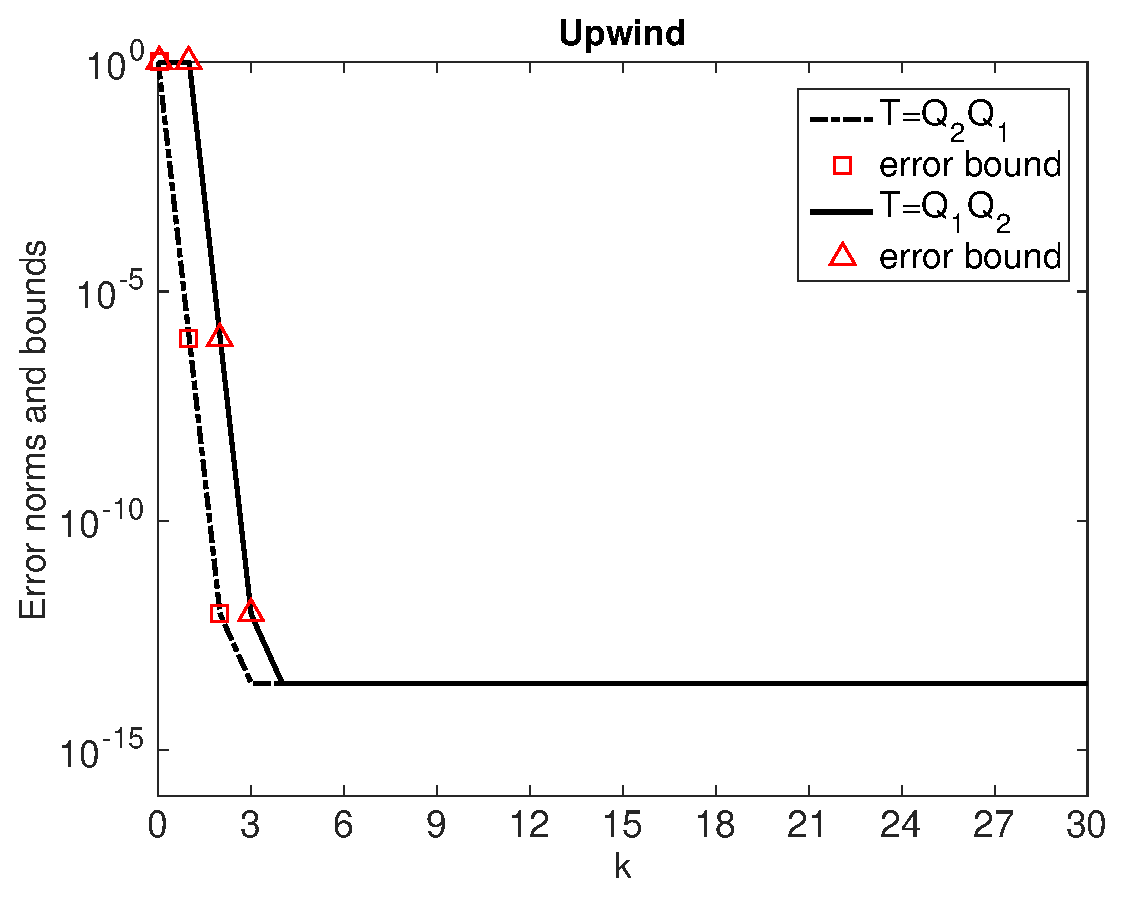
\includegraphics[width=0.95\linewidth]{figures/mSm_upwind_eps_1e-08_N_198}
\end{minipage}
%
\begin{minipage}[t]{0.49\linewidth}
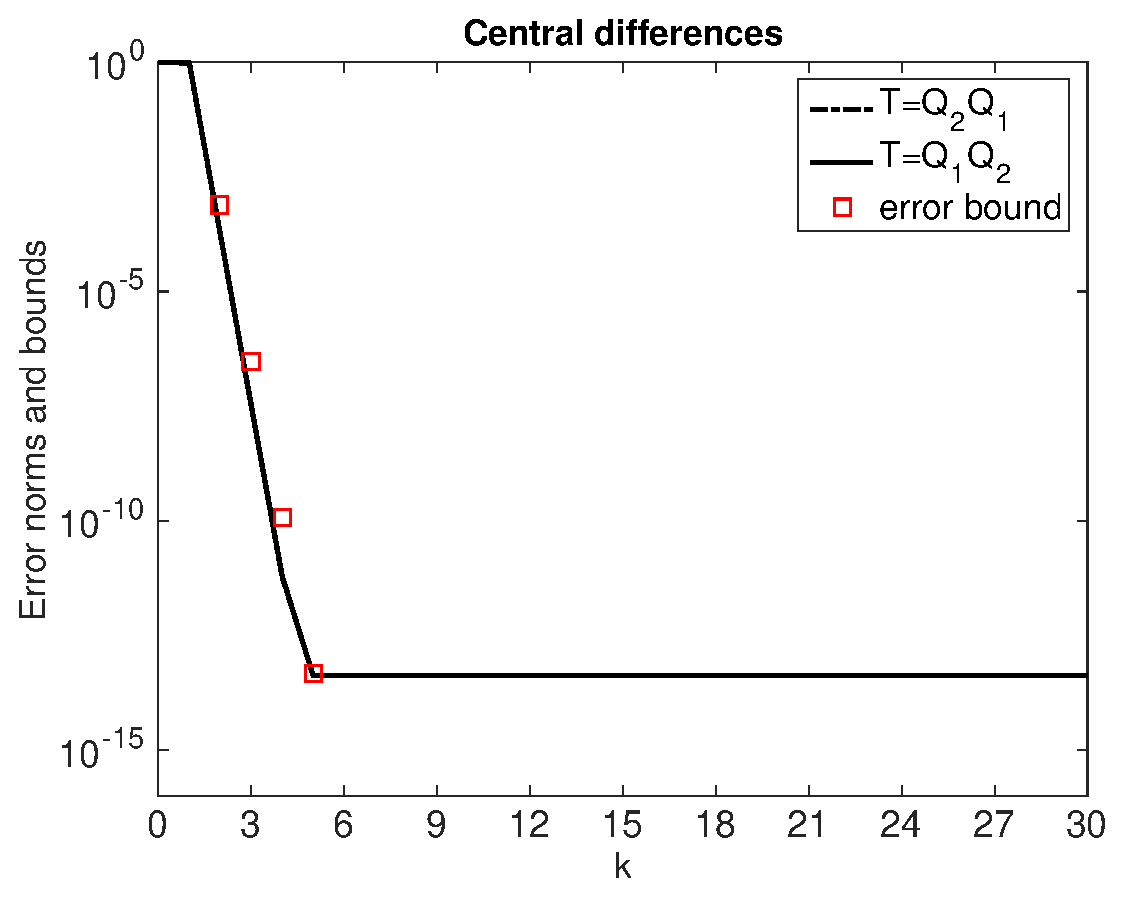
\includegraphics[width=0.95\linewidth]{figures/mSm_central_eps_1e-08_N_198}
\end{minipage}
\caption{Convergence of multiplicative Schwarz and error bounds for
$\epsilon=10^{-8}$, $N=198$, and both discretization schemes.}
%\cblue{Here $|\rho|=9.4\times 10^{-7}<\epsilon(\epsilon+\omega_x H)^{-1}= 9.9 \times 10^{-7}$ for the upwind scheme,
%and $|\rho|=1.8 \times 10^{-4}<2m\epsilon(\epsilon+\omega_x H/2)^{-1}= 3.9 \times 10^{-4}$ for the central differences.}
\label{fig:1D:MSM.N198.eps8}
\end{figure}

\begin{figure}[tbhp]
\begin{minipage}[t]{0.49\linewidth}
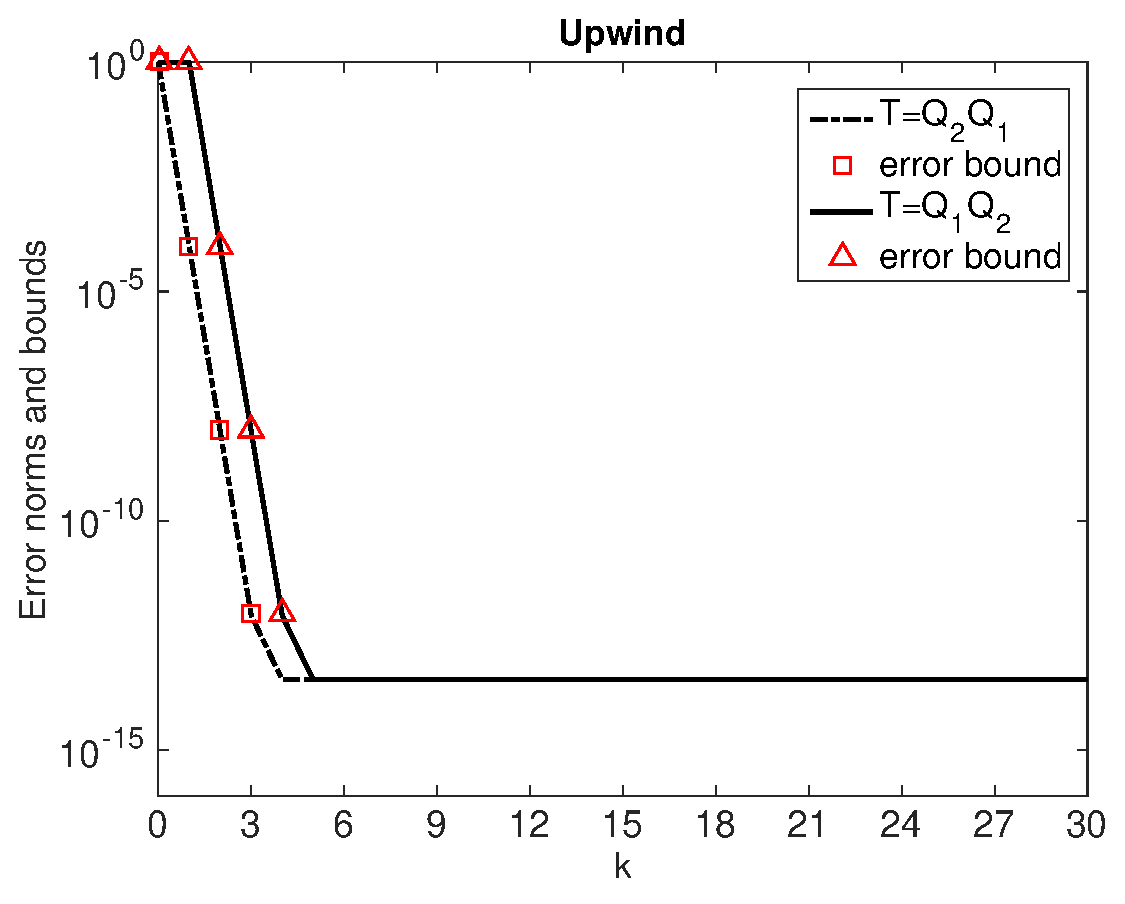
\includegraphics[width=0.95\linewidth]{figures/mSm_upwind_eps_1e-06_N_198}
\end{minipage}
%
\begin{minipage}[t]{0.49\linewidth}
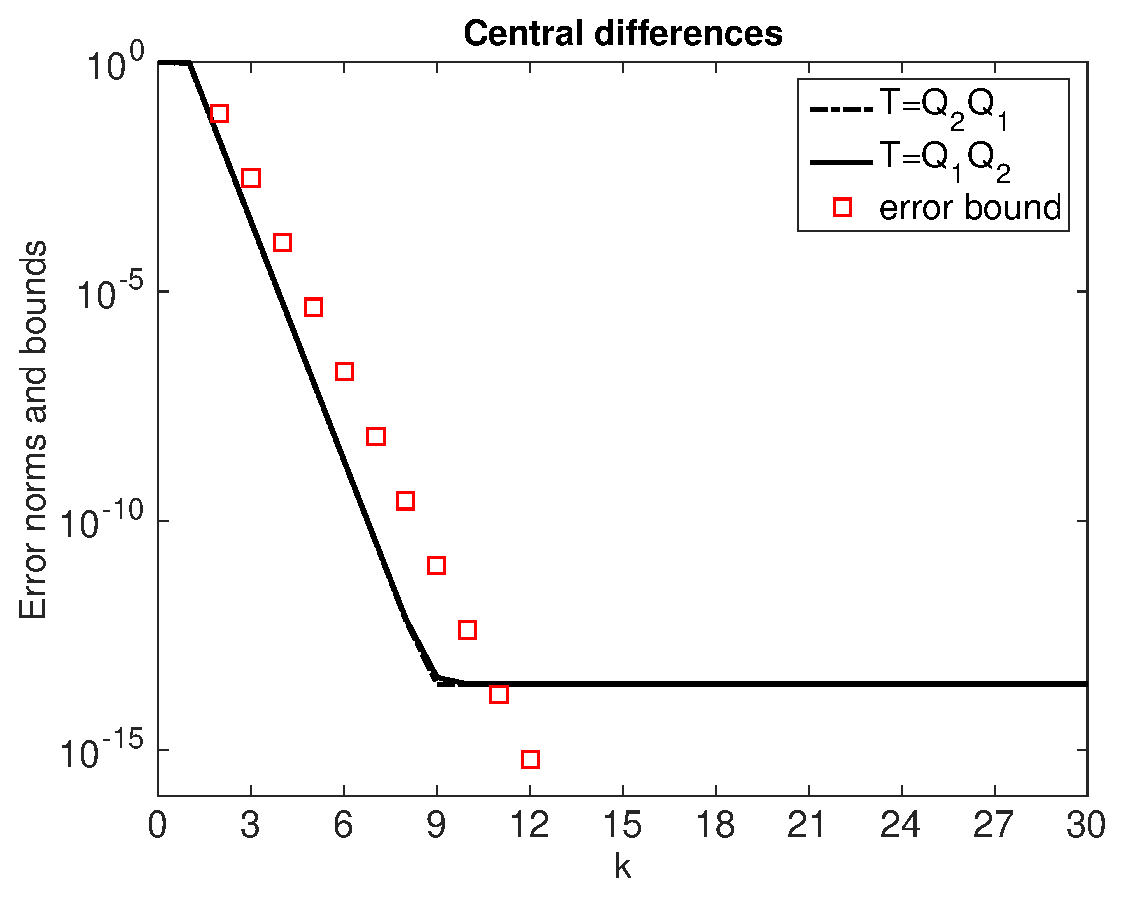
\includegraphics[width=0.95\linewidth]{figures/mSm_central_eps_1e-06_N_198}
\end{minipage}
\caption{Convergence of multiplicative Schwarz and error bounds for
$\epsilon=10^{-6}$, $N=198$, and both discretization schemes.}
%\cblue{Here $|\rho|=9.4\times 10^{-5}<\epsilon(\epsilon+\omega_x H)^{-1}= 9.9 \times 10^{-5}$ for the upwind scheme,
%and $|\rho|=1.8 \times 10^{-2}<2m\epsilon(\epsilon+\omega_x H/2)^{-1}= 3.9 \times 10^{-2}$ for the central differences.}
\label{fig:1D:MSM.N198.eps6}
\end{figure}

\begin{figure}[tbhp]
\begin{minipage}[t]{0.49\linewidth}
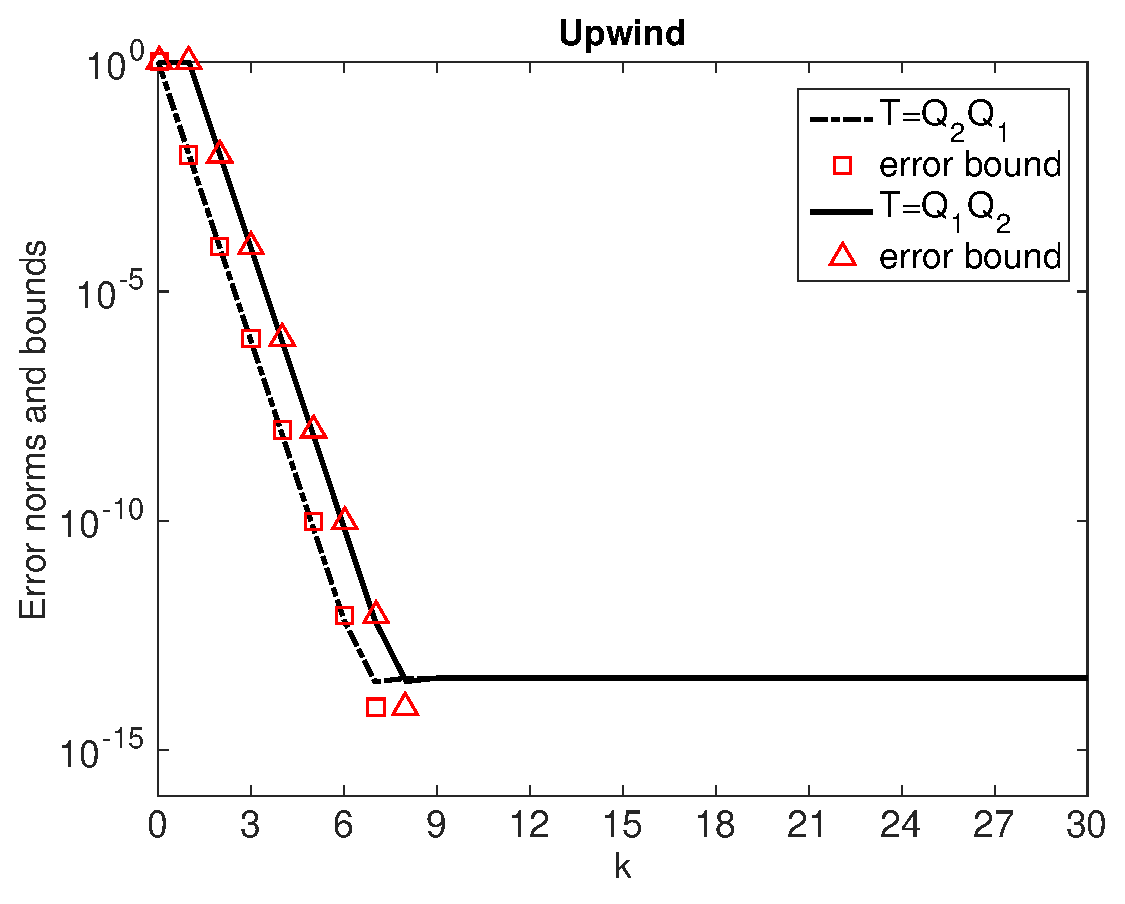
\includegraphics[width=0.95\linewidth]{figures/mSm_upwind_eps_1e-04_N_198}
\end{minipage}
%
\begin{minipage}[t]{0.49\linewidth}
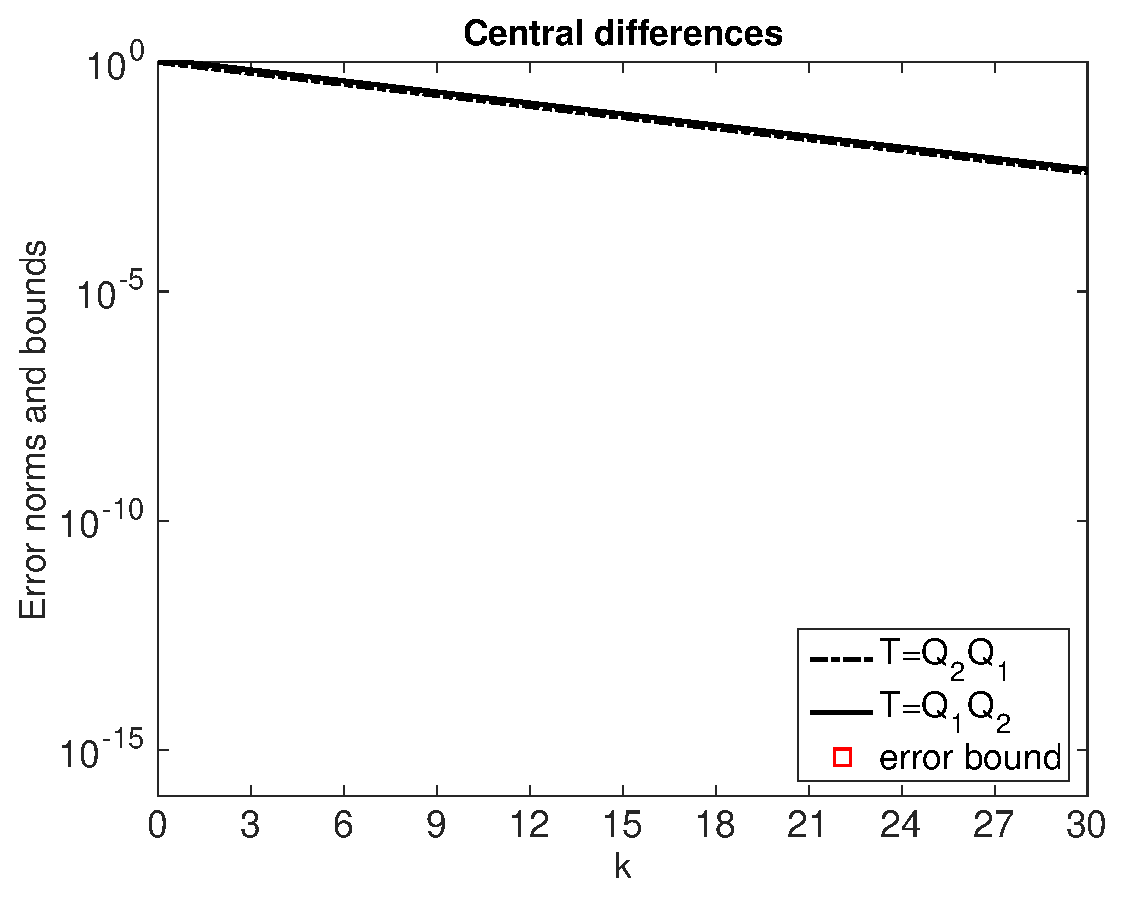
\includegraphics[width=0.95\linewidth]{figures/mSm_central_eps_1e-04_N_198}
\end{minipage}
\caption{Convergence of multiplicative Schwarz and error bounds for
$\epsilon=10^{-4}$, $N=198$, and both discretization schemes.}
%\cblue{Here $|\rho|=9.3\times 10^{-3}<\epsilon(\epsilon+\omega_x H)^{-1}= 9.8 \times 10^{-3}$ for the upwind scheme,
%and $|\rho|=8.3 \times 10^{-1}<2m\epsilon(\epsilon+\omega_x H/2)^{-1}= 3.8$ for the central differences.}
\label{fig:1D:MSM.N198.eps4}
\end{figure}

All numerical results presented in this chapter were performed on a 13-inch
Apple MacBook computer model Mid 2010 with a 2,4 GHz Intel Core 2 Duo
processor. For our experiments we computed $\u=\A^{-1}\f$ using the backslash
operator in \texttt{MATLAB} version R2015b. (Applying iterative refinement in
order to improve the numerical solution obtained in this way yields virtually
the same results, so we do not consider iterative refinement here.) Using the
solution obtained by \texttt{MATLAB}'s backslash, we computed the error norms
of the multiplicative Schwarz method by
$\|\e^{(k)}\|_\infty=\|\u^{(k+1)}-\u\|_\infty$ with $\u^{(k+1)}$
as in \eqref{eq:back:schwarz} and $\u^{(0)}=0$ (rather than using the update
formula $\e^{(k)}=\T_{ij}\e^{(k-1)}$). Consequently, the computed error norms
stagnate on the level of the maximal attainable accuracy of the method.
On the other hand, an error bound of the form $|\rho|^k$ for some
$|\rho|<1$ becomes arbitrarily small for $k\rightarrow\infty$.


\begin{figure}[tbhp]
\begin{minipage}[t]{0.49\linewidth}
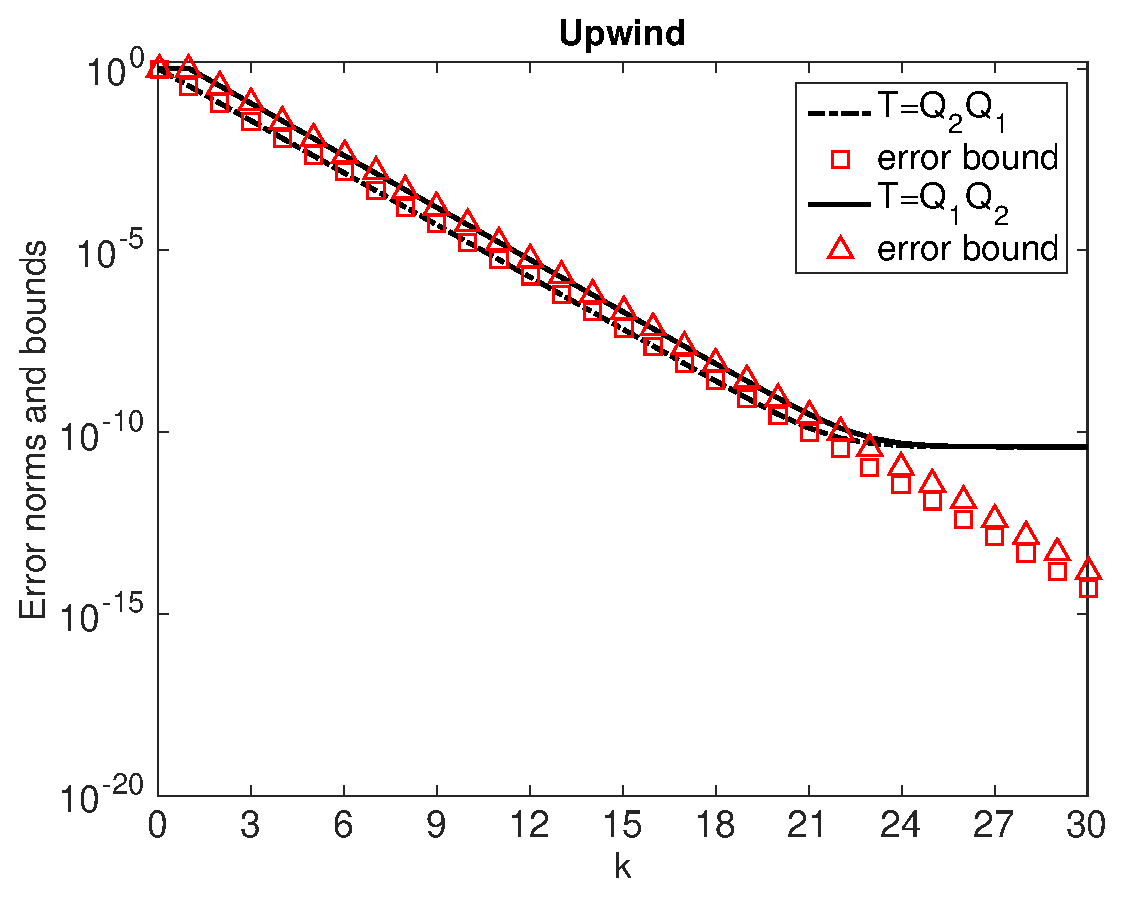
\includegraphics[width=0.95\linewidth]{figures/mSm_upwind_eps_1e-04_N_10002}
\end{minipage}
%
\begin{minipage}[t]{0.49\linewidth}
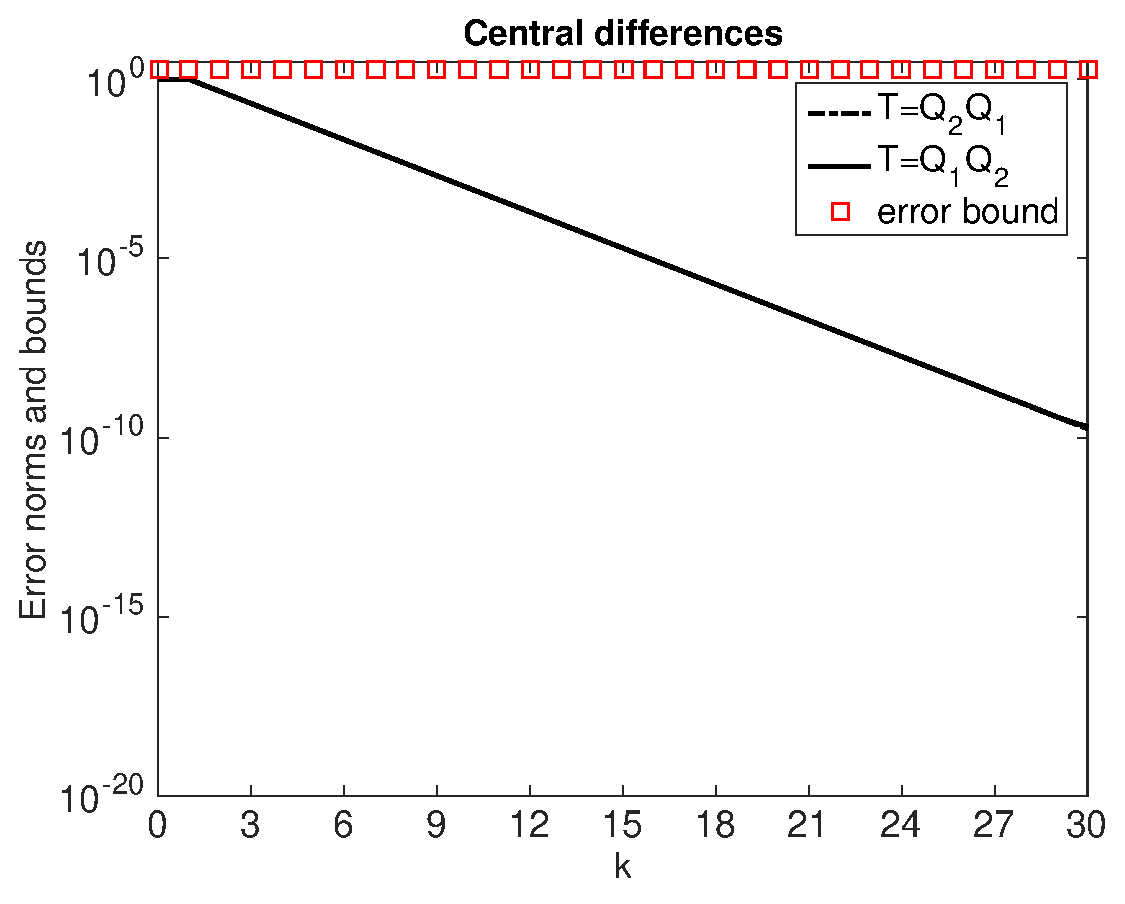
\includegraphics[width=0.95\linewidth]{figures/mSm_central_eps_1e-08_N_10002}
\end{minipage}
\caption{Convergence of multiplicative Schwarz and error bounds for
$\epsilon=10^{-8}$, $N=10002$ and both discretization schemes.}
%\cblue{Here $|\rho|=9.3\times 10^{-3}<\epsilon(\epsilon+\omega_x H)^{-1}= 9.8 \times 10^{-3}$ for the upwind scheme,
%and $|\rho|=8.3 \times 10^{-1}<2m\epsilon(\epsilon+\omega_x H/2)^{-1}= 3.8$ for the central differences.}
\label{fig:1D:MSM.N10002.eps8}
\end{figure}

\begin{figure}[tbhp]
\begin{minipage}[t]{0.49\linewidth}
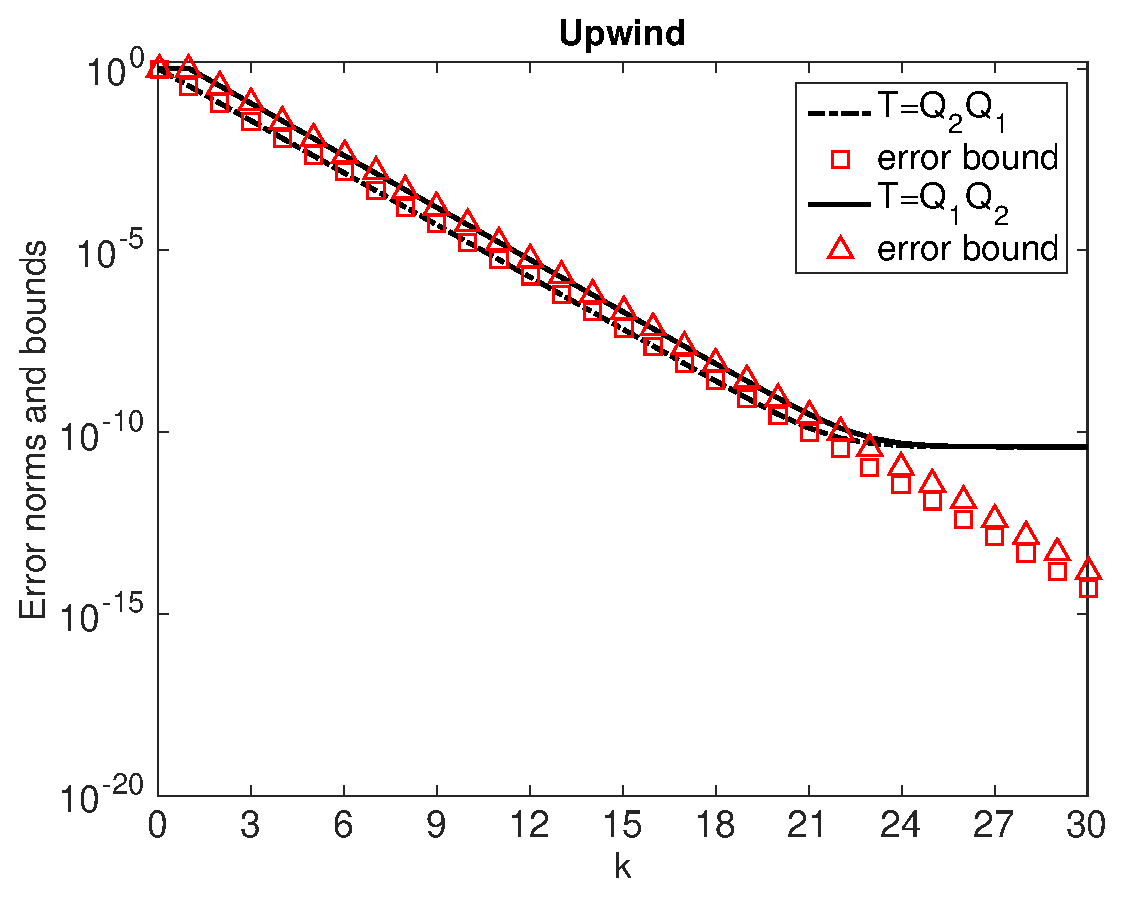
\includegraphics[width=0.95\linewidth]{figures/mSm_upwind_eps_1e-04_N_10002}
\end{minipage}
%
\begin{minipage}[t]{0.49\linewidth}
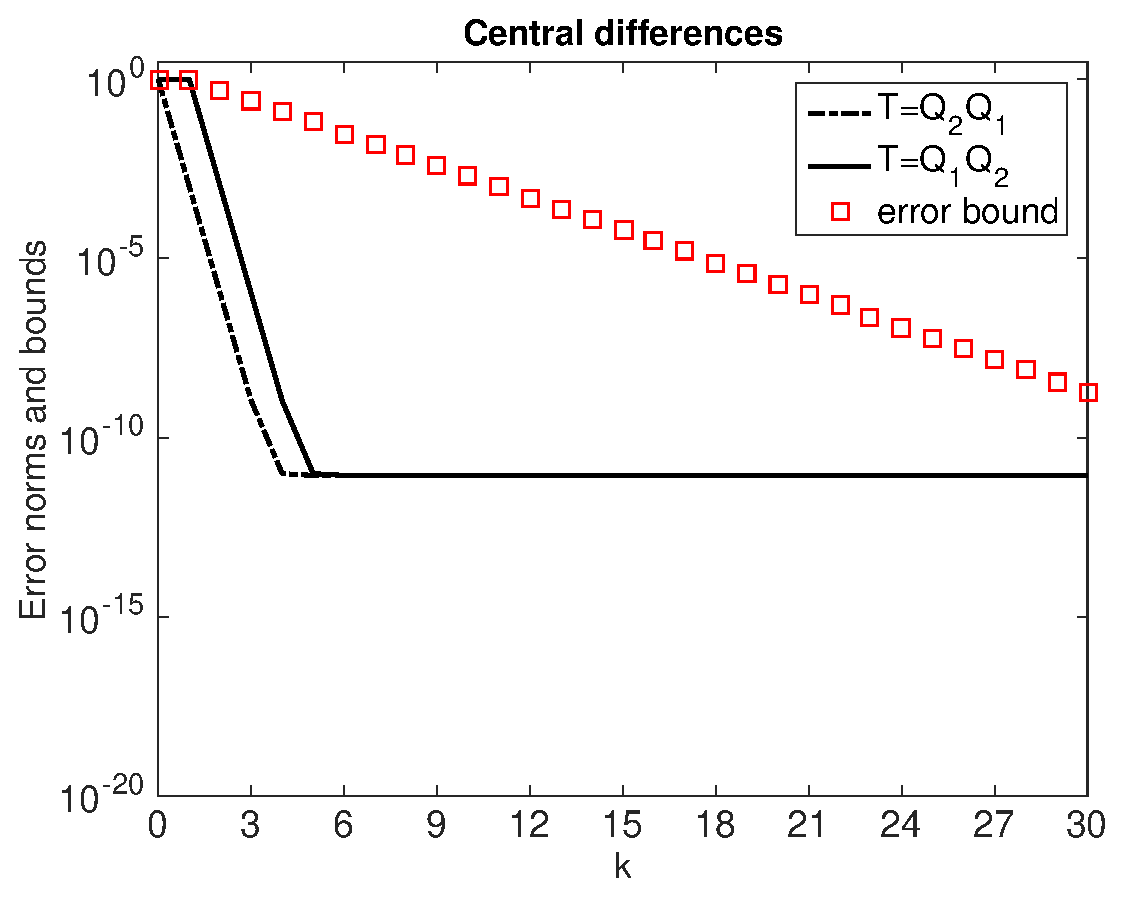
\includegraphics[width=0.95\linewidth]{figures/mSm_central_eps_1e-04_N_10002}
\end{minipage}
\caption{Convergence of multiplicative Schwarz and error bounds for
$\epsilon=10^{-4}$, $N=10002$ and both discretization schemes.}
%\cblue{Here $|\rho|=9.3\times 10^{-3}<\epsilon(\epsilon+\omega_x H)^{-1}= 9.8 \times 10^{-3}$ for the upwind scheme,
%and $|\rho|=8.3 \times 10^{-1}<2m\epsilon(\epsilon+\omega_x H/2)^{-1}= 3.8$ for the central differences.}
\label{fig:1D:MSM.N10002.eps4}
\end{figure}

We start with the upwind discretization. The left parts of
Figures~\ref{fig:1D:MSM.N198.eps8}--\ref{fig:1D:MSM.N10002.eps4}
show the error norms
%
$$\frac{\|\e^{(k)}\|_\infty}{\|\e^{(0)}\|_\infty},\quad  k=0,1,2\dots,$$
%
for the iteration matrices $\T_{12}$ (solid) and $\T_{21}$
(dashed) as well as the corresponding upper bounds from
Theorem~\ref{thm:1D:upwind_conv},
for increasing values of $\epsilon$. We observe that the bounds are
quite close to the actual errors. Moreover, in each case the error norm for
the multiplicative Schwarz method with the iteration matrix $\T_{21}$
almost stagnates in the first step, as predicted by the bound in
Theorem~\ref{thm:1D:upwind_conv}.

On the right parts of Figures~\ref{fig:1D:MSM.N198.eps8}--\ref{fig:1D:MSM.N10002.eps4} we show the
error norms of the multiplicative Schwarz method and the corresponding
convergence bounds from Theorem~\ref{thm:1D:central_conv} for the central
difference scheme.
For our choice of parameters we have $\omega_x H > 2\epsilon$. Note that the
error norms are virtually the same for both iteration matrices. However,
the bounds are not as tight as for the upwind scheme. For fixed $N$ the bounds
become weaker with increasing $\epsilon$, i.e., decreasing convection-
dominance. For our chosen parameters and $\epsilon=10^{-4}$,
giving $\epsilon N^2=\mathscr{O}(1)$, the convergence of the multiplicative
Schwarz method becomes very slow, and the bound~(\ref{eq:1D:bound2}) fails to
predict convergence at all.

We also run the experiments for larger values of $N$. The values of $|\rho|$
and the corresponding bounds from Theorems~\ref{thm:1D:upwind_conv} and
\ref{thm:1D:central_conv} are shown in Table~\ref{tab:1D:rho} for different
values of $N$. We observe that for all cases the bounds on $|\rho|$ for the
upwind scheme are  tighter than for the central difference scheme.
%
\begin{table}[tbhp]
\centering
%\begin{tabular}{rc|c||c|c}
\begin{tabular}{r|c c |c c}
\cline{1-5}
%   & \multicolumn{2}{ c | }{upwind} & \multicolumn{2}{ c }{central differences}\\ \hline
% \multicolumn{1}{ c|   }{$\epsilon$}&$|\rho|$~\eqref{eq:1D:rho} & bound~\eqref{eq:1D:bound_upw} & $|\rho|$~\eqref{eq:1D:rho} & bound~\eqref{eq:1D:bound2}\\
%\hline
\multicolumn{5}{c}{$N=66$}\\\hline
%\multicolumn{1}{ c|  }{$10^{-9}$} & $2.9 \times 10^{-8}$ & $3.3 \times 10^{-8}$ & $1.8 \times 10^{-6}$ & $4.2 \times 10^{-6}$\\
\multicolumn{1}{ c|  }{$10^{-8}$} & $2.9 \times 10^{-7}$ & $3.3 \times 10^{-7}$ & $1.8 \times 10^{-5}$ & $4.2 \times 10^{-5}$\\
\multicolumn{1}{ c|  }{$10^{-6}$} & $2.9 \times 10^{-5}$ & $3.3 \times 10^{-5}$ & $1.8\times 10^{-3}$ & $4.2\times 10^{-3}$\\
\multicolumn{1}{ c|  }{$10^{-4}$} & $2.9 \times 10^{-3}$ & $3.3 \times 10^{-3}$ & $1.8\times 10^{-1}$ & $4.2\times 10^{-1}$\\
\multicolumn{1}{ c|  }{$10^{-2}$} & $2.3 \times 10^{-1}$ & $2.6 \times 10^{-1}$ & $1.3\times 10^{-1}$ & $2.7\times 10^{+1}$\\ \hline
\multicolumn{5}{c}{$N=130$}\\\hline
%\multicolumn{1}{ c|  }{$10^{-9}$} & $6.0 \times 10^{-8}$ & $6.5 \times 10^{-8}$ & $7.7 \times 10^{-6}$ & $1.7 \times 10^{-5}$\\
\multicolumn{1}{ c|  }{$10^{-8}$} & $6.0 \times 10^{-7}$ & $6.5 \times 10^{-7}$ & $7.7 \times 10^{-5}$ & $1.7 \times 10^{-4}$\\
\multicolumn{1}{ c|  }{$10^{-6}$} & $6.0 \times 10^{-5}$ & $6.5 \times 10^{-5}$ & $7.7\times 10^{-3}$ & $1.7\times 10^{-2}$\\
\multicolumn{1}{ c|  }{$10^{-4}$} & $6.0 \times 10^{-3}$ & $6.5 \times 10^{-3}$ & $5.9\times 10^{-1}$ & $1.6\times 10^{~0}$\\
\multicolumn{1}{ c|  }{$10^{-2}$} & $3.8 \times 10^{-1}$ & $4.2 \times 10^{-1}$ & $1.6\times 10^{-1}$ & $5.7\times 10^{-1}$\\ \hline
\multicolumn{5}{c}{$N=258$}\\\hline
%\multicolumn{1}{ c|  }{$10^{-9}$} & $1.2 \times 10^{-7}$ & $1.3 \times 10^{-7}$ & $3.2 \times 10^{-5}$ & $6.6 \times 10^{-5}$\\
\multicolumn{1}{ c|  }{$10^{-8}$} & $1.2 \times 10^{-6}$ & $1.3 \times 10^{-6}$ & $3.2 \times 10^{-4}$ & $6.6 \times 10^{-4}$\\
\multicolumn{1}{ c|  }{$10^{-6}$} & $1.2 \times 10^{-4}$ & $1.3 \times 10^{-4}$ & $3.2\times 10^{-2}$ & $6.6\times 10^{-2}$\\
\multicolumn{1}{ c|  }{$10^{-4}$} & $1.2 \times 10^{-2}$ & $1.3 \times 10^{-2}$ & $8.7\times 10^{-1}$ & $6.4\times 10^{~0}$\\
\multicolumn{1}{ c|  }{$10^{-2}$} & $5.5 \times 10^{-1}$ & $5.9 \times 10^{-1}$ & $4.5\times 10^{-1}$ & $7.2\times 10^{-1}$\\ \hline
\multicolumn{5}{c}{$N=514$}\\\hline
%\multicolumn{1}{ c|  }{$10^{-9}$} & $2.5 \times 10^{-7}$ & $2.6 \times 10^{-7}$ & $1.3 \times 10^{-4}$ & $2.6 \times 10^{-4}$\\
\multicolumn{1}{ c|  }{$10^{-8}$} & $2.5 \times 10^{-6}$ & $2.6 \times 10^{-6}$ & $1.3 \times 10^{-3}$ & $2.6 \times 10^{-3}$\\
\multicolumn{1}{ c|  }{$10^{-6}$} & $2.5 \times 10^{-4}$ & $2.6 \times 10^{-4}$ & $1.3\times 10^{-1}$ & $2.6\times 10^{-1}$\\
\multicolumn{1}{ c|  }{$10^{-4}$} & $2.4 \times 10^{-2}$ & $2.5 \times 10^{-2}$ & $8.6\times 10^{-1}$ & $2.5\times 10^{+1}$\\
\multicolumn{1}{ c|  }{$10^{-2}$} & $7.2 \times 10^{-1}$ & $7.5 \times 10^{-1}$ & $6.8\times 10^{-1}$ & $8.4\times 10^{-1}$\\ \hline
\multicolumn{5}{c}{$N=1026$}\\\hline
%\multicolumn{1}{ c|  }{$10^{-9}$} & $5.1 \times 10^{-7}$ & $5.1 \times 10^{-7}$ & $5.2 \times 10^{-4}$ & $1.1 \times 10^{-3}$\\
\multicolumn{1}{ c|  }{$10^{-8}$} & $5.1 \times 10^{-6}$ & $5.1 \times 10^{-6}$ & $5.2 \times 10^{-3}$ & $1.1 \times 10^{-2}$\\
\multicolumn{1}{ c|  }{$10^{-6}$} & $5.1 \times 10^{-4}$ & $5.1 \times 10^{-4}$ & $4.7\times 10^{-1}$ & $1.0\times 10^{~0}$\\
\multicolumn{1}{ c|  }{$10^{-4}$} & $4.8 \times 10^{-2}$ & $4.9 \times 10^{-2}$ & $7.9\times 10^{-1}$ & $9.5\times 10^{+1}$\\
\multicolumn{1}{ c|  }{$10^{-2}$} & $8.4 \times 10^{-1}$ & $8.6 \times 10^{-1}$ & $8.2\times 10^{-1}$ & $9.1   \times 10^{-1}$\\ \hline
\multicolumn{5}{c}{$N=2050$}\\\hline
%\multicolumn{1}{ c|  }{$10^{-9}$} & $1.0 \times 10^{-6}$ & $1.0 \times 10^{-6}$ & $2.1 \times 10^{-3}$ & $4.2 \times 10^{-3}$\\
\multicolumn{1}{ c|  }{$10^{-8}$} & $1.0 \times 10^{-5}$ & $1.0 \times 10^{-5}$ & $2.1 \times 10^{-2}$ & $4.2 \times 10^{-2}$\\
\multicolumn{1}{ c|  }{$10^{-6}$} & $1.0 \times 10^{-3}$ & $1.0 \times 10^{-3}$ & $9.5\times 10^{-1}$ & $4.2\times 10^{~0}$\\
\multicolumn{1}{ c|  }{$10^{-4}$} & $9.2 \times 10^{-2}$ & $9.3 \times 10^{-2}$ & $6.5\times 10^{-1}$ & $3.5\times 10^{+2}$\\
\multicolumn{1}{ c|  }{$10^{-2}$} & $9.1 \times 10^{-1}$ & $9.2 \times 10^{-1}$ & $9.1\times 10^{-1}$ & $9.5   \times 10^{-1}$\\ \hline
\multicolumn{5}{c}{$N=4098$}\\\hline
%\multicolumn{1}{ c|  }{$10^{-9}$} & $2.0 \times 10^{-6}$ & $2.0 \times 10^{-6}$ & $8.4 \times 10^{-3}$ & $1.7 \times 10^{-2}$\\
\multicolumn{1}{ c|  }{$10^{-8}$} & $2.0 \times 10^{-5}$ & $2.0 \times 10^{-5}$ & $8.3 \times 10^{-2}$ & $1.7 \times 10^{-1}$\\
\multicolumn{1}{ c|  }{$10^{-6}$} & $2.0 \times 10^{-3}$ & $2.0 \times 10^{-3}$ & $9.8\times 10^{-1}$ & $1.7\times 10^{+1}$\\
\multicolumn{1}{ c|  }{$10^{-4}$} & $1.7 \times 10^{-1}$ & $1.7 \times 10^{-1}$ & $4.1\times 10^{-1}$ & $1.2\times 10^{+3}$\\
\multicolumn{1}{ c|  }{$10^{-2}$} & $9.5 \times 10^{-1}$ & $9.6 \times 10^{-1}$ & $9.5\times 10^{-1}$ & $9.8   \times 10^{-1}$\\ \hline
\multicolumn{5}{c}{$N=8194$}\\\hline
\multicolumn{1}{ c|  }{$10^{-8}$} & $4.1 \times 10^{-5}$ & $4.1 \times 10^{-5}$ & $3.2 \times 10^{-1}$ & $6.7 \times 10^{-1}$\\
\multicolumn{1}{ c|  }{$10^{-6}$} & $4.1 \times 10^{-3}$ & $4.1 \times 10^{-3}$ & $9.8 \times 10^{-1}$ & $6.7 \times 10^{+1}$\\
\multicolumn{1}{ c|  }{$10^{-4}$} & $2.9 \times 10^{-1}$ & $2.9 \times 10^{-1}$ & $9.8 \times 10^{-2}$ & $3.7 \times 10^{+3}$\\
\multicolumn{1}{ c|  }{$10^{-2}$} & $9.8 \times 10^{-1}$ & $9.8 \times 10^{-1}$ & $9.8 \times 10^{-1}$ & $9.9 \times 10^{-1}$\\
% & \multicolumn{2}{ c | }{upwind} & \multicolumn{2}{ c }{central differences}\\
%\hline
\multicolumn{1}{ c|   }{$\epsilon$}&$|\rho|$~\eqref{eq:1D:rho} & bound~\eqref{eq:1D:bound_upw} & $|\rho|$~\eqref{eq:1D:rho} & bound~\eqref{eq:1D:bound2}\\ \hline
& \multicolumn{2}{ c | }{upwind} & \multicolumn{2}{ c }{central differences}\\
\hline
\end{tabular}
\caption{Values of $|\rho|$ computed using \eqref{eq:1D:rho} and the corresponding bounds (\ref{eq:1D:bound_upw}) and (\ref{eq:1D:bound2}) for different values of $\epsilon$ and $N$.}
\label{tab:1D:rho}
\end{table}

To further illustrate our results, we also present the results for a larger
value of $N$, namely $N=10002$. We consider the special cases
$\epsilon N^2 \approx 1$ (Figure~\ref{fig:1D:MSM.N10002.eps8})
and $\epsilon N \approx 1$ (Figure~\ref{fig:1D:MSM.N10002.eps4})
which are mainly of theoretical interest. While the bound
\eqref{eq:1D:bound_upw} for the upwind scheme is still tight and descriptive,
the bound~\eqref{eq:1D:bound2} for the central difference scheme does not
predict convergence well. Note that the parameters used in
Figure~\ref{fig:1D:MSM.N10002.eps4} yield
$\omega_x H\approx 1.9959\times 10^{-4} < 2\epsilon$, and hence the right part
of Figure~\ref{fig:1D:MSM.N10002.eps4} shows error norms and the convergence
bound corresponding to the case $\omega_x H\leq 2\epsilon$ in
Theorem~\ref{thm:1D:central_conv}.

We continue our numerical experiments by applying GMRES to the linear
algebraic system \emph{preconditioned with multiplicative Schwarz}, i.e., the
linear algebraic system \eqref{eq:1D:precond}, in the case $N=198$. Using the
2-norm, the (preconditioned) relative residual norms are shown in
Figures~\ref{fig:1D:GMRES.N198.eps6.prec}--\ref{fig:1D:GMRES.N198.eps8.prec}
and were computed using \texttt{MATLAB}'s command \texttt{gmres} with a
tolerance of $10^{-14}$, a maximum number of iterations of $N-1$ and initial
approximation $\u^{(0)}=0$. In all cases convergence is achieved in two
iterations, which is explained in the previous section. These figures are the
counterparts to
Figures~\ref{fig:back:GMRES.N198.eps4}--\ref{fig:back:GMRES.N198.eps8},
where GMRES makes little progress until iteration 198.

\begin{figure}[tbhp]
\begin{minipage}[t]{0.48\linewidth}
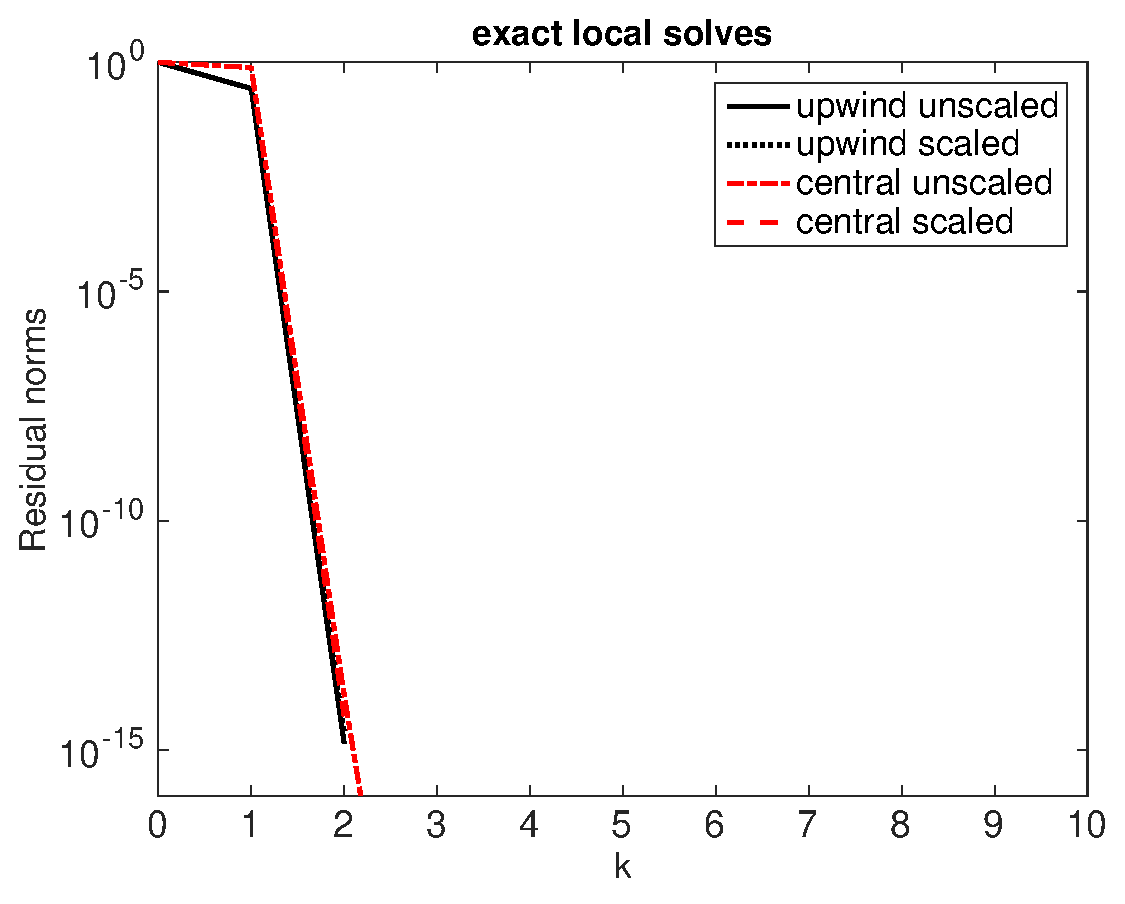
\includegraphics[width=0.98\linewidth]{figures/gmres_eps_1e-02_N_198_prec}
%\label{fig:1D:GMRES.N198.eps4.prec}
% note: if changing to 3 figures again, it needs to be changed in two places
%\caption{Preconditioned GMRES convergence for $\epsilon=10^{-4}$.}
\end{minipage}
%
\begin{minipage}[t]{0.48\linewidth}
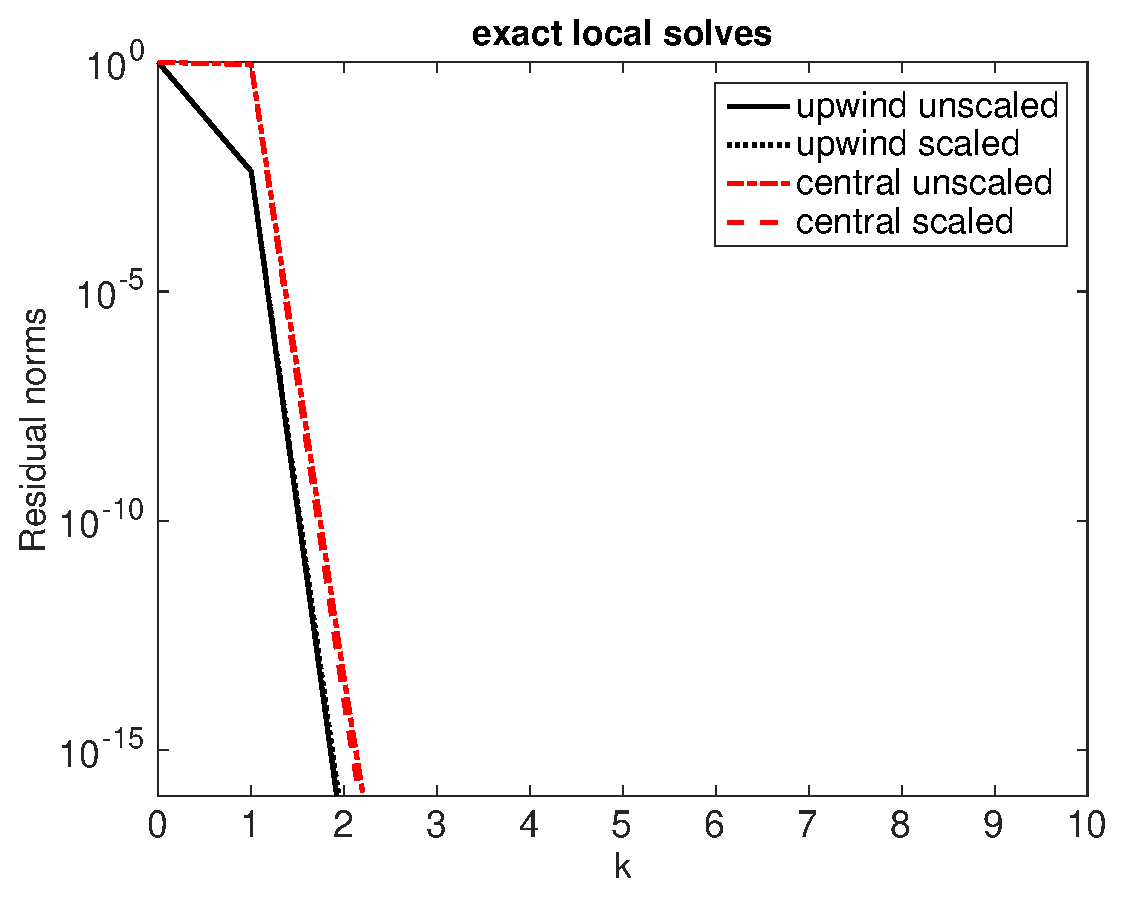
\includegraphics[width=0.98\linewidth]{figures/gmres_eps_1e-04_N_198_prec}
\end{minipage}
\caption{Preconditioned GMRES convergence for $\epsilon=10^{-2}$ [l.] and $\epsilon=10^{-4}$ [r.]}
\label{fig:1D:GMRES.N198.eps6.prec}
\end{figure}
%
\begin{figure}[tbhp]
\begin{minipage}[t]{0.48\linewidth}
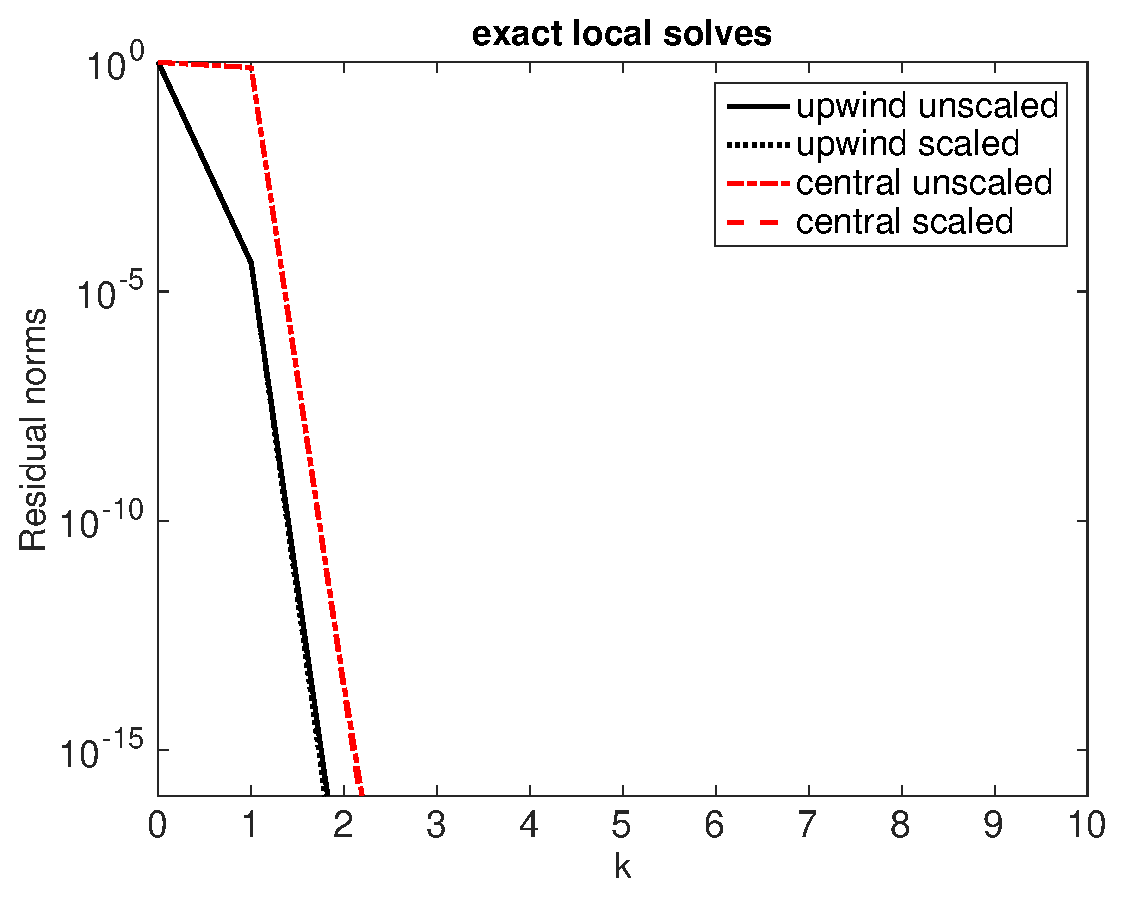
\includegraphics[width=0.98\linewidth]{figures/gmres_eps_1e-06_N_198_prec}
%\label{fig:1D:GMRES.N198.eps4.prec}
% note: if changing to 3 figures again, it needs to be changed in two places
%\caption{Preconditioned GMRES convergence for $\epsilon=10^{-4}$.}
\end{minipage}
%
\begin{minipage}[t]{0.48\linewidth}
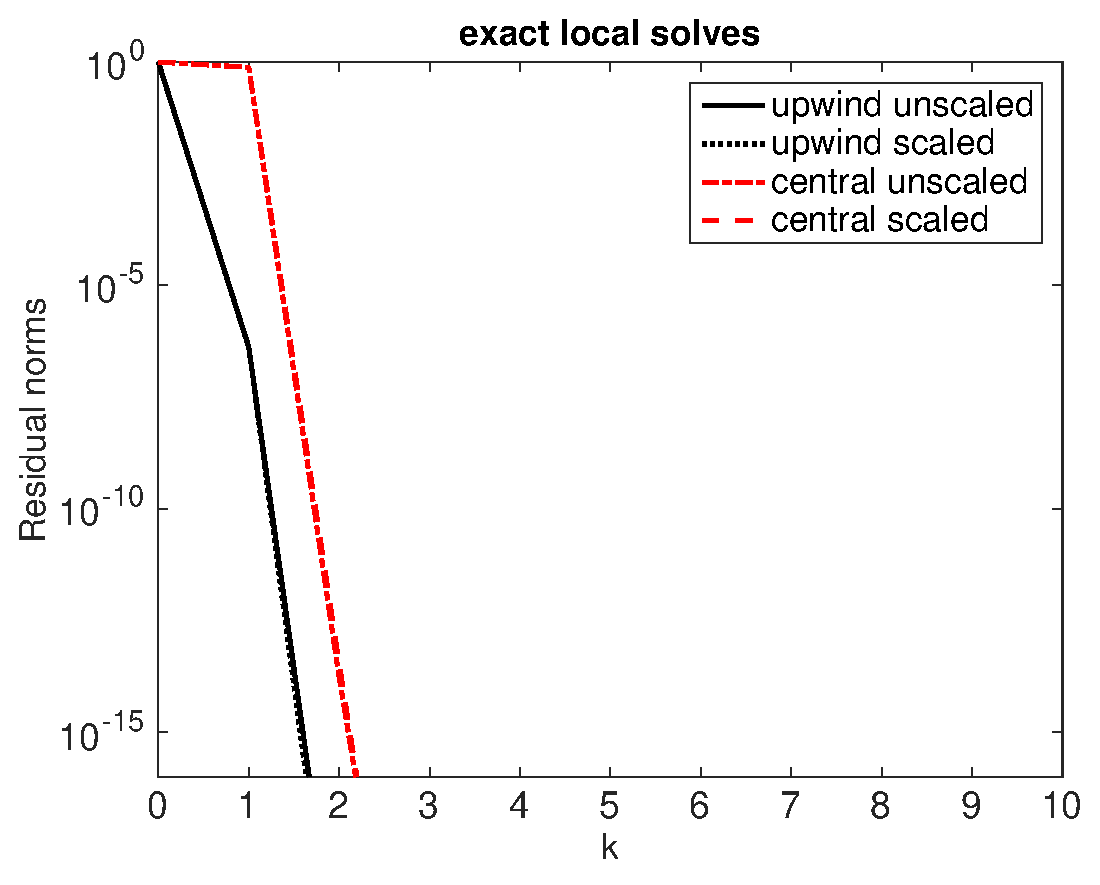
\includegraphics[width=0.98\linewidth]{figures/gmres_eps_1e-08_N_198_prec}
\end{minipage}
\caption{Preconditioned GMRES convergence for $\epsilon=10^{-6}$ [l.] and $\epsilon=10^{-8}$ [r.].}
\label{fig:1D:GMRES.N198.eps8.prec}
\end{figure}
%
% \begin{figure}[h!]
% \hspace{-1cm}
% \centering
% \begin{minipage}[t]{0.78\linewidth}
% \centering
% 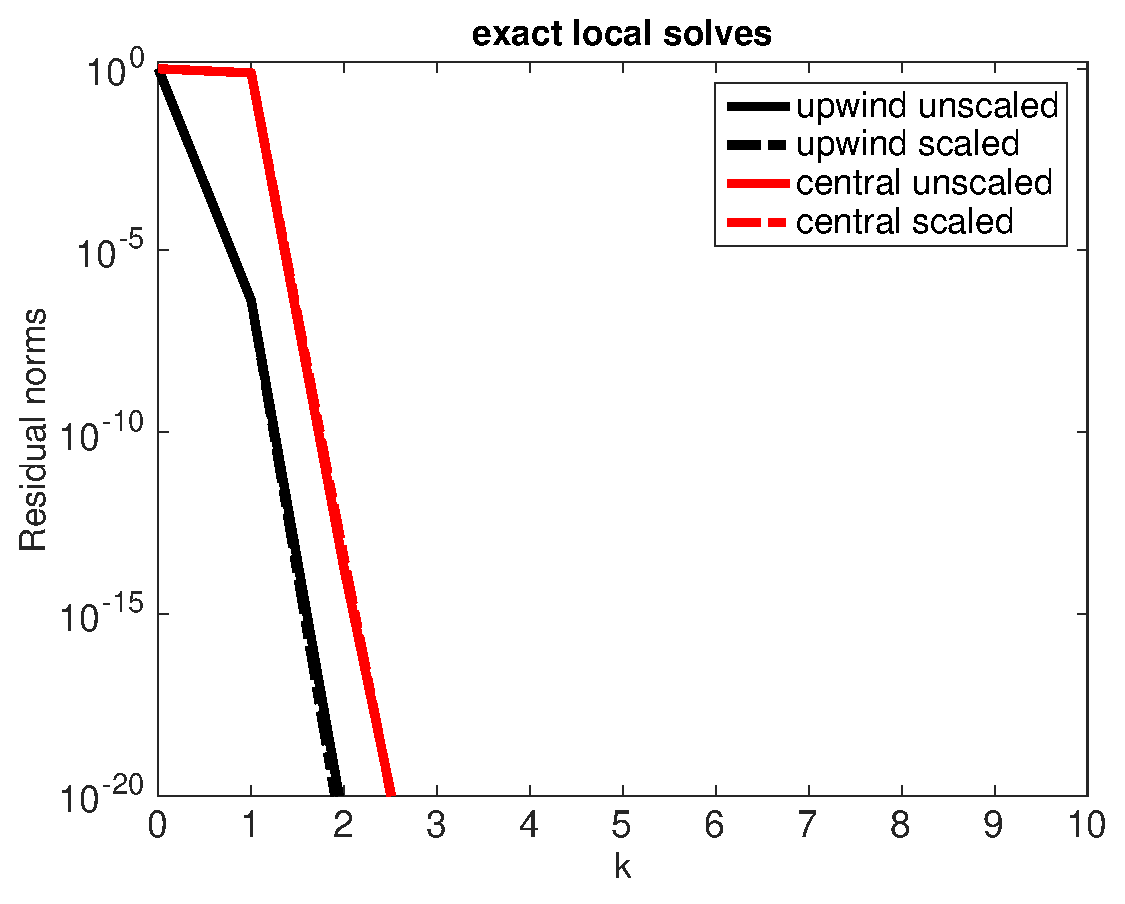
\includegraphics[width=0.6\linewidth]{figures/gmres_8_198_prec}
% \caption{Preconditioned GMRES convergence for $\epsilon~=~10^{-8}$.}
% \label{fig:1D:GMRES.N198.eps8.prec}
% \end{minipage}
% \end{figure}

% \begin{figure}[tbhp]
% \begin{minipage}[t]{0.48\linewidth}
% 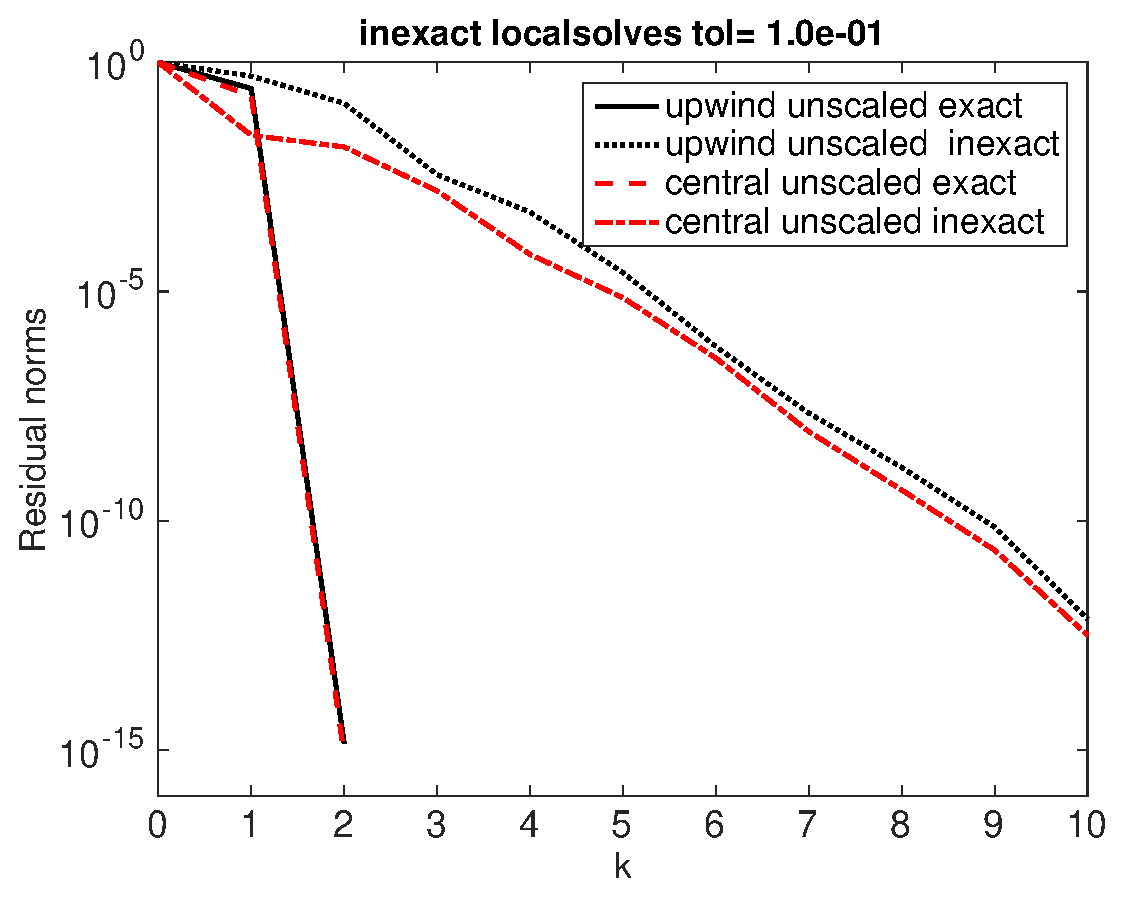
\includegraphics[width=0.98\linewidth]{figures/gmres_8_198_inexact-1e-01}
% %\label{fig:1D:GMRES.N198.eps4.prec}
% % note: if changing to 3 figures again, it needs to be changed in two places
% %\caption{Preconditioned GMRES convergence for $\epsilon=10^{-4}$.}
% \end{minipage}
% %
% \begin{minipage}[t]{0.48\linewidth}
% 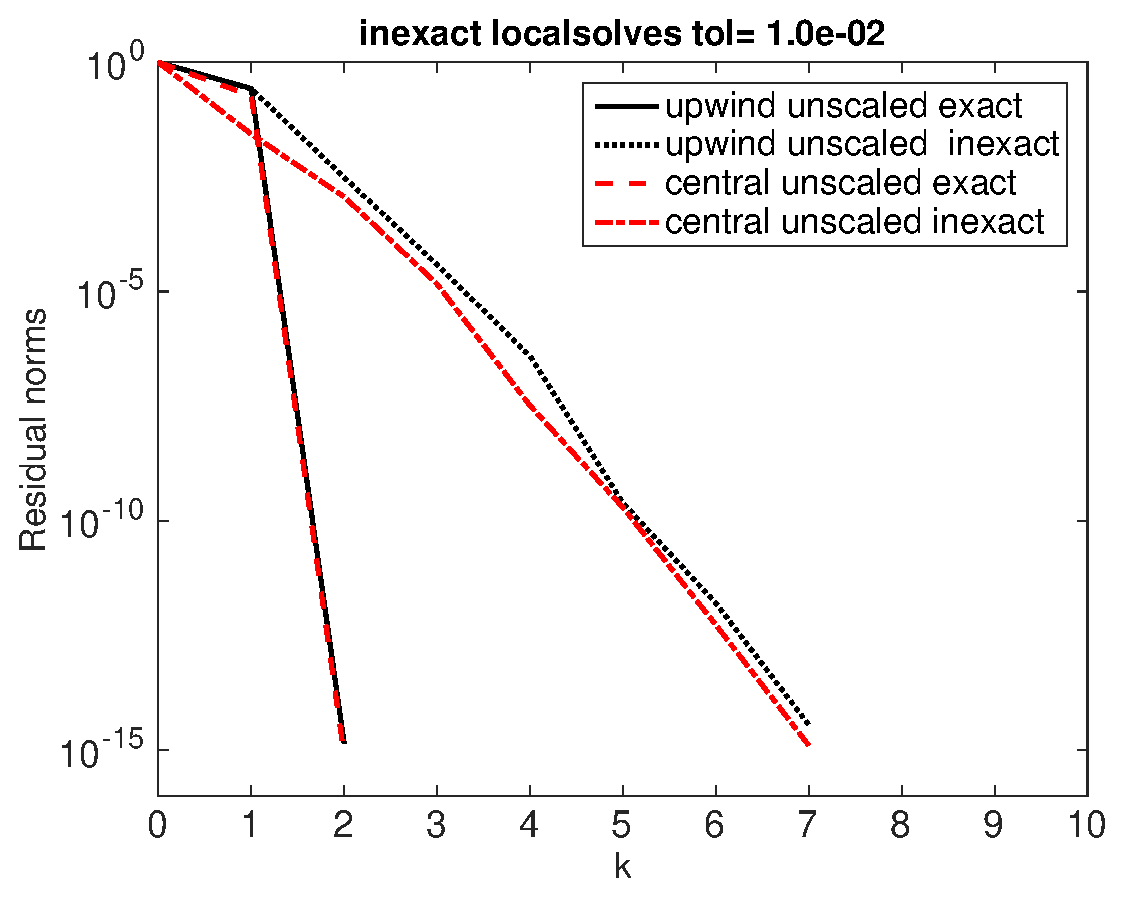
\includegraphics[width=0.98\linewidth]{figures/gmres_8_198_inexact-1e-02}
% \end{minipage}
% \caption{Preconditioned GMRES convergence for $\epsilon~=~10^{-8}$ [l.] with inexact local solve tolerance of $10^{-1}$ and $10^{-2}$ [r.].}
% \label{fig:1D:GMRES.inexact.prec.N198.eps8.tol1_2}
% \end{figure}
% %
% \begin{figure}[tbhp]
% \hspace{-1cm}
% \centering
% \begin{minipage}[t]{0.48\linewidth}
% \centering
% 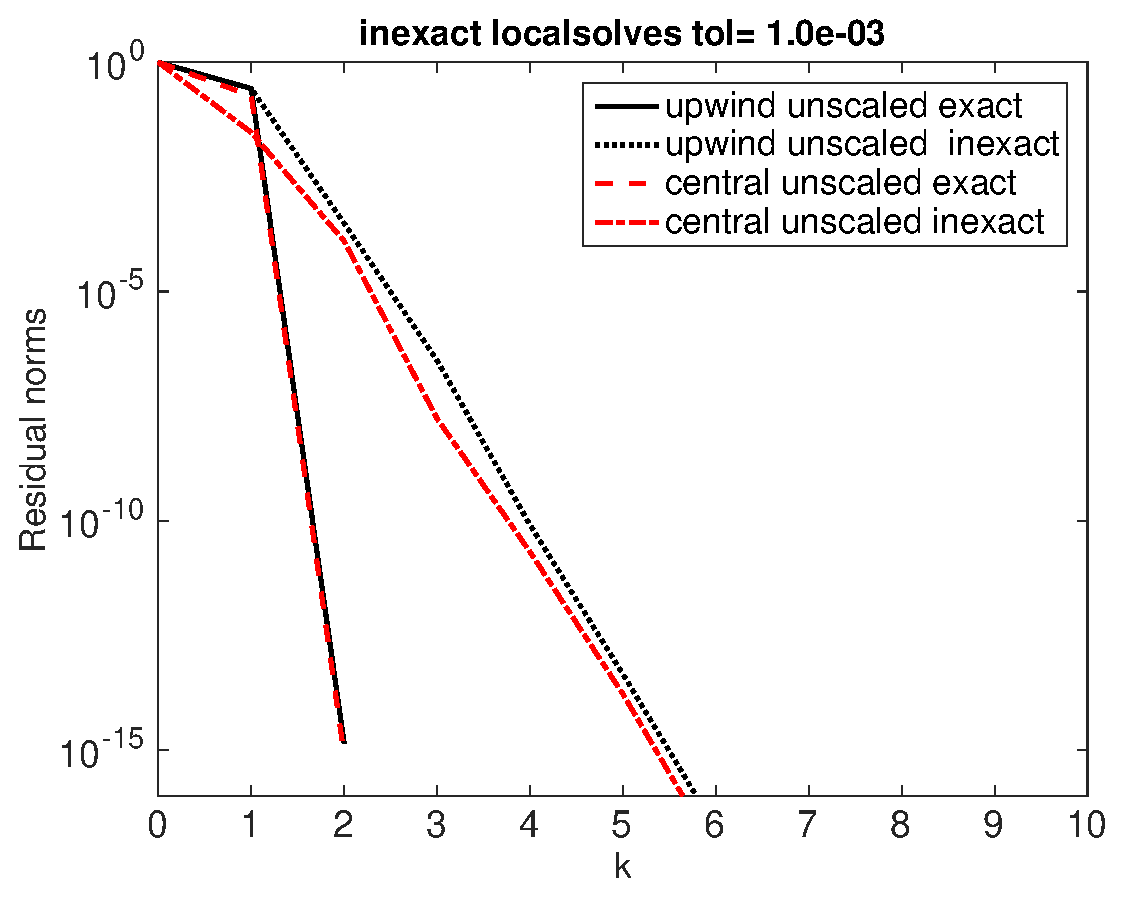
\includegraphics[width=0.98\linewidth]{figures/gmres_8_198_inexact-1e-03}
% \end{minipage}
% %
% \begin{minipage}[t]{0.48\linewidth}
% 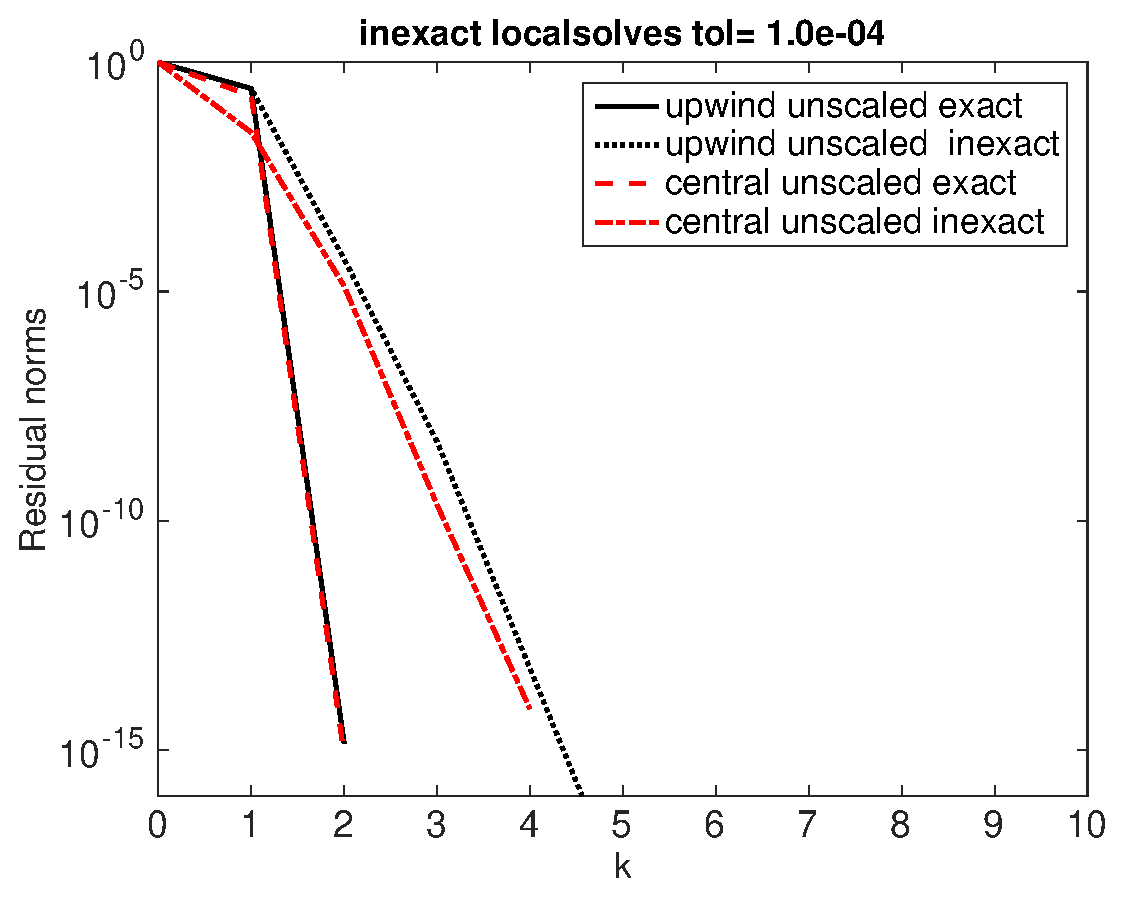
\includegraphics[width=0.98\linewidth]{figures/gmres_8_198_inexact-1e-04}
% \end{minipage}
% \caption{Preconditioned GMRES convergence for $\epsilon~=~10^{-8}$ with inexact local solve tolerance of $10^{-3}$ [l.] and $10^{-4}$ [r.].}
% \label{fig:1D:GMRES.inexact.prec.N198.eps8.tol3_4}
% \end{figure}
%
% We conclude our numerical experiments by presenting results for the
% preconditioned GMRES method for the case of when the local subdomain problems
% are solved inexactly. Figures~\ref{fig:1D:GMRES.inexact.prec.N198.eps8.tol1_2}--\ref{fig:1D:GMRES.inexact.prec.N198.eps8.tol3_4} again show the
% preconditioned relative residual norms for the case where the local subdomain
% problems are solved inexactly using the GMRES method for the case of $N=198$
% and $\epsilon=10^{-8}$.
% %(See right side of Figure\ref{fig:1D:GMRES.N198.eps8.prec}).
% For this value of the perturbation parameter, the figures show that choosing a
% tolerance of $10^{-2}$ for the relative residual norm in the solution of
% the local subdomain problems, the number of steps needed for the convergence
% of GMRES to reach a normwise relative residual norm of $10^{-14}$ in the
% global system (outer iteration) for the upwind scheme grows from 2 to 4 steps
% and for the central difference scheme it grows form 2 to 5 steps only. With a
% local tolerance of $10^{-4}$ both the upwind as well as the central difference
% schemes converge in 3 iterations to reach the same relative residual norm in
% the outer iteration as solving the local subdomain problems exactly.
%
% Table~\ref{tab:1D:GMRES.inexact.prec} %--\ref{tab:1D:inexact_central}
% shows the number of iterations needed for the outer iteration to achieve the
% same relative residual norm for different values of $\epsilon$. As
% expected, the inexact methods exhibit slower convergence and do not converge
% in $r+1$ steps, where $r$ is the rank of the iteration matrix $\T_{ij}$ (we
% have shown that $r=1$ in the case of the 1D model problem, see
% \eqref{eq:1D:struct1} and \eqref{eq:1D:struct2}). Nevertheless, they converge
% in less computational time if the saving from the inexact local solve is
% sufficiently large to offset the loss in convergence steps. This is often the
% case in practice as noted by Benzi, Frommer, Nabben and Szyld
% in~\cite[\S~4]{BenFroNabSzy01}.
% %
%
% \begin{table}[tbph]
% \centering
% \vspace*{-0.2em}
% \begin{tabular}{r|cccccc}
% %\cline{1-5}
% \hline
% \multicolumn{7}{c}{upwind scheme}\\\hline
% \multicolumn{1}{c|}{\diagbox{$\epsilon$}{tol}} & $10^{-1}$ & $10^{-2}$ & $10^{-3}$ & $10^{-4}$ & $10^{-5}$ & $10^{-6}$\\
% \hline
% \multicolumn{1}{c|}{$10^{-8}$} & $12$ & $5$ & $4$ & $4$ & $4$ & $4$\\
% \multicolumn{1}{c|}{$10^{-6}$} & $12$ & $6$ & $5$ & $4$ & $3$ & $3$\\
% \multicolumn{1}{c|}{$10^{-4}$} & $12$ & $7$ & $4$ & $4$ & $3$ & $3$\\
% \multicolumn{1}{c|}{$10^{-2}$} & $12$ & $7$ & $6$ & $5$ & $4$ & $4$\\
% \hline
% \multicolumn{7}{c}{central differences scheme}\\\hline
% \multicolumn{1}{c|}{\diagbox{$\epsilon$}{tol}} & $10^{-1}$ & $10^{-2}$ & $10^{-3}$ & $10^{-4}$ & $10^{-5}$ & $10^{-6}$\\
% \hline
% \multicolumn{1}{c|}{$10^{-8}$} & $13$ & $6$ & $5$ & $4$ & $3$ & $2$\\
% \multicolumn{1}{c|}{$10^{-6}$} & $13$ & $6$ & $5$ & $4$ & $3$ & $2$\\
% \multicolumn{1}{c|}{$10^{-4}$} & $15$ & $7$ & $5$ & $4$ & $3$ & $2$\\
% \multicolumn{1}{c|}{$10^{-2}$} & $12$ & $7$ & $6$ & $4$ & $4$ & $4$\\
% \end{tabular}
% \caption{Iteration count for GMRES with inexact Shishkin-Schwarz preconditioning to reach a relative residual norm of $10^{-14}$ for problem~\eqref{eq:1D:bvp} with $N=198$ and different local solve tolerances.}
% \label{tab:1D:GMRES.inexact.prec}
% \end{table}

%
% \begin{table}
% \centering
% \begin{tabular}{r|cccccc}
% %\cline{1-5}
% \hline
% \multicolumn{7}{c}{central differences scheme}\\\hline
% \multicolumn{1}{c|}{\diagbox{$\epsilon$}{tol}} & $10^{-1}$ & $10^{-2}$ & $10^{-3}$ & $10^{-4}$ & $10^{-5}$ & $10^{-6}$\\
% \hline
% \multicolumn{1}{c|}{$10^{-8}$} & $13$ & $6$ & $5$ & $4$ & $3$ & $2$\\
% \multicolumn{1}{c|}{$10^{-6}$} & $13$ & $6$ & $5$ & $4$ & $3$ & $2$\\
% \multicolumn{1}{c|}{$10^{-4}$} & $15$ & $7$ & $5$ & $4$ & $3$ & $2$\\
% \multicolumn{1}{c|}{$10^{-2}$} & $12$ & $7$ & $6$ & $4$ & $4$ & $4$\\
% \end{tabular}
% \caption{Iteration count for GMRES with inexact Shishkin-Schwarz preconditioning to reach a relative  residual norm of $10^{-14}$ for the 1D model problem with $N=198$ and different local tolerances using the central difference scheme.}
% \label{tab:1D:inexact_central}
% \end{table}
%
%
% \subsection{Upwind Finite Differences}
%
% \begin{figure}[h!]
% \centering
% \missingfigure[figwidth=10cm]{Numerical experiments for upwind finite differences}
% \caption{GMRES convergence for...}
% \label{fig:1D:GMRES.upwind}
% \end{figure}
%
% \subsection{Central Finite Differences}
%
% \begin{figure}[h!]
% \centering
% \missingfigure[figwidth=10cm]{Numerical experiments for central finite differences}
% \caption{GMRES convergence for...}
% \label{fig:1D:GMRES.central}
% \end{figure}

%\cred{Finally, we conclude our numerical experiments with an example
%\cblue{for the central differences scheme, showing the behavior of the considered linear solvers in the case %when $m=N/2-1$ is odd. Recall that if $m$ is odd, we are not able to bound the terms which appear in
%the explicit form of $\rho$ (see \eqref{eq:1D:rho}) as in Lemma~\ref{lem:p4}.
%In the experiment we choose $\epsilon=10^{-3}$ and $N=20$ so that $m=9$.
%In the right part of Figure~\ref{fig6} we see that the multiplicative Schwarz method diverges and obviously %$|\rho|>1$. In the right part
%of Figure~\ref{fig6} we apply GMRES to the system preconditioned
%with multiplicative Schwarz.
%
%\begin{figure}
%\begin{minipage}[t]{0.48\linewidth}
%\includegraphics[width=0.98\linewidth]{figures/central_3_20}
%\end{minipage}
%
%\begin{minipage}[t]{0.48\linewidth}
%\includegraphics[width=0.98\linewidth]{figures/gmres_3_20_prec}
%\end{minipage}
%\cblue{\caption{Convergence history of multiplicative Schwarz (left) and GMRES (right) for $\epsilon=10^{-3}$, %$N=20$.}\label{fig6}}
%\end{figure}
%
%As in the case of an even $m$, convergence of GMRES is achieved
%in two iterations. This is not surprising thanks to the low rank structure of the iteration matrix, as we will %explain in detail in the  next section. To check the quality of the solution obtained by the preconditioned %GMRES method we computed the relative distance
%$$
%	\frac{\| \bar{x}-x_2\|}{\|\bar{•}{x}\|},
%$$
%where $x_2$ is the GMRES solution and $\bar{x}$ is the solution computed by  \texttt{MATLAB}'s backslash operator. %The resulting relative distance is about $???$, and $\|\bar{x}\| \approx ???$.
% }}



%\begin{figure}
%\begin{minipage}[t]{0.48\linewidth}
%\includegraphics[width=0.98\linewidth]{figures/solutions_1_20}
%%\caption{Convergence of multiplicative Schwarz and error bounds for $\epsilon=10^{-3}$, $N=20$.}
%\end{minipage}
%%
%\begin{minipage}[t]{0.48\linewidth}
%\includegraphics[width=0.98\linewidth]{figures/solutions_2_20}
%%\caption{GMRES convergence for $\epsilon=10^{-3}$.}\label{fig9}
%\end{minipage}
%\cred{\caption{Solution of \eqref{eq:bvp} with $\epsilon=10^{-3}$, $\omega_x=1$, $\beta=0$, $f(x)\equiv 1$, $u_0=u_1=0$, and, $N=20$. }\label{fig8}}
%\end{figure}

%As we can see, even though the multiplicative Schwarz method does not converge in this case providing an unsatisfactory numerical solution, the preconditioned system is solved to a desired accuracy yielding and acceptable numerical solution to the problem. Thus we have shown that the restriction of choosing an even number of points in the local subdomains does not affect the performance of the method used as a preconditioner. We provide the following explanation; since
%$$
%\rho(T)\leq\|T\|\leq\gamma<1,
%$$
%the preconditioned system $M^{-1}A=T=I-M^{-1}N$ will have eigenvalues
%$$
%\lambda(M^{-1}A)\subseteq \left\{ z\in\mathbb{R}: |z|<1+\gamma\right\}.
%$$
%We can therefore expect that the GMRES method converges independently of the number of discretization points used in the method as long as the norm of the iteration matrix is less than one.



\fi % end of if statement regarding content shown


%\addtocontents{toc}{\protect\newpage}%forces pagebreak in ToC
\chapter{The Theory of Block Diagonal Dominant Matrices}
\label{ch:BDiDo}
\ifnum\switch=1
% -----------------------------------------------------------------------------
% ------------------------------ Extended ToC ---------------------------------
% -----------------------------------------------------------------------------

Parts of this chapter have already been published in:
\begin{enumerate}
\item[\cite{EchLieNab18}] \underline{C.~Echeverr{\'\i}a}, J.~Liesen, and R.~Nabben, \textbf{Block diagonal dominace of matrices revisited: Bounds for the norms of inverses and eigenvalue inclusion sets}, Linear Algebra Appl., 553 (2018), pp. 365--383.
\end{enumerate}


\section{Introduction}
This section is based on the following references: \cite{BerPle94, FonPet01, Ike79, Nabben99, Nabben99-2, Usm94, Yue06}.
\paragraph{Keywords:} Block Diagonal Dominance, Convergence radius, etc


\section{Bounds on the Inverses of Block Tridiagonal Matrices}
This section is based on the following references: \cite{EchLieNab18}.
\paragraph{Keywords:} Block Tridiagonal Matrices


\section{Inclusion Sets for Eigenvalues}
This section is based on the following references: \cite{Var11}.
\paragraph{Keywords:} eigenvalues, Gershgorin sets.


\section{Numerical Illustrations}
This section is based on the following references: \cite{EchLieNab18}.
\paragraph{Keywords:} convergence, etc.


\else
% -----------------------------------------------------------------------------
% --------------------------- Content of Chapter ------------------------------
% -----------------------------------------------------------------------------

Parts of this chapter have already been published in:
\begin{enumerate}
\item[\cite{EchLieNab18}] \underline{C.~Echeverr{\'\i}a}, J.~Liesen, and R.~Nabben, \textbf{Block diagonal dominace of matrices revisited: Bounds for the norms of inverses and eigenvalue inclusion sets}, Linear Algebra Appl., 553 (2018), pp. 365--383.
\end{enumerate}
%
\vspace{0.25cm}
%
\section{Introduction}
\label{BDiDo:intro}
The main tool that is used for proving the convergence of the multiplicative Schwarz method in Theorems~\ref{thm:1D:upwind_conv} and \ref{thm:1D:central_conv} is Lemma~\ref{lem:1D:MMat}, which characterizes the decay away from the diagonal shown by the entries of the inverse of a tridiagonal Toeplitz matrix whenever it possesses the property of diagonal dominance and its sub- and super-diagonal entries have opposite signs. With the objective of deriving an equally powerful tool that can be applied to the matrices that arise in the discretization of higher dimensional convection-diffusion problems (treated in the Chapter~\ref{ch:2D}), we now present a generalization of the classical theory of diagonal dominance of matrices from the scalar to the block case.

Matrices that are characterized by off-diagonal decay, or more generally
``localization'' of their {entries}, appear in applications throughout the
mathematical and computational sciences. The presence of such localization can
lead to  computational savings, since it allows to approximate a
given matrix by only using its significant entries, and discarding the
negligible ones according to a pre-established criterion. In this context it is
then of great practical interest to know a priori how many and which of these
entries can be discarded as insignificant. Many authors have therefore studied
decay rates for different matrix classes and functions of matrices; see,
\linebreak
e.g.,~\cite{BenBoi14,BenGol99,BenRaz07,BenSim15,CanSimVer14,DemMosSmi84,KriStrWer15,PelPol01}. For an excellent survey of the current state-of-the-art we refer to~\cite{Ben16}.

An important example in this context is given by the (nonsymmetric) diagonally
dominant matrices, and in particular the diagonally dominant tridiagonal
matrices, which were studied, e.g., in~\cite{Nabben99-2,Nabben99}. As shown in
these works, the entries of the inverse decay with an exponential rate along a
row or column, depending on whether the given matrix is row or column
diagonally dominant; see~\cite[\S~3.2]{Ben16} for a more general treatment
of decay bounds for the inverse and further references.

Our main goal in this chapter is to generalize results of~\cite{Nabben99} from
scalar to block tridiagonal matrices. In order to do so, we
use a generalization of the classical definition of block diagonal dominance of
Feingold and Varga~\cite{FeiVar62} to derive bounds and decay rates for the
block norms of the inverse of block tridiagonal matrices of the form
\begin{equation}\label{eq:BDiDo:blocktridiag}
\A=\left[ \begin{array}{crrrr}
\A_1	& 	\B_1 & 					&					 &\\
\C_1	&	\A_2	 & \B_2			&					 &\\
			& \ddots & \ddots 	& \ddots 	 & \\
			&				 & \C_{n-2} & \A_{n-1} & \B_{n-1}\\
			&				 & 					& \C_{n-1} & \A_{n}
\end{array} \right],\quad \mbox{where $\A_i,\B_i,\C_i\in {\mathbb C}^{m\times m}$.}
\end{equation}
We also show how to improve these bounds iteratively (Section~\ref{BDiDo:bounds}).
Moreover, we obtain a new variant of the Gershgorin Circle Theorem for general
block matrices of the form
%
\begin{equation}\label{eq:BDiDo:blockmat}
\A=[\A_{ij}]\quad
\mbox{with blocks $\A_{ij}\in\mathbb{C}^{m\times m}$ for $i,j=1,\dots,n$,}
\end{equation}
which can provide tighter spectral inclusion regions than those
obtained by Feingold and Varga (Section~\ref{BDiDo:Gershgorin}). Throughout
this chapter we assume that $\|\cdot\|$ is a given submultiplicative matrix
norm.

% Although the results presented in this chapter can be applied for analyzing the convergence of the multiplicative Schwarz method, the theory is much more general. The variant of the Gershgorin Circle Theorem applies to  and they apply to any block matrix

\section{Bounds on the Inverses of Block Tridiagonal Matrices}
\label{BDiDo:bounds}

We start with a definition of block diagonally dominant matrices.

\begin{definition}\label{def:BDiDo:bdd}
Consider a matrix of the form \eqref{eq:BDiDo:blockmat}.
%
% \begin{equation}\label{eq:BDiDo:blockmat}
% \A=[\A_{ij}]\quad
% \mbox{with blocks $\A_{ij}\in\mathbb{C}^{m\times m}$ for $i,j=1,\dots,n$.}
% \end{equation}
%
The matrix $\A$ is called \emph{row block diagonally dominant} (with respect to
the matrix norm $\|\cdot\|$) when the diagonal blocks $\A_{ii}$ are nonsingular,
and
%the following conditions hold simultaneously:

\begin{equation}\label{eq:BDiDo:blocdiagdom1}
\sum_{\atopfrac{j=1}{j\neq i}}^{n}\|\A_{ii}^{-1}\A_{ij}\|\leq 1,\quad\text{for $i=1,\dots,n$.}
\end{equation}
%\begin{equation}\label{eq:blocdiagdom2}
%\sum_{\atopfrac{j=1}{j\neq i}}^{n}\|A_{ij}A_{ii}^{-1}\|\leq 1,\quad\text{for $i=1,\dots,n$.}
%\end{equation}
If a strict inequality holds in \eqref{eq:BDiDo:blocdiagdom1}
% and \eqref{eq:blocdiagdom2},
then $\A$ is called \emph{row block strictly diagonally dominant}
(with respect to the matrix norm $\|\cdot\|$).
\end{definition}

Obviously, an analogous definition of \emph{column} block diagonal dominance is
possible. Most of the results in this chapter can be easily rewritten for that
case (see Definition~\ref{def:App:colbdd} in Appendix~\ref{App:BDiDo:ColBDiDo}
and the discussion thereafter). A similar definition recently presented in
\cite{BenEvaHamLupSla17} in an application of block diagonal preconditioning
where the authors call a matrix block diagonally dominant when all its diagonal
blocks are nonsingular, and \eqref{eq:BDiDo:blocdiagdom1} or the analogous
conditions with $\A_{ij}\A_{ii}^{-1}$ replacing $\A_{ii}^{-1}\A_{ij}$ hold
in the $1$-norm, i.e., it does not consider both conditions to hold
simultaneously and it is restricted to the $1$-norm.
%A very similar definition developed by Benzi, et.al., which appears in \cite{BenEvaHamLupSla17}, uses conditions \eqref{eq:BDiDo:blocdiagdom1} and \eqref{eq:blocdiagdom2}

The above definition of row block diagonal dominance generalizes the one of
Feingold and Varga given in \cite[Definition~1]{FeiVar62}, who considered a
matrix as in \eqref{eq:BDiDo:blockmat} block diagonally dominant when the
diagonal blocks $\A_{ii}$ are nonsingular, and
%
\begin{equation}\label{eq:BDiDo:blocdiagdomFV}
\sum_{\atopfrac{j=1}{j\neq i}}^{n}\|\A_{ij}\|\leq(\|\A_{ii}^{-1}\|)^{-1},\quad\text{for $i=1,\dots,n$}.
\end{equation}
%
It is clear that if a matrix satisfies these conditions, then it also satisfies
the conditions given in Definition~\ref{def:BDiDo:bdd}. According to
Varga~\cite[p.~156]{Var11}, the definition of block diagonal dominance given
in~\cite{FeiVar62} is one of the earliest, and it was roughly simultaneously
and independently considered also by Ostrowski~\cite{Ost61} and Fiedler and
Pt\'ak~\cite{FiePta62}. Varga calls this a ``Zeitgeist'' phenomenon.

{In} the special case $m=1$, i.e., all the blocks $\A_{ij}$ are of size
$1\times 1$ and $\|{\A_{ij}}\|=|\A_{ij}|$, the inequalities
\eqref{eq:BDiDo:blocdiagdom1} and \eqref{eq:BDiDo:blocdiagdomFV} are equivalent, and they
can all be written as
\[
\sum_{\atopfrac{j=1}{j\neq i}}^{n}|\A_{ij}|\leq |\A_{ii}|,\quad\text{for $i=1,\dots,n$,}
\]
which is the usual definition of row diagonal dominance.

In the rest of this section we will restrict our attention to block tridiagonal
matrices of the form \eqref{eq:BDiDo:blocktridiag}.
%
% \begin{equation}\label{eq:BDiDo:blocktridiag}
% \A=\left[ \begin{array}{crrrr}
% \A_1	& 	\B_1 & 					&					 &\\
% \C_1	&	\A_2	 & \B_2			&					 &\\
% 			& \ddots & \ddots 	& \ddots 	 & \\
% 			&				 & \C_{n-2} & \A_{n-1} & \B_{n-1}\\
% 			&				 & 					& \C_{n-1} & \A_{n}
% \end{array} \right],\quad \mbox{where $\A_i,\B_i,\C_i\in {\mathbb C}^{m\times m}$.}
%\end{equation}
%
First Capovani for the scalar case in \cite{Cap70, Cap71} and later Ikebe for
the block case in~\cite{Ike79} (see also~\cite{Nabben99}), have shown that the
inverse of a nonsingular block tridiagonal matrix can be described by four sets
of matrices. The main result can be stated as follows.
%
\begin{thm}\label{thm:BDiDo:Ikebe}
Let $\A$ be as in \eqref{eq:BDiDo:blocktridiag}, and suppose that $\A^{-1}$ as well as
$\B_i^{-1}$ and $\C_i^{-1}$ for $i=1,\dots,n-1$ exist. If we write
$\A^{-1}=[\Z_{ij}]$ with $\Z_{ij}\in {\mathbb C}^{m\times m}$, then there
exist matrices $\U_i,\V_i,\X_i,\Y_i\in {\mathbb C}^{m\times m}$ with $\U_i\V_i=\X_i\Y_i$
for $i=1,\dots,n$, and
%
\begin{equation}\label{eq:BDiDo:inverse}
\Z_{ij}=\begin{cases}
\U_{i}\V_{j}
&\mbox{if  } i\leq j,
\\
\Y_{i}\X_{j}
&\mbox{if  } i\geq j.
\end{cases}
\end{equation}
%
Moreover, the matrices $\U_i,\V_i,\X_i,\Y_i$, $i=1,\dots,n$, are recursively
given by
%
\begin{align}
\U_1 & = \I, \quad \U_2=-\B_1^{-1}\A_1\U_1, \label{def:BDiDo:U2}\\
\U_i & =-\B_{i-1}^{-1}(\C_{i-2}\U_{i-2}+\A_{i-1}\U_{i-1}), \quad \mbox{for $i=3,\dots,n$,} \label{def:BDiDo:Ui} \\
\V_n & =(\A_n\U_n+\C_{n-1}\U_{n-1})^{-1}, \quad
\V_{n-1} = -\V_n\A_n\B_{n-1}^{-1}, \label{def:BDiDo:Vn-1}\\
\V_{i} &= -(\V_{i+1}\A_{i+1}+\V_{i+2}\C_{i+1})\B_{i}^{-1},\quad \mbox{for $i=n-2,\dots,1$.} \label{def:BDiDo:Vi}\\
\X_1 &= \I,\quad \X_2=-\X_1\A_1\C_1^{-1}, \\
\X_i &= -(\X_{i-2}\B_{i-2}+\X_{i-1}\A_{i-1})\C_{i-1}^{-1},\quad \mbox{for $i=3,\dots,n$,} \\
\Y_n &= (\X_n\A_n+\X_{n-1}\B_{n-1})^{-1},\quad \Y_{n-1}=-\C_{n-1}^{-1}\A_n\Y_n,  \label{def:BDiDo:Yn-1}\\
\Y_i &= -\C_i^{-1}(\A_{i+1}\Y_{i+1}+\B_{i+1}\Y_{i+2}),\quad \mbox{for $i=n-2,\dots,1$.} \label{def:BDiDo:Yi}
\end{align}
%
\end{thm}

The next result is a generalization of~\cite[Theorem~3.2]{Nabben99-2}.\pagebreak

\begin{lemma}\label{lem:BDiDo:sequences}
Let $\A$ be a matrix as in Theorem~\ref{thm:BDiDo:Ikebe}. Suppose in addition
that $\A$ is row block diagonally dominant, and that
%
\begin{equation}\label{eq:BDiDo:blktridom_b}
\|\A_1^{-1}\B_1\|<1 \quad\mbox{and}\quad \|\A_n^{-1}\C_{n-1}\|<1.
\end{equation}
%
Then the sequence $\{\|\U_i\|\}_{i=1}^n$ is strictly increasing, and the
sequence $\{\|\Y_i\|\}_{i=1}^n$ is strictly decreasing.
\end{lemma}

\begin{proof}
First we consider the
sequence $\{\|\U_i\|\}_{i=1}^n$. The definition of $\U_2$ in \eqref{def:BDiDo:U2}
implies that $\U_1=-\A_1^{-1}\B_1\U_2$. Taking norms and using the first
inequality in \eqref{eq:BDiDo:blktridom_b} yields
\[
\|\U_1\|\leq\|\A_1^{-1}\B_1\|\|\U_2\|<\|\U_2\|.
\]
Now suppose that $\|\U_1\|<\|\U_2\|<\cdots <\|\U_{i-1}\|$ holds for some
$i\geq 3$. The equation for $U_i$ in \eqref{def:BDiDo:Ui} can be written as
\[
 -\A^{-1}_{i-1}\B_{i-1}\U_i=\U_{i-1}+\A_{i-1}^{-1}\C_{i-2}\U_{i-2}.
\]
Rearranging terms and taking norms we obtain
\begin{align*}
\|\U_{i-1}\| &\leq\|\A_{i-1}^{-1}\C_{i-2}\|\|\U_{i-2}\|+\|\A_{i-1}^{-1}\B_{i-1}\|\|\U_{i}\|\\
&<\|\A_{i-1}^{-1}\C_{i-2}\|\|\U_{i-1}\|+\|\A_{i-1}^{-1}\B_{i-1}\|\|\U_{i}\|,
\end{align*}
where we have used the induction hypothesis, i.e., $\|\U_{i-2}\|<\|\U_{i-1}\|$,
in order to obtain the strict inequality. Since $\A$ is row block diagonally
dominant we have
%
\[\|\A_{i-1}^{-1}\B_{i-1}\|+ \|\A_{i-1}^{-1}\C_{i-2}\|\leq 1.\]
%
Combining this with the previous inequality gives
\[
\frac{\|\U_{i-1}\|}{\|\U_{i}\|}<\frac{\|\A_{i-1}^{-1}\B_{i-1}\|}{1-\|\A_{i-1}^{-1}\C_{i-2}\|}\leq 1,
\]
so that indeed $\|\U_{i-1}\|<\|\U_i\|$.

Next we consider the sequence $\{\|\Y_i\|\}_{i=1}^n$. The definition of
$\Y_{n-1}$ in \eqref{def:BDiDo:Yn-1} implies that $-\Y_{n}=\A^{-1}_{n}\C_{n-1}\Y_{n-1}$.
Taking norms and using the second inequality in \eqref{eq:BDiDo:blktridom_b} yields
%
\[
\|\Y_{n}\|\leq\|\A_n^{-1}\C_{n-1}\|\|\Y_{n-1}\| < \|\Y_{n-1}\|.
\]
%
Now suppose that $\|\Y_n\|<\|\Y_{n-1}\|<\cdots<\|\Y_{i+1}\|$ holds for some
$i\leq n-2$. The equation for $\Y_i$ in \eqref{def:BDiDo:Yi} can be written as
%
\[
-\A_{i+1}^{-1}\C_i\Y_{i}=\Y_{i+1}+\A_{i+1}^{-1}\B_{i+1}\Y_{i+2}.
\]
%
Rearranging terms and taking norms we obtain
%
\begin{align*}
\|\Y_{i+1}\| &\leq \|\A_{i+1}^{-1}\C_{i}\|\|\Y_{i}\|+\|\A_{i+1}^{-1}\B_{i+1}\|\|\Y_{i+2}\| \\
&< \|\A_{i+1}^{-1}\C_{i}\|\|\Y_{i}\|+\|\A_{i+1}^{-1}\B_{i+1}\|\|\Y_{i+1}\|,
\end{align*}
%
where we have used the induction hypothesis, i.e., $\|\Y_{i+2}\|<\|\Y_{i+1}\|$,
in order to obtain the strict inequality. Since $\A$ is row block diagonally
dominant we have
%
\[
\|\A_{i+1}^{-1}\C_{i}\|+\|\A_{i+1}^{-1}\B_{i+1}\|\leq 1.
\]
%
Combining this with the previous inequality gives
%
\begin{equation*}
\frac{\|\Y_{i+1}\|}{\|\Y_{i}\|}<\frac{\|\A_{i+1}^{-1}\C_{i}\|}{1-\|\A_{i+1}^{-1}\B_{i+1}\|}\leq 1
\end{equation*}

%
so that indeed $\|\Y_{i+1}\| <\|\Y_i\|$.
%
\end{proof}

For the rest of this section we will assume that that $\A$ is a matrix as in
Lemma~\ref{lem:BDiDo:sequences}. Then the inverse is given by
$\A^{-1}=[\Z_{ij}]$ with $\Z_{ij}=\Y_i\X_j$ for $i\geq j$; see
Theorem~\ref{thm:BDiDo:Ikebe}.
Thus, for each \emph{fixed} $j=1,\dots, n$, the strict decrease of the sequence
$\{\|Y_i\|\}_{i=1}^n$ suggests that the sequence $\{\|\Z_{ij}\|\}_{i=j}^n$
decreases as well, i.e., that the norms of the blocks of $\A^{-1}$ decay
columnwise away from the diagonal. We will now study this decay in detail.

\medskip
We set $\C_0=\B_n=0$, and define
%
\begin{align}
\tau_i   &\equiv \frac{\|\A_i^{-1}\B_i\|}{1-\|\A_i^{-1}\C_{i-1}\|},\quad \text{for $i=1,\ldots,n$},\label{eq:BDiDo:tau} \\
\mu_i &\equiv \frac{\|\A_i^{-1}\C_{i-1}\|}{1-\|\A_i^{-1}\B_{i}\|},\qquad \text{for $i=1,\ldots,n$}.\label{eq:BDiDo:mu}
\end{align}
%

\noindent The row block diagonal dominance of $\A$ then implies that
$0\leq \tau_i\leq 1$ and $0~\leq~\mu_i~\leq~1$. Also note that, by
assumption, $\tau_1=\|\A_1^{-1}\B_1\|<1$, $\mu_n=~\|\A_n^{-1}\C_{n-1}\|~<~1$, and $\tau_n=\mu_1=0$.

In order to obtain bounds on the norms of the block entries $\A^{-1}$, we will
first derive alternative recurrence formulas for the matrices $\U_i$ and $\Y_i$
from Lemma~\ref{lem:BDiDo:sequences}. To this end, we introduce some intermediate
quantities and give bounds on their norms in the following result.

\begin{lemma}\label{lem:BDiDo:nonsing}
The following assertions hold:

\begin{itemize}
\item[(a)]
The matrices $\L_1=\T_1=\A^{-1}_1\B_1$, $\T_2=\I-\A_2^{-1}\C_1\T_1$, and
\begin{align*}
\L_i &= \T_i^{-1}\A_i^{-1}\B_{i}, \qquad\qquad \text{for $i=2,\dots,n-1$}, \\
\T_i &= \I-\A_i^{-1}\C_{i-1}\L_{i-1},\qquad  \text{for $i=3,\dots,n-1$,}
\end{align*}
are all nonsingular, and $\|\L_i\|\leq\tau_i$, for $i=1,\ldots,n-1$.

\item[(b)]
The matrices $\M_n=\W_n=\A^{-1}_{n}\C_{n-1}$, $\W_{n-1}=\I-\A^{-1}_{n-1}\B_{n-1}\W_{n}$, and
\begin{align*}
\M_i&= \W_{i}^{-1}\A_i^{-1}\C_{i-1},\quad\quad \text{for $i=n-1,\dots,2$},\\ %\label{def:M}\\
\W_i&= \I-\A_{i}^{-1}\B_{i}\M_{i+1}, \quad\text{for $i=n-2,\dots,2$}, %\label{def:W}
\end{align*}
are all nonsingular, and $\|\M_i\|\leq\mu_i$, for $i=2,\dots,n$.
\end{itemize}
\end{lemma}

\begin{proof}
We only prove \emph{(a)}; the proof of \emph{(b)} is analogous.
%
The matrices $\L_1=\T_1=\A_1^{-1}\B_1$ are nonsingular since both $\A_1$ and
$\B_1$ are. Moreover, \eqref{eq:BDiDo:blktridom_b} gives
%
$\|\L_1\|=\|\T_1\|=\|\A_1^{-1}\B_1\|=\tau_1<1$.
%
Now suppose that $\|\L_{i-1}\| \leq \tau_{i-1}\leq 1$ holds for some $i\geq 2$.
Then
%
\[\|\A_i^{-1}\C_{i-1}\L_{i-1}\|\leq\|\A_i^{-1}\C_{i-1}\|\|\L_{i-1}\|<1,\]
%
where we have also used that $\|\A_i^{-1}\C_{i-1}\|\leq 1-\|\A_i^{-1}\B_i\|<1$.
Thus,\linebreak
$\T_i=\I-\A_i^{-1}\C_{i-1}\L_{i-1}$ is nonsingular, and therefore
$\L_i=\T_i^{-1}\A_i^{-1}\B_i$ is nonsingular. Using the Neumann series gives
%
\begin{align*}
\|\T_i^{-1}\|&=\|(\I-\A_i^{-1}\C_{i-1}\L_{i-1})^{-1}\|=\left\|\sum_{k=0}^{\infty}(\A_i^{-1}\C_{i-1}\L_{i-1})^{k}\right\|
\leq\sum_{k=0}^{\infty}\|\A_i^{-1}\C_{i-1}\L_{i-1}\|^{k}\\
&=\frac{1}{1-\|\A_i^{-1}\C_{i-1}\L_{i-1}\|}\leq\frac{1}{1-\|\A_i^{-1}\C_{i-1}\|\|\L_{i-1}\|}
\leq\frac{1}{1-\|\A_i^{-1}\C_{i-1}\|},
\end{align*}
%
and $\|\L_i\|=\|\T_i^{-1}\A_i^{-1}\B_i\|\leq\frac{\|\A_i^{-1}\B_i\|}{1-\|\A_i^{-1}\C_{i-1}\|}=\tau_i \leq 1$, which finishes the proof.
%
\end{proof}

Using Lemma~\ref{lem:BDiDo:nonsing} we can now derive alternative recurrences
for the matrices $\U_i$ and $\Y_i$ from Lemma~\ref{lem:BDiDo:sequences}.

\begin{lemma}\label{lem:BDiDo:recurrenceUY}
If $\A$ is a matrix as in Lemma~\ref{lem:BDiDo:sequences}, then the
corresponding matrices $\U_i$ and $\Y_i$ are given by
%
\begin{align}
\U_i &= -\L_i\U_{i+1},  \quad\text{for $i=1,\ldots n-1$},\label{eq:BDiDo:Us1}\\
\Y_i &= -\M_{i}\Y_{i-1}, \quad \text{for $i=n,\ldots 2$},\label{eq:BDiDo:Us2}
\end{align}
where the matrices $\L_i$ and $\M_i$ are defined as in
Lemma~\ref{lem:BDiDo:nonsing}.
\end{lemma}


\begin{proof}
We only prove that \eqref{eq:BDiDo:Us1} holds; the proof of
\eqref{eq:BDiDo:Us2} is analogous.
%
From \eqref{def:BDiDo:U2} and the definition of $\T_1$ in
Lemma~\ref{lem:BDiDo:sequences} we obtain
%
\begin{equation*}%\label{def:U1}
\U_1=-\A_1^{-1}\B_1\U_2=-\L_1\U_2.
\end{equation*}
%
We next write \eqref{def:BDiDo:Ui} for $i=3$ as
\[
-\A_2^{-1}\B_2\U_3=\A_2^{-1}\C_1\U_1+\U_2=-\A_2^{-1}\C_1\T_1\U_2+\U_2=(\I-\A_2^{-1}\C_1\T_1)\U_2=\T_2\U_2,
\]
and hence
\[
\U_2=-\T_2^{-1}\A_2^{-1}\B_2\U_3=-\L_2\U_3.
\]
%
Now suppose that $\U_{i-1}=-\L_{i-1}\U_i$ holds for some $3\leq i\leq n-1$. Then
from~\eqref{def:BDiDo:Ui} we obtain
\[
-\A_{i}^{-1}\B_i\U_{i+1}=\A_i^{-1}\C_{i-1}\U_{i-1}+\U_{i}=(\I-\A_i^{-1}\C_{i-1}\L_{i-1})\U_{i}=\T_i\U_i,
\]
and hence
\[
\U_i=-\T_i^{-1}\A_i^{-1}\B_i\U_{i+1}=-\L_i\U_{i+1},
\]
which completes the proof.
%
\end{proof}

We are now ready to state and prove our bounds on the norms of the blocks
of~$\A^{-1}$, which generalize~\cite[Theorems~3.1 and~3.2]{Nabben99} from the
scalar to the block case.

\begin{thm}\label{thm:BDiDo:blockbounds}
If $\A$ is a matrix as in Lemma~\ref{lem:BDiDo:sequences}, then $\A^{-1}=[\Z_{ij}]$
with
\begin{align}
\|\Z_{ij}\| & \leq\|\Z_{jj}\|\;\, \prod_{k=i}^{j-1}\tau_k,\qquad\text{for all $i<j$}, \label{eq:BDiDo:offdiagbound1}\\
\|\Z_{ij}\| & \leq\|\Z_{jj}\| \prod_{k=j+1}^{i}\mu_k,\quad\text{for all $i>j$}.\label{eq:BDiDo:offdiagbound2}
\end{align}
%
for $\tau_k$ and $\mu_k$ given by \eqref{eq:BDiDo:tau}  and \eqref{eq:BDiDo:mu} . Moreover, for $i=1,\dots,n$,
%
\begin{equation}\label{eq:BDiDo:diagbounds}
\frac{\|\I\|}{\|\A_i\|+\tau_{i-1}\|\C_{i-1}\|+\mu_{i+1}\|\B_{i}\|}
\leq
\|\Z_{ii}\|
\leq
\frac{\|\I\|}{\|\A_i^{-1}\|^{-1}-\tau_{i-1}\|\C_{i-1}\|-\mu_{i+1}\|\B_i\|}, %\nonumber
\end{equation}
provided that the denominator of the upper bound is larger than zero,
and where we set $\C_0=\B_n=0$, and $\tau_0=\mu_{n+1}=0$.
\end{thm}


\emph{Proof.}
From Lemma~\ref{lem:BDiDo:recurrenceUY} we know that $\U_i=-\L_i\U_{i+1}$ holds
for $i=1,\dots,(n-1)$. Thus, for all $i<j$,
%
\[\Z_{ij}=\U_i\V_j=-\L_i\U_{i+1}\V_j
=(-1)^{j-i}\left(\prod_{k=i}^{j-1}\L_k\right)\U_j\V_j
=(-1)^{j-i}\left(\prod_{k=i}^{j-1}\L_k\right)\Z_{jj}.\]
%
Taking norms and using Lemma~\ref{lem:BDiDo:nonsing} yields
%
\[\|\Z_{ij}\|\leq
%\left\|\prod_{k=i}^{j-1}L_k\right\|\|Z_{jj}\|\leq
\|\Z_{jj}\|\prod_{k=i}^{j-1}\|\L_k\|\leq\|\Z_{jj}\|\prod_{k=i}^{j-1}\tau_k.\]
%
The expression for $i>j$ follows analogously using the two lemmas.
%

Since $\A\A^{-1}=\A\Z=\I$ we have
\[
\C_{i-1}\Z_{i-1,i}+\A_i\Z_{ii}+\B_i\Z_{i+1,i}=\I,\quad
\mbox{for $i=1,\dots,n$,}
\]
where we set $\C_0=\Z_{0,1}=\B_n=\Z_{n+1,n}=0$. Using \eqref{eq:BDiDo:inverse} and
Lemma~\ref{lem:BDiDo:recurrenceUY},
%
\begin{align*}
\Z_{i-1,i} &=\U_{i-1}\V_i=-\L_{i-1}\U_i\V_i=-\L_{i-1}\Z_{ii},\\
\Z_{i+1,i} &=\Y_{i+1}\X_{i}=-\M_{i+1}\Y_i\X_i=-\M_{i+1}\Z_{ii},
\end{align*}
%
where we set $\U_0=\L_0=\Y_{n+1}=\M_{n+1}=0$. Combining this with the previous
equation yields
%
\begin{equation}\label{eq:BDiDo:inverse2}
-\C_{i-1}\L_{i-1}\Z_{ii}-\B_i\M_{i+1}\Z_{ii}+\A_i\Z_{ii}=\I,
\quad \mbox{for $i=1,\dots,n$,}
\end{equation}
%
Taking norms and using again Lemma~\ref{lem:BDiDo:nonsing} now gives
%
\begin{align*}
\|\I\|&=\|-\C_{i-1}\L_{i-1}\Z_{ii}-\B_i\M_{i+1}\Z_{ii}+\A_i\Z_{ii}\|\\
&\leq (\|\C_{i-1}\|\|\L_{i-1}\|+\|\A_i\|+\|\B_i\|\|\M_{i+1}\|)\|\Z_{ii}\|\\
&\leq (\tau_{i-1}\|\C_{i-1}\|+\|\A_i\|+\mu_{i+1}\|\B_i\|)\|\Z_{ii}\|, \quad\mbox{for $i=1,\dots,n$},
\end{align*}
%
where we set $\tau_0=\mu_{n+1}=0$, and which shows
the lower bound in \eqref{eq:BDiDo:diagbounds}. In order to show the upper
bound we write  \eqref{eq:BDiDo:inverse2} as
%
\begin{equation*}%\label{eq:inv2}
\I-\A_i\Z_{ii}= -(\C_{i-1}\L_{i-1}\Z_{ii}+\B_i\M_{i+1}\Z_{ii}),\quad \mbox{for $i=1,\dots,n$.}
\end{equation*}
%
This yields
%
\begin{align*}
\|\A_i\Z_{ii}\|-\|\I\| &\leq \|\I-\A_i\Z_{ii}\|
= \|\C_{i-1}\L_{i-1}\Z_{ii}+\B_i\M_{i+1}\Z_{ii}\| \\
 & \leq  (\tau_{i-1}\|\C_{i-1}\|+\mu_{i+1}\|\B_i\|)\|\Z_{ii}\|.
\end{align*}
%
From
%
$\|\Z_{ii}\|=\|\A_i^{-1}\A_i\Z_{ii}\|\leq\|\A_i^{-1}\|\|\A_i\Z_{ii}\|$
%
we get $\|\A_i\Z_{ii}\|\geq \|\Z_{ii}\|/\|\A_{i}^{-1}\|$,
and combining this with the previous inequality yields
%
\[\left(\tau_{i-1}\|\C_{i-1}\|+\mu_{i+1}\|\B_i\|\right)\|\Z_{ii}\|\geq\frac{1}{\|\A_{i}^{-1}\|}\|\Z_{ii}\|-\|\I\|.\]
%
When $\|\A_i^{-1}\|^{-1}-\tau_{i-1}\|\C_{i-1}\|-\mu_{i+1}\|\B_i\|>0$ holds,
we get the upper bound in \eqref{eq:BDiDo:diagbounds}.\qed \\
%\end{proof}

Note that the positivity assumption on the denominator of the upper bound in
\eqref{eq:BDiDo:diagbounds} is indeed necessary. A simple example for which the
denominator is equal to zero is given by the matrix
$\A=\textrm{tridiag}(-1,2,-1) \in {\mathbb R}^{n\times n}$ with $1\times 1$
blocks, which satisfies all assumptions of Lemma~\ref{lem:BDiDo:sequences}.

%Note that Theorem \ref{thm:BDiDo:blockbounds} is only valid provided that the %denominator of the upper bound in \eqref{eq:BDiDo:diagbounds} is larger than zero,
%since it might be zero or even attain negative values, as can be shown by the
%following numerical example.
%\begin{example}\label{ex:nonzerodenom}\textrm
%Let $A$ be the nonsymmetric block matrix constructed by
%\begin{equation*}
%A=I\otimes C + B\otimes I \in\mathbb{R}^{81\times 81}
%\end{equation*}
%with $B=\text{tridiag}(-1,0,-1)\in\mathbb{R}^{9\times 9}$, and
%$C=USV^T\in\mathbb{R}^{9\times 9}$, where $S=2I\in\mathbb{R}^{9\times 9}$ is a
%diagonal matrix with 2's on the diagonal and $U,V\in\mathbb{R}^{9\times 9}$
%are random unitary matrices. We partition the matrix $A$ in to square blocks
%of size $9\times 9$, and we show %~\ref{tab:negativedenom}
%the value of the denominator of the upper bound of \eqref{eq:BDiDo:diagbounds} for each
%block row $i=1,\ldots,9$ in the following table:
%\begin{table}[h!]\scriptsize\centering%
%\begin{tabular}{c c c c c c c c c c}
%\hline
% $i$ & 1 & 2 & 3 & 4 & 5 & 6 & 7 & 8 & 9 \\
% denominator &  $1.00$ &   $0.50$  &  $0.00$ &  $0.00$  & $0.00$ &  $0.00$ & $0.00$ & $0.50$ & $1.00$\\
%\hline
%\end{tabular}
%\caption{Values of the denominator of the upper bound of \eqref{eq:BDiDo:diagbounds} for Example~\ref{ex:nonzerodenom}.}
%\label{tab:negativedenom}
%\end{table}
%
%The matrix $A$ of this example is is row block diagonally dominant with equality holding in equations \eqref{eq:BDiDo:blocdiagdom1} and \eqref{eq:blocdiagdom2} for all $i=2,\ldots,8$, and it is constructed such that the values $\tau_i=1$ for all $i\neq 1$, where it takes the value $\tau_1=0$, and similarly $\mu_i=1$ for all $i\neq 9$, where it takes the value $\mu_9=0.5$.
%Furthermore $\|A_i^{-1}\|_2=0.5$, and $\|B_i\|_2=\|C_i\|_2=1$ for all $i=1,\ldots,9$; bearing the values of the table. We observe that the values of the denominator of the upper bound of equation \eqref{eq:BDiDo:diagbounds} are equal to zero for $i=3,\ldots,7$.%
%
%}\end{example}
%}%cblue close

Both the off-diagonal bounds
\eqref{eq:BDiDo:offdiagbound1}--\eqref{eq:BDiDo:offdiagbound2} and
the diagonal bounds \eqref{eq:BDiDo:diagbounds} depend on the values $\tau_i$
and $\mu_i$, which bound $\|\L_{i}\|$ and $\|\M_{i}\|$, respectively. We
will now show that by modifying the proof of Lemma~\ref{lem:BDiDo:nonsing} the
bounds can be improved in an iterative fashion. This is analogous to the
iterative improvement for the case when the blocks of $\A$ are scalars, which
was considered in~\cite{Nabben99}.

We have shown in the inductive proof of Lemma \ref{lem:BDiDo:nonsing} that
\begin{equation*}
\|\T_i^{-1}\|\leq\frac{1}{1-\|\A_i^{-1}\C_{i-1}\L_{i-1}\|}\leq\frac{1}{1-\|\A_i^{-1}\C_{i-1}\|\|\L_{i-1}\|}\leq\frac{1}{1-\|\A_i^{-1}\C_{i-1}\|}. %=\tau_j.
\end{equation*}
This bound can be improved by making use of Lemma~\ref{lem:BDiDo:nonsing}
itself, i.e.,
\begin{equation*}
\|\T_i^{-1}\|\leq\frac{1}{1-\|\A_i^{-1}\C_{i-1}\L_{i-1}\|}\leq\frac{1}{1-\|\A_i^{-1}\C_{i-1}\|\|\L_{i-1}\|}\leq\frac{1}{1-\|\A_i^{-1}\C_{i-1}\|\tau_{i-1}},
\end{equation*}
and this yields
%
\begin{equation*}%\label{eq:lnonsing}
\|\L_i\|=\|\T_i^{-1}\A_i^{-1}\B_i\|\leq\frac{\|\A_i^{-1}\B_i\|}{1-\|\A_i^{-1}\C_{i-1}\|\tau_{i-1}}.
\end{equation*}
%
If we denote the expression on the right hand side by $\tau_{i,2}$, then we
obtain a modified version of Lemma~\ref{lem:BDiDo:nonsing}, where
$\|\L_i\|\leq\tau_{i,2}\leq\tau_2\leq 1$. Iteratively we now define, for all
$i=1,\ldots,n$ and $t=1,\ldots,n-1$,
%
\begin{eqnarray}\label{eq:BDiDo:tau_iter}
\tau_{i,t}\equiv\begin{cases}
\tau_i&\mbox{if } t=1,\\
\tau_{i,t-1} &\mbox{if } t>i, \\
\frac{\|\A_i^{-1}\B_i\|}{1-\|\A_i^{-1}\C_{i-1}\|\tau_{i-1,t-1}} & \mbox{else}.
\end{cases}
\end{eqnarray}
%
Analogously we can proceed for the values $\|\M_i\|$, and here we define,
for all $i=1,\ldots,n$ and $t=1,\ldots,n-1$,
%
\begin{eqnarray}\label{eq:BDiDo:mu_iter}
\mu_{i,t}\equiv\begin{cases}
\mu_{i} &\mbox{if } t = 1, \\
\mu_{i,t-1} &\mbox{if } n-t+1 < i, \\
\frac{\|\A_i^{-1}\C_{i-1}\|}{1-\|\A_i^{-1}\B_{i}\|\mu_{i+1,t-1}} &
\mbox{else}.
\end{cases}
\end{eqnarray}
Using these definitions we can easily prove the following modified version of
Theorem~\ref{thm:BDiDo:blockbounds}, which refines the bounds
\eqref{eq:BDiDo:offdiagbound1}, \eqref{eq:BDiDo:offdiagbound2} and
\eqref{eq:BDiDo:diagbounds} as $t$ increases, and which
generalizes~\cite[Theorems~3.4 and~3.5]{Nabben99} from the scalar to the block
case.

\begin{thm}\label{thm:BDiDo:iterblockbounds}
If $\A$ is a matrix as in Lemma~\ref{lem:BDiDo:sequences} with
$\A^{-1}=[\Z_{ij}]$,
then for each $t~=~1,\ldots,n-1$,
\begin{align}
\|\Z_{ij}\|&\leq \|\Z_{jj}\| \;\,\prod_{k=i}^{j-1}\tau_{k,t},\quad\text{for all $i<j$},\label{eq:BDiDo:offdiagbounditer1}\\
\|\Z_{ij}\|&\leq \|\Z_{jj}\|\prod_{k=j+1}^{i}\mu_{k,t},\quad\text{for all $i>j$}\label{eq:BDiDo:offdiagbounditer2}
\end{align}
%
with $\tau_{k,t}$ and $\mu_{k,t}$ given by \eqref{eq:BDiDo:mu_iter} and \eqref{eq:BDiDo:tau_iter}. Moreover, for $i=1,\dots,n$,
%
\begin{equation}\label{eq:BDiDo:diagboundsiter}
\frac{\|\I\|}{\|\A_i\|+\tau_{i-1,t}\|\C_{i-1}\|+\mu_{i+1,t}\|\B_{i}\|}
\leq \|\Z_{ii}\|
\leq \frac{\|\I\|}{\|\A_i^{-1}\|^{-1}-\tau_{i-1,t}\|\C_{i-1}\|-\mu_{i+1,t}\|\B_i\|},\nonumber
\end{equation}
provided that the denominator of the upper bound is larger than zero,
and where we set $\C_0=\B_n=0$, and $\tau_{0,t}=\mu_{n+1,t}=0$.
\end{thm}

Note that the statements of Theorem~\ref{thm:BDiDo:iterblockbounds} with $t=1$
are the same as those in Theorem~\ref{thm:BDiDo:blockbounds}. By construction,
the sequences $\{\tau_{i,t}\}_{t=1}^{n-1}$ and $\{\mu_{i,t}\}_{t=1}^{n-1}$ are
decreasing, %i.e.,
%\[
%\tau_{i,t}\leq\tau_{i,t-1},\quad\text{ and }\quad\mu_{i,t}\leq\mu_{i,t-1}.
%\]
and hence the bounds \eqref{eq:BDiDo:offdiagbounditer1},
\eqref{eq:BDiDo:offdiagbounditer2} and \eqref{eq:BDiDo:diagboundsiter} become
tighter as $t$ increases. However, since we have
used the submultiplicativity property of the matrix norm in the derivation, it
is not guaranteed that the bounds in Theorem~\ref{thm:BDiDo:iterblockbounds}
with $t=n-1$ will give the exact norms of the blocks of $\A^{-1}$. This is a
difference to the scalar case, where in the last refinement step one obtains
the exact inverse; see~\cite{Nabben99}.

%\vspace*{-4em}
Finally, let us define
\begin{equation*}
\rho_{1,t}\equiv\max_i \tau_{i,t},\quad \mu_{2,t}\equiv\max_i \mu_{i,t},\quad
\mbox{for $t=1,\ldots,n-1$.}
\end{equation*}
Then the off-diagonal bounds \eqref{eq:BDiDo:offdiagbounditer1} and
\eqref{eq:BDiDo:offdiagbounditer2} of Theorem~\ref{thm:BDiDo:iterblockbounds}
immediately give the following result about the decay of the norms
$\|\Z_{ij}\|$; cf.~\cite[Corollary~3.7]{Nabben99}

\begin{cor}\label{cor:BDiDo:decay}
If $\A$ is a matrix as in Theorem~\ref{thm:BDiDo:iterblockbounds}, then
\begin{eqnarray}
\|\Z_{ij}\|\leq\rho_{1,t}^{j-i}\|\Z_{jj}\|,\quad\text{ for all } i<j,\nonumber\\
\|\Z_{ij}\|\leq\rho_{2,t}^{i-j}\|\Z_{jj}\|,\quad\text{ for all } i>j,\nonumber
\end{eqnarray}
and for each $t~=~1,\ldots,n-1$.
\end{cor}

\section{Eigenvalue Inclusion Regions}
\label{BDiDo:Gershgorin}

In this section we generalize a result of Feingold and Varga on eigenvalue
inclusion regions of block matrices. We start with the following generalization
of~\cite[Theorem~1]{FeiVar62}; also cf.~\cite[Theorem~6.2]{Var11}.

%\subsection{Block irreducibility and the  Gershgorin Circle Theorem}\label{ss:blkirred}
%To establish the nonsingularity of the matrix $A$ from the property of row block diagonal %dominance, we present the definition of a \emph{block irreducible matrix} as given in %\cite{FeiVar62}.

%\begin{definition}
%Let the $N\times N$ matrix $A$ be partitioned as in \eqref{eq:BDiDo:blockmat}. We say that $A$ is %\emph{block irreducible} if the $n\times n$ matrix $B=[b_{ij}]=[\|A_{ij}\|]$, $1\leq i,j\leq n$ is %\emph{irreducible}, i.e.,  the directed graph of $B$ is strongly connected.\footnote{See for %example \cite{HornJohn12, Varga62} for a complete characterization of irreducible matrices.}
%\end{definition}

%We can now establish the nonsingularity of the matrix $A$ implied by Definition~\ref{def:BDiDo:bdd}.

\begin{lemma}\label{lem:BDiDo:nonsingular}
If a matrix $\A$ as in \eqref{eq:BDiDo:blockmat} is row block strictly
diagonally dominant, then $\A$ is nonsingular.
\end{lemma}

\emph{Proof.}
The proof closely follows the proof of~\cite[Theorem~1]{FeiVar62}. Suppose that
$\A$ is row block strictly diagonally dominant but singular. Then there exists a
nonzero block vector $\X$, partitioned conformally with respect to the partition
of~$\A$ in~\eqref{eq:BDiDo:blockmat}, such that
\[
\A\left[\begin{array}{c}\X_1\\\vdots\\\X_n\end{array}\right]=0.
\]
This is equivalent to
\[
\A_{ii}\X_i+\sum_{\atopfrac{j=1}{j\neq i}}^{n} \A_{ij}\X_j=0,\quad 1\leq i \leq n,
\]
and, since the diagonal blocks $\A_{ii}$ are nonsingular,
%
\[
\X_i=-\sum_{\atopfrac{j=1}{j\neq i}}^{n} \A_{ii}^{-1}\A_{ij}\X_j,\quad 1\leq i \leq n,
\]
%
Without loss of generality we can assume that $\X$ is normalized such that
$\|\X_i\|~\leq~1$ for all $1\leq i \leq n$, with equality for some $i=r$. For
this index we obtain
%
\[
1=\|\X_r\|=\Big\|\sum_{\atopfrac{j=1}{j\neq i}}^{n} \A_{rr}^{-1}\A_{rj}\X_j\Big\|\leq \sum_{\atopfrac{j=1}{j\neq r}}^{n}
\|\A_{rr}^{-1}\A_{rj}\|\|\X_j\|\leq \sum_{\atopfrac{j=1}{j\neq r}}^{n} \|\A_{rr}^{-1}\A_{rj}\|,
\]
%
which contradicts the assumption that $\A$ is row block strictly diagonally
dominant. Thus, $\A$ must be nonsingular. \qed

If $\lambda$ is an eigenvalue of $\A$, then $\A-\lambda \I$ is singular, and
hence $\A-\lambda \I$ cannot be block strictly diagonally dominant. This
immediately gives the following result, which
generalizes~\cite[Theorem~2]{FeiVar62}; also cf.~\cite[Theorem~6.3]{Var11}.

\begin{cor}\label{cor:BDiDo:inclusion}
If a matrix $\A$ is as in \eqref{eq:BDiDo:blockmat}, and $\lambda$ is an
eigenvalue of $\A$, then there exists at least one $i\in\{1,\dots,n\}$ with
\begin{equation}\label{eq:BDiDo:evals}
\sum_{\atopfrac{j=1}{j\neq i}}^{n} \| (\A_{ii}-\lambda \I)^{-1} \A_{ij} \|\geq 1.
%\;\text{ or }\;
%\sum_{\atopfrac{j=1}{j\neq i}}^{n} \| A_{ij} (A_{ii}-\lambda I)^{-1}\|\geq 1.
\end{equation}
%
\end{cor}

If all the blocks $\A_{ij}$ of $\A$  are of size $1\times 1$, and
$\|\A_{ij}\|=|\A_{ij}|$, then this result reduces to the classical Gershgorin
Circle Theorem.

Corollary~\ref{cor:BDiDo:inclusion} shows that each eigenvalue $\lambda$ of
$\A$ must be contained in the union of the sets
%
\[
G_i^{\text{new}}=\Big\{z\in\mathbb{C} : \sum_{\atopfrac{j=1}{j\neq i}}^{n} \| (\A_{ii}-z \I)^{-1} \A_{ij}\|\geq 1\Big\},
%\cup \left\{z\in\mathbb{C} : \sum_{\atopfrac{j=1}{j\neq i}}^{n} \| A_{ij} (A_{ii}-z I)^{-1}\| \geq 1\right\},
\]
%
%
for $i=1,\dots,n$. Due to the submultiplicativity property of the matrix norm,
the sets $G_i^{\text{new}}$ are potentially smaller than the ones proposed
in~\cite[Definition~3]{FeiVar62},
%
\begin{small}\[
G_i^{\text{FV}}=\Big\{z\in\mathbb{C} : \sum_{\atopfrac{j=1}{j\neq i}}^{n} \| (\A_{ii}-z \I)^{-1}\| \|\A_{ij}\|\geq 1\Big\},
\]\end{small}
%
i.e., we have $G_i^{\text{new}}\subseteq G_i^{\text{FV}}$. We will illustrate
this fact with numerical examples.


\section{Numerical Illustrations}
\label{BDiDo:numerics}
In the following we provide a set of numerical examples that illustrate the
main results presented in this chapter, mainly, the bounds in
Theorem~\ref{thm:BDiDo:iterblockbounds} and the new eigenvalue inclusion sets,
$G_i^{\text{new}}$, consequence of Corollary~\ref{cor:BDiDo:inclusion}.

% \subsection{Block Bounds}
% \label{BDiDo:numerics:bounds}
We begin by presenting a set of numerical illustrations of the bounds in
Theorem~\ref{thm:BDiDo:iterblockbounds} for different values of $t$. We
consider different matrices $\A=[\A_{ij}]$ which are row block diagonally
dominant, and we compute the corresponding {matrices} $\Z=[\Z_{ij}]$ using the
recurrences stated in Theorem~\ref{thm:BDiDo:Ikebe}. In all experiments we use
the matrix $2$-norm, $\|\cdot\|_2$. For each given pair $i,j$, we denote by
$u_{ij}$ the value of a computed upper bound (i.e.,
\eqref{eq:BDiDo:offdiagbounditer1}, \eqref{eq:BDiDo:offdiagbounditer2} or
\eqref{eq:BDiDo:diagboundsiter}) on the value $\|\Z_{ij}\|_2$ and for each $i$
we denote by $l_i$ the value of the computed lower bound for the corresponding
diagonal entry (i.e., \eqref{eq:BDiDo:diagboundsiter}). Then the relative
errors in the upper and lower bounds are given by
%
\begin{equation}\label{eq:BDiDo:RelErr}
\E^{\text{u}}_{ij}=\frac{u_{ij}-\|\Z_{ij}\|_2}{u_{ij}}\quad\text{ and }\quad \E^{\text{l}}_{i}=\frac{\|\Z_{ii}\|_2-l_{i}}{\|\Z_{ii}\|_2},
\end{equation}
%
respectively. (Thus, both $\E^{\text{u}}_{ij}$ and $\E^{\text{l}}_{i}$ are
between $0$ and $1$.)

\begin{example}\label{ex:BDiDo:symm}{\textrm
We start with the symmetric block Toeplitz matrix
\begin{equation}\label{eq:BDiDo:kronA}
\A~=\T\otimes \I+ \I\otimes~\T \;\;\in\;\;\mathbb{R}^{81\times 81},
\end{equation}
where $\T=\textnormal{tridiag}(-1,2,-1)\in\mathbb{R}^{9\times 9}$, i.e., $\A$
is of the form \eqref{eq:BDiDo:blocktridiag} with
$\A_i=\textnormal{tridiag}(-1,4,-1)$, and $\B_i=\C_i=\textnormal{diag}(-1)$ for
all $i$. We have $\kappa_2(\A_1)~=~58.4787$, i.e., the matrix $\A_1$ is quite
well conditioned. For the computed matrix $\Z=[\Z_{ij}]$ we obtain
$\|\Z\A-\I\|_2=2.7963\times 10^{-10}$, suggesting that $\Z$ is a reasonably
accurate approximation of the exact inverse $\A^{-1}$.

In the top row of \textnormal{Figure~\ref{fig:BDiDo:ex:symm}} we show the
relative errors $\E^{\textnormal{u}}_{ij}$ for the refinement step
\textnormal{$t=1$} (no refinement) and \textnormal{$t=8$} (maximal refinement).
We observe that the upper bounds are quite tight already for $t=1$, and that
for $t=8$ the maximal relative error is on the order $10^{-13}$, i.e., the
value of the upper bound is almost exact. In the bottom row of
\textnormal{Figure~\ref{fig:BDiDo:ex:symm}} we show the values $\|\Z_{ii}\|_2$
for $i=1,\dots,9$, and the corresponding upper and lower bounds
\eqref{eq:BDiDo:diagboundsiter} for the refinement steps \textnormal{$t=1$} and \textnormal{$t=8$}.

We observe that while the upper bounds on $\|\Z_{ii}\|_2$ for
\textnormal{$t=8$} almost exactly match the exact values, the lower bounds do
not improve by the iterative refinement. The maximal error of the lower bounds
for the diagonal block entries of $\Z$ in the maximal refinement step is on the
order $10^{-1}$. The maximal relative errors in the upper and lower bounds and
all refinement steps are shown in the following table:
%Table \ref{tab:errorA1}.
%
\begin{table}[h!]\scriptsize\centering%
\begin{tabular}{c c c c c c c c c}
\hline
 t & 1 & 2 & 3 & 4 & 5 & 6 & 7 & 8 \\
 $\max_{ij}\E^{u}_{ij}$ &  $0.84478$ &   $0.63381$  &  $0.39537$ &  $0.20899$  & $0.09596$ &  $0.03780$ & $0.01109$ & $7.141\times 10^{-13}$\\
 $\max_i \E^{l}_{i}$ & $0.91039$ & $0.90877$ &  $0.90765$ & $0.90529$ & $0.90529$ & $0.90529$ & $0.90529$ &  $0.90529$\\
\hline
\end{tabular}
%\caption{Values of the maximum relative errors for the matrix $A$ of Example 2.1 and different values of $t$.}
%\label{tab:errorA1}
\end{table}
%
% \begin{figure}[h!]
% \centering
% 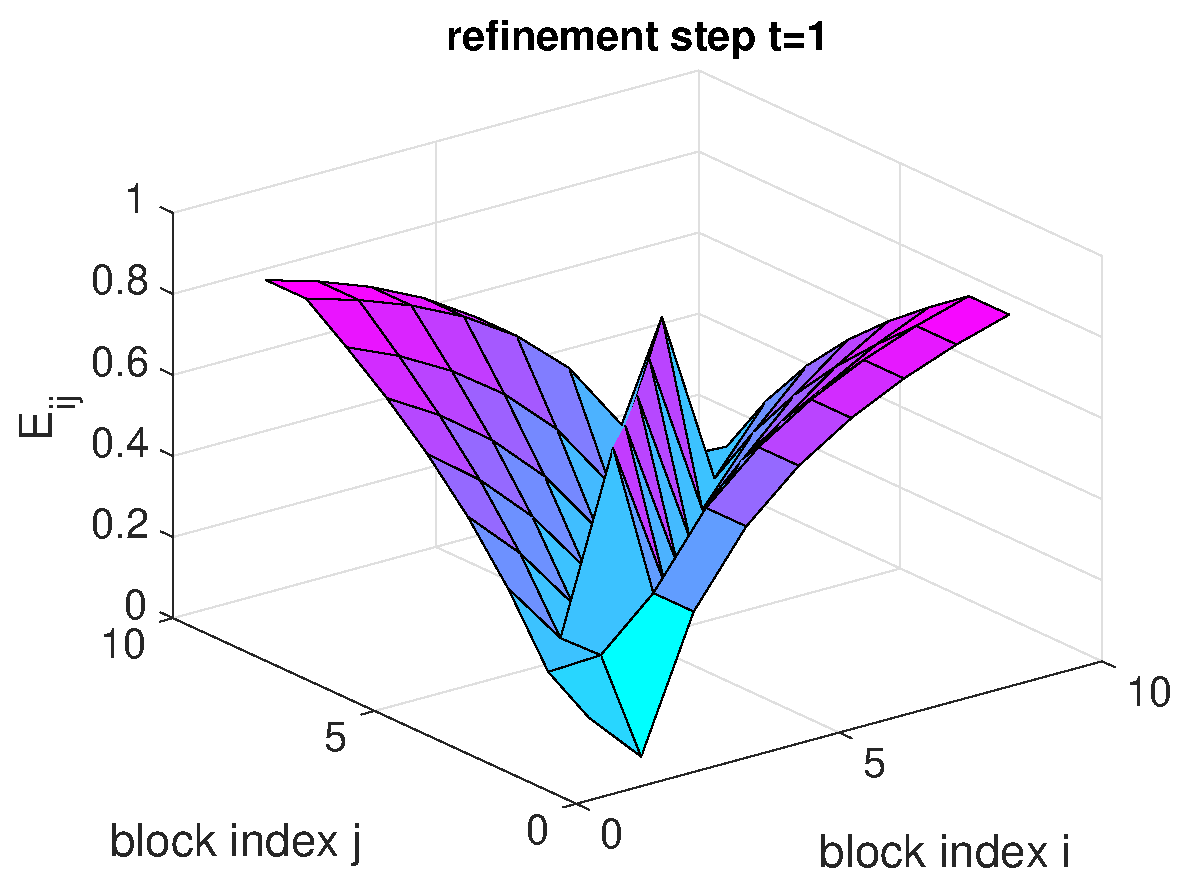
\includegraphics[width=0.475\linewidth]{figures/9times9_Z1_Error_t1.eps}
% 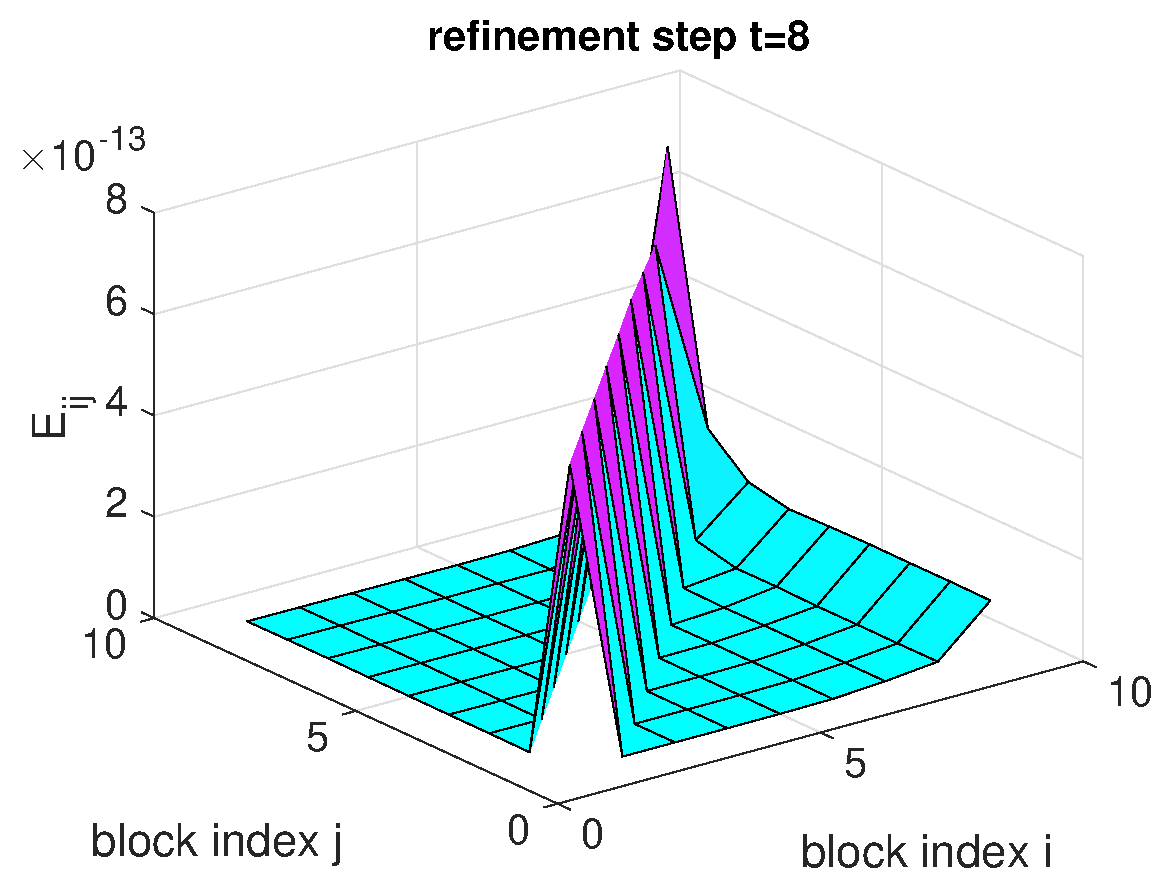
\includegraphics[width=0.475\linewidth]{figures/9times9_Z1_Error_t8.eps}\\[1ex]
% 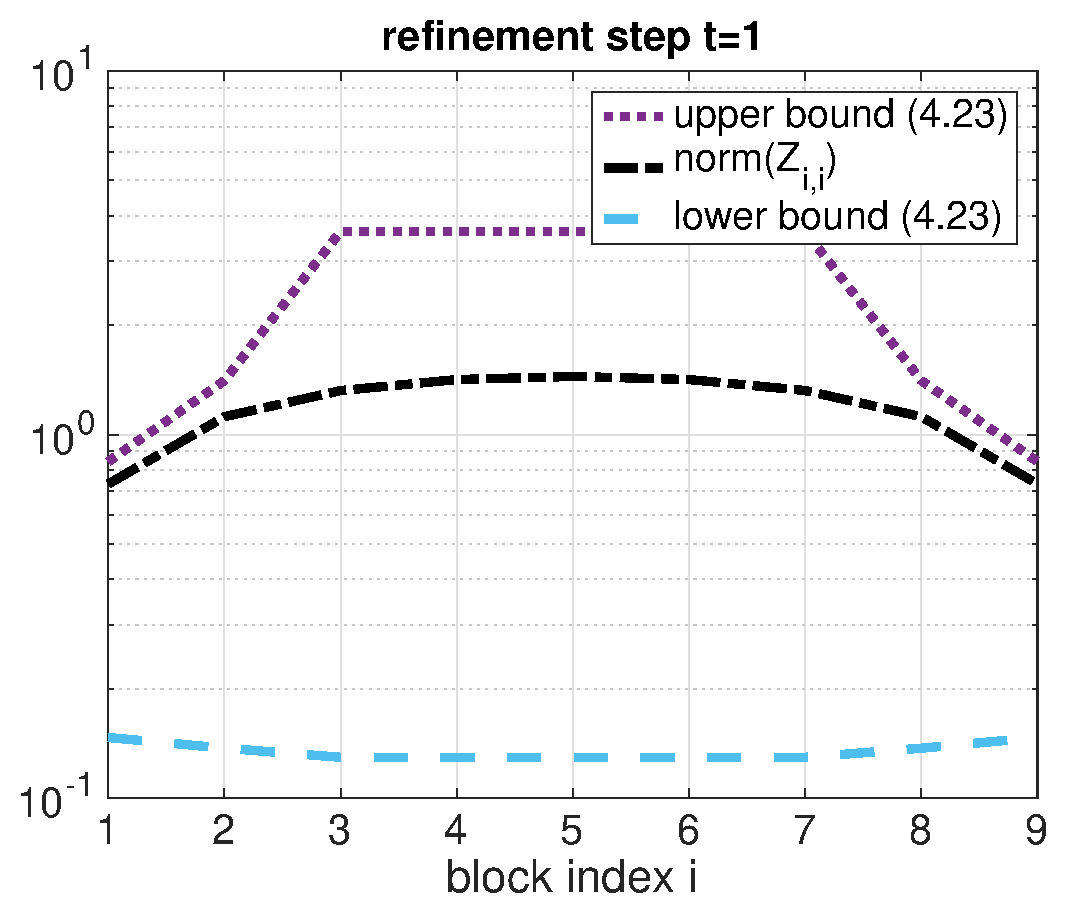
\includegraphics[width=0.475\linewidth]{figures/9times9_Z1_Bounds_t1.eps}
% 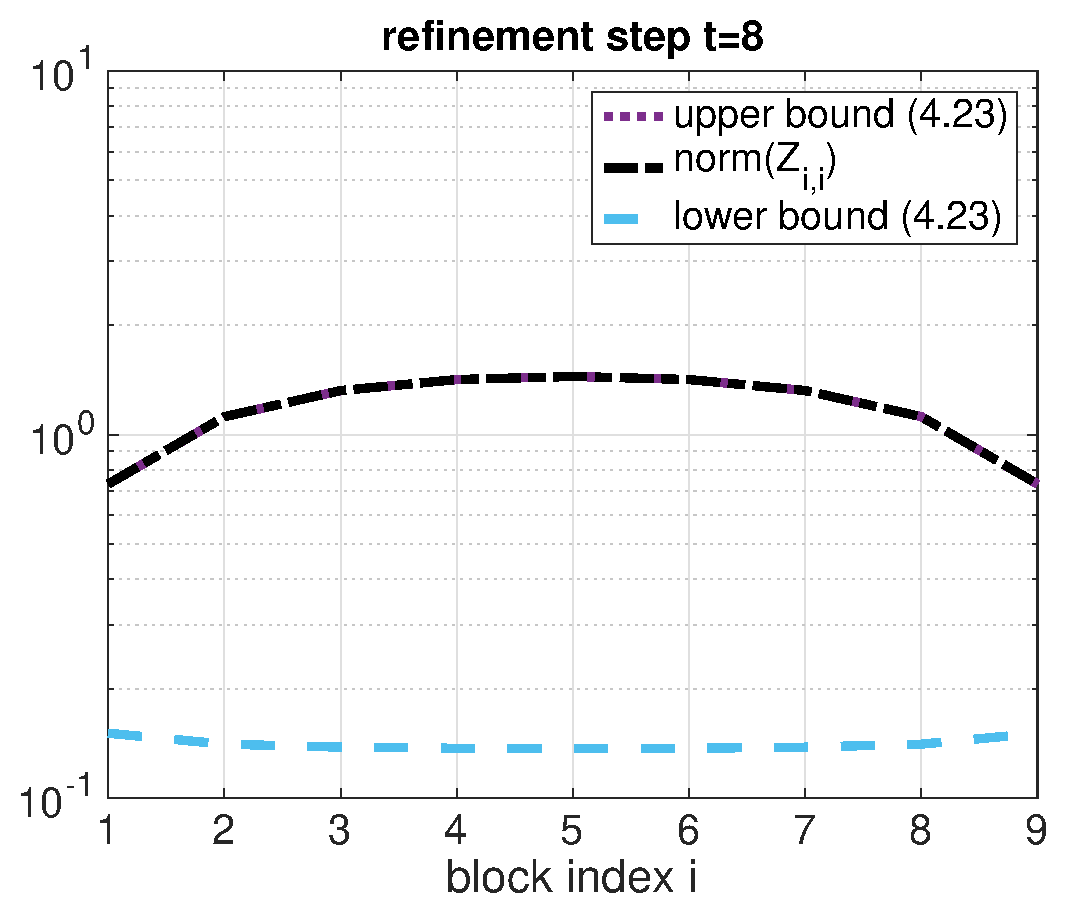
\includegraphics[width=0.475\linewidth]{figures/9times9_Z1_Bounds_t8.eps}
% %\includegraphics[width=0.475\linewidth]{figures/9times9_Z1_up-off-Bounds.eps}
% %\includegraphics[width=0.475\linewidth]{figures/9times9_Z1_low-off-Bounds.eps}
% \caption{Relative errors $\E^{\text{u}}_{ij}$ (top row), upper and lower bounds on $\|\Z_{ii}\|_2$ (bottom row) for the matrix $A$ of Example~\ref{ex:BDiDo:symm}.}
% \label{fig:BDiDo:ex:symm}
% \end{figure}
%
\begin{figure}[h!]
\vspace{-0.9em}
\hspace{-1cm}
\centering
\hspace*{2em}
\begin{minipage}[t]{0.48\linewidth}
\centering
\includegraphics[width=0.99\linewidth]{figures/9times9_Z1_Error_t1.eps}
\end{minipage}
%
\begin{minipage}[t]{0.48\linewidth}
\includegraphics[width=0.99\linewidth]{figures/9times9_Z1_Error_t8.eps}
\end{minipage}
\\\vspace*{0.8em}
\begin{minipage}[t]{0.48\linewidth}
\centering
\includegraphics[width=0.99\linewidth]{figures/9times9_Z1_Bounds_t1.eps}
\end{minipage}
%
\begin{minipage}[t]{0.48\linewidth}
\includegraphics[width=0.99\linewidth]{figures/9times9_Z1_Bounds_t8.eps}
\end{minipage}
\caption{Relative errors $\E^{\text{u}}_{ij}$ (top row), upper and lower bounds on $\|\Z_{ii}\|_2$ (bottom row) for the matrix $A$ of Example~\ref{ex:BDiDo:symm}.}
\label{fig:BDiDo:ex:symm}
\end{figure}
}% textrm
\end{example}

\newpage
\begin{example}\label{ex:BDiDo:nonsym1}{\textrm
Let $\A$ be the nonsymmetric block Toeplitz matrix of the form
\eqref{eq:BDiDo:kronA} with
$\T=\textnormal{tridiag}(-110,209.999,-99.999)\in\mathbb{R}^{9\times 9}$, i.e.,
$\A$ again takes the form \eqref{eq:BDiDo:blocktridiag} with
$\A_i=\textnormal{tridiag}(-110,419.999,-99.999)$,
$\B_i=\textnormal{diag}(-110)$, and $\C_i=\textnormal{diag}(-99.999)$. The
condition number in this case is $\kappa_2(\A)=57.5725$,  and for the computed
matrix $\Z$ we obtain $\|\Z\A-\I\|_2=1.5151\times 10^{-10}$.

The top row of \textnormal{Figure~\ref{fig:BDiDo:ex:nonsym1}} shows the
relative errors for the refinement steps $t=1$ and $t=8$. We observe that for
this nonsymmetric example the upper bounds are not as accurate as those given
in the symmetric case, producing a maximal relative error at refinement step
$t=8$ on the order $10^{-3}$. The bottom row of
\textnormal{Figure~\ref{fig:BDiDo:ex:nonsym1}} shows the upper and lower bounds
\eqref{eq:BDiDo:diagboundsiter} as well as the values $\|\Z_{ii}\|_2$ for
$i=1,\dots,9$, and refinement steps $t=1$ and $t=8$. Again we can observe that
while we obtain a reasonable approximation in the upper bounds on
$\|\Z_{ii}\|_2$ for $t=8$, the lower bounds almost do not improve by
the iterative refinement process. The maximal relative errors in the upper and
lower bounds and all refinement steps is shown in the following table:
%
%The maximal error of
%the lower bounds for the diagonal block entries of $Z$ in the maximal refinement step is again on the order %$10^{-1}$; see Table \ref{tab:errorA2}.
%
\begin{table}[h!]\scriptsize\centering
\begin{tabular}{c c c c c c c c c}
\hline
  t & 1 & 2 & 3 & 4 & 5 & 6 & 7 & 8 \\
$\max_{ij}\E^{u}_{ij}$ &  $0.88856$ & $ 0.70640$ & $0.46700$ &  $0.25859$ & $0.12442$ & $0.05378$ &  $0.02140$ &  $0.00824$\\
$\max_i \E^{l}_{i}$ & $0.90934$ & $0.90768$ & $0.90652$ & $0.90411$ & $0.90411$ & $0.90411$ &  $0.90411$ &  $0.90411$\\
\hline
\end{tabular}
%\caption{Values of the maximum relative errors for the matrix $A$ of Example 2.2 and  different values of $t$.}
%\label{tab:errorA2}
\end{table}
%\newpage
% \begin{figure}[h!]
% \centering
% % \includegraphics[width=0.475\linewidth]{figures/9times9_Z2_Error_t1.eps}
% % \includegraphics[width=0.475\linewidth]{figures/9times9_Z2_Error_t8.eps}\\[1ex]
% % \includegraphics[width=0.475\linewidth]{figures/9times9_Z2_Bounds_t1.eps}
% % \includegraphics[width=0.475\linewidth]{figures/9times9_Z2_Bounds_t8.eps}
% \includegraphics[scale=0.17]{figures/9times9_Z2_Error_t1.eps}
% \includegraphics[scale=0.17]{figures/9times9_Z2_Error_t8.eps}\\[1ex]
% \includegraphics[scale=0.17]{figures/9times9_Z2_Bounds_t1.eps}
% \includegraphics[scale=0.17]{figures/9times9_Z2_Bounds_t8.eps}
% \caption{Relative errors $\E^{\text{u}}_{ij}$ (top row), and upper and lower bounds on $\|\Z_{ii}\|_2$ (bottom row) for the matrix $\A$ of Example~\ref{ex:BDiDo:nonsym1}.}
% \label{fig:BDiDo:ex:nonsym1}
% \end{figure}
%
\begin{figure}[h!]
\vspace{-1.1em}
\hspace{-1cm}
\centering
\hspace*{2em}
\begin{minipage}[t]{0.48\linewidth}
\centering
\includegraphics[width=0.99\linewidth]{figures/9times9_Z2_Error_t1.eps}
\end{minipage}
%
\begin{minipage}[t]{0.48\linewidth}
\includegraphics[width=0.99\linewidth]{figures/9times9_Z2_Error_t8.eps}
\end{minipage}
\\%\vspace*{0.1em}
\begin{minipage}[t]{0.48\linewidth}
\centering
\includegraphics[width=0.99\linewidth]{figures/9times9_Z2_Bounds_t1.eps}
\end{minipage}
%
\begin{minipage}[t]{0.48\linewidth}
\includegraphics[width=0.99\linewidth]{figures/9times9_Z2_Bounds_t8.eps}
\end{minipage}
\caption{Relative errors $\E^{\text{u}}_{ij}$ (top row), and upper and lower bounds on $\|\Z_{ii}\|_2$ (bottom row) for the matrix $\A$ of Example~\ref{ex:BDiDo:nonsym1}.}
\label{fig:BDiDo:ex:nonsym1}
\end{figure}
}\end{example}

\newpage

\begin{example}\label{ex:BDiDo:nonsym2}{\textrm
We now consider the  nonsymmetric block tridiagonal matrix
\[\A~=(\R\otimes \I)(\T\otimes \I+ \I\otimes~\T) \;\;\in\;\;\mathbb{R}^{81\times 81},\]
where $\T$ is given as in \textnormal{Example~\ref{ex:BDiDo:symm}}, and
$\R\in\mathbb{R}^{9\times 9}$ is a random diagonal matrix with nonzero integer
entries between $0$ and $10$ and constructed in \textnormal{\texttt{MATLAB}}
with the command \textnormal{\texttt{\R = diag(ceil(10*rand(9,1)))}}. Thus,
$\A$ is of the form \eqref{eq:BDiDo:blocktridiag} with random tridiagonal
Toeplitz matrices $\A_i$, and random constant diagonal matrices $\B_i$ and
$\C_i$ for all $i$. For this matrix we have $\kappa_2(\A)=489.7595$, and the
computed matrix $\Z$ yields $\|\Z\A-\I\|_2=2.8328\times 10^{-10}$. The relative
errors in the bounds are shown in \textnormal{Figure~\ref{fig:BDiDo:ex:nonsym2}} and in the following table:
%
\begin{table}[h!]\scriptsize\centering
\begin{tabular}{c c c c c c c c c}
\hline
%\cline{2-5}
 t & 1 & 2 & 3 & 4 & 5 & 6 & 7 & 8 \\
 $\max_{ij}\E^{u}_{ij}$ &  $0.84477$ & $0.63381$  &  $0.39537$ &  $0.20898$ & $0.09595$ &  $0.03780$ &  $0.01109$ &  $9.739\times 10^{-13}$\\
 $\max_{i}\E^{l}_{i}$ &  $0.91039$ & $0.90877$ & $0.90765$ & $0.90529$ & $0.90529$ &  $0.90529$ &  $0.90529$ &  $0.90529$\\
  \hline
\end{tabular}
%\caption{Values of the maximum relative errors for the matrix $A$ of Example 2.3 and  different values of $t$.}
%\label{tab:errorA3}
\end{table}
%

%\newpage
% \begin{figure}[h!]
% \centering
% % \includegraphics[width=0.475\linewidth]{figures/9times9_Z3_Error_t1.eps}
% % \includegraphics[width=0.475\linewidth]{figures/9times9_Z3_Error_t8.eps}\\[1ex]
% % \includegraphics[width=0.475\linewidth]{figures/9times9_Z3_Bounds_t1.eps}
% % \includegraphics[width=0.475\linewidth]{figures/9times9_Z3_Bounds_t8.eps}
% \includegraphics[scale=0.18]{figures/9times9_Z3_Error_t1.eps}
% \includegraphics[scale=0.18]{figures/9times9_Z3_Error_t8.eps}\\[1ex]
% \includegraphics[scale=0.18]{figures/9times9_Z3_Bounds_t1.eps}
% \includegraphics[scale=0.18]{figures/9times9_Z3_Bounds_t8.eps}
% \caption{Relative errors $\E^{\text{u}}_{ij}$ (top row), and upper and lower bounds on $\|\Z_{ii}\|_2$ (bottom row) for the matrix $\A$ of Example~\ref{ex:BDiDo:nonsym2}.}
% \label{fig:BDiDo:ex:nonsym2}
% \end{figure}
%
\vspace*{1em}
\begin{figure}[h!]
\hspace{-1cm}
\centering
\hspace*{2em}
\begin{minipage}[t]{0.48\linewidth}
\centering
\includegraphics[width=0.99\linewidth]{figures/9times9_Z3_Error_t1.eps}
\end{minipage}
%
\begin{minipage}[t]{0.48\linewidth}
\includegraphics[width=0.99\linewidth]{figures/9times9_Z3_Error_t8.eps}
\end{minipage}
\\\vspace{3em}
\begin{minipage}[t]{0.48\linewidth}
\centering
\includegraphics[width=0.99\linewidth]{figures/9times9_Z3_Bounds_t1.eps}
\end{minipage}
%
\begin{minipage}[t]{0.48\linewidth}
\includegraphics[width=0.99\linewidth]{figures/9times9_Z3_Bounds_t8.eps}
\end{minipage}
\caption{Relative errors $\E^{\text{u}}_{ij}$ (top row), and upper and lower bounds on $\|\Z_{ii}\|_2$ (bottom row) for the matrix $\A$ of Example~\ref{ex:BDiDo:nonsym2}.}
\label{fig:BDiDo:ex:nonsym2}
\end{figure}
}\end{example}

\newpage

\begin{example}\label{ex:BDiDo:nonsym3}{\textrm
Finally, we consider the nonsymmetric block tridiagonal matrix
\begin{equation*}
\A=\\(\R\otimes \I)\tridiag(\tridiag(-0.01,-2,1),\tridiag(-2,10,-2),\tridiag(-0.01,-2,1)),
\end{equation*}
with $\A\in\mathbb{R}^{81\times 81}$, and where $\R\in\mathbb{R}^{9\times 9}$
is a random diagonal matrix constructed as in
\textnormal{Example~\ref{ex:BDiDo:nonsym2}}.
In this case $\A$ takes the form \eqref{eq:BDiDo:blocktridiag} with $\A_i$,
$\B_i$ and $\C_i$ random tridiagonal Toeplitz matrices with integer entries
for all $i$. For this matrix we have $\kappa_2(\A)=58.478$, and
$\|\Z\A-\I\|_2=2.7962\times 10^{-10}$. The relative errors in the bounds
are shown in \textnormal{Figure~\ref{fig:BDiDo:ex:nonsym3}} and the following
table:
%
\begin{table}[h!]\scriptsize\centering
\begin{tabular}{c c c c c c c c c}
\hline
 t & 1 & 2 & 3 & 4 & 5 & 6 & 7 & 8 \\
 $\max_{ij}\E^{u}_{ij}$ &  $0.84477$ & $0.63381$ & $0.39537$ & $0.20898$ & $0.09595$ & $0.03780$ &  $0.01109$ & $7.142\times 10^{-13}$\\
 $\max_{i}\E^{l}_{i}$ &  $0.91039$ & $0.90877$ & $0.90765$ & $0.90529$ & $0.90529$ & $0.90529$ &  $0.90529$ & $0.90529$\\
  \hline
\end{tabular}
%\caption{Values of the maximum relative errors for the matrix $A$ of Example 2.4 and  different values of $t$.}
%\label{tab:errorA4}
\end{table}
%
%\newpage
% \begin{figure}[h!]
% \centering
% \includegraphics[width=0.475\linewidth]{figures/9times9_Z4_Error_t1b.eps}
% \includegraphics[width=0.475\linewidth]{figures/9times9_Z4_Error_t8b.eps}\\[1ex]
% \includegraphics[width=0.475\linewidth]{figures/9times9_Z4_Bounds_t1b.eps}
% \includegraphics[width=0.475\linewidth]{figures/9times9_Z4_Bounds_t8b.eps}
% \caption{Relative errors $\E^{\text{u}}_{ij}$ (top row), and upper and lower bounds on $\|\Z_{ii}\|_2$ (bottom row) for the matrix $\A$ of Example~\ref{ex:BDiDo:nonsym3}.}
% \label{fig:BDiDo:ex:nonsym3}
% \end{figure}
\vspace*{2em}
\begin{figure}[h!]
%\vspace{-1.1em}
\hspace{-1cm}
\centering
\hspace*{2em}
\begin{minipage}[t]{0.48\linewidth}
\centering
\includegraphics[width=0.99\linewidth]{figures/9times9_Z4_Error_t1.eps}
\end{minipage}
%
\begin{minipage}[t]{0.48\linewidth}
\includegraphics[width=0.99\linewidth]{figures/9times9_Z4_Error_t8.eps}
\end{minipage}
\\\vspace{4em}
\begin{minipage}[t]{0.48\linewidth}
\centering
\includegraphics[width=0.99\linewidth]{figures/9times9_Z4_Bounds_t1.eps}
\end{minipage}
%
\begin{minipage}[t]{0.48\linewidth}
\includegraphics[width=0.99\linewidth]{figures/9times9_Z4_Bounds_t8.eps}
\end{minipage}
\caption{Relative errors $\E^{\text{u}}_{ij}$ (top row), and upper and lower bounds on $\|\Z_{ii}\|_2$ (bottom row) for the matrix $\A$ of Example~\ref{ex:BDiDo:nonsym3}.}
\label{fig:BDiDo:ex:nonsym3}
\end{figure}
}\end{example}

\newpage

% \subsection{Eigenvalue Inclusion Sets}
% \label{BDiDo:numerics:sets}
% %
We continue by providing a set of numerical illustrations of of the newly
proposed eigenvalue inclusion sets, $G_i^{\text{new}}$, which are a consequence
of Corollary~\ref{cor:BDiDo:inclusion}. We consider different matrices
$\A=[\A_{ij}]$, and we compute the boundaries of the sets $G_i^{\text{new}}$ and
$G_i^{\text{FV}}$ for all $i\leq n$, i.e., the curves for $z\in {\mathbb C}$
where
\begin{equation*}
\sum_{\atopfrac{j=1}{j\neq i}}^{n}\| (\A_{ii}-z \I)^{-1} \A_{ij} \|=1,\text{ and }
%\quad i,j\in\{1,2\},\quad i\neq j,\\
\sum_{\atopfrac{j=1}{j\neq i}}^{n}\| (\A_{ii}-z \I)^{-1}\|\| \A_{ij} \|=1,
\quad i,j\in\{1,\ldots,n\},\quad i\neq j,
\end{equation*}
%
respectively.

\begin{example}\label{ex:BDiDo:inclusion}{\textrm
We first consider the symmetric matrix
\begin{equation}\label{eq:BDiDo:ELNmatrix1}
\A=
\left[ \begin{array}{rr|rr}
4	& -2	& -1 & 1	\\
-2	&	4	&  0 & -1	\\ \hline
-1	& 0	&	4	&-2	\\
1	& -1	& -2	& 4
\end{array} \right]
=
\left[ \begin{array}{c|c}
\A_{11}	& \A_{12}	\\ \hline
\A_{21}	& \A_{22}
\end{array} \right],
\end{equation}
which has the eigenvalues $1.4586$, $2.3820$, $4.6180$, and $7.5414$
(computed in \textnormal{\texttt{MATLAB}} and rounded to five significant
digits). \textnormal{Figure~\ref{fig:BDiDo:ex:inclusion1}}
shows the boundaries of the corresponding sets $G_i^{\text{new}}$ and
$G_i^{\text{FV}}$ for $i=1,2$, i.e., the curves for $z\in {\mathbb C}$ where
%
%\begin{eqnarray*}
%&& \| (A_{ii}-z I)^{-1} A_{ij} \|=1,\quad \| A_{ij} (A_{ii}-z I)^{-1}  \|=1,
%\quad i,j\in\{1,2\},\quad i\neq j,\\
%&&\| (A_{ii}-z I)^{-1}\|\| A_{ij} \|=1,
%\quad i,j\in\{1,2\},\quad i\neq j,
%\end{eqnarray*}
%
\begin{equation*}
\| (\A_{ii}-z \I)^{-1} \A_{ij} \|=1,\text{ and }
%\quad i,j\in\{1,2\},\quad i\neq j,\\
\| (\A_{ii}-z \I)^{-1}\|\| \A_{ij} \|=1,
\quad i,j\in\{1,2\},\quad i\neq j,
\end{equation*}
%
respectively. Clearly, the sets $G_i^{\text{new}}$ give tighter inclusion
regions for the eigenvalues than the sets $G_i^{\text{FV}}$ as well as the
usual Gershgorin circles for the matrix $\A$, which are given by the two
circles centered at $z=4$ of radius~3 and~4.

\begin{figure}[h!]
\centering
\vspace*{-0.4cm}
\includegraphics[width=0.49\linewidth]{figures/Example415_a1}
\includegraphics[width=0.49\linewidth]{figures/Example415_a2}
\vspace*{-0.5cm}
\caption{Eigenvalue inclusion regions obtained from the sets
$G_i^{\text{new}}$ and $G_i^{\text{FV}}$ for the matrix \eqref{eq:BDiDo:ELNmatrix1} of Example~\ref{ex:BDiDo:inclusion}.}
\label{fig:BDiDo:ex:inclusion1}
\end{figure}

We next consider the nonsymmetric matrix
\begin{equation}\label{eq:BDiDo:ELNmatrix2}
\A=
\left[ \begin{array}{rr|rr}
4	& -2	& -0.5 & 0.5	\\
-2	&	5	&  -1.4 & -0.5	\\ \hline
-0.5	& 0	&	4	&-2	\\
0.5	& -0.5	& -2	& 4
\end{array} \right]
=
\left[ \begin{array}{c|c}
\A_{11}	& \A_{12}	\\ \hline
\A_{21}	& \A_{22}
\end{array} \right],
\end{equation}
which has the eigenvalues $1.6851$, $2.5959$, $6.2263$, and $6.4927$. As shown
in \textnormal{Figure~\ref{fig:BDiDo:ex:inclusion2}}, the sets
$G_i^{\text{new}}$ again give tighter inclusion regions than the sets
$G_i^{\text{FV}}$ as well as the usual Gershgorin circles.
%
\begin{figure}[tbph]
\centering
\vspace*{-0.4cm}
\includegraphics[width=0.49\linewidth]{figures/Example415_b1}
\includegraphics[width=0.49\linewidth]{figures/Example415_b2}
\vspace*{-0.5cm}
\caption{Eigenvalue inclusion regions obtained from the sets
$G_i^{\text{new}}$ and $G_i^{\text{FV}}$ for the matrix \eqref{eq:BDiDo:ELNmatrix2} of Example~\ref{ex:BDiDo:inclusion}.}
\label{fig:BDiDo:ex:inclusion2}
\end{figure}
}\end{example}

% In the next example, we show the inclusion sets for larger matrices.

% \begin{example}\label{ex:BDiDo:inclusion2}{\textrm
% Consider the symmetric block tridiagonal matrix $\A$ given by
% \[
% \A~=\I_9\otimes~\T_1+\T_2\otimes \I_5 \;\;\in\;\;\mathbb{R}^{45\times 45},
% \]
% where $\T_1=\textnormal{tridiag}(-2,2,-2) \in {\mathbb R}^{9\times 9}$ and
% $\T_2=\textnormal{tridiag}(-0.5,2,-0.5)\in {\mathbb R}^{5\times 5}$.
% Thus, $\A$ is of the form \eqref{eq:BDiDo:blocktridiag} with constant
% tridiagonal Toeplitz matrices $\A_i=\textnormal{tridiag}(-2,4,-2)\in {\mathbb R}^{9\times 9}$ and constant diagonal matrices $\B_i=\C_i=\textnormal{diag}(-0.5)\in {\mathbb R}^{9\times 9}$ for all $i$; its structure is
% shown in the left part of \textnormal{Figure~\ref{fig:BDiDo:ex:inclusion2_b}}.
% % and has the eigenvalues\td{\textbf{add:}eigenvalues of this matrix.}
% %(computed in \texttt{MATLAB} and rounded to five significant digits).
% %
%
% The boundaries of the corresponding sets $G_i^{\text{new}}$ and $G_i^{FV}$ for
% $i=1,\ldots,9$ are shown on the left side of
% \textnormal{Figure~\ref{fig:BDiDo:ex:inclusion2}}. The sets $G_i^{\text{new}}$
% give the same inclusion regions for the
% eigenvalues than the sets $G_i^{\text{FV}}$ since the off-diagonal blocks are
% diagonal (both inclusion regions are tighter than the usual
% Gershgorin circles), nevertheless if we now make a small perturbation to the
% off-diagonal blocks, mainly we make the upper right corner of each block in the
% first block row and the lower left entry of each block in the first block
% column equal to $0.5$ - see the right side of \textnormal{Figure~\ref{fig:BDiDo:ex:inclusion2_b}}, the sets are no longer
% equal; even though the matrix is still symmetric - see the right side of
% \textnormal{Figure~\ref{fig:BDiDo:ex:inclusion2}}.
% %
% \begin{figure}[h!]
% \vspace*{-1em}
% \centering
% \includegraphics[width=0.49\linewidth]{figures/Example417_b1}
% \includegraphics[width=0.49\linewidth]{figures/Example417_a1}
% \vspace{-1em}
% \caption{Eigenvalue inclusion regions obtained from the sets
% $G_i^{\text{new}}$ and $G_i^{\text{FV}}$ of Example~\ref{ex:BDiDo:inclusion2}.}
% \label{fig:BDiDo:ex:inclusion2}
% \end{figure}
% %
% \begin{figure}[h!]
% \centering
% \includegraphics[width=0.4\linewidth]{figures/Example417_b2}
% \includegraphics[width=0.4\linewidth]{figures/Example417_a2}
% \caption{Sparsity pattern of the matrices of Example~\ref{ex:BDiDo:inclusion2}.}
% \label{fig:BDiDo:ex:inclusion2_b}
% \end{figure}
% %
% }\end{example}

% \begin{example}\label{ex:BDiDo:inclusion3}{\textrm
% Consider the  nonsymmetric block tridiagonal matrix $\A$ as in Example~\ref{ex:BDiDo:symm}, i.e.,
% \[\A~=(\R\otimes \I)(\T\otimes \I+ \I\otimes~\T) \;\;\in\;\;\mathbb{R}^{81\times 81},\]
% where $\T=\textrm{tridiag}(-1,2,-1) \in {\mathbb R}^{9\times 9}$ and
% $\R\in\mathbb{R}^{9\times 9}$ is a random diagonal matrix with nonzero integer
% entries between $0$ and $10$ and constructed in \texttt{MATLAB} with the command
% \texttt{\R = diag(ceil(10*rand(9,1)))}. Thus, $\A$ is of the form
% \eqref{eq:BDiDo:blocktridiag} with random tridiagonal Toeplitz matrices
% $\A_i$, and random constant diagonal matrices $\B_i$ and $\C_i$ for all $i$ and
% has the eigenvalues\td{\textbf{add:}eigenvalues of this matrix.}
% (computed in \texttt{MATLAB} and rounded to five significant digits).
% %
% The boundaries of the corresponding sets $G_i^{\text{new}}$ and $G_i^{FV}$ for
% $i=1,\ldots,9$ are shown on Figure~\ref{fig:BDiDo:ex:inclusion3}.
% %
% \begin{figure}[h!]
% \centering
% \includegraphics[width=0.49\linewidth]{figures/Example416a}
% \includegraphics[width=0.49\linewidth]{figures/Example416b}
% \caption{Eigenvalue inclusion regions obtained from the sets
% $G_i^{\text{new}}$ and $G_i^{\text{FV}}$ of Example~\ref{ex:BDiDo:inclusion3} for two different ramdom matrices $\R$.}
% \label{fig:BDiDo:ex:inclusion2}
% \end{figure}
% %
% The sets $G_i^{\text{new}}$ give the same inclusion regions for the
% eigenvalues than the sets $G_i^{\text{FV}}$ since the off diagonal blocks are still diagonal, nevertheless both inclusion regions are tighter than the usual Gershgorin circles.
% }\end{example}
%
We now present an example of the inclusion sets for the eigenvalues of a  matrix
\begin{equation}\label{eq:BDiDo:ConvDiffMat}
\A=\left[
  \begin{array}{ccc}
             \matAHhat       & \e_{m}\otimes\matBH   &    0            \\
    \e_{m}^{\Tr}\otimes\matC  &   \matA      & \e_{1}^{\Tr}\otimes\matB \\
                   0         & \e_{1}\otimes\matCh &        \matAhhat  \\
  \end{array}
\right]\;\in\;{\mathbb R}^{N(2m+1)\times N(2m+1)},
\end{equation}
obtained, for example, from a Shishkin mesh discretization of the 2D convection-diffusion problems of type \eqref{eq:2D:2Dbvp} studied in Chapter~\ref{ch:2D}.

% \newpage
\begin{example}\label{ex:BDiDo:inclusionconvdiff1}{\textrm
Consider the  nonsymmetric block tridiagonal matrix
\begin{equation}\label{eq:BDiDo:ConvDiffMat1}
\A=\left[
  \begin{array}{ccc}
 \matA  & \matB  &      0     \\
     \matC  &   \matA &  \matB     \\
      0     & \matC  &  \matA  \\
  \end{array}
\right]\;\in\;{\mathbb R}^{15 \times 15},
\end{equation}
where $\matA=\mathrm{tridiag}(-36,108,-36)\in\mathbb{R}^{5\times5}$, $\matB=\mathrm{diag}(-16)\in\mathbb{R}^{5\times5}$ and
$\matC=\mathrm{diag}(-20)~\in~\mathbb{R}^{5\times5}$, i.e., we have a matrix of type \eqref{eq:BDiDo:ConvDiffMat} with $N=5$, $m=1$ and $\matAHhat=\matAhhat=\matA$, $\matBH=\matB$, and  $\matCh=\matC$. \textnormal{Figure~\ref{fig:BDiDo:ex:inclusion3}}
shows the $15$ eigenvalues computed in \textnormal{\texttt{MATLAB}} and rounded to five significant digits as well as the boundaries of the corresponding sets $G_i^{\text{new}}$, and $G_i^{\text{FV}}$ for $i=1,2,3$.
%
\begin{figure}[tbph]
\centering
\vspace*{-0.4cm}
\includegraphics[width=0.49\linewidth]{figures/Example416_b1}
\includegraphics[width=0.49\linewidth]{figures/Example416_b2}
% \vspace*{-0.5cm}
\caption{Eigenvalue inclusion regions obtained from the sets
$G_i^{\text{new}}$ and $G_i^{\text{FV}}$ for the matrix \eqref{eq:BDiDo:ConvDiffMat1} of Example~\ref{ex:BDiDo:inclusionconvdiff1}.}
\label{fig:BDiDo:ex:inclusion3}
\end{figure}

The figure shows that  sets $G_i^{\text{new}}$ give the same inclusion regions
for the eigenvalues than the sets $G_i^{\text{FV}}$ (both inclusion regions are tighter than the usual Gershgorin circles); this is to be expected since the off-diagonal blocks are multiples of the identity matrix and the sets $G_i^{\text{new}}$ reduce to the sets $G_i^{\text{FV}}$. However, by changing the structure of the
off-diagonal blocks (we make the upper right corner of each upper off-diagonal block and the lower left entry of each lower off-diagonal block equal to~$10$), the eigenvalues do not shift much, nevertheless, the sets are no longer equal and once again the new sets $G_i^{\text{new}}$ present much tighter inclusion regions than the sets $G_i^{\text{FV}}$ - see the right side of \textnormal{Figure~\ref{fig:BDiDo:ex:inclusion3}}
}\end{example}

\begin{example}\label{ex:BDiDo:inclusionconvdiff2}{\textrm
Consider the  nonsymmetric block tridiagonal matrix \eqref{eq:BDiDo:ConvDiffMat1} from \textnormal{Example~\ref{ex:BDiDo:inclusionconvdiff1}}
where $\matA=\mathrm{tridiag}(-36,108,-36)\in\mathbb{R}^{5\times5}$, but now we choose the off-diagonal blocks $\matB$ and $\matC$ as $5\times5$ diagonal matrices with random positive integer entries between $0$ and $9$ using the \textnormal{\texttt{MATLAB}} command \textnormal{\texttt{diag(floor(10*rand(5,1)))}}. \textnormal{Figure~\ref{fig:BDiDo:ex:inclusion4}} once again
shows the $15$ eigenvalues as well as the boundaries of the corresponding sets $G_i^{\text{new}}$, and $G_i^{\text{FV}}$ for $i=1,2,3$.
%
\begin{figure}[tbph]
\centering
\vspace*{-0.5cm}
\includegraphics[width=0.9\linewidth]{figures/Example417}
\vspace*{-0.7cm}
\caption{Eigenvalue inclusion regions obtained from the sets
$G_i^{\text{new}}$ and $G_i^{\text{FV}}$ for the matrix \eqref{eq:BDiDo:ConvDiffMat1} of Example~\ref{ex:BDiDo:inclusionconvdiff2}.}
\label{fig:BDiDo:ex:inclusion4}
\end{figure}

\textnormal{Figure~\ref{fig:BDiDo:ex:inclusion4}} once again shows that sets $G_i^{\text{new}}$ present much tighter incusion regions than the sets $G_i^{\text{FV}}$.
In the context of convection diffusion equations, a coefficient matrix with the structure given by this example might correspond to having variable coefficients in equation~\eqref{eq:2D:2Dbvp} instead of constant ones, like it is the case for the matrix in Example~\ref{ex:BDiDo:inclusionconvdiff1}.
}\end{example}



\begin{example}\label{ex:BDiDo:inclusionconvdiff3}{\textrm
Consider the  nonsymmetric block tridiagonal matrix arising from the Shishkin mesh discretization of the convection-diffusion model problem \eqref{eq:2D:2Dbvp} with $\epsilon=10^{-4}$, using $16$ intervals in the $x$-direction and $8$ intervals in the $y$-direction (see next chapter) yielding a matrix of type \eqref{eq:BDiDo:ConvDiffMat} with $N=15$ and $m=7$. \textnormal{Figure~\ref{fig:BDiDo:ex:inclusion5}} shows the eigenvalues of the matrix as well as the boundaries of the corresponding sets $G_i^{\text{new}}$, and $G_i^{\text{FV}}$ for $i=1,\ldots,105$.
%
\begin{figure}[tbph]
\centering
\vspace*{-0.5cm}
\includegraphics[width=0.6\linewidth]{figures/Example418}
\vspace*{-0.2cm}
\caption{Eigenvalue inclusion regions obtained from the sets
$G_i^{\text{new}}$ and $G_i^{\text{FV}}$ for the matrix \eqref{eq:BDiDo:ConvDiffMat1} of Example~\ref{ex:BDiDo:inclusionconvdiff3}.}
\label{fig:BDiDo:ex:inclusion5}
\end{figure}
%
Just like it is the case for \textnormal{Example~\ref{ex:BDiDo:inclusionconvdiff1}}, the sets $G_i^{\text{new}}$ present the same inclusion regions than the sets $G_i^{\text{FV}}$. As we have discussed before, this is due to the constant-coefficient nature of the problem. Even though the eigenvalues appear clustered together in 4 tight clusters, the difference in magnitude between the eigenvalues, caused by the convection-domitated characteristic of the problem, makes the inclusion regions cover a much larger part of the complex plane than expected (notice the scale in \textnormal{Figure~\ref{fig:BDiDo:ex:inclusion5}}). Moreover, the regions grow as the problem becomes more convection dominated, making the inclusion sets not very informative in the case of real world problems. It is important to note, however, that a different subdivision of the blocks of \eqref{eq:BDiDo:ConvDiffMat} might lead to tighter inclusion regions for these type of problems, a task that remains to be explored.
}\end{example}

% All experiments were computed on a 13-inch \texttt{Apple MacBook} computer model Mid 2010 with a 2,4 GHz Intel Core 2 Duo processor equipped with \texttt{MATLAB} version R2015b.
To complete this chapter, we present the definition of \emph{column} block diagonal dominance of matrices in the following Appendix.

\begin{subappendices}
\section{Column Block Diagonal Dominance of Matrices}
\label{App:BDiDo:ColBDiDo}
According to Definition~\ref{def:BDiDo:bdd} in Section~\ref{BDiDo:bounds}, the
property of \emph{column} block diagonal dominance of matrices is defined as
follows:
\begin{definition}\label{def:App:colbdd}
Consider a matrix of the form
%
\begin{equation}\label{eq:app:blockmatrix}
\A=[\A_{ij}]\quad
\mbox{with blocks $\A_{ij}\in\mathbb{C}^{m\times m}$ for $i,j=1,\dots,n$.}
\end{equation}
%
The matrix $\A$ is called \emph{column block diagonally dominant} (with respect
to the matrix norm $\|\cdot\|$) when the diagonal blocks $\A_{jj}$ are
nonsingular, and
%
\begin{equation}\label{eq:app:blocdiagdom1}
\sum_{\atopfrac{i=1}{i\neq j}}^{n} \|\A_{ij}\A_{jj}^{-1}\| \leq 1,
\quad \text{for $j=1,\dots,n$}.
\end{equation}
%
If strict inequality holds in \eqref{eq:app:blocdiagdom1} then $\A$ is called
\emph{column block strictly diagonally dominant} (with respect to the matrix
norm $\|\cdot\|$).
\end{definition}

Now, restricting our attention to block tridiagonal matrices of the form
\eqref{eq:BDiDo:blocktridiag} and following the notation of that chapter, in
order to obtain analogous bounds for the norms of the inverses of a column
block diagonally dominant matrix we fist need to set $\B_0~=~\C_n~=~0$, and
define the \emph{new} quantities
%
\begin{eqnarray*}
\tilde{\tau}_i   &\equiv& \frac{\|\C_i\A_i^{-1}\|}{1-\|\B_{i-1}\A_i^{-1}\|},
\quad \text{for $i=1,\ldots,n$}, \\
\tilde{\mu}_i &\equiv& \frac{\|\B_{i-1}\A_i^{-1}\|}{1-\|\C_{i}\A_i^{-1}\|},
\quad \text{for $i=1,\ldots,n$}.
\end{eqnarray*}
%
The column block diagonal dominance of $\A$ then implies that
$0~\leq ~\tilde{\tau}_i\leq~1$ and $0~\leq~\tilde{\mu}_i~\leq~1$.
Using these quantities we obtain the following result.
%
\begin{thm}
Let $A$  be as in \eqref{eq:BDiDo:blocktridiag} and suppose that
$\A_i^{-1}$ as well as $\B_i^{-1}$ and $\C_i^{-1}$ for $i=1,\ldots,n-1$ exist.
Suppose in addition that $\A$ is column block diagonally dominant, and that
%
\begin{equation}\label{eq:app:blktridom_b}
\|\C_1\A_1^{-1}\|<1 \quad \mbox{and} \quad \|\B_{n-1}\A_n^{-1}\|<1.
\end{equation}
%
Then $\A^{-1}=[\Z_{ij}]$ with
%
\begin{align}
\|\Z_{ij}\| & \leq  \|\Z_{ii}\| \prod_{k=i+1}^{j}\tilde{\mu}_k,
\quad\text{for all $i<j$}, \label{eq:app:offdiagbound1}\\
\|\Z_{ij}\| & \leq  \|\Z_{ii}\|\;\,\prod_{k=j}^{i-1}\tilde{\tau}_k,
\qquad\text{for all $i>j$},\label{eq:app:offdiagbound2}
\end{align}
%
with $\mu_k$ and $\tau_k$ given by \eqref{eq:BDiDo:mu} and \eqref{eq:BDiDo:tau}. Moreover, for $i=1,\dots,n$,
%
\begin{equation}\label{eq:app:diagbounds}
\frac{\|\I\|}
{\|\A_i\|+\tilde{\tau}_{i-1}\|\B_{i-1}\|+\tilde{\mu}_{i+1}\|\C_{i}\|}
\leq
\|\Z_{ii}\|
\leq
\frac{\|\I\|}
{\|\A_i^{-1}\|^{-1}-\tilde{\tau}_{i-1}\|\B_{i-1}\|-\tilde{\mu}_{i+1}\|\C_i\|},
\end{equation}
%
provided that the denominator of the upper bound is larger than zero,
and where we set $\B_0=\C_n=0$, and $\tilde{\tau}_0=\tilde{\mu}_{n+1}=0$.
\end{thm}

\begin{proof}
The proof of this theorem is completely analogous to the one of
Theorem~\ref{thm:BDiDo:blockbounds} for row block diagonally dominant matrices
when the necessary adaptations are made, i.e., by performing the following
changes:
%
\begin{itemize}

\item Formulate Lemma~\ref{lem:BDiDo:sequences} for the matrices $\X_i$ and
$\V_i$, showing that the sequence $\{\|\X_i\|\}_{i=1}^n$ is strictly increasing
while the sequence $\{\|\V_i\|\}_{i=1}^n$ is strictly decreasing.

\item Formulate Lemma~\ref{lem:BDiDo:nonsing} for the matrices
$\tilde{\L}_1=\tilde{\T}_1=\C_1\A_1^{-1}$, $\tilde{\T}_2=\I-\tilde{\T}_1\B_1\A_2^{-1}$,
$\tilde{\L}_i = \C_{i}\A_i^{-1}\tilde{\T}_i^{-1}$, and
$\tilde{\T}_i = \I-\tilde{\L}_{i-1}\B_{i-1}\A_i^{-1}$. Analogously for $\tilde{\M}_i$
and $\tilde{\W_i}$, etc.

\item Formulate Lemma~\ref{lem:BDiDo:recurrenceUY} for the matrices $\X_i$ and
$\V_i$, in particular showing that
$$
\X_i=-\X_{i+1}\tilde{\L}_i,\quad\mbox{and}\quad \V_i=-\V_{i-1}\tilde{\M}_i.
$$

\item In the proof of Theorem~\ref{thm:BDiDo:blockbounds} use the the
aforementioned results and use equation $\Z\A=\I$ instead of $\A\Z=\I$.
\end{itemize}
%
Following these changes and proceeding analogously to the proof
of Theorem~\ref{thm:BDiDo:blockbounds} yields the desired result.
\end{proof}

\end{subappendices}
\fi



\addtocontents{toc}{\protect\newpage}%forces pagebreak in ToC
\chapter{Convergence of the Multiplicative Schwarz Method for Shihskin Mesh Discretizations of Two-dimensional Convection-Diffusion Problems}
\chaptermark{Convergence of the Multiplicative Schwarz Method for 2D Shihskin Problems}
\label{ch:2D}
\ifnum\switch=1
% -----------------------------------------------------------------------------
% ------------------------------ Extended ToC ---------------------------------
% -----------------------------------------------------------------------------

Parts of this chapter are expected to be published in:
\begin{enumerate}
\item[\cite{EchLieTic19}] \underline{C.~Echeverr{\'\i}a}, J.~Liesen, and P.~Tich{\'y}, \textbf{On the convergence of the multiplicative Schwarz~method for matrices with a special block structure}, \textbf{[Article in Preparation]}.
\end{enumerate}

\section{Introduction}
This section is based on the following references: \cite{EchLieTic19}.


\section{Differences to 1D Problems}
This section is based on the following references: \cite{EchLieSzyTic18, EchLieTic19}.


\section{The Model Problem and its Shishkin Mesh Discretization}
This section is based on the following references: \cite{GriDolSil15}.
\paragraph{Keywords:}


\section{Convergence Bounds for the Multiplicative Schwarz Method}
This section is based on the following references: \cite{EchLieSzyTic18}.


\subsection{Bounds for the Upwind Difference Scheme}


\section{Shishkin-Schwarz Preconditioning}
This section is based on the following references: \cite{EchLieTic19}.


\section{Numerical Experiments}
This section is based on the following references: \cite{EchLieTic19}.


\subsection{Poisson Problems}
This section is based on the following references: \cite{Smi85}.


\subsection{Upwind Finite Differences}
This section is based on the following references: \cite{EchLieSzyTic18, Smi85}.


\subsection{Central Finite Differences}
This section is based on the following references: \cite{EchLieSzyTic18, Smi85}.



\else
% -----------------------------------------------------------------------------
% --------------------------- Content of Chapter ------------------------------
% -----------------------------------------------------------------------------

Parts of this chapter are expected to be published in:
\begin{enumerate}
\item[\cite{EchLieTic19}] \underline{C.~Echeverr{\'\i}a}, J.~Liesen, and P.~Tich{\'y}, \textbf{Analysis of the multiplicative Schwarz~method for matrices with a special block structure.}~\textit{ [Submitted]}.
\end{enumerate}


\section{Introduction}
\label{2D:intro}
We analyze the convergence behavior of the multiplicative Schwarz method for
solving linear algebraic systems of the form
%
\begin{equation}
\label{eq:2D:linsys}
\A\u=\f,
\end{equation}
%
where the coefficient matrix $\A$ is obtained from the upwind finite difference
discretization of the two-dimensional constant coefficient convection-diffusion
equation posed on a domain $\Omega$ with Dirichlet boundary conditions
%
\begin{equation}\label{eq:2D:2Dbvp}
% \hspace*{2em}
\begin{cases}
%-\epsilon  u''(x) + \omega u'(x)+\beta u(x) = f(x), & \text{in}\; (0,1)\\
-\epsilon\left(\frac{\partial^2 u(x,y)}{\partial x^2} + \frac{\partial^2 u(x,y)}{\partial y^2}\right) + \omega_x \frac{\partial u(x,y)}{\partial x} + \omega_y \frac{\partial u(x,y)}{\partial y}+ \beta u(x,y)=f(x,y), & \text{in}\; \Omega\\
\hspace{0.8cm} u(x,y)=g(x,y),\;\text{ on }\;\partial\Omega. &
\end{cases}
\end{equation}
%
We assume
%\td{\textbf{Jorg:} In general, it needs to be carefully checked which assumptions on the model problems, discretizations, and matrices are to be made so that everything is consistent}
that the domain of definition of the BVP is the unit square, i.e.,
$\Omega=(0,1)\times(0,1)$ and further assume that the parameters of the problem
are chosen such that the the problem is \emph{convection dominated}, i.e., that
$\epsilon\ll \|\om\|$, and that the solution, $u(x,y)$, presents
\emph{one boundary layer} near $y=1$
%\td{\textbf{Jorg:} Is some condition on $\omega_x$ and $\omega_y$ known when this happens? Note that after (2.22) you assume that $\omega=[0, \omega_y]$.}.
In particular we assume that the components of the velocity field fulfill $\om=[0,\omega_y]^T$ with $\omega_y>0$, and that the scalar reaction parameter, $\beta$, is nonnegative, i.e., $\beta \geq 0$.

In order to obtain a satisfactory approximation to the solution
of~\eqref{eq:2D:2Dbvp}, we discretize $\Omega$ using a Shishkin mesh that is
refined inside the layer; a very similar approach to the one used in the
one-dimensional case (see Chapter~\ref{ch:1D}). The mesh is constructed by
using a uniform mesh in the  $x$-direction and a one-dimensional Shishkin mesh
in the $y$-direction. This technique has been described in detail in
Chapter~\ref{ch:back}, for external  sources see the
articles~\cite[\S~5]{Sty05} and~\cite{KopOri10}, as well as the
book~\cite{MilOriShi96}.
%
%By making the assumptions that $\alpha$, $\beta$, and $f$ are sufficiently
%smooth and that $\beta(x,y)-\frac{1}{2}\nabla \cdot \alpha(x,y)\geq C_0>0$ on
%$\overline{\Omega}$ for some constant $C_0$, we ensure that \eqref{eq:bvp} has
%a unique solution in the Sobolev space $H_0^1(\Omega)\cap H^2(\Omega)$ for all
%functions $f\in L^2(\Omega)$ \cite{FraLiuRooStyZho09}.
%
After the discretization process, the coefficient matrix exhibits the general
structure:

\begin{equation}
\label{eq:2D:blockmat}
\A=\left[
  \begin{array}{ccc}
             \matAHhat       & \e_{m}\otimes\matBH   &    0            \\
    \e_{m}^{\Tr}\otimes\matC  &   \matA      & \e_{1}^{\Tr}\otimes\matB \\
                   0         & \e_{1}\otimes\matCh &        \matAhhat  \\
  \end{array}
\right]\;\in\;{\mathbb R}^{N(2m+1)\times N(2m+1)},
\end{equation}
%
with the blocks $\matAHhat, \matAhhat \in \mathbb{R}^{Nm\times Nm}$,
$\matA, \matB, \matC, \matBH, \matCh \in \mathbb{R}^{N\times N}$, and
the canonical basis vectors $\e_1,\e_m\in\mathbb{R}^{m}$. We will think of
$\matAHhat, \matAhhat \in \mathbb{R}^{Nm\times Nm}$ as matrices consisting of
$m$ blocks of size $N\times N$.

It is important to note that a structure such as the one given by
\eqref{eq:2D:blockmat} is \emph{not} exclusive to the discretization of
convection-diffusion problems of type \eqref{eq:2D:2Dbvp}. The coefficient
matrices of linear algebraic systems with the structure \eqref{eq:2D:blockmat}
arise naturally when a general second-order partial differential equation is
posed and discretized inside a domain $\Omega$ that is divided by one interface
boundary into two local subdomains, $\Omega_1$ and $\Omega_2$ such as the one
shown in Figure~\ref{fig:back:shmesh2Da}.
% as shown in Figure~\ref{fig:domain}.
In this context the first $m$ block rows in the matrix $\A$ correspond
to the unknowns in the domain $\Omega_1$, the last $m$ block rows correspond to
the unknowns in the domain $\Omega_2$, and the middle block row corresponds to
the unknowns in the interface boundary. The underlying assumption here is that
in each of the two domains we have the same number of unknowns. This assumption
is made for simplicity of the following exposition. Extensions to other block
sizes are certainly possible, but would require even more technicalities.

In this chapter, after deriving general expressions for the norms of
the multiplicative Schwarz iteration matrices for systems of the form
\eqref{eq:2D:linsys}--\eqref{eq:2D:blockmat}, we derive quantitative error
bounds only for the case when the blocks $\matAHhat$ and $\matAhhat$ of $\A$ are
block tridiagonal. We point out that the model problem studied in
Chapter~\ref{ch:1D} is of the form \eqref{eq:2D:linsys}--\eqref{eq:2D:blockmat}
with $N=1$. The transition to the higher dimensional cases is reflected in the
block structure exhibited by the coefficient matrices.
While results that exploit the classical property of diagonal dominance
of tridiagonal matrices are the main tools used in Chapter~\ref{ch:1D} to
obtain quantitative convergence results, the derivation of error bounds in this
context relies on recent results on the theory of block diagonal dominance of
block tridiagonal matrices presented in Chapter~\ref{ch:BDiDo}.
% \td{\textbf{write:} add a paragraph which talks about the differences to the 1D problem treated in CH3 and BDiDo.}

The chapter is organized as follows. In Section~\ref{2D:bounds} we state the
multiplicative Schwarz method for linear algebraic systems of the form
\eqref{eq:2D:linsys}--\eqref{eq:2D:blockmat}. We continue by studying the
algebraic structure and the norm of the iteration matrices and present the main
differences to the one-dimensional case in Section~\ref{2D:bounds:structure}.
In Section~\ref{2D:bounds:convergence} we present a general expression for the
convergence factor of the method when used to solve systems with matrices of
type \eqref{eq:2D:blockmat}. We proceed by deriving quantitative error bounds
for the method when the matrix $\A$ is both block tridiagonal and
block diagonally dominant in Sections~\ref{2D:bounds:row}--\ref{2D:bounds:rowcol}. Theoretical results specific to the case of
convection-diffusion problems of type \eqref{eq:2D:2Dbvp} are given in
Section~\ref{2D:bounds:conv-diff} and numerical experiments for specific cases
are found in Section~\ref{2D:numerics}. Finally, a summary of the
main results of the chapter and a brief discussion of possible generalizations
and alternative applications of our approach is given in Chapter~\ref{ch:end}.

\newpage
\section{Convergence Bounds for the Multiplicative Schwarz Method}
\label{2D:bounds}
The multiplicative Schwarz method for solving linear algebraic systems of the
form \eqref{eq:2D:linsys}--\eqref{eq:2D:blockmat} can naturally be based on two local
solves using the top and the bottom $N(m+1)\times N(m+1)$ blocks of $\A$,
respectively. More precisely, the restriction operators of the method are given
by
\[
\R_1 \equiv \left[ \I_{N(m+1)} \quad 0 \right]
\quad \mbox{and} \quad
\R_2 \equiv \left[ 0 \quad \I_{N(m+1)} \right],
\]
both of size $N(m+1)\times N(2m+1)$. The corresponding restrictions of the
matrix $\A$ to each local subdomain (commonly refered to as \textit{local subdomain problems})are then given by
%
\begin{equation}\label{eq:2D:localsub}
\A_1 \equiv \R_1\A \R_1^{\Tr}=
\left[
\begin{array}{cc}
          \matAHhat      &  \e_{m} \otimes \matBH \\
\e_{m}^{\Tr} \otimes \C  &             \matA
\end{array}
\right], \quad
\A_2 \equiv \R_2\A \R_2^{\Tr}=
\left[
\begin{array}{cc}
            \matA       &  \e_{1}^{\Tr} \otimes \matB \\
\e_{1} \otimes \matCh   &       \matAhhat
\end{array}
\right],
\end{equation}
%
both of size $N(m+1)\times N(m+1)$. Analogous to the one dimensional case we
define the projection matrices
%
\begin{equation}\label{eq:2D:Proj}
\P_i\equiv \R_i^{\Tr}\A_i^{-1}\R_i\A\;\in\;
\mathbb{R}^{N(2m+1)\times N(2m+1)},
\quad i=1,2,
\end{equation}
%
and note that they are now of size ${N(2m+1)\times N(2m+1)}$. Once again, using
the complimentary projections
%
$$\Q_i\equiv \I-\P_i\;\in\;\mathbb{R}^{N(2m+1)\times N(2m+1)},\quad i=1,2,$$
%
we define the multiplicative Schwarz iteration matrices
%
\begin{equation}\label{eq:2D:Tij}
\T_{12}\equiv \Q_2\Q_1\quad\mbox{and}\quad \T_{21}\equiv \Q_1\Q_2.
\end{equation}
Using these iteration matrices, the method is then given by
\eqref{eq:back:schwarz}-\eqref{eq:back:error}, i.e., the transition to higher
dimensional cases is reflected only by the specific block structure of the
matrices \eqref{eq:2D:Tij}. Using the theory developed in
Chapter~\ref{ch:BDiDo} allows us to present an analogous analysis to the one
given in Chapter~\ref{ch:1D} for the one-dimensional case.

\subsection{Structure of the iteration matrices}
\label{2D:bounds:structure}
%
We begin by taking a closer look at the structure of the iteration matrices
$\T_{ij}$ in \eqref{eq:2D:Tij}. A direct computation based on \eqref{eq:2D:Proj}
shows that
%
\begin{equation*}
\P_1 =
\left[ \begin{array}{c}
\I_{N(m+1)} \\
    0
\end{array} \right]
\A_1^{-1}
\left[ \begin{array}{c|c|c}
\A_1 & \e_{m+1}\otimes \B & 0
\end{array} \right]
=
\left[\begin{array}{ccc}
\I_{N(m+1)} & \A_1^{-1}(\e_{m+1}\otimes \B) & 0\\
  0    &                  0                 & 0
\end{array}\right],\nonumber
\end{equation*}
%
and
%
\begin{equation*}
\P_2 =
\left[\begin{array}{c}
    0    \\
\I_{N (m+1)}
\end{array}\right]
\A_2^{-1}
\left[\begin{array}{c|c|c}
 0 &  \e_{1}\otimes \C & \A_2
\end{array}\right]
=
\left[\begin{array}{ccc}
0 &           0                         & 0       \\
0 & \A_2^{-1}(\e_{1}\otimes \C) & \I_{N (m+1)}
\end{array}\right],\nonumber
\end{equation*}
%
where $\e_1,\e_{m+1}\in{\mathbb R}^{m+1}$. We see that both $\P_1$ and $\P_2$
have exactly $N(m+1)$ linearly independent columns, and hence
%
\begin{equation*}%\label{eq:rankrelation}
\mathrm{rank}(\P_1) = \mathrm{rank}(\P_2)=N(m+1).
\end{equation*}
%
Moreover, the complementary projections are
%
\begin{equation*}
\Q_1  =
\left[
  \begin{array}{ccc}
    0 & -\A_1^{-1}(\e_{m+1}\otimes \B)  & 0 \\
    0 & \I_{N}                            & 0 \\
    0 & 0                                & \I_{N(m-1)}
  \end{array}
\right],\;\;
\Q_2  =
\left[
  \begin{array}{ccc}
    \I_{N(m-1)} & 0                             & 0 \\
    0          & \I_{N}                         & 0 \\
    0          & -\A_2^{-1}(e_{1}\otimes \C) & 0
  \end{array}
\right],
\end{equation*}
%
and we have
%
\begin{equation*}%\label{eq:rankrelation}
\mathrm{rank}(\Q_1) = \mathrm{rank}(\Q_2)=Nm.
\end{equation*}
%
In order to simplify the notation we write
%
\begin{equation}\label{eq:2D:pi_and_p}
\left[
  \begin{array}{c}
    \POne \\ \PiOne
  \end{array}
\right]
\equiv
\A_1^{-1}(\e_{m+1}\otimes \B)%\in\mathbb{R}^{N(m+1)\times N}
\quad\mathrm{and}\quad
\left[
  \begin{array}{c}
    \PiTwo \\ \PTwo
  \end{array}
\right]
\equiv
\A_2^{-1}(\e_{1}\otimes \C),
\end{equation}
%
where $\mathbf{\Pi}^{\klein{(i)}} \in \mathbb{R}^{N\times N}$, and
%
\begin{equation*}
\P^{\klein{(i)}} =
\left[\left(\P_1^{\klein{(i)}}\right)^{\Tr},\ldots,
\left(\P_{m}^{\klein{(i)}}\right)^{\Tr}\right]^{\Tr}
\in \mathbb{R}^{Nm\times N}\quad\mathrm{with}\quad \P^{\klein{(i)}}_j
\in \mathbb{R}^{N\times N},\;\mathrm{for}\;j=1,\dots,m.
\end{equation*}
%
Then
%
\begin{align*}
\Q_1 & =
\left[\begin{array}{c c c c}
             0_{Nm} &     & -\POne     &             \\%\hline
                 & 0_N & -\PiOne        &             \\%\hline
                 &     &      \I_N       &             \\%\hline
                 &     &                & \I_{N (m-1)}
      \end{array}\right],\quad
%
%\left[\begin{array}{c|c|c|c|c}
%0_{N(m-1)}  &     &     & -\POne_{1:m-1} &             \\\hline
%            & 0_N &     & -\POne_{m}     &             \\\hline
%            &     & 0_N & -\PiOne        &             \\\hline
%            &     &     &      I_N       &             \\\hline
%            &     &     &                & I_{N (m-1)}
%\end{array}\right],\\
\Q_2 =
\left[\begin{array}{c c c c}
\I_{N(m-1)}  &                &     &                 \\%\hline
            & \I_N            &     &                 \\%\hline
            & -\PiTwo        & 0_N &                 \\%\hline
            & -\PTwo         &     & 0_{Nm}
\end{array}\right],
%
%\left[\begin{array}{c|c|c|c|c}
%I_{N(m-1)}  &                &     &     &            \\\hline
%            & I_N            &     &     &            \\\hline
%            & -\PiTwo        & 0_N &     &            \\\hline
%            & -\PTwo_{1}     &     & 0_N &            \\\hline
%            & -\PTwo_{2:m}   &     &     & 0_{N(m-1)}
%\end{array}\right],
\end{align*}
%
and these matrices yield
%
\begin{align} \label{eq:2D:T12}
\T_{12}&=\Q_2\Q_1 =
\left[
  \begin{array}{ccc}
    0  &      -\POne               &  0     \\
    0  & \PiTwo \POne_{m}          &  0     \\
    0  & \PTwo \POne_{m} &  0
  \end{array}
\right] \\
 &=\left[
  \begin{array}{c}
    -\POne                  \\
	  \PiTwo\POne_{m}   \\
	  \PTwo \POne_{m}  \\
  \end{array}
\right]
\left[
  \begin{array}{c|c|c}-
    0_{N(m+1)} & \I_N & 0_{N(m-1)}
  \end{array}
\right]
\equiv \V_1(\e_{m+2}^{\Tr}\otimes \I_N), \nonumber
\end{align}
%
and
%
\begin{align} \label{eq:2D:T21}
\T_{21}&=\Q_1\Q_2 =
\left[
  \begin{array}{ccc}
    0  &  \POne \PTwo_{1}  &  0     \\
    0  & \PiOne\PTwo_{1}           &  0     \\
    0  &  -\PTwo                   &  0
  \end{array}
\right] \\
&=\left[
  \begin{array}{c}
    \POne \PTwo_{1}    \\
	  \PiOne\PTwo_{1}           \\
	  -\PTwo                    \\
  \end{array}
\right]
\left[
  \begin{array}{c|c|c}
    0_{N(m-1)} & \I_N & 0_{N(m+1)}
  \end{array}
\right]
\equiv \V_2(\e_{m}^{\Tr}\otimes \I_N), \nonumber
\end{align}
%
where $\e_m,\e_{m+2}\in\mathbb{R}^{2m+1}$ and
$\V_1,\V_2\in\mathbb{R}^{N(2m+1)\times N}$.

Using these representations of the matrices $\T_{ij}$, we can obtain the
following result, which is a generalization of
Proposition~\ref{prop:1D:rank.one} and Corollary~\ref{cor:1D:rank.one} given in Chapter~\ref{ch:1D}.

\begin{lemma}\label{lem:2D:powers}
In the notation established above we have $\mathrm{rank}(\T_{ij})\leq N,$ and
%
\begin{equation}\label{eq:2D:Tkp1}
\T_{12}^{k+1} =  \V_1 \left( \PTwo_{1}\POne_{m} \right)^{k}
(\e_{m+2}^{\Tr}\otimes \I_N),
\quad
\T_{21}^{k+1} =  \V_2\left(\POne_{m}\PTwo_{1}\right)^{k}(\e_{m}^{\Tr}\otimes \I_N).
\end{equation}
for all $k\geq0$.
%
%and
%%
%\begin{equation}\label{eq:2D:powers1}
%\|T_{ij}^{k+1}\| \leq \rho_{ij}^{k} \|T_{ij}\|,\quad\mbox{where}\quad
%\rho_{12}\equiv  \|\PTwo_{1}\POne_{m}\|
%\quad\mbox{and}\quad
%\rho_{21} \equiv \|\POne_{m}\PTwo_{1}\|,
%\end{equation}
%%
%hold for any induced matrix norm\footnote{\cred{Here we use the same norm
%symbol for matrices of different sizes. Should
%we mention this? Which norm and which identity matrix is meant when we write
%$\|I\|=1$? We need to make some general statement somewhere. Maybe write
%``throughout the paper we use ...'' in the Introduction.}}
%with $\|I\|=1$.
%
\end{lemma}
%
\begin{proof}
We only consider the matrix $\T_{12}$; the proof for $\T_{21}$ is analogous.
The result about the rank is obvious from \eqref{eq:2D:T12}. We denote
$\E_{m+2}\equiv \e_{m+2}^{\Tr}\otimes \I_N$, then $\T_{12}=\V_1\E_{m+2}$, and it
is easy to see that
%
$$\T_{12}^{k+1} =\V_1\left(\E_{m+2}\V_1\right)^{k}\E_{m+2},\quad \text{for all}\;k\geq0.$$
%
Now
%
\begin{equation*}
\E_{m+2}\V_1=(\e_{m+2}^{\Tr}\otimes \I_N)
\left[
\begin{array}{c}
  -\POne                         \\
   \PiTwo \POne_{m}              \\
   \PTwo_{1} \POne_{m}           \\
   \PTwo_{2:m} \POne_{m}
\end{array}
\right]=\PTwo_{1}\POne_{m}
\end{equation*}
%
shows the first equality in \eqref{eq:2D:Tkp1}.
\end{proof}

The next result generalizes Lemma~\ref{lem:1D:pp_1d} given in
Chapter~\ref{ch:1D} and gives expressions for some block entries of the
matrices $\T_{ij}$, which will be essential in our derivations of error bounds
in the following sections.

\begin{lemma} \label{lem:2D:pp}
Suppose that the matrices $\matAHhat, \matAhhat \in \mathbb{R}^{Nm\times Nm}$
in \eqref{eq:2D:blockmat} are nonsingular, and denote $\matAHhat^{-1}=[\Z^{\klein{(H)}}_{ij}]$ and
$\matAhhat^{-1}=[\Z^{\klein{(h)}}_{ij}]$ with
$\Z^{\klein{(H)}}_{ij},\Z^{\klein{(h)}}_{ij}\in \mathbb{R}^{N\times N}$.
Then, in the notation established above,
%
\[
\left[
\begin{array}{c}
\POne \\ \PiOne
\end{array}
\right] =
\left[
\begin{array}{c}
-\Z^{\klein{(H)}}_{1:m,m}\matBH \\  \I_{N}
\end{array}
\right] \PiOne,
\quad
\PiOne = \left( \matA - \matC \Z^{\klein{(H)}}_{mm}
\matBH \right)^{-1}\matB, % \equiv S_{\klein{H}}^{-1}B,
\]
%
and
%
\[
\left[
\begin{array}{c}
\PiTwo\\
\PTwo
\end{array}
\right] =
\left[
\begin{array}{c}
\I_{N} \\
-\Z^{\klein{(h)}}_{1:m,1}\matCh
\end{array}
\right] \PiTwo,
\quad
\PiTwo =\left( \matA - \matB \Z^{\klein{(h)}}_{11} \matCh \right)^{-1}\matC.
%\equiv S_{\klein{h}}^{-1}C.
\]
%
\end{lemma}

\begin{proof}
From \eqref{eq:2D:pi_and_p} we know that $\POne$, $\PTwo$, $\PiOne$, and
$\PiTwo$ solve the linear algebraic saddle-point systems
%
\begin{equation}%\label{eq:spp}
\left[
\begin{array}{cc}
        \matAHhat         & \e_{m} \otimes \matBH \\
\e_{m}^{\Tr} \otimes \matC & \matA
\end{array}
\right]
\left[
\begin{array}{c}
\POne \\
\PiOne
\end{array}
\right]=
\left[
\begin{array}{c}
    0 \\
 \matB
\end{array}
\right],
\quad
\left[
\begin{array}{cc}
        \matA          & \e_{1}^{\Tr} \otimes \matB \\
 \e_{1} \otimes \matCh  &  \matAhhat
\end{array}
\right]
\left[
\begin{array}{c}
\PiTwo \\
\PTwo
\end{array}
\right]
= \left[
\begin{array}{c}
\matC \\
 0
\end{array}
\right].\nonumber
\end{equation}
%
Hence the expressions for  $\POne$, $\PTwo$, $\PiOne$, and $\PiTwo$ can be
obtained using Schur complements; see, e.g.,~\cite[\S~0.7.3]{HorJoh12}.
%\td{\textbf{fix:} need to redefine the symbol for section in the preamble.}
\end{proof}

\subsection{Bounds for General Matrices}
\label{2D:bounds:convergence}
In order to bound the norms of the iteration matrices $\T_{12}$ and $\T_{21}$,
we first have to decide which matrix norm should be taken. In the following we
use a general induced matrix norm $\|\cdot\|$ which can be considered
for square as well as for rectangular matrices. Note that an induced matrix
norm for square matrices is submultiplicative and satisfies $\|\I\|=1$ where
$\I$ is the identity matrix.
%A simple consequence of Lemma~\ref{lem:2D:powers} is the following result.

\begin{lemma}\label{lem:2D:genbounds}
In the notation established above, for any induced matrix norm we have
%
\begin{equation}\label{eq:2D:powers}
\|\T_{ij}^{k+1}\| \leq \rho_{ij}^{k} \|\T_{ij}\|,\quad \text{for all}\;k\geq0,
\end{equation}
where
\begin{equation}\label{eq:2D:rho}
\rho_{12}\equiv  \|\Z_{11}^{\klein{(h)}}\matCh\PiTwo\Z_{mm}^{\klein{(H)}}\matBH\PiOne\|
%\|\PTwo_{1}\POne_{m}\|
\quad\mbox{and}\quad
\rho_{21} \equiv
\|\Z_{mm}^{\klein{(H)}}\matBH\PiOne\Z_{11}^{\klein{(h)}}\matCh\PiTwo\|.
%\|\POne_{m}\PTwo_{1}\|.
\end{equation}
%
% Moreover, $\rho_{12}$ and
% $\rho_{21}$ can be bounded by
% %
% \begin{equation}\label{eq:2D:rhobound}
% \rho_{ij}\leq \|\Z_{11}^{\klein{(h)}}\matCh\|\,
% \|\Z_{mm}^{\klein{(H)}}\matBH\|\, \| \PiOne\|\,  \| \PiTwo\|.
% \end{equation}
%
%\footnote{\cred{Here we use the same norm
%symbol for matrices of different sizes. Should
%we mention this? Which norm and which identity matrix is meant when we write
%$\|I\|=1$? We need to make some general statement somewhere. Maybe write
%``throughout the paper we use ...'' in the Introduction.}}
%with $\|I\|=1$.
%
\end{lemma}

\begin{proof}
We only consider the matrix $\T_{12}$; the proof for $\T_{21}$ is analogous.
Taking norms in \eqref{eq:2D:Tkp1} yields
%
\begin{equation*}
\|\T_{12}^{k+1}\|= \|\V_1(\PTwo_{1}\POne_{m})^{k}\E_{m+2}\|
\leq \rho_{12}^k \|\V_1\| \|\E_{m+2}\|\quad\text{with}\;\rho_{12}\equiv\|\PTwo_{1}\POne_{m}\|,
\end{equation*}
%
and where $\E_{m+2}$ is defined in the same way as in the proof of
Lemma~\ref{lem:2D:powers}. Noting that $\|\E_{m+2}\|=\|\I_N\|=1$ and
%
$$\|\T_{12}\|=\max_{\|\x\|=1}\|\T_{12}\x\|=\max_{\|\x\|=1}\|\V_1\E_{m+2}\x\|
=\max_{\|\y\|=1}\|\V_1\y\|=\|\V_1\|,$$
%
yields the bound on $\|\T_{12}^{k+1}\|$ in \eqref{eq:2D:powers}.

Finally, the equality
$\|\pTwo_{1}\pOne_{m}\|=\|\Z_{11}^{\klein{(h)}}\matCh \PiTwo
\Z_{mm}^{\klein{(H)}}\matBH\PiOne\|$ in \eqref{eq:2D:rho} follows directly
from Lemma~\ref{lem:2D:pp}.
%
% By combining~\eqref{eq:2D:rho} with the results of Lemma~\ref{lem:2D:pp} we obtain
% %
% \begin{align*}
% \rho_{21} &=\|\PTwo_{1}\POne_{m}\|=
% \|\Z_{11}^{\klein{(h)}}\matCh \PiTwo
% %S_{\klein{h}}^{-1}\matC
% \Z_{mm}^{\klein{(H)}}\matBH
% %S_{\klein{H}}^{-1}B
% \PiOne
% \|
% \\ \nonumber
% & \leq \|\Z_{11}^{\klein{(h)}}\matCh\| \| \PiTwo\|
% \|\Z_{mm}^{\klein{(H)}}\matBH\| \| \PiOne\|\\
% \rho_{12} &=\|\POne_{m}\PTwo_{1}\|=
% \|\Z_{mm}^{\klein{(H)}}\matBH
% %S_{\klein{H}}^{-1}B
% \PiOne
% \Z_{11}^{\klein{(h)}}\matCh
% %S_{\klein{h}}^{-1}\matC
% \PiTwo
% \|
% \\ \nonumber
% & \leq \|\Z_{mm}^{\klein{(H)}}\matBH\| \|\PiOne\|
% \|\Z_{11}^{\klein{(h)}}\matCh\| \|\PiTwo\|. \nonumber
% \end{align*}
% %
% Note that the two upper bounds above
% coincide.
\end{proof}


%\subsection{Row block diagonally dominant matrices}

So far our analysis considered general (nonsingular) blocks $\matAHhat$ and
$\matAhhat$ in the matrix $\A$ in \eqref{eq:2D:blockmat}, and combining \eqref{eq:back:error} and \eqref{eq:2D:powers} gives a general error bound for the multiplicative Schwarz method in terms of certain blocks of $\A$ and the inverses of $\matAHhat$ and $\matAhhat$. Note that using the
submultiplicativity of the matrix norm $\|\cdot\|$, which at this point is
still a general induced norm, both convergence factors $\rho_{12}$ and
$\rho_{21}$ can be bounded by
%
\begin{equation}\label{eq:2D:rhobound}
\rho_{ij}\leq \|\Z_{11}^{\klein{(h)}}\matCh\|\,
\|\Z_{mm}^{\klein{(H)}}\matBH\|\, \| \PiOne\|\,  \| \PiTwo\|.
\end{equation}
%
In order to derive a \emph{quantitative error bound} from the terms on the
right hand side, we have to make additional assumptions on $\matAHhat$ and
$\matAhhat$. One possible choice of such assumptions is considered in the next
section.

\subsection{Bounds for Row Block Diagonally Dominant Block Tridiagonal Matrices $\matAHhat$ and $\matAhhat$}
\label{2D:bounds:row}
We are most interested in the analysis of the multiplicative Schwarz method for
linear algebraic systems that arise in certain discretizations of partial
differential equations, in particular the convection-diffusion problem
\eqref{eq:2D:2Dbvp}, and we will  therefore consider the matrices $\matAHhat$ and $\matAhhat$ be given by
%
\begin{equation}\label{eq:2D:tridiag}
\matAHhat=\mathrm{tridiag}(\matCH,\matAH,\matBH)
\quad\text{and}\quad
\matAhhat=\mathrm{tridiag}(\matCh,\matAh,\matBh).
\end{equation}
%
Additionally, we will assume that the matrices
%
\begin{equation}\label{eq:2D:nonsing}
\matAH,\matBH,\matCH,\matA,\matB,\matC,\matAh,\matBh,\matCh \in
\mathbb{R}^{N\times N}
\;\;\mbox{are nonsingular,}
\end{equation}
%
and that the matrix $\A$ is {\em row block diagonally dominant} in the
sense of Definition~\ref{def:BDiDo:bdd} given in Chapter~\ref{ch:BDiDo}, i.e.,
that
%
\begin{align}
 \|\matAH^{-1}\matBH\|+\|\matAH^{-1}\matCH\| &\leq 1,\nonumber\\
 \|\matA^{-1}\B\|+\|\matA^{-1}\C\| &\leq 1,\label{eq:2D:dominant}\\
 \|\matAh^{-1}\matBh\|+\|\matAh^{-1}\matCh\| &\leq 1.\nonumber
\end{align}
%
Note that because of \eqref{eq:2D:nonsing} each of the norms on the left hand
sides of these inequalities is \emph{strictly} less than one.

Both $\matAH$ and $\matAh$ satisfy all assumptions
of Theorem~\ref{thm:BDiDo:blockbounds} given in Chapter~\ref{ch:BDiDo}. A minor
modification of the first equation in the proof of Theorem~\ref{thm:BDiDo:blockbounds} (namely
multiplying both sides of this equation by $\matCh$ or $\matBH$ before taking norms) shows that the blocks of the
inverses, i.e., $\matAHhat^{-1}=[\Z^{\klein{(H)}}_{ij}]$ and
$\matAhhat^{-1}=[\Z^{\klein{(h)}}_{ij}]$, satisfy
%
\begin{align}\label{eq:2D:decay}
\|\Z^{\klein{(h)}}_{i1}\matCh\|\leq \|\Z^{\klein{(h)}}_{11}\matCh\|
\quad \mbox{and} \quad
\|\Z^{\klein{(H)}}_{im}\matBH\|\leq \|\Z^{\klein{(H)}}_{mm}\matBH\|,
\quad i=1,\dots,m.
\end{align}
%
Moreover, as shown in the proof of Theorem~\ref{thm:BDiDo:blockbounds}, the
equations
%
\begin{align*}
\Z_{11}^{\klein{(h)}} &= (\matAh-\matBh \M_h)^{-1} =
(\I-\matAh^{-1}\matBh \M_{\klein{h}})^{-1}\matAh^{-1},\\
\Z_{mm}^{\klein{(H)}} &= (\matAH-\matCH \L_{\klein{H}})^{-1}=
(\I-\matAH^{-1}\matCH \L_{\klein{H}})^{-1}\matAH^{-1}
\end{align*}
%
hold for some matrices $\M_{\klein{h}},\L_{\klein{H}}\in\mathbb{R}^{N\times N}$
with $\|\M_{\klein{h}}\|\leq 1$ and $\|\L_{\klein{H}}\|\leq 1$;
see~\eqref{eq:BDiDo:inverse2} in Chapter~\ref{ch:BDiDo}. The precise definition
of $\M_{\klein{h}}$ and $\L_{\klein{H}}$ is not important here.

The four matrices that appear on the right hand side of \eqref{eq:2D:rhobound}
are now given by
%
\begin{align*}
\Z_{11}^{\klein{(h)}}\matCh &= (\I-\matAh^{-1}\matBh \M_h)^{-1}\matAh^{-1}\matCh,\\
\Z_{mm}^{\klein{(H)}}\matBH &= (\I-\matAH^{-1}\matCH \L_H)^{-1}\matAH^{-1}\matBH,\\
%S_{\klein{h}}^{-1}\matC
\PiTwo &= (\I-\matA^{-1}\matB \Z_{11}^{\klein{(h)}}\matCh)^{-1}\matA^{-1}\matC,\\
%S_{\klein{H}}^{-1}\matB
\PiOne
&= (\I-\matA^{-1}\matC \Z_{mm}^{\klein{(H)}}\matBH)^{-1}\matA^{-1}\matB.
\end{align*}
%
Since $\|\matAh^{-1}\matBh \M_h\|\leq \|\matAh^{-1}\matBh\| <1$, we can use the
Neumann series to obtain
%
\begin{align*}
\|(\I-\matAh^{-1}\matBh \M_{\klein{h}})^{-1}\| &=
\left\|\sum_{k=0}^\infty (\matAh^{-1}\matBh \M_{\klein{h}})^k\right\|\\
% \leq \sum_{k=0}^\infty \|\matAh^{-1}\matBh M_h\|^k\\
&\leq \sum_{k=0}^\infty \|\matAh^{-1}\matBh\|^k =
\frac{1}{1-\|\matAh^{-1}\matBh\|}.
\end{align*}
%
Similarly, $\|\matAH^{-1}\matCH \L_{\klein{H}}\|\leq \|\matAH^{-1}\matCH\| <1$
implies that
%
$$\|(\I-\matAH^{-1}\matCH \L_{\klein{H}})^{-1}\|\leq \frac{1}{1-\|\matAH^{-1}\matCH\|},$$
%
and hence
%
\begin{align}
\|\Z_{11}^{\klein{(h)}}\matCh\| &\leq
\frac{\|\matAh^{-1}\matCh\|}{1-\|\matAh^{-1}\matBh\|}
\equiv \eta_h \leq 1, \label{eq:2D:etah} \\
\|\Z_{mm}^{\klein{(H)}}\matBH\| &\leq
\frac{\|\matAH^{-1}\matBH\|}{1-\|\matAH^{-1}\matCH\|}
\equiv \eta_H \leq 1.\label{eq:2D:etaH}
\end{align}
%
Using \eqref{eq:2D:etah} and \eqref{eq:2D:etaH} yields
%
$$\|\matA^{-1}\matB \Z_{11}^{\klein{(h)}}\matCh\|\leq \eta_h
\|\matA^{-1}\matB\| <1\quad\mbox{and}\quad
\|\matA^{-1}\matC \Z_{mm}^{\klein{(H)}}\matBH\|\leq \eta_H
\|\matA^{-1}\matC\| <1,$$
%
and another application of the Neumann series shows that
%
\begin{align}\label{eq:2D:Sh}
\|\PiTwo\| &\leq
\frac{\|\matA^{-1}\matC\|}{1-\eta_h \|\matA^{-1}\matB\|}\leq 1
\quad \mbox{and} \quad
\|\PiOne\| \leq
\frac{\|\matA^{-1}\matB\|}{1-\eta_H \|\matA^{-1}\matC\|}\leq 1.
\end{align}
%
In summary, we have the following result.
\begin{lemma}\label{lem:2D:rho}
In the notation established above, the convergence factors of the multiplicative
Schwarz method given in \eqref{eq:2D:rho} satisfy
%
\begin{equation}\label{eq:2D:rhoij}
\rho_{ij}\leq
\frac{\eta_h \|\matA^{-1}\matC\|}{1-\eta_h \|\matA^{-1}\matB\|}\;
\frac{\eta_H\|\matA^{-1}\matB\|}{1-\eta_H\|\matA^{-1}\matC\|},
\end{equation}
%
where each of the factors on the right hand side is less than or equal to one.
\end{lemma}

We now illustrate the bound from Lemma~\ref{lem:2D:rho} with a simple example.

\begin{example}{\textrm
Let $N\geq 2$ and $m\geq 1$ be given, and consider the matrix
%
\[
\A\equiv \textnormal{tridiag}(-\I,\W,-\I)\in\mathbb{R}^{N(2m+1)\times N(2m+1)},
\]
%
where $\W\equiv \textnormal{tridiag}(-1,4,-1)\in {\mathbb R}^{N\times N}$ and
$\I\in {\mathbb R}^{N\times N}$. It is well known that $\A$ is the result
of a standard finite difference discretization of the 2D Poisson equation on
the unit square and with Dirichlet boundary conditions. In our notation,
$\A$ is of the form \eqref{eq:2D:blockmat} and \eqref{eq:2D:tridiag} with
%
\[
\matAHhat=\matAhhat=\mathrm{tridiag}(-\I,\W,-\I) \in{\mathbb R}^{Nm\times Nm},
\]
%
$\matBH=\B=\matBh=\matCH=\C=\matCh=-\I$, and $\matAH=\matA=\matAh=\W$.
The eigenvalues of the symmetric positive definite matrix $\W$ are given by
%
\[
\lambda_k=4-2\cos\frac{\pi k}{N+1} > 2,\quad k=1,\dots,N.
\]
%
For the 2-norm $\|\cdot\|_{2}$ we have
\[
    \|\W^{-1}\|_2=\frac{1}{\lambda_1} = \frac{1}{4-2\cos\frac{\pi}{N+1}}
     <\frac{1}{2},
\]
and hence $\A$ is strictly row block diagonally dominant with
respect to the 2-norm; see the conditions~\eqref{eq:2D:dominant}. Note that
$\A$ is only weakly row diagonally dominant in the classical (scalar)
sense.

Using the definitions \eqref{eq:2D:etah} and \eqref{eq:2D:etaH} we obtain
%
\[
    \eta_h=\eta_H=\frac{\| \W^{-1} \| }{1-\| \W^{-1} \|}=\frac{1}{\lambda_1-1},
\]
%
Now \eqref{eq:2D:rhoij} yields the following bound on the convergence factor of
the multiplicative Schwarz method:
%
\[
\rho_{ij}\leq
\left(\frac{\frac{\| \W^{-1} \|_2 }{1-\| \W^{-1} \|_2} \|\W^{-1}\|_2}{1-\frac{\| \W^{-1} \|_2 }{1-\| \W^{-1} \|_2} \|\W^{-1}\|_2}\right)^2 =
\left(\frac{1}{\lambda_1^2-\lambda_1-1}\right)^2.
\]
%
Thus, the convergence factor of the multiplicative Schwarz method for this
problem is less than one, regardless of the choices of $N$ and $m$. But note
that for $N\rightarrow \infty$ we have $\lambda_1\rightarrow 2$ and hence
$\rho_{ij}\rightarrow 1$. \hfill $\qed$
}\end{example}

To bound the norm of the error of the multiplicative Schwarz method, see
\eqref{eq:back:error}, \eqref{eq:2D:powers}, and \eqref{eq:2D:rhoij}, it
remains to bound $\|\T_{ij}\|$. Let us first realize that because of the
equivalence of matrix norms, there exists a constant $c$ such that
$$
   \|\T_{ij}\| \leq c\, \|\T_{ij}\|_\infty,
$$
where $c$ can depend on the size of $\T_{ij}$.

Now we bound $\|\T_{ij}\|_{\infty}$.
%Our next task is to bound the norm\footnote{\cred{Here we make another
%assumption on the norm, which should be explicitly mentioned; see the comment
%in Lemma~3.1.}}
%of the iteration matrices $T_{ij}$.
From \eqref{eq:2D:T12} and \eqref{eq:2D:T21} we see that
%
\begin{align}
\|\T_{12}\|_{\infty} &=\max\{ \|\POne\|_{\infty},\,
\|\PiTwo\POne_{m}\|_{\infty},\,
\|\PTwo \POne_{m}\|_{\infty}\},\label{eq:2D:T12a}\\
\|\T_{21}\|_{\infty} &=\max\{ \|\PTwo\|_{\infty},\, \|\PiOne\PTwo_1\|_{\infty},\,
\|\POne\PTwo_1\|_{\infty}\},\label{eq:2D:T21a}
\end{align}
%
and Lemma~\ref{lem:2D:pp} yields
%
\begin{align*}
\POne &= -\Z_{1:m,m}^{\klein{(H)}}\matBH \PiOne,
&
\PTwo &= -\Z_{1:m,1}^{\klein{(h)}}\matCh \PiTwo,
\\
\PiTwo\POne_{m} &=-\PiTwo \Z_{mm}^{\klein{(H)}}\matBH \PiOne,
&
\PiOne\PTwo_1 &=-\PiOne \Z_{11}^{\klein{(h)}}\matCh \PiTwo,
\\
\PTwo \POne_{m} &= \Z_{1:m,1}^{\klein{(h)}} \matCh \PiTwo \Z_{mm}^{\klein{(H)}}
\matBH \PiOne,
&
\POne \PTwo_1 &= \Z_{1:m,m}^{\klein{(H)}}\matBH \PiOne \Z_{11}^{\klein{(h)}}
\matCh\PiTwo.
\end{align*}
%
Therefore, using \eqref{eq:2D:decay} we can bound the $\infty$-norms of these
matrices as follows:
%
\begin{align*}
\|\POne\|_{\infty} & = \max\{ \|\Z_{1m}^{\klein{(H)}}\matBH\PiOne\|_{\infty},
\dots, \|\Z_{mm}^{\klein{(H)}}\matBH\PiOne\|_{\infty} \}\\
&\leq \|\Z_{mm}^{\klein{(H)}}\matBH\|_{\infty} \| \PiOne \|_{\infty},\\
\|\PiTwo\POne_{m}\|_{\infty} &=
\|\PiTwo \Z_{mm}^{\klein{(H)}}\matBH\PiOne\|_{\infty}\\
&\leq \|\Z_{mm}^{\klein{(H)}}\matBH\|_{\infty} \|\PiOne\|_{\infty}
\|\PiTwo\|_{\infty},\\
\|\PTwo \POne_{m}\|_{\infty} &= \max\{ \|\Z_{11}^{\klein{(h)}}\matCh \PiTwo
\Z_{mm}^{\klein{(H)}}\matBH \PiOne\|_{\infty},
\dots,\|\Z_{m1}^{\klein{(h)}}\matCh\PiTwo \Z_{mm}^{\klein{(H)}}\matBH
\PiOne\|_{\infty} \}\\
&\leq \|\Z_{mm}^{\klein{(H)}}\matBH\|_{\infty} \|\PiOne\|_{\infty}
\|\Z_{11}^{\klein{(h)}}\matCh\|_{\infty}   \|\PiTwo\|_{\infty},
\end{align*}
%
and
%
\begin{align*}
\|\PTwo\|_{\infty} &=\max\{ \|\Z_{11}^{\klein{(h)}}\matCh\PiTwo\|_{\infty},
\dots, \|\Z_{m1}^{\klein{(h)}}\matCh\PiTwo\|_{\infty}\}\\
&\leq \|\Z_{11}^{\klein{(h)}}\matCh\|_{\infty} \| \PiTwo \|_{\infty},\\
\|\PiOne\PTwo_1\| & =
\| \PiOne \Z_{11}^{\klein{(h)}}\matCh\PiTwo \|_{\infty} \\
&\leq  \|\Z_{11}^{\klein{(h)}}\matCh\|_{\infty} \| \PiTwo \|_{\infty}
\|\PiOne\|_{\infty}, \\
\|\POne \PTwo_1\|_{\infty} &= \max\{ \|\Z_{1m}^{\klein{(H)}}\matBH \PiOne
\Z_{11}^{\klein{(h)}}\matCh \PiTwo\|_{\infty},
\dots,\| \Z_{mm}^{\klein{(H)}}\matBH \PiOne
\Z_{11}^{\klein{(h)}}\matCh\PiTwo\|_{\infty} \}\\
&\leq \|\Z_{mm}^{\klein{(H)}}\matBH\|_{\infty} \|\PiOne\|_{\infty}
\|\Z_{11}^{\klein{(h)}}\matCh\|_{\infty}   \|\PiTwo\|_{\infty}.
\end{align*}
%
The individual terms on the right hand sides of previous inequalities are all
less of equal than one. Therefore, the maximum of the first three bounds is
$\|\Z_{mm}^{\klein{(H)}}\matBH\|_{\infty} \| \PiOne \|_{\infty}$, and the
maximum of the second three bounds is $\|\Z_{11}^{\klein{(h)}}\matCh\|_{\infty}
\| \PiTwo \|_{\infty}$. Hence, using \eqref{eq:2D:T12a} and \eqref{eq:2D:T21a}, and
\eqref{eq:2D:etah}, \eqref{eq:2D:etaH}, \eqref{eq:2D:Sh} we obtain
%
$$
	\| \T_{12} \|_{\infty} \leq \|\Z_{mm}^{\klein{(H)}}\matBH\|_{\infty}
  \| \PiOne \|_{\infty} \leq
	\frac{\eta_{H,\klein{\infty}}\|\matA^{-1}\matB\|_{\infty}}
  {1-\eta_{H,\klein{\infty}} \|\matA^{-1}\matC\|_{\infty}}
$$
and
$$
	\| \T_{21} \|_{\infty} \leq \|\Z_{11}^{\klein{(h)}}\matCh\|_{\infty}
  \| \PiTwo \|_{\infty} \leq
	\frac{\eta_{h,\klein{\infty}}\|\matA^{-1}\matC\|_{\infty}}
  {1-\eta_{h,\klein{\infty}} \|\matA^{-1}\matB\|_{\infty}},
$$
where $\eta_{h,\klein{\infty}}$ and $\eta_{H,\klein{\infty}}$ are defined as in
\eqref{eq:2D:etah} and \eqref{eq:2D:etaH} using the $\infty$-norm,
\begin{equation}\label{eq:2D:etas}
\eta_{h,\klein{\infty}} \equiv \frac{\|\matAh^{-1}\matCh\|_{\infty}}
{1-\|\matAh^{-1}\matBh\|_{\infty}},
\qquad
\eta_{H,\klein{\infty}} \equiv \frac{\|\matAH^{-1}\matBH\|_{\infty}}
{1-\|\matAH^{-1}\matCH\|_{\infty}}.
\end{equation}
%
Combining these bounds with Lemma~\ref{lem:2D:genbounds} and
Lemma~\ref{lem:2D:rho} gives the following convergence result.

\begin{thm}\label{thm:2D:main}
Suppose that $\A$ as in \eqref{eq:2D:blockmat} has blocks as in
\eqref{eq:2D:tridiag} that satisfy
\eqref{eq:2D:nonsing}--\eqref{eq:2D:dominant}.
Then the errors of the  multiplicative Schwarz method \eqref{eq:back:schwarz}
applied to the linear algebraic system \eqref{eq:2D:linsys} satisfy
%
$$\frac{\|\e^{(k+1)}\|}{\|\e^{(0)}\|} \leq
\left(\frac{\eta_h \|\matA^{-1}\matC\|}{1-\eta_h \|\matA^{-1}\matB\|}\;
\frac{\eta_H\|\matA^{-1}\matB\|}
{1-\eta_H\|\matA^{-1}\matC\|}\right)^k\|\T_{ij}\|,
\quad k=0,1,2,\dots,$$
%
where $\eta_h$ and $\eta_H$ are defined in
\eqref{eq:2D:etah}--\eqref{eq:2D:etaH}.
Moreover,
$$
	\| \T_{12} \| \leq
	c\, \frac{\eta_{H,\klein{\infty}}\|\matA^{-1}\matB\|_{\infty}}
  {1-\eta_{H,\klein{\infty}} \|\matA^{-1}\matC\|_{\infty}}  ,\qquad
%
	\| \T_{21} \| \leq
	c\, \frac{\eta_{h,\klein{\infty}}\|\matA^{-1}\matC\|_{\infty}}
  {1-\eta_{h,\klein{\infty}} \|\matA^{-1}\matB\|_{\infty}},
$$
where $\eta_h^{\klein{(\infty)}}$ and $\eta_H^{\klein{(\infty)}}$ are given by
\eqref{eq:2D:etas}, and $c$ is a constant such that $\|\T_{ij}\|~\leq~c\,~\|\T_{ij}\|_\infty$.
%
\end{thm}

We will now present an analysis for the case of the matrices $\matAHhat$ and
$\matAhhat$ are not only row block diagonal dominant but also column block
diagonal dominant.

\subsection{Bounds for Row and Column Block Diagonally Dominant Block Tridiagonal Matrices $\matAHhat$ and $\matAhhat$}
\label{2D:bounds:rowcol}

In many practical applications, like the one we are interested in, the matrices
$\matAHhat$ and $\matAhhat$ of the form \eqref{eq:2D:tridiag} are not only row
block diagonally dominant, see \eqref{eq:2D:dominant}, but also \emph{column
block diagonally dominant}, i.e., they satisfy the conditions
\begin{equation}\label{eq:2D:dominant2}
 \|\matBH\matAH^{-1}\|+\|\matCH\matAH^{-1}\| \leq 1,\quad
 \|\matBh\matAh^{-1}\|+\|\matCh\matAh^{-1}\| \leq 1.
\end{equation}
Suppose now that the conditions \eqref{eq:2D:dominant2} are satisfied.
Then, using a reformulation of the results of Chapter~\ref{ch:BDiDo} for
column block diagonally dominant matrices (see Appendix~\ref{App:BDiDo:ColBDiDo}),
the equations
%
\begin{align*}
\Z_{11}^{\klein{(h)}} &= (\matAh-\tilde{\L}_{\klein{h}} \matCh)^{-1} =
\matAh^{-1}(\I-\tilde{\L}_{\klein{h}}\matCh \matAh^{-1})^{-1},\\
\Z_{mm}^{\klein{(H)}} &= (\matAH-\tilde{\M}_{\klein{H}} \matBH )^{-1}=
\matAH^{-1}(\I-\tilde{\M}_{\klein{H}}\matBH \matAH^{-1})^{-1}
\end{align*}
%
hold for some matrices $\tilde{\L}_{\klein{h}},
\tilde{\M}_{\klein{H}}\in\mathbb{R}^{N\times N}$
with $\|\tilde{\L}_{\klein{h}}\|\leq 1$ and $\|\tilde{\M}_{\klein{H}}\|\leq 1$.
Analogously, using the Neumann series we obtain the bounds
$$
\|\Z_{11}^{\klein{(h)}}\|	\leq	\frac{\|\matAh^{-1}\|}{1-\|\matCh\matAh^{-1}\|},\qquad
\|\Z_{mm}^{\klein{(H)}}\|	\leq	\frac{\|\matAH^{-1}\|}{1-\|\matBH\matAH^{-1}\|},
$$
so that
$$
\|\Z_{11}^{\klein{(h)}}\matCh\|\leq\frac{\|\matAh^{-1}\|\|\matCh\|}
{1-\|\matCh\matAh^{-1}\|},\qquad
\|\Z_{mm}^{\klein{(H)}}\matBH\|	\leq	\frac{\|\matAH^{-1}\| \|\matBH\|}
{1-\|\matBH\matAH^{-1}\|}.
$$
Therefore, if $\matAHhat$ and $\matAhhat$ satisfy both, the conditions
\eqref{eq:2D:dominant} as well as \eqref{eq:2D:dominant2}, then
\begin{equation}\label{eq:2D:Z11min}
\|\Z_{11}^{\klein{(h)}}\matCh\|\leq \min \left\{ \frac{\|\matAh^{-1}\matCh\|}
{1-\|\matAh^{-1}\matBh\|},  \frac{\|\matAh^{-1}\|\|\matCh\|}
{1-\|\matCh\matAh^{-1}\|} \right\} \equiv \eta_h^{\klein{\min}},
\end{equation}
and
\begin{equation}\label{eq:2D:Zmmmin}
\|\Z_{mm}^{\klein{(H)}}\matBH\|	\leq
\min \left\{\frac{\|\matAH^{-1}\matBH\|}{1-\|\matAH^{-1}\matCH\|},
\frac{\|\matAH^{-1}\| \|\matBH\|}{1-\|\matBH\matAH^{-1}\|}\right\} \equiv
\eta_H^{\klein{\min}}.
\end{equation}
The value of $\eta_H^{\klein{\min}}$ can be much smaller than $\eta_H$ for
example if $\|\matBH\|\ll \|\matCH\|$.
%
Since we only improved bounds \eqref{eq:2D:etah} and \eqref{eq:2D:etaH}
on $\|\Z_{11}^{\klein{(h)}}\matCh\|$ and $\|\Z_{mm}^{\klein{(H)}}\matBH\|$,
we can formulate a version of Theorem~\ref{thm:2D:main} where we just replace
$\eta_h$ and $\eta_H$ with $\eta_h^{\klein{\min}}$ and~$\eta_H^{\klein{\min}}$.

\begin{thm}\label{thm:2D:main2}
Suppose that $\A$ as in \eqref{eq:2D:blockmat} has blocks as in
\eqref{eq:2D:tridiag} that satisfy \eqref{eq:2D:nonsing}--\eqref{eq:2D:dominant}, \emph{and} \eqref{eq:2D:dominant2}. Then the errors of
the  multiplicative Schwarz method \eqref{eq:back:schwarz} applied to the
linear algebraic system \eqref{eq:2D:linsys} satisfy
%
$$\frac{\|\e^{(k+1)}\|}{\|\e^{(0)}\|} \leq
\left(\frac{\eta_h^{\klein{\min}} \|\matA^{-1}\matC\|}{1-\eta_h^{\klein{\min}}
\|\matA^{-1}\matB\|}\;
\frac{\eta_H^{\klein{\min}}\|\matA^{-1}\matB\|}{1-
\eta_H^{\klein{\min}}\|\matA^{-1}\matC\|}\right)^k\|\T_{ij}\|,
\quad k=0,1,2,\dots,$$
%
where $\eta_h^{\klein{\min}}$ and $\eta_H^{\klein{\min}}$ are defined in
\eqref{eq:2D:Z11min} and \eqref{eq:2D:Zmmmin}. Moreover,
$$
	\| \T_{12} \| \leq
	c\, \frac{\eta_{H,\klein{\infty}}^{\klein{\min}}
  \|\matA^{-1}\matB\|_{\infty}}{1-\eta_{H,\klein{\infty}}^{\klein{\min}}
  \|\matA^{-1}\matC\|_{\infty}}  ,\qquad
%
	\| \T_{21} \| \leq
	c\, \frac{\eta_{h,\klein{\infty}}^{\klein{\min}}
  \|\matA^{-1}\matC\|_{\infty}}{1-\eta_{h,\klein{\infty}}^{\klein{\min}}
  \|\matA^{-1}\matB\|_{\infty}},
$$
where $\eta_{h,\klein{\infty}}^{\klein{\min}}$ and
$\eta_{H,\klein{\infty}}^{\klein{\min}}$ are given by \eqref{eq:2D:Z11min} and
\eqref{eq:2D:Zmmmin} using the $\infty$-norm, and $c$ is a constant such that
$\|\T_{ij}\| \leq c\, \|\T_{ij}\|_\infty$.
%
\end{thm}

In the next section we will explicitly state convergence results for the case
when the matrices $\A$ come from the Shihskin mesh discretization of
convection-diffusion model problems.

\subsection{Bounds for Convection-Diffusion Problems}
\label{2D:bounds:conv-diff}
In order to obtain quantitative error bounds for the case of matrices arising
in the discretization of BVPs of type \eqref{eq:2D:2Dbvp}, we need to make
further assumptions on the parameters of the problem. In particular we assume
that on $\overline{\Omega}$ the components of the velocity field are such
that $\om=[0,1]^{\Tr}$, leading to the problem:
%
\begin{equation}\label{eq:2D:2Dbvp_e}
% \hspace*{2em}
\begin{cases}
%-\epsilon  u''(x) + \omega u'(x)+\beta u(x) = f(x), & \text{in}\; (0,1)\\
-\epsilon\left(\frac{\partial^2 u(x,y)}{\partial x^2} + \frac{\partial^2 u(x,y)}{\partial y^2}\right) + \frac{\partial u(x,y)}{\partial y}+ \beta u(x,y)=f(x,y), & \text{in}\; \Omega=(0,1)\times(0,1)\\
\hspace{0.8cm} u(x,y)=g(x,y),\;\text{ on }\;\partial\Omega. &
\end{cases}
\end{equation}
%
Following the discretization procedure described in Section~\ref{back:ModProb}
leads to a linear system \eqref{eq:2D:linsys}, where the matrix $\A$ exhibits
the structure \eqref{eq:2D:blockmat} with matrices $\matAHhat$ and $\matAhhat$
of the form \eqref{eq:2D:tridiag} which are both row \emph{and} column block
diagonally dominant. The entries of $\A$ are then given by
\eqref{eq:back:upwind2D} by setting $\omega_x=0$ and $\omega_y=1$. We will now
show that for this model problem the assumptions of Theorem~\ref{thm:2D:main2}
are satisfied.

\begin{lemma}\label{lem:2D:BDDcon-dif}
All nonzero blocks of the matrix $\A$ described above are nonsingular.
Moreover, for the matrix $\infty$-norm the matrix $\A$ satisfies the
conditions \eqref{eq:2D:dominant}, i.e., it is row block diagonally dominant,
and the submatrices $\matAHhat$ and $\matAhhat$ satisfy the conditions
\eqref{eq:2D:dominant2}, i.e., they are column block diagonally dominant.
\end{lemma}

\begin{proof}
Note that all (nonzero) off-diagonal entries of $\A$ are negative,
and the diagonal entries $a_H$, $a$, $a_h$ are positive. Moreover,
\[
a_H + b_H + c_H + d_H + e_H
= a + b + c + d + e
= a_h + b_h + c_h + d_h + e_h = \beta \geq 0
\]
It is thus easy to see that all nonzero blocks of $\A$ are nonsingular.

To prove \eqref{eq:2D:dominant} and \eqref{eq:2D:dominant2} for the
$\infty$-norm, we just need to show that
\begin{equation}\label{eq:2D:shishkinblocks}
 |e_H+d_H| \|\matAH^{-1}\|_\infty \leq 1,\quad
|e+d| \|\A^{-1}\|_\infty \leq 1,\quad
|e_h+d_h| \|\matAh^{-1}\|_\infty \leq 1,
\end{equation}
and hence we need to bound the $\infty$-norms of matrices
$\matAH^{-1}$, $\matA^{-1}$, and $\matAh^{-1}$.

First note that for any nonsingular matrix $\M$ and an
induced matrix norm we have
\[
\|\M^{-1}\|=\max_{\|\vv\|=1}\left\Vert \M^{-1}\left(\frac{\M\vv}{\|\M\vv\|}\right)\right\Vert =\frac{1}{\min_{\|\vv\|=1}\|\M \vv\|}.
\]
Therefore, if $\|\M \vv\|\geq\gamma>0$ for any unit norm vector $\vv$,
then $\|\M^{-1}\|\leq{\gamma^{-1}}$.


Second, suppose that $\M$ is a strictly diagonally dominant
tridiagonal Toeplitz matrix
$\M=\mathrm{tridiag}(\hat{c},\hat{a},\hat{b})$,
where $\hat{a}>0$, $\hat{b}<0$, $\hat{c}<0$, and
$
\hat{a}+\hat{b}+\hat{c}>0.
$
We would like to bound $\|\M \vv\|_{\infty}$ for any unit norm vector $\vv$
from below. If $\|\vv\|_{\infty}=1$, then there is an index $i$ such that
$|v_{i}|=1$. Without loss of generality we can assume that $v_{i}=1$, because
changing the sign of the vector does not change $\|\M \vv\|_{\infty}$.
Defining $v_{0}=0$ and $v_{n+1}=0$ we obtain
\[
\|\M \vv\|_{\infty}\geq|v_{i-1}\hat{c}+\hat{a}+v_{i+1}\hat{b}|\geq \hat{a}+\hat{b}+\hat{c},
\]
and therefore
\begin{equation}\label{eqn:boundT}
\|\M^{-1}\|_{\infty}\leq\frac{1}{\hat{a}+\hat{b}+\hat{c}}.
\end{equation}
%
In order to prove \eqref{eq:2D:shishkinblocks}, we now apply the bound
\eqref{eqn:boundT} to matrices $\matAH$, $\matA$, and $\matAh$, which are
strictly diagonally dominant tridiagonal Toeplitz matrices with the required
sign pattern. For $\matAH$ we get
\[
    |e_H + d_H| \|\matAH^{-1}\|_\infty \leq \frac{|e_H + d_H|}{a_H+b_H+c_H}
    = \frac{|e_H + d_H|}{|e_H + d_H| + \beta} \leq 1,
\]
and the other inequalities in \eqref{eq:2D:shishkinblocks} follow analogously.
%
\end{proof}

Lemma~\ref{lem:2D:BDDcon-dif} ensures that the assumptions of Theorem~\ref{thm:2D:main2} are satisfied for matrices arising from the discretization of the problem \eqref{eq:2D:2Dbvp_e} using upwind differences
on a Shishkin mesh. We therefore obtain the following convergence
result for the multiplicative Schwarz method.
%
\begin{cor}\label{cor:2D:conv-diff}
Consider the lienar algebraic system \eqref{eq:2D:linsys} obtained from the upwind discretization of the convection-diffusion
boundary value problem \eqref{eq:2D:2Dbvp_e} on a Shishkin mesh given by
\eqref{eq:back:shishmeshnodes}. Then the errors of the  multiplicative Schwarz method \eqref{eq:back:schwarz} applied to the linear system satisfy
%
\begin{equation}\label{eq:2D:T_bound_CD}
  \frac{\|\e^{(k+1)}\|_{\infty}}{\|\e^{(0)}\|_{\infty}} \leq
  %\left|\frac{e_H}{d_H}\right|^k\|T_{ij}\|=
  % \left(\frac{\epsilon}{\epsilon+H_y}\right)^k
  \rho^k
  \|\T_{ij}\|_{\infty},
  \quad k=0,1,2,\dots.
\end{equation}
%
%where the entries $e_H$ and $d_H$ are defined in \eqref{eq:upwind}.
where,
\begin{equation}\label{eq:2D:T_bound_CD2}
\rho\equiv \frac{\epsilon}{\epsilon+H_y},\qquad
  \| \T_{12} \|_{\infty} \leq
  %\left|\frac{e_H}{d_H}\right|,
  % \frac{\epsilon}{\epsilon+H_y}
  \rho
  \quad\text{and}\quad \| \T_{21} \|_{\infty} \leq  1\,.
\end{equation}
%
\end{cor}

\begin{proof}
%\cblue{
%The proof of \Cref{lem:2D:BDDcon-dif} shows that a matrix ${\cal A}$ obtained
%from the upwind discretization of the convection-diffusion boundary value
%problem \eqref{eq:bvp2} on a Shishkin mesh, given by \eqref{eq:meshnodes},
%fulfills the assumptions of \cref{thm:main2}. Applying it}
% Applying Theroem~\ref{thm:2D:main2} using the $\infty$-norm to the linear
% algebraic system \eqref{eq:2D:linsys} where the matrix $\A$ has entries given
% by \eqref{eq:back:upwind2D} yields the values
%
To prove the bounds \eqref{eq:2D:T_bound_CD}--\eqref{eq:2D:T_bound_CD2}
we apply Theorem~\ref{thm:2D:main2} with the $\infty$-norm and bound the
factors $\eta_{h,\infty}^{\klein{\min}}$ and $\eta_{H,\infty}^{\klein{\min}}$
that correspond to the discretization scheme~\eqref{eq:back:upwind2D}.

Since $|d_{h}|>|e_{h}|$, we obtain
%
\[
  \eta_{h,\infty}^{\klein{\min}} = \min \left\{ \frac{|d_h| \|\matAh^{-1}\|_{\infty}}
  {1-|e_h|\|\matAh^{-1}\|_{\infty}},  \frac{|d_h|\|\matAh^{-1}\|_{\infty}}
  {1-|d_h|\|\matAh^{-1}\|_{\infty}} \right\} =  \frac{|d_h|\|\matAh^{-1}\|_{\infty}}
  {1-|e_h|\|\matAh^{-1}\|_{\infty}} \leq 1.
\]
%
Similarly, from $|d_{H}|>|e_{H}|$ it follows that
%
\[
\eta_{H,\infty}^{\klein{\min}}
= \min \left\{\frac{|e_H|\|\matAH^{-1}\|_{\infty}}{1-|d_H| \|\matAH^{-1}\|_{\infty}},
\frac{|e_H|\|\matAH^{-1}\|_{\infty} }{1-|e_H|\|\matAH^{-1}\|_{\infty}}\right\}
= \frac{|e_H|\|\matAH^{-1}\|_{\infty} }{1-|e_H|\|\matAH^{-1}\|_{\infty}}
\leq \left|\frac{e_H}{d_H}\right|.
\]
%
Hence, we obtain an upper bound for the convergence factors $\rho_{12}$ and $\rho_{21}$:
%
\begin{equation*}
\frac{\eta_{h,\infty}^{\klein{\min}} \|\matA^{-1}\matC\|_{\infty}}{1-\eta_{h,\infty}^{\klein{\min}}
\|\matA^{-1}\matB\|_{\infty}}\;
\frac{\eta_{H,\infty}^{\klein{\min}}\|\matA^{-1}\matB\|_{\infty}}{1-
\eta_{H,\infty}^{\klein{\min}}\|\matA^{-1}\matC\|_{\infty}}
\leq \eta_{h,\infty}^{\klein{\min}}\eta_{H,\infty}^{\klein{\min}} \leq \left|\frac{e_H}{d_H}\right|\equiv \rho.
\end{equation*}
%
Lastly, for the norms $\| \T_{ij} \|$ we obtain
%
\[
	\| \T_{12} \| \leq
	\eta_{H,\klein{\infty}} \leq
	\left|\frac{e_H}{d_H}\right|,\qquad
	\| \T_{21} \| \leq \eta_{h,\klein{\infty}}^{\klein{\min}} \leq 1\,.
\]
Substituting the values of $e_H$ and $d_H$ given in \eqref{eq:back:upwind2D}
yields the desired result.
\end{proof}

Note that the bound \eqref{eq:2D:T_bound_CD} does not depend on the
choice of $N$, i.e., the size of the mesh in the $x$-direction. Moreover, for
a fixed choice of $M$, and hence of $H_y$, the value of $\epsilon/(\epsilon+H_y)$
decreases with decreasing~$\epsilon$. Similar to the one-dimensional model
problem studied in Chapter~\ref{ch:1D}, this indicates a faster convergence
of the multiplicative Schwarz method for smaller $\epsilon$, meaning larger
convection-dominance. In Section~\ref{2D:numerics} we will apply these results
in the  numerical study of the model problem \eqref{eq:2D:2Dbvp}, which can be
considered a two-dimensional generalization of the one-dimensional
problem~\eqref{eq:1D:bvp} studied in Chapter~\ref{ch:1D}.

\section{Shishkin-Schwarz Preconditioning}
\label{2D:precon}

As we have seen in Chapter~\ref{ch:1D}, the multiplicative
Schwarz method as well as GMRES applied to the preconditioned system
\begin{equation}\label{eq:2D:precond}
(\I-\T_{ij})\u=\vv
\end{equation}
obtain their approximations from the Krylov subspace
$\mathscr{K}_k(\I-\T_{ij},\r^{(0)})$.
Consequently, if a matrix $\T$ satisfies $\mathrm{rank}(\T)=r$, with $\I-\T$
nonsingular, then for any initial residual $\r^{(0)}$ we have that GMRES
applied to the system \eqref{eq:2D:precond} converges to the solution in at
most $r+1$ steps (in exact arithmetic). For the two-dimensional model problem
studied in this chapter we have a matrix~$\T$ with $r\leq N$, where $N$ is the
number of gridpoints in the transition layer of the mesh, thus
\begin{equation}\label{eq:2D:K_rank}
\dim \left(\mathscr{K}_k(\I-\T_{ij},\r^{(0)})\right) \leq N+1,
\end{equation}
and, GMRES applied to \eqref{eq:2D:precond} converges in (at most) $N+1$ steps.
This result is valid even when the multiplicative Schwarz iteration itself
converges slowly or might even diverge, which may happen for some special cases
if the the central difference scheme is used; as we have shown for the
one-dimensional problem.
% (see Figures~\ref{fig:2D:prec1}--\ref{fig:2D:prec4})

As mentioned in Chapter~\ref{ch:1D}, in most practical applications one is
interested in the case where the local subdomain problems \eqref{eq:2D:localsub}
are solved inexactly, and thus, the bounds obtained in this work and the exact
termination of GMRES in $r+1$ steps will no longer hold (see the numerical
results presented in Table~\ref{tab:2D:GMRES.iter.inexact.prec}). For the
theory behind inexact local solves for multiplicative schwarz methods see, for
example, \cite{BenFroNabSzy01} or the monograph \cite{SmiBjoGro96}. For an
example of the use of inexact local solves for non-overlapping domain
decomposition methods see \cite{BraPasVass98}.

In order to solve the local subdomain problems inexactly, we have to utilize
two nested iterative processes to reach the solution of the linear system.
The first process consists in applying GMRES to solve the system
\eqref{eq:2D:precond} (outer iteration) and the second being the usage
of an iterative method to solve each of the subsystems \eqref{eq:2D:localsub}
(inner iterations). In this work we use the GMRES method both as the outer as
well as the inner iteration processes. For each of the outer iteration steps,
we solve the subsystems up to a desired tolerance, referred to as the
\textit{inexact local solve tolerance}. However, it is also natural to ask
about the effect of convergence of the outer iteration when only a finite
number of inner iterations are taken. In this work we only explore the first
approach in the numerical experiments present in the next section.

It is important to note that the solution of the local subdomain problems is
only needed to construct the projection operators \eqref{eq:2D:Proj}, whose
complementary projections form the factors of the iteration matrices $\T_{ij}$.
In a general case, all the columns of the matrices $\A_{i}^{-1}$ would be
needed to construct the projections. However, for the particular case of the iteration matrices $\T_{ij}$ studied in this work, we have explicitly shown that the projection operators only make use of the last
$N$ columns of the matrix $\A_1$ and the first $N$ columns of the matrix
$\A_2$, as shown by the equations \eqref{eq:2D:T12} and
\eqref{eq:2D:T21}. Thus a specially efficient implementation can be achieved in this case. In particular, we only use the inner iteration to approximate
the subsystems given by \eqref{eq:2D:pi_and_p} and directly construct each of
the factors $\Q_1$ and $\Q_2$ with the computed approximations. Furthermore,
the author of this work did not find a general convention in existent
literature regarding the implementation of inexact local solves in the context
of Schwarz methods (for the theory see \cite{BenFroNabSzy01}), and thus, the
results obtained and presented in the next section concerning the inexact local
solves are highly dependent on the particular implementation used and can not
be considered to hold in general. A more efficient implementation might be
possible.

\section{Numerical Illustrations}
\label{2D:numerics}

In this section, we set forth a set of numerical experiments that showcase the
theoretical results obtained throughout the chapter. We present experiments
that illustrate the obtained error bounds for the case when the multiplicative
Schwarz method is used as a solution method as well as normwise relative
residual bounds for the case where the method is used as a preconditioner to
GMRES.
% As it is the case for the numerical experiments presented in previous chapters, all examples were computed on a 13-inch \texttt{Apple MacBook} computer model Mid 2010 with a 2,4 GHz Intel Core 2 Duo processor equipped with \texttt{MATLAB} version R2015b.

We begin by studying the convergence behavior of the multiplicative Schwarz
method applied to the Shishkin mesh discretization of the model problem
\eqref{eq:2D:2Dbvp} with
\[
\omega_x=0,\quad \omega_y=1\quad\beta=0,\quad f(x)\equiv 0,
\]
using upwind finite difference operators and boundary conditions
described in Section~\ref{back:convdiff:shihs2D}. The analytic solution of this
problem with $\epsilon=0.01$ is shown in Figure~\ref{fig:back:2D_analytic_sol}.
We use a self implemented version of the multiplicative Schwarz method which
can be found in the \texttt{Github} repository which contains the software
developed for this thesis (see Appendix~\ref{ch:matlab}) and \texttt{MATLAB}'s
implementation of the GMRES method callable with the command \texttt{gmres}.

We first consider $N = 30$ and $M = 40$ intervals in the corresponding $x-$ and
$y-$coordinate directions of the mesh, obtaining a linear system with a coefficient matrix  $\A\in\mathbb{R}^{(N-1)\times(M-1)}$ of size $1131 \times 1131$. Figures~\ref{fig:2D:err1}--\ref{fig:2D:err2} show the error norms
\[
\frac{\|\e^{(k)}\|_\infty}{\|\e^{(0)}\| },\;k=0,1,2,\ldots,
\]
for the iteration matrices $\T_{12}=\Q_2\Q_1$ and $\T_{21}=\Q_1\Q_2$ (solid lines) as well as
the corresponding error bounds of Corollary~\ref{cor:2D:conv-diff} for
increasing values of epsilon (markers). Once again, for our experiments we compute (an approximation to) the exact solution $\u=\A^{-1}\f$ using \texttt{MATLAB}'s backslash operator and apply the multiplicative Schwarz method with initial approximation $\u^{(0)}=0$. Using the exact solution, we calculated the error norms of the multiplicative Schwarz method by
$\|\e^{(k)}\|_\infty=\|\u^{(k+1)}-\u\|_\infty$ with $\u^{(k+1)}$
as in \eqref{eq:back:schwarz}.
%
\begin{figure}[tbhp]
\hspace*{-0.5em}
\begin{minipage}[t]{0.5\linewidth}
\includegraphics[width=0.95\linewidth]{figures/mSm_upwind2D_eps_1e-08_N_30_M_40}
\vspace*{-1em}
%\caption*{\footnotesize $\epsilon=10^{-4}$}\label{fig:err1_a}
\end{minipage}
%
\begin{minipage}[t]{0.5\linewidth}
\includegraphics[width=0.95\linewidth]{figures/mSm_upwind2D_eps_1e-06_N_30_M_40}
\vspace*{-1em}
%\caption*{\footnotesize $\epsilon=10^{-8}$}\label{fig:err1_b}
\end{minipage}
\vspace*{-1em}
\caption{Convergence of multiplicative Schwarz and error bounds for $\epsilon=10^{-8}$ [l.], $\epsilon=10^{-6}$ [r.], and $\A \in \mathbb{R}^{1131\times1131}$.}\label{fig:2D:err1}
\end{figure}
%
\begin{figure}[tbhp]
\hspace*{-0.5em}
\begin{minipage}[t]{0.5\linewidth}
\includegraphics[width=0.95\linewidth]{figures/mSm_upwind2D_eps_1e-04_N_30_M_40}
\vspace*{-1em}
%\caption*{\footnotesize $\epsilon=10^{-4}$}\label{fig:err1_a}
\end{minipage}
%
\begin{minipage}[t]{0.5\linewidth}
\includegraphics[width=0.95\linewidth]{figures/mSm_upwind2D_eps_1e-02_N_30_M_40}
\vspace*{-1em}
%\caption*{\footnotesize $\epsilon=10^{-8}$}\label{fig:err1_b}
\end{minipage}
\vspace*{-1em}
\caption{Convergence of multiplicative Schwarz and error bounds for $\epsilon=10^{-4}$ [l.], $\epsilon=10^{-2}$ [r.], and $\A \in \mathbb{R}^{1131\times1131}$.}\label{fig:2D:err2}
\end{figure}

We observe that the bounds are extremely close to the actual errors
produced by the method. Just like the bounds for the one-dimensional case, the
bounds for this two-dimensional case also predict the initial stagnation phase
of the multiplicative Schwarz method for the iteration matrix
$\T_{21}=\Q_1\Q_2$, making the bounds not only good quantitative measures for
the method's behavior but also provide a very good qualitative description of
it (see Table~\ref{tab:2D:rho}). Although the quality of the bounds decreases
as the problems become less convection dominated, the bounds given by
\eqref{eq:2D:T_bound_CD} and \eqref{eq:2D:T_bound_CD2} are still tight and
descriptive for perturbation parameters up to $\epsilon\leq10^{-2}$. We also
run the experiments for larger values of $N$ and $M$. The values of the
convergence factor $|\rho|$ as given in \eqref{eq:2D:rho} with
$\|\cdot\|=\|\cdot\|_{\infty}$ and the corresponding bound from
Corollary~\ref{cor:2D:conv-diff} are shown in
Table~\ref{tab:2D:rho} for different values of $\epsilon$.
%
% \begin{table}[tbhp]
% \centering
% %\begin{tabular}{rc|c||c|c}
% \begin{tabular}{r|c c}
%
% \cline{1-3}
% \multicolumn{3}{ c }{upwind}\\\hline
% %   & \multicolumn{2}{ c | }{upwind} & \multicolumn{2}{ c }{central differences}\\ \hline
% % \multicolumn{1}{ c|   }{$\epsilon$}&$|\rho|$~\eqref{eq:1D:rho} & bound~\eqref{eq:1D:bound_upw} & $|\rho|$~\eqref{eq:1D:rho} & bound~\eqref{eq:1D:bound2}\\
% %\hline
% \multicolumn{3}{c}{$N=M=9$, $\A\in\mathbb{R}^{81\times81}$}\\\hline
% %\multicolumn{1}{ c|  }{$10^{-9}$} & $2.9 \times 10^{-8}$ & $3.3 \times 10^{-8}$ & $1.8 \times 10^{-6}$ & $4.2 \times 10^{-6}$\\
% \multicolumn{1}{ c|   }{$\epsilon$}&$|\rho_{12}|$~\eqref{eq:2D:rho} & bound~\eqref{eq:2D:T_bound_CD}\\
% \multicolumn{1}{ c|  }{$10^{-8}$} & $3.1 \times 10^{-8}$ & $5.0 \times 10^{-8}$ \\
% \multicolumn{1}{ c|  }{$10^{-6}$} & $3.1 \times 10^{-6}$ & $5.0 \times 10^{-6}$ \\
% \multicolumn{1}{ c|  }{$10^{-4}$} & $3.1 \times 10^{-4}$ & $5.0 \times 10^{-4}$ \\
% \multicolumn{1}{ c|  }{$10^{-2}$} & $2.9 \times 10^{-2}$ & $5.5 \times 10^{-2}$ \\ \hline
% \multicolumn{3}{c}{$N=M=17$, $\A\in\mathbb{R}^{289\times289}$}\\\hline
% %\multicolumn{1}{ c|  }{$10^{-9}$} & $6.0 \times 10^{-8}$ & $6.5 \times 10^{-8}$ & $7.7 \times 10^{-6}$ & $1.7 \times 10^{-5}$\\
% \multicolumn{1}{ c|  }{$10^{-8}$} & $6.6 \times 10^{-8}$ & $9.0 \times 10^{-8}$ \\
% \multicolumn{1}{ c|  }{$10^{-6}$} & $6.6 \times 10^{-6}$ & $9.0 \times 10^{-6}$ \\
% \multicolumn{1}{ c|  }{$10^{-4}$} & $6.6 \times 10^{-4}$ & $9.0 \times 10^{-4}$ \\
% \multicolumn{1}{ c|  }{$10^{-2}$} & $6.1 \times 10^{-2}$ & $1.1 \times 10^{-1}$ \\ \hline
% \multicolumn{3}{c}{$N=M=33$, $\A\in\mathbb{R}^{1089\times1089}$}\\\hline
% %\multicolumn{1}{ c|  }{$10^{-9}$} & $1.2 \times 10^{-7}$ & $1.3 \times 10^{-7}$ & $3.2 \times 10^{-5}$ & $6.6 \times 10^{-5}$\\
% \multicolumn{1}{ c|  }{$10^{-8}$} & $1.4 \times 10^{-7}$ & $1.7 \times 10^{-7}$ \\
% \multicolumn{1}{ c|  }{$10^{-6}$} & $1.4 \times 10^{-5}$ & $1.7 \times 10^{-5}$ \\
% \multicolumn{1}{ c|  }{$10^{-4}$} & $1.4 \times 10^{-3}$ & $1.7 \times 10^{-3}$ \\
% \multicolumn{1}{ c|  }{$10^{-2}$} & $1.2 \times 10^{-1}$ & $2.2 \times 10^{-1}$ \\ \hline
% \multicolumn{3}{c}{$N=M=65$, $\A\in\mathbb{R}^{4225\times4225}$}\\\hline
% %\multicolumn{1}{ c|  }{$10^{-9}$} & $2.5 \times 10^{-7}$ & $2.6 \times 10^{-7}$ & $1.3 \times 10^{-4}$ & $2.6 \times 10^{-4}$\\
% \multicolumn{1}{ c|  }{$10^{-8}$} & $2.9 \times 10^{-7}$ & $3.3 \times 10^{-7}$ \\
% \multicolumn{1}{ c|  }{$10^{-6}$} & $2.9 \times 10^{-5}$ & $3.3 \times 10^{-5}$ \\
% \multicolumn{1}{ c|  }{$10^{-4}$} & $2.9 \times 10^{-3}$ & $3.3 \times 10^{-3}$ \\
% \multicolumn{1}{ c|  }{$10^{-2}$} & $2.2 \times 10^{-1}$ & $5.6 \times 10^{-1}$ \\ \hline
% % \multicolumn{3}{c}{$N=M=129$, $\A\in\mathbb{R}^{16641\times16641}$}\\\hline
% % %\multicolumn{1}{ c|  }{$10^{-9}$} & $5.1 \times 10^{-7}$ & $5.1 \times 10^{-7}$ & $5.2 \times 10^{-4}$ & $1.1 \times 10^{-3}$\\
% % \multicolumn{1}{ c|  }{$10^{-8}$} & $5.1 \times 10^{-6}$ & $5.1 \times 10^{-6}$ \\
% % \multicolumn{1}{ c|  }{$10^{-6}$} & $5.1 \times 10^{-4}$ & $5.1 \times 10^{-4}$ \\
% % \multicolumn{1}{ c|  }{$10^{-4}$} & $4.8 \times 10^{-2}$ & $4.9 \times 10^{-2}$ \\
% % \multicolumn{1}{ c|  }{$10^{-2}$} & $8.4 \times 10^{-1}$ & $8.6 \times 10^{-1}$ \\ \hline
% % \multicolumn{3}{c}{$N=2050$}\\\hline
% % %\multicolumn{1}{ c|  }{$10^{-9}$} & $1.0 \times 10^{-6}$ & $1.0 \times 10^{-6}$ & $2.1 \times 10^{-3}$ & $4.2 \times 10^{-3}$\\
% % \multicolumn{1}{ c|  }{$10^{-8}$} & $1.0 \times 10^{-5}$ & $1.0 \times 10^{-5}$ \\
% % \multicolumn{1}{ c|  }{$10^{-6}$} & $1.0 \times 10^{-3}$ & $1.0 \times 10^{-3}$ \\
% % \multicolumn{1}{ c|  }{$10^{-4}$} & $9.2 \times 10^{-2}$ & $9.3 \times 10^{-2}$ \\
% % \multicolumn{1}{ c|  }{$10^{-2}$} & $9.1 \times 10^{-1}$ & $9.2 \times 10^{-1}$ \\ \hline
% % \multicolumn{3}{c}{$N=4098$}\\\hline
% % %\multicolumn{1}{ c|  }{$10^{-9}$} & $2.0 \times 10^{-6}$ & $2.0 \times 10^{-6}$ & $8.4 \times 10^{-3}$ & $1.7 \times 10^{-2}$\\
% % \multicolumn{1}{ c|  }{$10^{-8}$} & $2.0 \times 10^{-5}$ & $2.0 \times 10^{-5}$ \\
% % \multicolumn{1}{ c|  }{$10^{-6}$} & $2.0 \times 10^{-3}$ & $2.0 \times 10^{-3}$ \\
% % \multicolumn{1}{ c|  }{$10^{-4}$} & $1.7 \times 10^{-1}$ & $1.7 \times 10^{-1}$ \\
% % \multicolumn{1}{ c|  }{$10^{-2}$} & $9.5 \times 10^{-1}$ & $9.6 \times 10^{-1}$ \\ \hline
% % \multicolumn{3}{c}{$N=8194$}\\\hline
% % \multicolumn{1}{ c|  }{$10^{-8}$} & $4.1 \times 10^{-5}$ & $4.1 \times 10^{-5}$ \\
% % \multicolumn{1}{ c|  }{$10^{-6}$} & $4.1 \times 10^{-3}$ & $4.1 \times 10^{-3}$ \\
% % \multicolumn{1}{ c|  }{$10^{-4}$} & $2.9 \times 10^{-1}$ & $2.9 \times 10^{-1}$ \\
% % \multicolumn{1}{ c|  }{$10^{-2}$} & $9.8 \times 10^{-1}$ & $9.8 \times 10^{-1}$ \\
% % & \multicolumn{2}{ c | }{upwind} & \multicolumn{2}{ c }{central differences}\\
% %\hline
% \multicolumn{1}{ c|   }{$\epsilon$}&$|\rho_{12}|$~\eqref{eq:2D:rho} & bound~\eqref{eq:2D:T_bound_CD}\\ \hline
% \end{tabular}
% \caption{Values of $|\rho_{12}|$ computed using \eqref{eq:2D:rho} and the corresponding bound \eqref{eq:2D:T_bound_CD} for different values of $N$, $M$ and $\epsilon$.}
% \label{tab:2D:rho}
% \end{table}



\begin{table}[tbhp]
\hspace*{2em}
\begin{minipage}[t]{0.5\linewidth}
\begin{tabular}{r|c c}
\cline{1-3}
\multicolumn{3}{c}{$N=20,M=20$, $\A\in\mathbb{R}^{361\times361}$}\\\hline
\multicolumn{1}{ c|   }{$\epsilon$}& $\rho_{12}$ in~\eqref{eq:2D:rho} &
$\rho$ in~\eqref{eq:2D:T_bound_CD2}\\
\multicolumn{1}{ c|  }{$10^{-8}$} & $7.5 \times 10^{-8}$ & $1.0 \times 10^{-7}$ \\
\multicolumn{1}{ c|  }{$10^{-6}$} & $7.5 \times 10^{-6}$ & $1.0 \times 10^{-5}$ \\
\multicolumn{1}{ c|  }{$10^{-4}$} & $7.5 \times 10^{-4}$ & $1.0 \times 10^{-3}$ \\
\multicolumn{1}{ c|  }{$10^{-2}$} & $7.0 \times 10^{-2}$ & $9.6 \times 10^{-2}$ \\ \hline
\multicolumn{3}{c}{$N=30, M=30$, $\A\in\mathbb{R}^{841\times841}$}\\\hline
\multicolumn{1}{ c|  }{$10^{-8}$} & $1.2 \times 10^{-7}$ & $1.5 \times 10^{-7}$ \\
\multicolumn{1}{ c|  }{$10^{-6}$} & $1.2 \times 10^{-5}$ & $1.5 \times 10^{-5}$ \\
\multicolumn{1}{ c|  }{$10^{-4}$} & $1.2 \times 10^{-3}$ & $1.5 \times 10^{-3}$ \\
\multicolumn{1}{ c|  }{$10^{-2}$} & $1.1 \times 10^{-1}$ & $1.4 \times 10^{-1}$ \\ \hline
\multicolumn{3}{c}{$N=40,M=40$, $\A\in\mathbb{R}^{1521\times1521}$}\\\hline
\multicolumn{1}{ c|  }{$10^{-8}$} & $1.7 \times 10^{-7}$ & $2.0 \times 10^{-7}$ \\
\multicolumn{1}{ c|  }{$10^{-6}$} & $1.7 \times 10^{-5}$ & $2.0 \times 10^{-5}$ \\
\multicolumn{1}{ c|  }{$10^{-4}$} & $1.7 \times 10^{-3}$ & $2.0 \times 10^{-3}$ \\
\multicolumn{1}{ c|  }{$10^{-2}$} & $1.4 \times 10^{-1}$ & $1.8 \times 10^{-1}$ \\\hline
\multicolumn{3}{c}{$N=50,M=50$, $A\in\mathbb{R}^{2401\times2401}$}\\\hline
\multicolumn{1}{ c|  }{$10^{-8}$} & $2.2 \times 10^{-7}$ & $2.5 \times 10^{-7}$ \\
\multicolumn{1}{ c|  }{$10^{-6}$} & $2.2 \times 10^{-5}$ & $2.5 \times 10^{-5}$ \\
\multicolumn{1}{ c|  }{$10^{-4}$} & $2.2 \times 10^{-3}$ & $2.5 \times 10^{-3}$ \\
\multicolumn{1}{ c|  }{$10^{-2}$} & $1.8 \times 10^{-1}$ & $2.1 \times 10^{-1}$ \\
\end{tabular}
\end{minipage}
%
\begin{minipage}[t]{0.5\linewidth}
\begin{tabular}{r|c c}
\cline{1-3}
\multicolumn{3}{c}{$N=20, M=30$, $\A\in\mathbb{R}^{551\times551}$}\\\hline
\multicolumn{1}{ c|   }{$\epsilon$}& $\rho_{12}$ in~\eqref{eq:2D:rho} &
$\rho$ in~\eqref{eq:2D:T_bound_CD2}\\
\multicolumn{1}{ c|  }{$10^{-8}$} & $1.2 \times 10^{-7}$ & $1.5 \times 10^{-7}$ \\
\multicolumn{1}{ c|  }{$10^{-6}$} & $1.2 \times 10^{-5}$ & $1.5 \times 10^{-5}$ \\
\multicolumn{1}{ c|  }{$10^{-4}$} & $1.2 \times 10^{-3}$ & $1.5 \times 10^{-3}$ \\
\multicolumn{1}{ c|  }{$10^{-2}$} & $1.1 \times 10^{-1}$ & $1.4 \times 10^{-1}$ \\ \hline
\multicolumn{3}{c}{$N=30,M=40$, $\A\in\mathbb{R}^{1131\times1131}$}\\\hline
\multicolumn{1}{ c|  }{$10^{-8}$} & $1.7 \times 10^{-7}$ & $2.0 \times 10^{-7}$ \\
\multicolumn{1}{ c|  }{$10^{-6}$} & $1.7 \times 10^{-5}$ & $2.0 \times 10^{-5}$ \\
\multicolumn{1}{ c|  }{$10^{-4}$} & $1.7 \times 10^{-3}$ & $2.0 \times 10^{-3}$ \\
\multicolumn{1}{ c|  }{$10^{-2}$} & $1.4 \times 10^{-1}$ & $1.8 \times 10^{-1}$ \\\hline
\multicolumn{3}{c}{$N=40, M=50$, $\A\in\mathbb{R}^{1911\times1911}$}\\\hline
\multicolumn{1}{ c|  }{$10^{-8}$} & $2.2 \times 10^{-7}$ & $2.5 \times 10^{-7}$ \\
\multicolumn{1}{ c|  }{$10^{-6}$} & $2.2 \times 10^{-5}$ & $2.5 \times 10^{-5}$ \\
\multicolumn{1}{ c|  }{$10^{-4}$} & $2.2 \times 10^{-3}$ & $2.5 \times 10^{-3}$ \\
\multicolumn{1}{ c|  }{$10^{-2}$} & $1.8 \times 10^{-1}$ & $2.1 \times 10^{-1}$ \\ \hline
\multicolumn{3}{c}{$N=50,M=60$, $\A\in\mathbb{R}^{2891\times2891}$}\\\hline
\multicolumn{1}{ c|  }{$10^{-8}$} & $2.6 \times 10^{-7}$ & $3.0 \times 10^{-7}$ \\
\multicolumn{1}{ c|  }{$10^{-6}$} & $2.6 \times 10^{-5}$ & $3.0 \times 10^{-5}$ \\
\multicolumn{1}{ c|  }{$10^{-4}$} & $2.6 \times 10^{-3}$ & $3.0 \times 10^{-3}$ \\
\multicolumn{1}{ c|  }{$10^{-2}$} & $2.1 \times 10^{-1}$ & $2.5 \times 10^{-1}$ \\
\end{tabular}
\end{minipage}\\[1ex]
\caption{Values of $|\rho_{12}|$ computed using \eqref{eq:2D:rho} with
$\|\cdot\|=\|\cdot\|_{\infty}$ and the corresponding bound \eqref{eq:2D:T_bound_CD2} for different values of $N$, $M$ and $\epsilon$.}
\label{tab:2D:rho}
\end{table}

We continue our numerical experiments  by applying GMRES to the linear
algebraic system \emph{preconditioned with multiplicative Schwarz}, i.e., the
linear algebraic system \eqref{eq:2D:precond}, in the case $N=30$ and $M=40$.
On the right side of Figures~\ref{fig:2D:prec1}--\ref{fig:2D:prec4} the
preconditioned relative residual norms are shown for a specific value of
$\epsilon$ and incresing values of the iteration step $k$. Convergence within a
tolerance of $10^{-14}$ is always achieved in less than $N$ iterations for the
preconditioned systems, sometimes reaching the tolerance in only 2 iterations.
This is a dramatic improvement compared to the behavior of the unpreconditioned
GMRES method (shown in the left side of each figure) which does not converge to
the same tolerance in less than 320 iterations for the chosen set of parameters.
%
\begin{figure}[tbhp]
\hspace*{-0.5em}
\begin{minipage}[t]{0.5\linewidth}
\includegraphics[width=0.95\linewidth]{figures/gmres_upwind2D_eps_1e-08_N_30_M_40}
\vspace*{-1em}
%\caption*{\footnotesize $\epsilon=10^{-4}$}\label{fig:err1_a}
\end{minipage}
%
\begin{minipage}[t]{0.5\linewidth}
\includegraphics[width=0.95\linewidth]{figures/gmres_precond_upwind2D_eps_1e-06_N_30_M_40}
\vspace*{-1em}
%\caption*{\footnotesize $\epsilon=10^{-8}$}\label{fig:err1_b}
\end{minipage}
\vspace*{-1em}
\caption{Unpreconditioned [l.] and preconditioned [r.] GMRES convergence for $\epsilon=10^{-8}$ and $\A \in \mathbb{R}^{1131\times1131}$.}\label{fig:2D:prec1}
\end{figure}
%
\begin{figure}[tbhp]
\hspace*{-0.5em}
\begin{minipage}[t]{0.5\linewidth}
\includegraphics[width=0.95\linewidth]{figures/gmres_upwind2D_eps_1e-06_N_30_M_40}
\vspace*{-1em}
%\caption*{\footnotesize $\epsilon=10^{-4}$}\label{fig:err1_a}
\end{minipage}
%
\begin{minipage}[t]{0.5\linewidth}
\includegraphics[width=0.95\linewidth]{figures/gmres_precond_upwind2D_eps_1e-06_N_30_M_40}
\vspace*{-1em}
%\caption*{\footnotesize $\epsilon=10^{-8}$}\label{fig:err1_b}
\end{minipage}
\vspace*{-1em}
\caption{Unpreconditioned [l.] and preconditioned [r.] GMRES convergence for $\epsilon=10^{-6}$ and $\A \in \mathbb{R}^{1131\times1131}$.}\label{fig:2D:prec2}
\end{figure}
%
\begin{figure}[tbhp]
\hspace*{-0.5em}
\begin{minipage}[t]{0.5\linewidth}
\includegraphics[width=0.95\linewidth]{figures/gmres_upwind2D_eps_1e-04_N_30_M_40}
\vspace*{-1em}
%\caption*{\footnotesize $\epsilon=10^{-4}$}\label{fig:err1_a}
\end{minipage}
\vspace*{-1em}
\begin{minipage}[t]{0.5\linewidth}
\includegraphics[width=0.95\linewidth]{figures/gmres_precond_upwind2D_eps_1e-06_N_30_M_40}
\vspace*{-1em}
%\caption*{\footnotesize $\epsilon=10^{-8}$}\label{fig:err1_b}
\end{minipage}
\vspace*{-1em}
\caption{Unpreconditioned [l.] and preconditioned [r.] GMRES convergence for $\epsilon=10^{-4}$ and $\A \in \mathbb{R}^{1131\times1131}$.}\label{fig:2D:prec3}
\end{figure}
%
\begin{figure}[tbhp]
\hspace*{-0.5em}
\begin{minipage}[t]{0.5\linewidth}
\includegraphics[width=0.95\linewidth]{figures/gmres_upwind2D_eps_1e-02_N_30_M_40}
\vspace*{-1em}
%\caption*{\footnotesize $\epsilon=10^{-4}$}\label{fig:err1_a}
\end{minipage}
%
\begin{minipage}[t]{0.5\linewidth}
\includegraphics[width=0.95\linewidth]{figures/gmres_precond_upwind2D_eps_1e-02_N_30_M_40}
\vspace*{-1em}
%\caption*{\footnotesize $\epsilon=10^{-8}$}\label{fig:err1_b}
\end{minipage}
\vspace*{-1em}
\caption{Unpreconditioned [l.] and preconditioned [r.] GMRES convergence for $\epsilon=10^{-2}$ and $\A \in \mathbb{R}^{1131\times1131}$.}\label{fig:2D:prec4}
\end{figure}
%

\pagebreak
In the numerical experiments presented so far, the local subdomain problems
\eqref{eq:2D:localsub} were assumed to be solved exactly, since the inverses of
the matrices $\A_i$ were calculated using the backslash operator in
\texttt{MATLAB}. Nevertheless, as we have discussed previously (see
Sections~\ref{2D:precon} and \ref{1D:ShishScwarzPrecon}), very often in
practice the solutions to linear systems with the matrices $\A_i$ are only
solved approximately. We conclude our numerical experiments by
presenting results for the preconditioned GMRES method for the case of inexact
local solves.
% For the case of $N=30$, $M=40$ and $\epsilon=10^{-8}$
% Figures~\ref{fig:2D:GMRES.inexact.prec.N30.M40.eps8.tol1_2}--\ref{fig:2D:GMRES.inexact.prec.N30.M40.eps8.tol3_4}
% show the preconditioned relative residual norms for the case where the local
% solves are performed using the GMRES method (dotted line) as well as the
% residual norms for the case where they are solved exactly (using
% \texttt{MATLAB}'s backslash operator) for comparison (solid line).
% For this specific value of the perturbation parameter, the figures show that by choosing a tolerance of $10^{-2}$ for the residual minimization accuracy in the solution of the local subdomain problems, the number of steps needed for the convergence of GMRES to reach a normwise relative residual of $10^{-14}$ in the global system (outer iteration) for the upwind scheme grows from 2 to 5 steps only. In contrast to the results for the one-dimensional problem, increasing the
% accuracy of solution of the local subdomain problems does not improve the
% number of iterations needed for the outer iteration of GMRES to reach the same
% solution, i.e. by solving the local subdomain problems inexactly (and therefore
% reducing the most computationally intensive part of this solution approach) our
% approach leads to a very fast preconditioning method.
%
%
% \begin{figure}[tbhp]
% \begin{minipage}[t]{0.48\linewidth}
% \includegraphics[width=0.98\linewidth]{figures/gmres_precond_upwind2D_eps_1e-08_inexact-1e-01_N_30_M_40}
% %\label{fig:1D:GMRES.N198.eps4.prec}
% % note: if changing to 3 figures again, it needs to be changed in two places
% %\caption{Preconditioned GMRES convergence for $\epsilon=10^{-4}$.}
% \end{minipage}
% %
% \begin{minipage}[t]{0.48\linewidth}
% \includegraphics[width=0.98\linewidth]{figures/gmres_precond_upwind2D_eps_1e-08_inexact-1e-02_N_30_M_40}
% \end{minipage}
% \caption{Unpreconditioned and preconditioned GMRES convergence for $\epsilon~=~10^{-8}$ with inexact localsolve tolerance of $10^{-1}$ [l.] and $10^{-2}$ [r.].}
% \label{fig:2D:GMRES.inexact.prec.N30.M40.eps8.tol1_2}
% \end{figure}
% %
% \begin{figure}[tbhp]
% \hspace{-1cm}
% \centering
% \begin{minipage}[t]{0.48\linewidth}
% \centering
% \includegraphics[width=0.98\linewidth]{figures/gmres_precond_upwind2D_eps_1e-08_inexact-1e-03_N_30_M_40}
% \end{minipage}
% %
% \begin{minipage}[t]{0.48\linewidth}
% \includegraphics[width=0.98\linewidth]{figures/gmres_precond_upwind2D_eps_1e-08_inexact-1e-04_N_30_M_40}
% \end{minipage}
% \caption{Unpreconditioned and preconditioned GMRES convergence for $\epsilon~=~10^{-8}$ with inexact localsolve tolerance of $10^{-3}$ [l.] and $10^{-4}$ [r.].}
% \label{fig:2D:GMRES.inexact.prec.N30.M40.eps8.tol3_4}
% \end{figure}
%
%
% We conclude our numerical experiments by presenting
Table~\ref{tab:2D:GMRES.iter.inexact.prec} %--\ref{tab:1D:inexact_central}
shows the total number of iterations needed for the outer iteration to achieve a relative residual norm  of $10^{-7}$ when the local subdomain problems are both solved inexactly as well as exactly for different values of $\epsilon$, local solve tolerance and problem size.
%
\begin{table}[tbhp]
% \hspace*{-1.5cm}
\centering
\vspace*{-0.2em}
\begin{tabular}{r|cccccc}
%\cline{1-5}
\hline
\multicolumn{7}{c}{outer iterations [exact/inexact(inner)]}\\
\hline
\hline
\multicolumn{7}{c}{$\A\in\mathbb{R}^{1131\times1131}$}\\
\hline
\multicolumn{1}{c|}{\diagbox{$\epsilon$}{tol}} & $10^{-1}$ & $10^{-2}$ & $10^{-3}$ & $10^{-4}$ & $10^{-5}$ & $10^{-6}$\\
\hline
\multicolumn{1}{c|}{$10^{-8}$} & $1/1(2)$ & $1/1(2)$  & $1/1(2)$  & $1/1(2)$   & $1/1(2)$  & $1/1(2)$\\
\multicolumn{1}{c|}{$10^{-6}$} & $2/1(2)$ & $2/1(2)$ & $2/1(2)$  & $2/1(2)$   & $2/1(2)$  & $2/2(129)$\\
\multicolumn{1}{c|}{$10^{-4}$} & $2/1(2)$ & $2/1(2)$ & $2/1(2)$  & $2/2(132)$   & $2/2(175)$  & $2/2(195)$\\
\multicolumn{1}{c|}{$10^{-2}$} & $5/1(2)$ & $5/5(290)$ & $5/5(388)$ & $5/5(534)$ & $5/5(647)$ & $5/5(651)$\\
\hline
\hline
\multicolumn{7}{c}{$\A\in\mathbb{R}^{2891\times2891}$}\\
\hline
\multicolumn{1}{c|}{$10^{-8}$} & $2/1(2)$   & $2/1(2)$   & $2/1(2)$    & $2/1(2)$    & $2/1(2)$    & $2/1(2)$\\
\multicolumn{1}{c|}{$10^{-6}$} & $2/1(2)$   & $2/1(2)$   & $2/1(2)$    & $2/1(2)$    & $2/1(2)$    & $2/1(189)$\\
\multicolumn{1}{c|}{$10^{-4}$} & $2/1(2)$  & $2/1(2)$  & $2/1(2)$    & $2/2(196)$    & $2/2(282)$    & $2/2(288)$\\
\multicolumn{1}{c|}{$10^{-2}$} & $6/1(2)$  & $6/5(390)$ & $6/6(573)$ & $6/6(790)$ & $6/6(966)$ & $6/6(1117)$\\
\hline
\hline
\multicolumn{7}{c}{$\A\in\mathbb{R}^{4071\times4071}$}\\
\hline
\multicolumn{1}{c|}{$10^{-8}$} & $2/1(2)$   & $2/1(2)$   & $2/1(2)$    & $2/1(2)$    & $2/1(2)$    & $2/1(2)$\\
\multicolumn{1}{c|}{$10^{-6}$} & $2/1(2)$   & $2/1(2)$   & $2/1(2)$    & $2/1(2)$    & $2/1(2)$    & $2/2(219)$\\
\multicolumn{1}{c|}{$10^{-4}$} & $2/1(2)$  & $2/1(2)$  & $2/1(2)$    & $2/2(231)$    & $2/1(327)$    & $2/2(362)$\\
\multicolumn{1}{c|}{$10^{-2}$} & $6/1(2)$  & $6/5(435)$ & $6/6(637)$ & $6/6(843)$ & $6/6(1067)$ & $6/6(1240)$\\
\end{tabular}
\caption{Total iteration count for solving problem~\eqref{eq:2D:2Dbvp} using GMRES with exact and inexact Shishkin-Schwarz preconditioning to reach a relative residual norm of $10^{-7}$ for different sizes, perturbation parameters and local solve tolerances.}
\label{tab:2D:GMRES.iter.inexact.prec}
\end{table}

The results of Table~\ref{tab:2D:GMRES.iter.inexact.prec} show a surprising relation between the level of convection dominance and the accuracy of solution of the local subdomain problems. When the perturbation parameter is smaller than the local solve tolerance, the solution to the preconditioned system is reached in equal or less number of iterations than the case with exact local solves. When the local solve tolerance is chosen at the same level or smaller than the perturbation parameter the outer iterations remain less than or equal to the case with exact local solves, however, the number of inner iterations needed to solve the system increases greatly. Nevertheless, they may converge in less computational time if the saving from the inexact local solve is sufficiently large to offset the loss in convergence rate (the total computational time needed to achieve the desired solutions is shown in Table~\ref{tab:2D:GMRES.time.inexact.prec}). Another surprising feature that can be seen in Table~\ref{tab:2D:GMRES.iter.inexact.prec} is the fact that for all cases, the preconditioned GMRES method converges in at most 6 steps, when according to \eqref{eq:2D:K_rank} we would expect it to converge in the order of $N-1$ steps. Although, \eqref{eq:2D:K_rank} is an upper bound, an exploration of the singular values of the matrix $\T_{ij}$ shows that indeed the first $N$ singular values are comparable in size, however they are all one order of magnitude smaller than the the order of the perturbation parameter. Further experiments and analysis are needed to understand this phenomenon. We continue our analysis by showing the total computational time needed to reach the aforementioned solutions.

\begin{table}[tbhp]
\hspace*{-1.0cm}
\centering
\vspace*{-0.2em}
\begin{tabular}{r|ccccccccc}
%\cline{1-5}
\hline
\multicolumn{10}{c}{time [s.]}\\
\hline
\hline
\multicolumn{10}{c}{$\A\in\mathbb{R}^{1131\times1131}$}\\
\hline
% \multicolumn{2}{c|}{} & \multicolumn{1}{c|}{unpreconditioned}&\multicolumn{7}{c}{preconditioned}\\

\multicolumn{1}{c|}{$\epsilon$} & \textbackslash & unprec & exact &  $10^{-1}$ & $10^{-2}$ & $10^{-3}$ & $10^{-4}$ & $10^{-5}$ & $10^{-6}$\\
\hline
\multicolumn{1}{c|}{$10^{-8}$} & $0.0099$ & $2.5303$  & $0.0251$  & $0.0795$   & $0.0775$ & $0.0668$ & $0.0626$ & $0.0779$ & $0.0683$\\
\multicolumn{1}{c|}{$10^{-6}$} & $0.0110$ & $2.6841$  & $0.0264$  & $0.0602$   & $0.0719$ & $0.0716$ & $0.0561$ & $0.0797$ & $0.3162$\\
\multicolumn{1}{c|}{$10^{-4}$} & $0.0107$ & $2.5351$  & $0.0265$  & $0.0718$   & $0.0765$ & $0.0602$ & $0.3244$ & $0.3952$ & $0.4441$\\
\multicolumn{1}{c|}{$10^{-2}$} & $0.0111$ & $1.1483$  & $0.0371$  & $0.0536$   & $0.6477$ & $0.8750$ & $1.1159$ & $1.3260$ & $1.3568$\\
\hline
\hline
\multicolumn{10}{c}{$\A\in\mathbb{R}^{2891\times2891}$}\\
\hline
\multicolumn{1}{c|}{$10^{-8}$} & $0.0384$ & $25.2496$  & $0.3096$  & $0.3108$   & $0.2579$ & $0.2747$ & $0.3008$ & $0.3258$ & $0.2869$\\
\multicolumn{1}{c|}{$10^{-6}$} & $0.0432$ & $30.6092$  & $0.1846$  & $0.2579$   & $0.2447$ & $0.2833$ & $0.2490$ & $0.2553$ & $1.8440$\\
\multicolumn{1}{c|}{$10^{-4}$} & $0.0285$ & $25.1235$  & $0.2372$  & $0.2640$   & $0.2680$ & $0.2472$ & $1.5442$ & $2.0936$ & $2.1142$\\
\multicolumn{1}{c|}{$10^{-2}$} & $0.0299$ & $5.3121$  & $0.2377$  & $0.2427$   & $2.9197$ & $4.0689$ & $5.5994$ & $6.7012$ & $7.9111$\\
\hline
\hline
\multicolumn{10}{c}{$\A\in\mathbb{R}^{4071\times4071}$}\\
\hline
\multicolumn{1}{c|}{$10^{-8}$} & $0.0531$ & $99.6026$  & $0.6738$  & $0.5405$   & $0.5991$ & $0.6309$  & $0.6762$  & $0.6097$  & $0.5066$\\
\multicolumn{1}{c|}{$10^{-6}$} & $0.0450$ & $92.4812$  & $0.4906$  & $0.4900$   & $0.4881$ & $0.5883$  & $0.4675$  & $0.4564$  & $2.9675$\\
\multicolumn{1}{c|}{$10^{-4}$} & $0.0554$ & $90.0034$  & $0.4219$  & $0.8435$   & $0.4765$ & $0.5237$  & $3.2154$  & $4.3034$  & $4.7171$\\
\multicolumn{1}{c|}{$10^{-2}$} & $0.0721$ &  $13.2551$  & $0.6031$  &  $0.4286$   & $5.5991$ & $7.9189$ & $10.2299$ & $12.9283$ & $15.1270$\\
\end{tabular}
\caption{Total CPU time for solving problem~\eqref{eq:2D:2Dbvp} with \texttt{MATLAB}'s backslash and GMRES with and without Shishkin-Schwarz preconditioning for different problem sizes. Timings are reported for GMRES to reach a relative residual norm of $10^{-7}$ with exact and inexact preconditioning.}
\label{tab:2D:GMRES.time.inexact.prec}
\end{table}

Table~\ref{tab:2D:GMRES.time.inexact.prec} shows that for all the problem sizes chosen for the experiments, the backslash solution is obtained very fast while the unpreconditioned GMRES method is very slow with increasing time as the convection dominance increases. As the problem size increases, the performance of GMRES deteriorates greatly, showing that for a much larger number of unknowns (when the backslash solution is no longer available) and a very small perturbation parameter, the unpreconditioned GMRES will very likely be innefficient. For the preconditioned system with exact local solves this is not the case, although still one order of magnitude slower than the backslash solution, we can see a more or less constant solution time for different values of the perturbation parameter. The benefits of the inexact local solve approach is shown by comparing the time it takes for the unpreconditioned GMRES method with any of the inexact local solve times -  the speed up is always greater than three orders of magnitude, even for the case of a very low local solve tolerance.
%
\begin{figure}[h!]
\hspace{-1cm}
\centering
\begin{minipage}[t]{0.99\linewidth}
\centering
\includegraphics[width=0.98\linewidth]{figures/sol_comp}
\end{minipage}
\caption{Comparison of obtained solutions for $N=30$, $M=40$, $\epsilon~=~10^{-8}$ and inexact local solve tolerance of $10^{-1}$.}
\label{fig:2D:sol_comp}
\end{figure}

For the specific case of $\epsilon=10^{-8}$, $N=30$ and $M=40$,
Figure~\ref{fig:2D:sol_comp} shows a comparison of the obtained solutions for
the exact case (backslash solution of \eqref{eq:2D:linsys}), and the cases of
solving the preconditioned system with exact and inexact local solves (GMRES
solution of \eqref{eq:2D:precond}) with a tolerance of $10^{-1}$. The accuracy
of the obtained solutions is presented in
Table~\ref{tab:2D:GMRES.error.inexact.prec}, which shows the relative normwise
error of the obtained solutions with respect to the exact solution obtained
with the backslash operator for all the experiments presented in
Tables~\ref{tab:2D:GMRES.iter.inexact.prec} and \ref{tab:2D:GMRES.time.inexact.prec}.

\begin{table}[tbhp]
\hspace*{-2.5cm}
\centering
\vspace*{-0.2em}
\begin{tabular}{r|cccccccc}
%\cline{1-5}
\hline
\multicolumn{9}{c}{relative error [$\|\u_{*}-\u_{\textbackslash}\|/\|\u_{\textbackslash}\|$]}\\
\hline
\hline
\multicolumn{9}{c}{$\A\in\mathbb{R}^{1131\times1131}$}\\
\hline
\multicolumn{1}{c|}{$\epsilon$} & $\u_{unprec}$ & $\u_{exact}$ & $\u_{10^{-1}}$ & $\u_{10^{-2}}$ & $\u_{10^{-3}}$ & $\u_{10^{-4}}$ & $\u_{10^{-5}}$ & $\u_{10^{-6}}$\\
\hline
\multicolumn{1}{c|}{$10^{-8}$} & $3.5\times10^{-7}$ & $8.4\times10^{-8}$  & $1.2\times10^{-7}$  & $1.2\times10^{-7}$   & $1.2\times10^{-7}$ & $1.2\times10^{-7}$  & $1.2\times10^{-7}$  & $1.2\times10^{-7}$ \\
\multicolumn{1}{c|}{$10^{-6}$} & $2.8\times10^{-9}$ & $7.2\times10^{-15}$  & $1.2\times10^{-5}$  & $1.2\times10^{-5}$   & $1.2\times10^{-5}$ & $1.2\times10^{-5}$  & $1.2\times10^{-5}$   & $2.8\times10^{-10}$ \\
\multicolumn{1}{c|}{$10^{-4}$} & $3.5\times10^{-11}$ & $7.7\times10^{-9}$  & $1.2\times10^{-3}$  & $1.2\times10^{-3}$   & $1.2\times10^{-3}$ & $2.8\times10^{-6}$  & $2.8\times10^{-6}$   & $2.3\times10^{-6}$ \\
\multicolumn{1}{c|}{$10^{-2}$} & $3.5\times10^{-13}$ & $3.6\times10^{-8}$  & $8.8\times10^{-2}$  & $2.1\times10^{-2}$   & $2.7\times10^{-3}$ & $2.8\times10^{-4}$  & $2.4\times10^{-5}$   & $2.1\times10^{-6}$ \\
\hline
\hline
\multicolumn{9}{c}{$\A\in\mathbb{R}^{2891\times2891}$}\\
\hline
\multicolumn{1}{c|}{$10^{-8}$} & $1.9\times10^{-6}$ & $1.0\times10^{-14}$  & $1.8\times10^{-7}$  & $1.8\times10^{-7}$   & $1.8\times10^{-7}$ & $1.8\times10^{-7}$  & $1.8\times10^{-7}$   & $1.8\times10^{-7}$ \\
\multicolumn{1}{c|}{$10^{-6}$} & $9.1\times10^{-9}$ & $2.8\times10^{-14}$  & $1.8\times10^{-5}$  & $1.8\times10^{-5}$   & $1.8\times10^{-5}$ & $1.8\times10^{-5}$  & $1.8\times10^{-5}$   & $6.6\times10^{-10}$ \\
\multicolumn{1}{c|}{$10^{-4}$} & $8.5\times10^{-11}$ & $2.7\times10^{-8}$  & $1.8\times10^{-3}$  & $1.8\times10^{-3}$   & $1.8\times10^{-3}$ & $6.6\times10^{-6}$  & $6.6\times10^{-6}$   & $5.7\times10^{-8}$ \\
\multicolumn{1}{c|}{$10^{-2}$} & $1.1\times10^{-12}$ & $1.7\times10^{-8}$  & $1.3\times10^{-1}$  & $3.1\times10^{-2}$   & $3.4\times10^{-3}$ & $4.0\times10^{-4}$  & $3.2\times10^{-5}$   & $4.9\times10^{-6}$ \\
\hline
\hline
\multicolumn{9}{c}{$\A\in\mathbb{R}^{4071\times4071}$}\\
\hline
\multicolumn{1}{c|}{$10^{-8}$} & $3.6\times10^{-6}$ & $1.0\times10^{-14}$  & $2.1\times10^{-7}$  & $2.1\times10^{-7}$   & $2.1\times10^{-7}$ & $2.1\times10^{-7}$  & $2.1\times10^{-7}$   & $2.1\times10^{-7}$ \\
\multicolumn{1}{c|}{$10^{-6}$} & $1.3\times10^{-8}$ & $4.6\times10^{-14}$  & $2.1\times10^{-5}$  & $2.1\times10^{-5}$   & $2.1\times10^{-5}$ & $2.1\times10^{-5}$  & $2.1\times10^{-5}$   & $9.1\times10^{-10}$ \\
\multicolumn{1}{c|}{$10^{-4}$} & $1.8\times10^{-10}$ & $4.1\times10^{-8}$  & $2.1\times10^{-3}$  & $2.1\times10^{-3}$   & $2.1\times10^{-3}$ & $9.1\times10^{-6}$  & $9.1\times10^{-6}$   & $9.5\times10^{-8}$ \\
\multicolumn{1}{c|}{$10^{-2}$} & $1.9\times10^{-12}$ & $4.2\times10^{-8}$  & $1.4\times10^{-1}$  & $4.0\times10^{-2}$   & $5.2\times10^{-3}$ & $4.7\times10^{-4}$  & $5.2\times10^{-5}$   & $6.1\times10^{-6}$ \\
\end{tabular}
\caption{Relative error $\|\u_{*}-\u_{\textbackslash}\|/\|\u_{\textbackslash}\|$, with $\|\cdot\|=\|\cdot\|_{2}$ for each solution approach}
\label{tab:2D:GMRES.error.inexact.prec}
\end{table}
\pagebreak
For a fixed level of convection dominance ($\epsilon$), Table~\ref{tab:2D:GMRES.error.inexact.prec} shows that, on the one hand,  solving the preconditioned system with exact local solves delivers a more accurate solution than solving the unpreconditioned system using GMRES when the convection dominance is high (less than $10^{-4}$) and the opposite is true for low convection dominance (comparison of columns 1 \& 2). Furthermore, solving the system with inexact local solves always delivers a less accurate solution (at least one order of magnitude worse) than using exact local solves, neverthless, the difference diminishes as the convection dominance is increased (comparison of column 2 with columns 3-7).




% Table~\ref{tab:2D:GMRES.inexact.prec.1} shows the number of outer iterations as well as the total time needed for GMRES to achieve convergence for both the case of exact and the case of inexact local solves for a problem with $N=50$ and $M=60$.



% \section*{{\textcolor{white}{ghost}}}
% \label{sec:ghost}
% \subsection*{{\textcolor{white}{ghost2}}}

\fi


\chapter{Discussion and Outlook}
\label{ch:end}
\ifnum\switch=1
% -----------------------------------------------------------------------------
% ------------------------------ Extended ToC ---------------------------------
% -----------------------------------------------------------------------------

This chapter is based on the following references: \cite{EchLieNab18, EchLieSzyTic18, EchLieTic19}.


\else
% -----------------------------------------------------------------------------
% --------------------------- Content of Chapter ------------------------------
% -----------------------------------------------------------------------------
Motivated by the challenge of understanding and analyzing the convergence of
the multiplicative Schwarz method for solving linear algebraic systems arising
from a ``simple'' and problem-specific one-dimensional model problem, various
results and contributions presented in this thesis are valid in a much broader
and general context. This concluding section provides a very brief discussion
on the consequences brought forth by the main results found in this
work and points out possibilities for further investigations that naturally
arise from the analysis and experiments present in this thesis.

% several contributions have been made to the mathematical theory
% as well  of the solution discretized
% convection-diffusion problems. Starting in Chapter~\ref{ch:1D}, we provide a
% convergence analysis of the multiplicative Schwarz method when used to solve
% one-dimensional problems. Motivated by the mathematical tools used to analyze
% such problems, we present the theory of block diagonal dominant matrices in
% Chapter~\ref{ch:BDiDo}. Finally, in Chapter~\ref{ch:2D}, we use the newly
% developed theory to analyze the convergence of the method for a general class
% of matrices whcih often appears in the discretization of second-order partial
% differential equations.

\medskip

In the context of Schwarz solution methods, our main contributions include
expressions for the convergence factor of the multiplicative Schwarz method
when used to solve linear algebraic systems with a special block structure arising from problems in one- and two-dimensions (see Corollary~\ref{cor:1D:rank.one} and
Lemma~\ref{lem:2D:genbounds}). The specific structure present in the
coefficient matrix is brought about when the finite difference or the finite
element method are used to discretize any second-order constant-coefficient elliptic partial differential equation which is posed on a very broad
and common domain decomposition context: that of a domain being subdivided into
two smaller subdomains with an overlap between them.
By making further assumptions on the system matrix, mainly that it
possesses a block-tridiagonal structure, we provide quantitative convergence
bounds for the error of the method in terms of the norms of the off-diagonal
blocks of the original system matrix (see Theorems~\ref{thm:2D:main} and
\ref{thm:2D:main2}). The provided bounds are valid from the first step of the
iteration process, presenting a grand improvement in contrast with the classic
convergence theory for multiplicative Schwarz methods, which is based on
asymptotic convergence rates and is not able to describe the transient phase of
the iteration scheme, where most problems like stagnation of the method might
occur. Furthermore, our analysis does not lean on any of the usual assumptions
put on the matrices needed to prove convergence in the classical domain
decomposition convergence theory, such as symmetry, or the $M$- or $H$-matrix
properties, making our approach much more general in its range of applications.

Contributions to the general area of preconditioning are also present in this
work. Results on the convergence theory of the preconditioned GMRES method,
given in the form of bounds on the residual norm of the iterates of the method,
are provided for the case when the multiplicative Schwarz method is used as a
preconditioner. The bounds are given in terms of the rank of the iteration
matrix of the multiplicative Schwarz method, which in the domain decomposition
context, we have proven to be of low-rank (see Lemma~\ref{lem:2D:powers}).
Moreover this result might be extended to the case when other fixed point
iteration methods are used as preconditioners in particular scenarios, since
the convergence of the GMRES method in a small number of steps is only
linked to the low rank structure of the iteration matrix of the method. In the
specific case presented in this thesis, bounding the rank of the iteration
matrix of the multiplicative Schwarz method allows us to prove rapid
convergence of the preconditioned GMRES method, an approach that can be useful
whenever the iteration matrices of other fixed point iteration methods posses a
low rank structure.

The specific domain decomposition setting used to present our theory, which
mimics the one fist studied by Schwarz at the end of the 19th century and
consists of only two overlapping subdomains, reduces the technicalities present
in the analysis needed to obtain the results, nevertheless, the arguments used
to construct the convergence theory can be applied in a recursive fashion. It is
easy to imagine each of the subdomains being subdivided once again into two
smaller subdomains and for this process to be repeated until a desired
finite number of subdivisions is reached in each of the original subdomains.
This, of course, has immediate potential in the implementation of the method for
parallel computing systems when a low memory storage prevents the modeling of
large domains in a single computing station.

In the specific case where the multiplicative Schwarz method is used to solve
systems coming from discretizations of the the convection-diffusion equation we
have shown that the approach of using a one- or two-dimensional Shishkin mesh
together with a finite difference approximation of the derivatives is very
effective in terms of the number of iterations that the method needs to
converge to an accurate solution, since in this context the iteration matrix
has low rank. Not only that, but our analysis clarifies an apparent
contradiction in the behavior of the method when used to solve these type of
problems, where we observe that  as the problem becomes harder
(we choose a smaller perturbation parameter) the convergence of the
multiplicative Schwarz method becomes faster and more effective
(see Theorems~\ref{thm:1D:upwind_conv} and \ref{thm:1D:central_conv} and
Corollary~\ref{cor:2D:conv-diff}). The effectivity of the bounds was
illustrated numerically on one- and two-dimensional convection-diffusion model
problems, showing that the bounds are extremely close to the actual errors
produced by the method in both cases, becoming more accurate as the problems
become more convection dominated.

The most general results presented in this work fall under the broad
study area of linear algebra and include a generalization of the
classical definition of block diagonal dominance of matrices given by Feingold
and Varga in~\cite{FeiVar62} (note that a very similar definition to the one
presented in this thesis appeared on the same year in
\cite{BenEvaHamLupSla17}), which brings new understanding of the concept of
diagonal dominance when dealing with operators with a block structure (see Definitions~\ref{def:BDiDo:bdd} and \ref{def:App:colbdd}). In the
classical definitions of block diagonal dominance, the blocks are ``treated as scalars'', however in our approach the block diagonal dominance is based on the
influence of the blocks as matrices, i.e., the action of the block is taken
into account not just their norms. This new definition and its consequences
have proven to be useful tools in the analysis of the multiplicative Schwarz
method and might very well be useful in analyzing other iterative methods,
specially in the context of fixed point iteration methods. Moreover, the generalization of block diagonal dominance provided in
this work implies new results in the spectral theory of eigenvalues, for
example, it infers new eigenvalues inclusion sets for general block matrices
which are potentially tighter that the classical ones given by the previous
definitions of diagonal dominance or the Gershgorin's Circle Theorem (see
Corollary~\ref{cor:BDiDo:inclusion}).

Furthermore, based on our definition we established upper and lower bounds and
decay rates on the block norms of the inverse of block diagonally dominant
block tridiagonal matrices (see Theorems~\ref{thm:BDiDo:blockbounds} and
\ref{thm:BDiDo:iterblockbounds} and Corollary~\ref{cor:BDiDo:decay}), which are
a direct generalization of the bounds presented in \cite{Nabben99} for the
scalar case. The bounds may be extremely useful for the creation of
preconditioners for large linear systems when the system matrices are block
tridiagonal. The off-diagonal decay of the block norms of its inverse matrix
implied by the bounds allows for the creation of approximate inverses by
neglecting blocks that fall bellow a desired norm threshold.

\medskip

Although the results provided in this thesis focus on the study and
generalization of simple model problems, natural extensions of our approach to
more general settings are still possible. We will now briefly mention a number
of generalizations and alternative applications to our analysis that may be
explored in future research.

Our analysis stems from on a very specific domain decomposition problem setting
which translates into solving linear systems with coefficient matrices
exhibiting a specific block structure. The problem setting which was chosen is
the simplest one possible and the main assumption that guided our analysis was
the fact that in each of the two local subdomains, we use the same number of
unknowns. This assumption was helpful in reducing technicalities present in our
analysis, however, by relaxing this and other different constraints, we can
envision the same approach being applied to matrices $\A$ with more general
structures.

It would be only natural to apply our approach in a setting where the local
subdomains have a different number of unknowns. This would be reflected in a
coefficient matrix $\A$ with blocks $\matAHhat$ and $\matAhhat$ of variable
size in \eqref{eq:2D:blockmat}. An analysis of the problem in this more general
context would be filled with more technicalities, however it would be certainly
possible to carry out, specially when the sizes of the matrices are multiples
of $N$, i.e. for matrices $\matAHhat\in\mathbb{R}^{Ns\times Ns}$ and
$\matAhhat\in\mathbb{R}^{Nt\times Nt}$. It is also easy to think of applying our
analysis to the solution of discretized of PDEs with variable coefficients.
This change would be reflected in the structure of the matrices $\matAHhat$ and
$\matAhhat$ by exhibiting general tridiagonal blocks of the form
\begin{equation}\label{eqn:tridiaggeneral}
\matAHhat=\mathrm{tridiag}(C_{\klein{H},i},A_{\klein{H},i},B_{\klein{H},i})
\quad\text{and}\quad
\matAhhat=\mathrm{tridiag}(C_{\klein{h},i},A_{\klein{h},i},B_{\klein{h},i}),
\end{equation}
instead of tridiagonal Toeplitz matrices of the form \eqref{eq:2D:tridiag}. The
analysis would still be possible since the theory of block diagonal dominance presented in Chapter~\ref{ch:BDiDo} used to obtain the
bounds allows for relaxing this constraint. A generalization of
\ref{thm:2D:main2} to $\A$ with blocks \eqref{eqn:tridiaggeneral} would require
that the conditions \eqref{eq:2D:dominant} hold in every block row, and then
analogously to \eqref{eq:2D:etah}--\eqref{eq:2D:etaH}, every block row in
$\matAHhat$ or $\matAhhat$ would give a parameter $\eta_{H,i}$
or $\eta_{h,i}$, respectively. For convection-diffusion problems, the structure of the matrix would also be affected by the number of boundary layers present in the problem. We would have more than one overlap region in the domain and the iteration matrixes would present different more complicated nonzero block structures affecting the rank of the iteration matrix. However, preliminary numerical experiments show that the iteration matrices still possess a low numerical rank (close to $N$). Thus, we believe that it is still analyzable
along the lines of Section~\ref{2D:bounds:structure}.

% \medskip
%
% The author believes that the analysis presented in this thesis opens up the possibility of developing a general convergence theory of fixed point iteration methods based on the structure of the system matrices where a systematic analysis of different structures leading to various convergence results. Going even further, this new theory could be extended, like it is done in this work, to the convergence of GMRES when a general fixed point iteration method is used as a preconditioner.


\fi


\ifnum\switch=2
\appendix

% \chapter{Miscelaneous Results and Definitions}
% \label{ch:LinAlg}
% \ifnum\switch=1
% -----------------------------------------------------------------------------
% ------------------------------ Extended ToC ---------------------------------
% -----------------------------------------------------------------------------
\vspace{1.cm}
This chapter is based on the following references: \cite{BenFroNabSzy01, ChaMat94, DolJolNat15, EchLieSzyTic18, EchLieTic19, ElmSilWat14, FraLiuRooStyZho09, Gal13, Gan08, GolVan13, Gre97, GriDolSil15, Hac10, HorJoh12, KopOri10, LanRosSzy91, LieStr03, LieStr12, Lin10, MacOriShi00, MacOriShi02, MilOriShi96, Sch69, Saa03, Smi85, Sty05, TosWid05, Var09}.

\paragraph{Keywords:} Condition number, reorderings, M-matrices, projections, norms, permutations, preconditioning, (should this be the first section of this chapter?)

\section{Preliminaries of Linear Algebra}
This section is based on the following references: \cite{Gal13, GolVan13, HorJoh12, Saa03}.


\else
% -----------------------------------------------------------------------------
% --------------------------- Content of Chapter ------------------------------
% -----------------------------------------------------------------------------


\section{Preliminaries of Linear Algebra}
\label{App:linalg}

% This section introduces and recalls basic properties of bounded linear
% operators between Hilbert spaces.

The analysis of many numerical techniques is based on understanding the
behavior of the successive powers of a given matrix. In this regard, the
following theorem plays a fundamental role in numerical linear algebra,
more particularly in the analysis of iterative methods. [Saad, Linear systems]

\begin{definition}[normal matrix]
A matrix is said to be normal if it commutes with its conjugate transpose,
i.e., if it satisfies the relation
\[\A^H\A=\A\A^H.\]
\end{definition}

An immediate property of normal matrices is stated in the following lemma.
%
\begin{lemma}
If a normal matrix is triangular, then it is a diagonal matrix.
\end{lemma}
%
\begin{thm}
A matrix is normal if and only if it is unitarily similar to a diagonal
matrix.
\end{thm}
%
Thus, any normal matrix is diagonalizable and admits an orthonormal basis of
eigenvectors, namely, the column vectors of $\Q$.

Projections play a major role in this thesis due to the fact that the
studied iterative methods like the multiplicative Schwarz method or the GMRES
can be characterized mathematically by projections.


% Recall that a nonsingular matrix $\B=[b_{i,j}]$ is called an \emph{$M$-matrix}
% when $b_{i,i}>0$ for all $i$, $b_{i,j}\leq 0$ for all $i\neq j$, and
% $\B^{-1}\geq 0$ (elementwise).
%
%
% \begin{lemma}
% \label{lem:1D:MMat}
% Let $\B$ be an $\ell\times \ell$ tridiagonal Toeplitz matrix,
% %
% \begin{equation*}%\label{eq:tridiag}
% \B=\left[\begin{array}{cccc}
% \hat{a} & \hat{b}\\
% \hat{c} & \ddots & \ddots\\
%  & \ddots & \ddots & \hat{b}\\
%  &  & \hat{c} & \hat{a}
% \end{array}\right],
% \end{equation*}
% %
% with $\hat{a}>0$ and $\hat{b},\hat{c}<0$. Moreover, let $\B$ be diagonally
% dominant, i.e., $\hat{a}\geq |\hat{b}|+|\hat{c}|$. Then $\B$ is an $M$-matrix
% with $\B^{-1}>0$ (elementwise),
% %
% \begin{equation}\label{eq:min_cond}
% \left(\B^{-1}\right)_{\ell,\ell}=\left(\B^{-1}\right)_{1,1} \leq \min\left\{\frac{1}{|\hat{b}|},\frac{1}{|\hat{c}|}\right\},
% \end{equation}
% %
% and the entries of $\B^{-1}$ decay along the columns away from the diagonal.
% In particular,
% %
% \begin{align*}
% \left(\B^{-1}\right)_{1,1} & > \left(\B^{-1}\right)_{i,1}\quad \mbox{for}\quad 1<i\leq\ell,\\
% \left(\B^{-1}\right)_{\ell,\ell} & > \left(\B^{-1}\right)_{i,\ell}\quad \mbox{for}\quad 1\leq i<\ell.
% \end{align*}
% %
% \end{lemma}
% %
% \begin{proof}
% The matrix $\B$ is an $M$-matrix since its entries satisfy the sign condition
% and $\B$ is irreducibly diagonally dominant; see, e.g.,~\cite[Theorem 6.2.3,
% Condition M35]{BerPle94} or \cite[Criterion~4.3.10]{Hac10}.
% The elementwise nonnegativity of the inverse, $\B^{-1}>0$, follows since the
% $M$-matrix $\B$ is irreducible; see, e.g.,~\cite[Theorem 6.2.7]{BerPle94} or
% \cite[Theorem~4.3.11]{Hac10}.
%
% Since $\B$ is a tridiagonal Toeplitz matrix, its $(1,1)$ and $(\ell,\ell)$
% minors are equal. Therefore the classical formula
% $\B^{-1}=(\det(B))^{-1}\textrm{adj}(\B)$ implies that
% $\left(\B^{-1}\right)_{1,1}=\left(\B^{-1}\right)_{\ell,\ell}$. Moreover, since
% $\hat{a}\geq |\hat{b}|+|\hat{c}|$, we can
% apply~\cite[Lemma~2.1, equation (2.8)]{Nabben99} to obtain
% %
% $$
% \left(\B^{-1}\right)_{1,1} \leq \frac{1}{\hat{a}-|\hat{b}|}\leq \frac{1}{|\hat{c}|},\quad
% \left(\B^{-1}\right)_{\ell,\ell} \leq \frac{1}{\hat{a}-|\hat{c}|}\leq \frac{1}{|\hat{b}|}.$$
% %
% Finally, the bounds on the entries of $\B^{-1}$ are special cases
% of~\cite[Theorem 3.11]{Nabben99}, where it was shown that
% %
% $$\left(\B^{-1}\right)_{i,j}\leq \omega^{i-j} \left(\B^{-1}\right)_{j,j}\ \ \mbox{for}\ \ i\geq j
% \quad\mbox{and}\quad
% \left(\B^{-1}\right)_{i,j}\leq \tau^{j-i} \left(\B^{-1}\right)_{j,j}\ \ \mbox{for}\ \ i\leq j, $$
% %
% with some $\tau,\omega\in (0,1)$. (They can be expressed explicitly using the
% entries of $\B$.)
% \end{proof}




% \section{Column Block Diagonal Dominance of Matrices}
% \label{App:BDiDo:ColBDiDo}
%
% According to the results presented in Chapter~\ref{ch:BDiDo}, the property of
% \emph{column} block diagonal dominance of matrices is defined as follows:
% \begin{definition}\label{def:App:colbdd}
% Consider a matrix of the form
% %
% \begin{equation}\label{eq:app:blockmatrix}
% \A=[\A_{ij}]\quad
% \mbox{with blocks $\A_{ij}\in\mathbb{C}^{m\times m}$ for $i,j=1,\dots,n$.}
% \end{equation}
% %
% The matrix $\A$ is called \emph{column block diagonally dominant} (with respect
% to the matrix norm $\|\cdot\|$) when the diagonal blocks $\A_{jj}$ are
% nonsingular, and
% %
% \begin{equation}\label{eq:app:blocdiagdom1}
% \sum_{\atopfrac{i=1}{i\neq j}}^{n} \|\A_{ij}\A_{jj}^{-1}\| \leq 1,
% \quad \text{for $j=1,\dots,n$}.
% \end{equation}
% %
% If strict inequality holds in \eqref{eq:app:blocdiagdom1} then $\A$ is called
% \emph{column block strictly diagonally dominant} (with respect to the matrix
% norm $\|\cdot\|$).
% \end{definition}
%
% Now, restricting our attention to block tridiagonal matrices of the form
% \eqref{eq:BDiDo:blocktridiag} and following the notation of that chapter, in
% order to obtain analogous bounds for the norms of the inverses of a column
% block diagonally dominant matrix we fist need to set $\B_0~=~\C_n~=~0$, and
% define the \emph{new} quantities
% %
% \begin{eqnarray*}
% \tilde{\tau}_i   &=& \frac{\|\C_i\A_i^{-1}\|}{1-\|\B_{i-1}\A_i^{-1}\|},
% \quad \text{for $i=1,\ldots,n$}, \\
% \tilde{\omega}_i &=& \frac{\|\B_{i-1}\A_i^{-1}\|}{1-\|\C_{i}\A_i^{-1}\|},
% \quad \text{for $i=1,\ldots,n$}.
% \end{eqnarray*}
% %
% The column block diagonal dominance of $\A$ then implies that
% $0~\leq ~\tilde{\tau}_i\leq~1$ and $0~\leq~\tilde{\omega}_i~\leq~1$.
% Using these quantities we obtain the following result.
% %
% \begin{thm}
% Let $A$  be as in \eqref{eq:BDiDo:blocktridiag} and suppose that
% $\A_i^{-1}$ as well as $\B_i^{-1}$ and $\C_i^{-1}$ for $i=1,\ldots,n-1$ exist.
% Suppose in addition that $\A$ is column block diagonally dominant, and that
% %
% \begin{equation}\label{eq:app:blktridom_b}
% \|\C_1\A_1^{-1}\|<1 \quad \mbox{and} \quad \|\B_{n-1}\A_n^{-1}\|<1.
% \end{equation}
% %
% Then $\A^{-1}=[\Z_{ij}]$ with
% %
% \begin{eqnarray}
% \|\Z_{ij}\| & \leq & \|\Z_{ii}\| \prod_{k=i+1}^{j}\tilde{\omega}_k,
% \quad\text{for all $i<j$}, \label{eq:app:offdiagbound1}\\
% \|\Z_{ij}\| & \leq & \|\Z_{ii}\| \prod_{k=j}^{i-1}\tilde{\tau}_k,
% \qquad\text{for all $i>j$}.\label{eq:app:offdiagbound2}
% \end{eqnarray}
% %
% Moreover, for $i=1,\dots,n$,
% %
% \begin{equation}\label{eq:app:diagbounds}
% \frac{\|\I\|}
% {\|\A_i\|+\tilde{\tau}_{i-1}\|\B_{i-1}\|+\tilde{\omega}_{i+1}\|\C_{i}\|}
% \leq
% \|\Z_{ii}\|
% \leq
% \frac{\|\I\|}
% {\|\A_i^{-1}\|^{-1}-\tilde{\tau}_{i-1}\|\B_{i-1}\|-\tilde{\omega}_{i+1}\|\C_i\|},
% \end{equation}
% %
% provided that the denominator of the upper bound is larger than zero,
% and where we set $\B_0=\C_n=0$, and $\tilde{\tau}_0=\tilde{\omega}_{n+1}=0$.
% \end{thm}
%
% \begin{proof}
% The proof of this theorem is completely analogous to the one of
% Theorem~\ref{thm:BDiDo:blockbounds} for row block diagonally dominant matrices
% when the necessary adaptations are made, i.e., by performing the following
% changes:
% %
% \begin{itemize}
%
% \item Formulate Lemma~\ref{lem:BDiDo:sequences} for the matrices $\X_i$ and
% $\V_i$, showing that the sequence $\{\|\X_i\|\}_{i=1}^n$ is strictly increasing
% while the sequence $\{\|\V_i\|\}_{i=1}^n$ is strictly decreasing.
%
% \item Formulate Lemma~\ref{lem:BDiDo:nonsing} for the matrices
% $\tilde{\L}_1=\tilde{\T}_1=\C_1\A_1^{-1}$, $\tilde{\T}_2=\I-\tilde{\T}_1\B_1\A_2^{-1}$,
% $\tilde{\L}_i = \C_{i}\A_i^{-1}\tilde{\T}_i^{-1}$, and
% $\tilde{\T}_i = \I-\tilde{\L}_{i-1}\B_{i-1}\A_i^{-1}$. Analogously for $\tilde{\M}_i$
% and $\tilde{\W_i}$, etc.
%
% \item Formulate Lemma~\ref{lem:BDiDo:recurrenceUY} for the matrices $\X_i$ and
% $\V_i$, in particular showing that
% $$
% \X_i=-\X_{i+1}\tilde{\L}_i,\quad\mbox{and}\quad \V_i=-\V_{i-1}\tilde{\M}_i.
% $$
%
% \item In the proof of Theorem~\ref{thm:BDiDo:blockbounds} use the the
% aforementioned results and use equation $\Z\A=\I$ instead of $\A\Z=\I$.
% \end{itemize}
% %
% Following these changes and proceeding analogously to the proof
% of Theorem~\ref{thm:BDiDo:blockbounds} yields the desired result.
% \end{proof}

\fi % end of if statement regarding content shown


\chapter{Documentation of the Software}
\label{ch:matlab}
All numerical experiments presented in this thesis
% were computed on a 13-inch \texttt{Apple MacBook} computer model Mid 2010 with a 2,4 GHz Intel Core 2 Duo processor equipped with \texttt{MATLAB} version R2015b. The experiments
can be reproduced with the freely available software developed by the author specifically for this work. The \LaTeX~source code used to compile this document as well as the \texttt{MATLAB} \texttt{m}-files to run the numerical experiments can be obtained from the \texttt{GitHub} repository found in:

\begin{center}\url{https://github.com/carlos-echeverria/phd-thesis} \end{center}

\noindent To reproduce the figures and tables please refer to the following guidelines. All \texttt{m}-files are individually documented; see the header of each file for in-detail information.
\begin{itemize}
\item To reproduce Figures~\ref{fig:back:GMRES.N198.eps4}--\ref{fig:back:GMRES.N198.eps8} use the script:\\
\medskip
\texttt{MATLAB\_CODE/CH3/produce\_figures\_gmres\_without\_preconditioning.m}
\item To reproduce Figures~\ref{fig:1D:MSM.N198.eps8}--\ref{fig:1D:MSM.N198.eps4} use the script:\\
\medskip
\texttt{MATLAB\_CODE/CH3/produce\_figures\_mSm\_upwind\_and\_central.m}
\item To reproduce Figures~\ref{fig:1D:MSM.N10002.eps8}--\ref{fig:1D:MSM.N10002.eps4} use the above mentioned script with the parameter \texttt{N} changed from \texttt{N=198} to \texttt{N=10002}.
\item Table~\ref{tab:1D:rho} can be reproduced by choosing the corresponding value of the parameter \texttt{N} in the previous script and reading off the values in \texttt{MATLAB}'s console.
\item To reproduce Figures~\ref{fig:1D:GMRES.N198.eps6.prec}--\ref{fig:1D:GMRES.N198.eps8.prec} use the script:\\
\medskip
\texttt{MATLAB\_CODE/CH3/produce\_figures\_gmres\_with\_preconditioning.m}
\item To reproduce the images and tables from Examples~\ref{ex:BDiDo:symm}--\ref{ex:BDiDo:nonsym3} use the script:\\
\medskip
\texttt{MATLAB\_CODE/CH4/SCRIPT.m}\\
The different examples can be computed by choosing the parameter \texttt{matA} from $1$ to $4$. The tables will be given as output to the console once the parameter \texttt{refinement\_step} is chosen to be $8$.
\item To reproduce the images and tables from Examples~\ref{ex:BDiDo:inclusion}--\ref{ex:BDiDo:inclusionconvdiff3} use the script:\\
\medskip
\texttt{MATLAB\_CODE/CH4/SCRIPT\_INCLUSION\_SETS.m}\\
The different examples can be computed by choosing the parameters \texttt{Achoice}, \texttt{N} and \texttt{M} accordingly (see header of $m$-files).
\item To reproduce Figures~\ref{fig:2D:err1}--\ref{fig:2D:err2} use the script:\\
\medskip
\texttt{MATLAB\_CODE/CH5/produce\_figures\_2D\_mSm.m}
\item To reproduce Figures~\ref{fig:2D:prec1}--\ref{fig:2D:prec4} use the script:\\
\medskip
\texttt{MATLAB\_CODE/CH5/produce\_figures\_2D\_gmres.m}
\item To reproduce Table~\ref{tab:2D:rho} use the script:\\
\medskip
\texttt{MATLAB\_CODE/CH5/produce\_table\_2D\_rho\_upwind.m}\\
The values of the table can then be read off \texttt{MATALB}'s console window.
\item To reproduce Tables~\ref{tab:2D:GMRES.iter.inexact.prec} \ref{tab:2D:GMRES.time.inexact.prec} and \ref{tab:2D:GMRES.error.inexact.prec} as well as Figure~\ref{fig:2D:sol_comp} use the script:\\
\medskip
\texttt{MATLAB\_CODE/CH5/produce\_tables\_2D\_inexact\_upwind.m}\\
The values of each table can then be read off \texttt{MATALB}'s console window.
\end{itemize}

\noindent \textsc{Warning}: since maintaining code is an ever evolving endeavor, the above guidelines might be outdated. As stated above, please refer to the header of each individual file for up-to-date information. If any errors, bugs, or typos are found in the provided source code, please make a pull request in the \texttt{Github} repository after fixing, or send an email to: \texttt{echeverriacarlos@gmail.com} describing the error/bug/typo. Thank you.
%
\fi

\setlength{\emergencystretch}{0.7em}
\printbibliography[heading=bibintoc]{}

\end{document}
